%==============================================================
%  LUẬN VĂN: CƠ SỞ LÝ THUYẾT VỀ MẠNG NƠ-RON VÀ PHƯƠNG PHÁP PINNs
%            CHO BÀI TOÁN PHƯƠNG TRÌNH VI PHÂN
%
%  File điều khiển (driver).
%
%  BIÊN DỊCH (XeLaTeX + Biber):
%      xelatex  main
%      biber    main
%      xelatex  main
%      xelatex  main
%  hoặc:
%      latexmk -xelatex main.tex
%==============================================================

\documentclass[12pt,a4paper,oneside]{report}

%------------------- CẤU HÌNH -------------------
%==============================================================
%  PREAMBLE — cấu hình gói lệnh và định dạng
%  Thứ tự nạp gói có ý nghĩa: hyperref và cleveref phải ở cuối.
%==============================================================

%--------------------------------------------------------------
% 1. FONT VÀ TIẾNG VIỆT (bắt buộc dùng XeLaTeX)
%--------------------------------------------------------------
\usepackage{fontspec}
\usepackage{polyglossia}
\setdefaultlanguage{vietnamese}
\setotherlanguage{english}

% LƯU Ý: geometry chỉ được nạp MỘT lần, ở Mục 4 (Bố cục trang), với đầy đủ
% tuỳ chọn lề và headheight. Nạp hai lần với tuỳ chọn khác nhau sẽ gây lỗi
% "Option clash for package geometry" và dừng biên dịch.

\setmainfont{TeX Gyre Termes}          % Times-like, hỗ trợ đầy đủ dấu tiếng Việt
% \setmainfont{Liberation Serif}       % phương án thay thế nếu máy không có TeX Gyre
\setmonofont{DejaVu Sans Mono}[Scale=0.85]   % font cho phần code

% Lưu ý: KHÔNG nạp unicode-math. Gói này sẽ thay font toán và
% làm hỏng \bm cùng một số ký hiệu của amssymb.

%--------------------------------------------------------------
% 2. TOÁN HỌC
%--------------------------------------------------------------
\usepackage{mathtools}      % bao trùm amsmath, bổ sung \DeclarePairedDelimiter
\usepackage{amssymb,amsfonts}
\usepackage{amsthm}
\usepackage{bm}             % BẮT BUỘC: các macro \bx, \bW... dùng \bm
\usepackage{siunitx}        % số liệu và đơn vị trong bảng kết quả
\sisetup{output-decimal-marker={,}, exponent-product=\times}

%--------------------------------------------------------------
% 3. MÔI TRƯỜNG ĐỊNH LÝ
%    Phân biệt rõ: định nghĩa / định lý / bổ đề / giả thiết /
%    nhận xét / ví dụ — theo yêu cầu về chuẩn học thuật.
%    Đánh số theo chương: "Định nghĩa 2.1".
%--------------------------------------------------------------
%    Tất cả dùng CHUNG một bộ đếm, đánh số theo chương:
%    Định nghĩa 3.1, Mệnh đề 3.2, Bổ đề 3.3, ...
%    Tên môi trường theo tiếng Việt, khớp với mã Chương 3.
\theoremstyle{plain}
\newtheorem{dinhly}{Định lý}[chapter]
\newtheorem{menhde}[dinhly]{Mệnh đề}
\newtheorem{bode}[dinhly]{Bổ đề}
\newtheorem{hequa}[dinhly]{Hệ quả}

\theoremstyle{definition}
\newtheorem{definition}[dinhly]{Định nghĩa}
\newtheorem{dinhnghia}[dinhly]{Định nghĩa}      % bí danh tiếng Việt
\newtheorem{giathiet}[dinhly]{Giả thiết}
\newtheorem{vidu}[dinhly]{Ví dụ}
\newtheorem{baitoan}[dinhly]{Bài toán}

\newtheorem{thinghiem}{Thí nghiệm}
\theoremstyle{remark}
\newtheorem{nhanxet}[dinhly]{Nhận xét}

% amsthm đã cung cấp môi trường `proof` (kèm dấu kết thúc và \qedhere);
% chỉ đổi tên hiển thị. Bản preamble cũ tự \newtheorem{proof} — sai,
% vì chứng minh dùng chung bộ đếm với định lý và \qedhere không hoạt động.
\renewcommand{\proofname}{Chứng minh}

%--------------------------------------------------------------
% 4. BỐ CỤC TRANG
%--------------------------------------------------------------
\usepackage[top=2.5cm, bottom=2.5cm, left=3cm, right=2.5cm, headheight=15pt]{geometry}
\usepackage{setspace}
\setstretch{1.25}
\usepackage{emptypage}
\usepackage{microtype}

% Header / footer
\usepackage{fancyhdr}
\pagestyle{fancy}
\fancyhf{}
\fancyhead[L]{\nouppercase{\leftmark}}
\fancyhead[R]{\thepage}
\renewcommand{\headrulewidth}{0.4pt}
\fancypagestyle{plain}{\fancyhf{}\fancyfoot[C]{\thepage}\renewcommand{\headrulewidth}{0pt}}

% Chuyển đổi giữa phần đầu (số La Mã) và phần thân (số Ả Rập)
\newcommand{\frontmatterstyle}{\pagenumbering{roman}\setcounter{page}{1}}
\newcommand{\mainmatterstyle}{\cleardoublepage\pagenumbering{arabic}\setcounter{page}{1}}

%--------------------------------------------------------------
% 5. MÀU SẮC (khai báo một lần duy nhất)
%--------------------------------------------------------------
\usepackage{xcolor}
\definecolor{titleblue}{RGB}{35,75,135}      % tiêu đề chương/mục
\definecolor{linkblue}{RGB}{0,102,204}       % liên kết ngoài
\definecolor{codegreen}{RGB}{0,120,0}        % chú thích trong code
\definecolor{codegray}{RGB}{110,110,110}     % số dòng
\definecolor{codepurple}{RGB}{150,0,120}     % chuỗi ký tự
\definecolor{backcolour}{RGB}{248,248,248}   % nền khối code
\definecolor{XanhTieuDe}{RGB}{0,102,34}      % tiêu đề hộp ví dụ
\definecolor{XanhNen}{RGB}{234,245,238}      % nền hộp ví dụ

%--------------------------------------------------------------
% 6. ĐỊNH DẠNG TIÊU ĐỀ
%--------------------------------------------------------------
\usepackage{titlesec}
\titleformat{\chapter}[display]
  {\normalfont\huge\bfseries\color{titleblue}}
  {\chaptertitlename\ \thechapter}{16pt}{\Huge}
\titlespacing*{\chapter}{0pt}{-20pt}{28pt}
\titleformat{\section}{\normalfont\Large\bfseries\color{titleblue}}{\thesection.}{0.5em}{}
\titleformat{\subsection}{\normalfont\large\bfseries\color{titleblue}}{\thesubsection.}{0.5em}{}
\titleformat{\subsubsection}{\normalfont\normalsize\bfseries\color{titleblue}}{\thesubsubsection.}{0.5em}{}

\setcounter{secnumdepth}{3}
\setcounter{tocdepth}{2}

%--------------------------------------------------------------
% 7. HÌNH ẢNH, BẢNG BIỂU, DANH SÁCH
%--------------------------------------------------------------
\usepackage{graphicx}
\graphicspath{{Images/}}
\usepackage{float}
\usepackage{booktabs}
\usepackage{multirow}
\usepackage{longtable}
\usepackage[font=small,labelfont=bf]{caption}
\usepackage{subcaption}

\usepackage{tikz}
\usetikzlibrary{calc, positioning, arrows.meta, fit, backgrounds,
                decorations.pathreplacing}
% \usepackage{pgfplots}\pgfplotsset{compat=1.18}   % bật nếu vẽ đồ thị trực tiếp trong LaTeX

\usepackage{enumitem}
\setlist[itemize]{leftmargin=*, itemsep=0.4em, topsep=0.3em}
\setlist[enumerate]{leftmargin=*, itemsep=0.4em, topsep=0.3em}

%--------------------------------------------------------------
% 8. HIỂN THỊ CODE (Python/PyTorch — không phải Matlab)
%--------------------------------------------------------------
\usepackage{listings}

\lstdefinestyle{PythonStyle}{
    language=Python,
    backgroundcolor=\color{backcolour},
    basicstyle=\ttfamily\footnotesize,
    keywordstyle=\color{titleblue}\bfseries,
    commentstyle=\color{codegreen}\itshape,
    stringstyle=\color{codepurple},
    numbers=left,
    numberstyle=\tiny\color{codegray},
    stepnumber=1,
    numbersep=10pt,
    frame=single,
    framesep=8pt,
    rulecolor=\color{codegray},
    breaklines=true,
    breakatwhitespace=true,
    showstringspaces=false,
    tabsize=4,
    columns=fullflexible,
    keepspaces=true,
    captionpos=b,
    % từ khóa bổ sung của PyTorch
    emph={torch,nn,autograd,grad,Tensor,Module,optim,Adam,LBFGS,tanh,requires\_grad},
    emphstyle=\color{codepurple}\bfseries
}
\lstset{style=PythonStyle}
\renewcommand{\lstlistingname}{Đoạn mã}
\renewcommand{\lstlistlistingname}{Danh sách đoạn mã}

% Ghi chú: listings xử lý UTF-8 kém. Nên viết chú thích trong code
% bằng tiếng Anh không dấu; phần diễn giải tiếng Việt đặt ở prose.

%--------------------------------------------------------------
% 9. THUẬT TOÁN (mô tả training procedure của PINN)
%--------------------------------------------------------------
\usepackage{algorithm}
\usepackage{algpseudocode}
\floatname{algorithm}{Thuật toán}
\renewcommand{\algorithmicrequire}{\textbf{Đầu vào:}}
\renewcommand{\algorithmicensure}{\textbf{Đầu ra:}}
\renewcommand{\algorithmicwhile}{\textbf{trong khi}}
\renewcommand{\algorithmicdo}{\textbf{thực hiện}}
\renewcommand{\algorithmicend}{\textbf{kết thúc}}
\renewcommand{\algorithmicfor}{\textbf{với}}
\renewcommand{\algorithmicif}{\textbf{nếu}}
\renewcommand{\algorithmicthen}{\textbf{thì}}
\renewcommand{\algorithmicelse}{\textbf{ngược lại}}
\renewcommand{\algorithmicrepeat}{\textbf{lặp}}
\renewcommand{\algorithmicuntil}{\textbf{cho đến khi}}
\renewcommand{\algorithmicreturn}{\textbf{trả về}}

%--------------------------------------------------------------
% 10. HỘP ĐÓNG KHUNG
%--------------------------------------------------------------
\usepackage[most]{tcolorbox}

\newtcolorbox{baitapbox}[1]{
    enhanced, colback=blue!5, colframe=blue!60!black,
    coltitle=white, fonttitle=\bfseries, title=#1
}
% CHÚ Ý: hai hộp dưới đây đã ĐỔI TÊN (vidu -> hopvidu, bode -> hopluuy)
% vì `vidu` và `bode` nay là môi trường định lý dùng trong Chương 3.
\newtcolorbox{hopvidu}[1]{
    enhanced, colback=XanhNen, colframe=XanhTieuDe,
    coltitle=white, fonttitle=\bfseries, title=#1
}
\newtcolorbox{hopluuy}[1]{
    enhanced, colback=red!5!white, colframe=red,
    boxrule=0.5pt, arc=2mm, title={#1}, fonttitle=\bfseries,
    colbacktitle=red,
    attach boxed title to top left={xshift=5mm, yshift=-2.5mm},
    boxed title style={arc=3mm, size=small}
}

%--------------------------------------------------------------
% 11. TÀI LIỆU THAM KHẢO (biblatex + biber)
%--------------------------------------------------------------
\usepackage[
    backend=biber,
    style=numeric,        % đổi thành authoryear nếu khoa yêu cầu
    sorting=nyt,          % nyt: sắp theo tên tác giả; none: theo thứ tự trích dẫn
    maxbibnames=99,
    giveninits=true,
    doi=true, isbn=false, url=false,
    autolang=hyphen        % dung mau ngat tu theo langid cua tung muc
]{biblatex}
% Nếu bản TeX trên máy không có biblatex/biber, thay ba dòng sau cho
% khối trên và dùng bibtex:
%   \usepackage[numbers,sort&compress]{natbib}
%   \bibliographystyle{plain}
% và trong main.tex thay \printbibliography bằng \bibliography{references}

%--------------------------------------------------------------
% 12. HYPERREF VÀ CLEVEREF (luôn nạp cuối cùng)
%--------------------------------------------------------------
\usepackage{hyperref}
\hypersetup{
    colorlinks=true,
    linkcolor=titleblue,
    citecolor=titleblue,
    filecolor=magenta,
    urlcolor=linkblue,
    bookmarksnumbered=true,
    bookmarksopen=true
}

% GHI CHÚ: cleveref ĐÃ ĐƯỢC GỠ BỎ.
% Gói này gọi \extras<tên ngôn ngữ> theo quy ước của babel; polyglossia
% không định nghĩa lệnh đó cho tiếng Việt nên biên dịch báo
% "Undefined control sequence" ngay tại \begin{document}. Đã kiểm chứng
% bằng biên dịch thử. Luận văn dùng cách viết tường minh
% "Mệnh đề~\ref{...}", vốn cũng là cách đang dùng trong Chương 3, nên
% không mất mát gì.

%--------------------------------------------------------------
% 13. TIỆN ÍCH
%--------------------------------------------------------------
\newcommand{\ngaythangnam}[3]{ngày #1 tháng #2 năm #3}
\newcommand{\TODO}[1]{\textcolor{red}{\textbf{[TODO: #1]}}}   % xóa trước khi nộp

% LƯU Ý: amsmath, amssymb, bm và mathtools ĐÃ được nạp ở Mục 2 (Toán học).
% Không nạp lại ở đây: nạp trùng sau hyperref là thừa và dễ gây thứ tự nạp sai.

% Vectơ số sóng: dùng \bm cho nhất quán với toàn bộ notation.tex
% (\bx, \btheta, ... đều dùng \bm chứ không phải \mathbf).
\newcommand{\bk}{\bm{k}}

% Trị tuyệt đối có giãn cách chuẩn (mathtools, đã nạp ở Mục 2)
\DeclarePairedDelimiter\abs{\lvert}{\rvert}
%==============================================================
%  NOTATION — Macro toán học dùng chung cho toàn báo cáo.
%==============================================================

%--------------------------------------------------------------
% 0. KHAI BÁO CÁC GÓI PHỤ THUỘC (Đặt ở main.tex nếu chưa có)
%--------------------------------------------------------------
% \usepackage{amsmath, amssymb, amsfonts}
% \usepackage{bm}
% \usepackage{mathtools}

%--------------------------------------------------------------
% 1. TẬP HỢP SỐ VÀ MIỀN
%--------------------------------------------------------------
\newcommand{\R}{\mathbb{R}}
\newcommand{\N}{\mathbb{N}}
\newcommand{\Z}{\mathbb{Z}}
\newcommand{\E}{\mathbb{E}}                % Kỳ vọng: \E[\theta_k^2]
\newcommand{\Pprob}{\mathbb{P}}            % Xác suất
\newcommand{\dom}{\Omega}                  % Miền không gian
\newcommand{\bdry}{\partial\Omega}         % Biên của miền không gian
\newcommand{\timedom}{[0,T]}              % Miền thời gian

%--------------------------------------------------------------
% 2. VECTOR VÀ MA TRẬN (in đậm)
%--------------------------------------------------------------
% Chữ cái thường (Vector)
\newcommand{\ba}{\bm{a}}
\newcommand{\bb}{\bm{b}}
\newcommand{\bc}{\bm{c}}
\newcommand{\bd}{\bm{d}}
\newcommand{\be}{\bm{e}}
\newcommand{\bg}{\bm{g}}                   % Gradient
\newcommand{\bh}{\bm{h}}                   % Trạng thái ẩn (hidden state)
\newcommand{\bp}{\bm{p}}                   % Hướng tìm kiếm
\newcommand{\br}{\bm{r}}                   % Residue / Điểm dữ liệu
\newcommand{\bs}{\bm{s}}
\newcommand{\bu}{\bm{u}}                   % Nghiệm / Biến phụ thuộc
\newcommand{\bv}{\bm{v}}
\newcommand{\bw}{\bm{w}}
\newcommand{\bx}{\bm{x}}                   % Toạ độ không gian
\newcommand{\by}{\bm{y}}                   % Đầu ra / Toạ độ
\newcommand{\bz}{\bm{z}}                   % Giá trị kích hoạt (pre-activation)

% Chữ cái hoa (Ma trận)
\newcommand{\bA}{\bm{A}}
\newcommand{\bB}{\bm{B}}
\newcommand{\bD}{\bm{D}}                   % D^{(l)} = diag(sigma'(z^{(l)}))
\newcommand{\bF}{\bm{F}}                   % Ma trận Fisher Information
\newcommand{\bG}{\bm{G}}                   % Truy hồi Jacobi theo biến đầu vào
\newcommand{\bH}{\bm{H}}                   % Ma trận Hessian hoặc xấp xỉ BFGS
\newcommand{\bI}{\bm{I}}                   % Ma trận đơn vị
\newcommand{\bJ}{\bm{J}}                   % Ma trận Jacobi
\newcommand{\bK}{\bm{K}}                   % Kernel matrix
\newcommand{\bS}{\bm{S}}                   % Truy hồi Hessian theo biến đầu vào
\newcommand{\bU}{\bm{U}}
\newcommand{\bV}{\bm{V}}
\newcommand{\bW}{\bm{W}}                   % Ma trận trọng số (Weights)
\newcommand{\bX}{\bm{X}}                   % Ma trận dữ liệu
\newcommand{\bY}{\bm{Y}}
\newcommand{\bzero}{\bm{0}}                % Vector/Ma trận zero

% Ký hiệu Hy Lạp in đậm
\newcommand{\btheta}{\bm{\theta}}          % Tham số mạng
\newcommand{\bxi}{\bm{\xi}}                % Biến ngẫu nhiên / Điểm gieo
\newcommand{\bzeta}{\bm{\zeta}}
\newcommand{\bmu}{\bm{\mu}}
\newcommand{\bsigma}{\bm{\sigma}}
\newcommand{\blambda}{\bm{\lambda}}

\newcommand{\transpose}{^{\top}}           % Chuyển vị: \bx\transpose

%--------------------------------------------------------------
% 3. TOÁN TỬ GIẢI TÍCH & ĐẠI SỐ
%--------------------------------------------------------------
\newcommand{\dd}{\mathrm{d}}
\newcommand{\pd}[2]{\frac{\partial #1}{\partial #2}}
\newcommand{\pdd}[2]{\frac{\partial^{2} #1}{\partial #2^{2}}}
\newcommand{\od}[2]{\frac{\dd #1}{\dd #2}}
\newcommand{\odd}[2]{\frac{\dd^{2} #1}{\dd #2^{2}}}

\newcommand{\grad}{\nabla}
\newcommand{\gradt}{\nabla_{\btheta}}
\newcommand{\lap}{\Delta}

\DeclareMathOperator{\D}{D}                 % Ma trận Jacobi
\DeclareMathOperator{\diag}{diag}
\DeclareMathOperator{\tr}{tr}
\DeclareMathOperator{\rank}{rank}           % Hạng của ma trận
\DeclareMathOperator{\spanop}{span}         % Không gian sinh
\DeclareMathOperator{\supp}{supp}           % Giá (support) của hàm
\DeclareMathOperator{\Var}{Var}             % Phương sai
\DeclareMathOperator{\Cov}{Cov}             % Hiệp phương sai
\DeclareMathOperator*{\argmin}{arg\,min}
\DeclareMathOperator*{\argmax}{arg\,max}

% Epsilon máy (phân biệt với \varepsilon của thuật toán Adam)
\newcommand{\eps}{\varepsilon_{\mathrm{m}}}

%--------------------------------------------------------------
% 4. CHUẨN VÀ TRỊ TUYỆT ĐỐI (Yêu cầu package mathtools)
%--------------------------------------------------------------
\DeclarePairedDelimiter{\norm}{\lVert}{\rVert}
\DeclarePairedDelimiter{\inner}{\langle}{\rangle}

% Thêm trợ lý tự động thay đổi kích thước khi dùng dấu * (ví dụ \norm*{...})
% Hoặc dùng \norm[\big]{...}

%--------------------------------------------------------------
% 5. MẠNG NƠ-RON
%--------------------------------------------------------------
\DeclareMathOperator{\Net}{Net}             % \Net_{\btheta}(\bx)
\newcommand{\act}{\sigma}                   % Hàm kích hoạt
\newcommand{\layer}[1]{^{(#1)}}             % Tầng: \bW\layer{l}
\newcommand{\nlayer}{L}                     % Tổng số tầng
\newcommand{\lr}{\alpha}                    % Tốc độ học (Learning rate)

%--------------------------------------------------------------
% 6. HÀM MẤT MÁT VÀ CÁC THÀNH PHẦN CỦA PINN
%--------------------------------------------------------------
\newcommand{\Lop}{\mathcal{L}}             % Toán tử vi phân (viết tắt 1)
\newcommand{\diffop}{\mathcal{L}}          % Toán tử vi phân (viết tắt 2)
\newcommand{\bdryop}{\mathcal{B}}          % Toán tử điều kiện biên
\newcommand{\resid}{\mathcal{R}}           % Phần dư (Residual)
\newcommand{\ptloss}{\varrho}              % Mất mát tại một điểm

\newcommand{\Jr}{J_{\mathrm{r}}}            % Mất mát phần dư (PDE)
\newcommand{\Jb}{J_{\mathrm{b}}}            % Mất mát điều kiện biên
\newcommand{\Ji}{J_{\mathrm{ic}}}           % Mất mát điều kiện ban đầu
\newcommand{\Jd}{J_{\mathrm{data}}}         % Mất mát dữ liệu quan sát

% Trọng số các thành phần
\newcommand{\lamr}{\lambda_{\mathrm{r}}}
\newcommand{\lamb}{\lambda_{\mathrm{b}}}
\newcommand{\lami}{\lambda_{\mathrm{ic}}}
\newcommand{\lamd}{\lambda_{\mathrm{data}}}

% Tập điểm huấn luyện (Collocation points)
\newcommand{\setr}{\mathcal{T}_{\mathrm{r}}}
\newcommand{\setb}{\mathcal{T}_{\mathrm{b}}}
\newcommand{\seti}{\mathcal{T}_{\mathrm{ic}}}
\newcommand{\setd}{\mathcal{T}_{\mathrm{data}}}
\newcommand{\Nr}{N_{\mathrm{r}}}
\newcommand{\Nb}{N_{\mathrm{b}}}
\newcommand{\Ni}{N_{\mathrm{ic}}}
\newcommand{\Nd}{N_{\mathrm{data}}}

%--------------------------------------------------------------
% 7. SAI SỐ VÀ ĐÁNH GIÁ
%--------------------------------------------------------------
\newcommand{\Ltwoerr}{\epsilon_{L^{2}}}
\newcommand{\Linferr}{\epsilon_{L^{\infty}}}
\newcommand{\uex}{u^{\star}}                % Nghiệm chính xác (khớp ký hiệu Chương 5)
\newcommand{\uhat}{\hat{u}}                 % Nghiệm dự đoán

%---------------------------------------------------------------
\DeclareMathOperator{\sech}{sech}
\newcommand{\Bop}{\mathcal{B}}             % Toán tử biên (hoặc \mathbf{B} tùy bạn)
\newcommand{\Tset}{\mathcal{T}}            % Tập hợp điểm phối trí (Collocation points)

%------------------- SIÊU DỮ LIỆU -------------------
\newcommand{\thesisTitle}{Cơ sở lý thuyết về mạng nơ-ron và phương pháp PINNs cho phương trình vi phân}
\newcommand{\thesisAuthor}{Nguyễn Hoàng Tú}
\newcommand{\thesisAdvisor}{TS. Ông Thanh Hải}
\newcommand{\thesisType}{BÁO CÁO 4}

\hypersetup{
    pdftitle={\thesisTitle},
    pdfauthor={\thesisAuthor}
}

\addbibresource{references.bib}

%==============================================================
\begin{document}

%==============================================================
% PHẦN ĐẦU
%==============================================================

\frontmatterstyle

% Trang bìa
\begin{titlepage}
\thispagestyle{empty}
\begin{center}

    {\Large ĐẠI HỌC QUỐC GIA THÀNH PHỐ HỒ CHÍ MINH}\\[0.2cm]
    {\Large TRƯỜNG ĐẠI HỌC KHOA HỌC TỰ NHIÊN}\\[0.2cm]
    {\Large KHOA TOÁN - TIN HỌC}\\[1.5cm]

    
\includegraphics[scale=0.27]{logo.jpg}\\[2cm]   

    {\Large\bfseries CƠ SỞ LÝ THUYẾT VỀ MẠNG NƠ-RON VÀ PHƯƠNG PHÁP PINNs
    CHO PHƯƠNG TRÌNH VI PHÂN}\\[2cm]

    {\large \thesisType}\\[1cm]

    \begin{tabular}{l l}
        \textbf{GIẢNG VIÊN HƯỚNG DẪN:} & \thesisAdvisor \\[0.3cm]
        \textbf{SINH VIÊN THỰC HIỆN:}  & \thesisAuthor \\[0.3cm]
        \textbf{MSSV:}                 & \thesisStudentId
    \end{tabular}

    \begin{tikzpicture}[remember picture, overlay]
        \draw[line width=2pt]
            ($(current page.north west) + (2cm,-2cm)$)
            rectangle
            ($(current page.south east) + (-1.5cm,2cm)$);
    \end{tikzpicture}

    \vfill

    TP. Hồ Chí Minh, \thesisDate

\end{center}
\end{titlepage}


% Mục lục
\tableofcontents

% Danh mục hình
\listoffigures

% Danh mục bảng
\listoftables

%==============================================================
% PHẦN THÂN
%==============================================================

\mainmatterstyle

% Chương 1
\input{Sections/1_}

% Chương 2
\chapter{Cơ sở lý thuyết mạng nơ-ron truyền thẳng}
\label{chap:fnn}
 
Chương này thiết lập nền tảng toán học cho lớp mô hình được sử dụng xuyên suốt
báo cáo: \emph{mạng nơ-ron truyền thẳng} (feedforward neural network, FNN), còn
gọi là \emph{perceptron nhiều lớp} (multilayer perceptron, MLP).
 
Trong học sâu truyền thống -- thị giác máy tính, xử lý ngôn ngữ -- mạng nơ-ron
chỉ cần khả vi \emph{theo tham số}, đủ để thực hiện lan truyền ngược; tính chất
giải tích của nó \emph{theo biến đầu vào} hầu như không được quan tâm. Bài toán
giải phương trình vi phân bằng mạng nơ-ron đảo ngược thứ tự ưu tiên đó: hàm
nghiệm xấp xỉ $\Net_{\btheta}$ phải chịu tác động của một \emph{toán tử vi phân}
theo biến đầu vào, bậc hai hoặc cao hơn. Ba câu hỏi sau, vốn không xuất hiện
trong tài liệu học sâu tổng quát, vì vậy trở thành trục của chương:
 
\begin{enumerate}[label=(\Alph*), leftmargin=*]
\item \textbf{Đạo hàm bậc cao của mạng theo biến đầu vào có dạng tường minh
      nào?} Câu trả lời là hai hệ thức truy hồi ở Mệnh đề~\ref{md:jacobian} và
      Mệnh đề~\ref{md:hessian}. Chúng vừa là công cụ tính toán (Thuật
      toán~\ref{alg:dao-ham}), vừa lập tức cho Hệ quả~\ref{hq:relu-hessian} về
      sự sụp đổ độ cong của kiến trúc ReLU.
\item \textbf{Điều kiện nào trên hàm kích hoạt là \emph{cần} để phương pháp
      không sụp đổ ngay từ đầu?} Mục~\ref{sec:kichhoat} rút ra bốn điều kiện,
      mỗi điều kiện gắn với một kết quả cụ thể chứ không phải một quy ước thực
      hành. Hệ quả~\ref{hq:pinn-hong} là dạng phát biểu chính xác của điều mà
      tài liệu thường chỉ mô tả định tính: với ReLU, hàm mục tiêu phần dư của
      phương trình bậc hai là \emph{hằng số địa phương}.
\item \textbf{Phương sai tín hiệu tiến hoá ra sao theo chiều sâu?} Phân tích
      tuyến tính hoá cổ điển (Mục~\ref{subsec:phuong-sai}) chỉ cho câu trả lời
      bậc nhất và dự đoán phương sai được bảo toàn \emph{chính xác} dưới khởi
      tạo Xavier -- điều thực nghiệm bác bỏ. Mệnh đề~\ref{md:hieu-chinh} bổ sung
      số hạng bậc hai và cho quy luật suy giảm điều hoà
      $s_\ell^2 \sim 1/(2\ell)$, khớp số liệu TN-C với sai số dưới $9\%$ từ
      $\ell \ge 3$.
\end{enumerate}
 
Kết quả cuối chương là một cấu hình kiến trúc được \emph{biện minh từng thành
phần}, dùng cố định cho toàn bộ phần thực nghiệm của báo cáo.
 
\subsubsection*{Quy ước ký hiệu của chương}
 
Bảng~\ref{tab:ky-hieu} cố định các ký hiệu được dùng nhất quán từ đây đến hết
báo cáo. Quy ước quan trọng nhất: chỉ số trên trong ngoặc đơn $(\ell)$ luôn chỉ
\emph{lớp}, chỉ số dưới chỉ \emph{thành phần} hoặc \emph{mẫu}; đạo hàm theo biến
đầu vào $\bx$ và đạo hàm theo tham số $\btheta$ được ký hiệu phân biệt, vì hai
đại lượng này đóng hai vai trò hoàn toàn khác nhau trong báo cáo.
 
\begin{table}[H]
\centering
\caption{Ký hiệu dùng trong Chương~\ref{chap:fnn} và các chương sau.}
\label{tab:ky-hieu}
\small
\begin{tabular}{@{}l p{9.4cm}@{}}
\toprule
\textbf{Ký hiệu} & \textbf{Ý nghĩa} \\
\midrule
$L$ & số lớp affine của mạng; lớp $L$ là lớp ra \\
$n_\ell$ & số nơ-ron của lớp $\ell$; $n_0$ là số chiều đầu vào \\
$\bW^{(\ell)} \in \R^{n_\ell \times n_{\ell-1}}$ & ma trận trọng số của lớp
  $\ell$ \\
$\bb^{(\ell)} \in \R^{n_\ell}$ & vectơ độ chệch của lớp $\ell$ \\
$\bz^{(\ell)}, \ba^{(\ell)} \in \R^{n_\ell}$ & giá trị trước và sau kích hoạt
  tại lớp $\ell$ \\
$\sigma$ & hàm kích hoạt vô hướng, mở rộng theo từng thành phần \\
$\btheta \in \R^{P}$ & vectơ gộp toàn bộ tham số; $P$ cho bởi
  \eqref{eq:so-tham-so} \\
$\Net_{\btheta}$ & hàm số do mạng biểu diễn, $\R^{n_0}\to\R^{n_L}$ \\
$\bD^{(\ell)} = \diag\!\big(\sigma'(\bz^{(\ell)})\big)$ & ma trận đạo hàm kích
  hoạt \\
$\bG^{(\ell)} = \partial\ba^{(\ell)}/\partial\bx$ & Jacobian tích luỹ theo biến
  đầu vào \\
$\bS^{(\ell)}_k = \partial^2 a^{(\ell)}_k/\partial\bx\,\partial\bx^{\top}$ &
  Hessian của nơ-ron $k$ theo biến đầu vào \\
$\bm{\delta}^{(\ell)} = \partial J/\partial\bz^{(\ell)}$ & sai số lan truyền
  ngược theo tham số \\
$N$, $N_r$, $N_b$ & cỡ lô; số điểm phối trí trong miền; số điểm trên biên \\
$J(\btheta)$ & hàm mục tiêu (mất mát) \\
\bottomrule
\end{tabular}
\end{table}
 
%==============================================================================
\section{Cấu trúc toán học của mạng truyền thẳng}
\label{sec:cautruc}
%==============================================================================
 
\subsection{Định nghĩa hình thức}
\label{subsec:dinh-nghia}
 
\begin{definition}[Mạng nơ-ron truyền thẳng]
\label{def:fnn}
Cho $L \in \mathbb{N}^{*}$ và bộ số nguyên dương $(n_0, n_1, \dots, n_L)$ mô tả
\emph{kiến trúc} của mạng. Cho $\sigma : \R \to \R$. \emph{Mạng nơ-ron truyền
thẳng} $L$ lớp với kiến trúc ấy là ánh xạ
$\Net_{\btheta} : \R^{n_0} \to \R^{n_L}$ xác định đệ quy bởi
\begin{align}
\ba^{(0)} &= \bx, \label{eq:fnn-input}\\
\bz^{(\ell)} &= \bW^{(\ell)} \ba^{(\ell-1)} + \bb^{(\ell)},
  && \ell = 1, \dots, L, \label{eq:fnn-affine}\\
\ba^{(\ell)} &= \sigma\!\left( \bz^{(\ell)} \right),
  && \ell = 1, \dots, L-1, \label{eq:fnn-act}\\
\Net_{\btheta}(\bx) &= \bz^{(L)}, \label{eq:fnn-output}
\end{align}
trong đó $\sigma$ được mở rộng cho vectơ theo từng thành phần,
\begin{equation}
\sigma : \R^{m} \to \R^{m}, \qquad
\sigma(\bz) = \big(\sigma(z_1),\dots,\sigma(z_m)\big)^{\!\top}.
\label{eq:sigma-mo-rong}
\end{equation}
Tập tham số là
\begin{equation}
\btheta = \left\{ \bW^{(\ell)}, \bb^{(\ell)} \right\}_{\ell=1}^{L}
  \in \R^{P}, \qquad
P = \sum_{\ell=1}^{L} \left( n_\ell\, n_{\ell-1} + n_\ell \right).
\label{eq:so-tham-so}
\end{equation}
\end{definition}
 
Cách trình bày trên theo Chương 6 của Goodfellow và cộng
sự~\cite{goodfellow2016}; Hammad~\cite{hammad2024} trình bày cùng cấu trúc với
nhiều ví dụ tính toán chi tiết hơn, hữu ích khi đối chiếu từng bước.

Các lớp $\ell = 1,\dots,L-1$ được gọi là \emph{lớp ẩn}, lớp $\ell = L$ là
\emph{lớp ra}. Ba điểm trong Định nghĩa~\ref{def:fnn} cần được nói rõ, vì mỗi
điểm là một lựa chọn chứ không phải một tất yếu.
 
Thứ nhất, quy ước \eqref{eq:fnn-output} -- lớp ra \emph{không} chịu hàm kích
hoạt -- là quy ước chuẩn cho bài toán hồi quy trên miền giá trị không bị chặn.
Báo cáo dùng nó nhất quán, bởi nghiệm của một phương trình vi phân nói chung
không bị ràng buộc trong $(-1,1)$ hay $(0,1)$; đặt $\tanh$ ở lớp ra sẽ áp một
chặn tiên nghiệm sai lên hàm nghiệm.
 
Thứ hai, \eqref{eq:sigma-mo-rong} là một phép \emph{mở rộng} chứ không phải một
định nghĩa mới: cùng ký hiệu $\sigma$ được dùng cho hàm một biến và cho hàm
vectơ. Sự lạm dụng ký hiệu này thuận tiện, nhưng cần nhớ rằng $\sigma$ theo
nghĩa vectơ có Jacobian \emph{đường chéo} -- chính tính chất ấy sinh ra ma trận
$\bD^{(\ell)}$ ở Mệnh đề~\ref{md:jacobian} và làm cho toàn bộ giải tích của
chương này khả thi.
 
Thứ ba, ta dùng cùng một $\sigma$ cho mọi lớp ẩn. Mọi kết quả trong chương vẫn
đúng khi mỗi lớp có $\sigma^{(\ell)}$ riêng; ta cố định một $\sigma$ để giảm
gánh nặng ký hiệu, và vì phần thực nghiệm của báo cáo không dùng kiến trúc pha
trộn hàm kích hoạt.
 
\paragraph{Dạng khai triển theo từng phần tử.}
Hệ thức \eqref{eq:fnn-affine} viết gọn ở dạng ma trận. Để làm rõ cấu trúc tính
toán -- và vì mọi lập luận về gradient sau này đều thao tác trên từng phần tử --
ta viết đầy đủ. Đặt
\begin{equation}
\bW^{(\ell)} =
\begin{bmatrix}
w^{(\ell)}_{11} & w^{(\ell)}_{12} & \cdots & w^{(\ell)}_{1n_{\ell-1}} \\
w^{(\ell)}_{21} & w^{(\ell)}_{22} & \cdots & w^{(\ell)}_{2n_{\ell-1}} \\
\vdots & \vdots & \ddots & \vdots \\
w^{(\ell)}_{n_\ell 1} & w^{(\ell)}_{n_\ell 2} & \cdots &
  w^{(\ell)}_{n_\ell n_{\ell-1}}
\end{bmatrix},
\quad
\ba^{(\ell-1)} =
\begin{bmatrix} a^{(\ell-1)}_1 \\ a^{(\ell-1)}_2 \\ \vdots \\
  a^{(\ell-1)}_{n_{\ell-1}} \end{bmatrix},
\quad
\bb^{(\ell)} =
\begin{bmatrix} b^{(\ell)}_1 \\ b^{(\ell)}_2 \\ \vdots \\
  b^{(\ell)}_{n_\ell} \end{bmatrix}.
\label{eq:khai-trien-W}
\end{equation}
Thay \eqref{eq:khai-trien-W} vào \eqref{eq:fnn-affine} và thực hiện phép nhân
ma trận--vectơ:
\begin{equation}
\bz^{(\ell)}
=
\begin{bmatrix}
w^{(\ell)}_{11} a^{(\ell-1)}_1 + \cdots
  + w^{(\ell)}_{1n_{\ell-1}} a^{(\ell-1)}_{n_{\ell-1}} + b^{(\ell)}_1 \\[2pt]
\vdots \\[2pt]
w^{(\ell)}_{n_\ell 1} a^{(\ell-1)}_1 + \cdots
  + w^{(\ell)}_{n_\ell n_{\ell-1}} a^{(\ell-1)}_{n_{\ell-1}}
  + b^{(\ell)}_{n_\ell}
\end{bmatrix}
=
\begin{bmatrix}
\sum_{j=1}^{n_{\ell-1}} w^{(\ell)}_{1j} a^{(\ell-1)}_j + b^{(\ell)}_1 \\[4pt]
\vdots \\[4pt]
\sum_{j=1}^{n_{\ell-1}} w^{(\ell)}_{n_\ell j} a^{(\ell-1)}_j
  + b^{(\ell)}_{n_\ell}
\end{bmatrix},
\label{eq:z-thanh-phan}
\end{equation}
tức thành phần thứ $k$ của $\bz^{(\ell)}$ là
\begin{equation}
z^{(\ell)}_k = \sum_{j=1}^{n_{\ell-1}} w^{(\ell)}_{kj}\, a^{(\ell-1)}_j
  + b^{(\ell)}_k,
\qquad
a^{(\ell)}_k = \sigma\!\left(z^{(\ell)}_k\right).
\label{eq:z-k}
\end{equation}
Hai công thức \eqref{eq:z-k} là dạng được dùng trong mọi chứng minh về sau; dạng
ma trận \eqref{eq:fnn-affine} là dạng được dùng trong cài đặt.
 
\paragraph{Dạng hợp thành.}
Ký hiệu $\mathcal{A}^{(\ell)}(\bu) := \bW^{(\ell)} \bu + \bb^{(\ell)}$ cho ánh
xạ affine của lớp $\ell$. Khi ấy
\eqref{eq:fnn-input}--\eqref{eq:fnn-output} tương đương với
\begin{equation}
\Net_{\btheta}
= \mathcal{A}^{(L)} \circ \sigma \circ \mathcal{A}^{(L-1)}
  \circ \cdots \circ \sigma \circ \mathcal{A}^{(1)}.
\label{eq:hop-thanh}
\end{equation}
Dạng \eqref{eq:hop-thanh} làm nổi bật điều mà \eqref{eq:z-k} che giấu: mạng nơ-ron
là một \emph{hợp thành xen kẽ} giữa ánh xạ affine và phi tuyến vô hướng. Toàn bộ
Mục~\ref{subsec:phi-tuyen} chỉ khai thác đúng cấu trúc xen kẽ này.
 
\begin{figure}[H]
\centering
\begin{tikzpicture}[
  x=1.6cm, y=1.15cm,
  neuron/.style={circle, draw, minimum size=7mm, inner sep=0pt, thick},
  invao/.style={neuron, fill=black!5},
  an/.style={neuron, fill=black!12},
  ra/.style={neuron, fill=black!5},
  conn/.style={-{Latex[length=1.4mm]}, gray!70, line width=0.28pt}
]
\foreach \i in {1,2} \node[invao] (I\i) at (0, 1.5-\i*1.0) {$x_{\i}$};
\foreach \i in {1,2,3,4} \node[an] (H\i) at (2, 3.0-\i*1.0) {};
\foreach \i in {1,2,3,4} \node[an] (G\i) at (4, 3.0-\i*1.0) {};
\node[ra] (O1) at (6, 0.5) {};
\foreach \i in {1,2} \foreach \j in {1,2,3,4} \draw[conn] (I\i) -- (H\j);
\foreach \i in {1,2,3,4} \foreach \j in {1,2,3,4} \draw[conn] (H\i) -- (G\j);
\foreach \i in {1,2,3,4} \draw[conn] (G\i) -- (O1);
\node[below=0.45cm of H4] {\small $\bW^{(1)},\bb^{(1)}$};
\node[below=0.45cm of G4] {\small $\bW^{(2)},\bb^{(2)}$};
\node[below=2.45cm of O1] {\small $\bW^{(3)},\bb^{(3)}$};
\node[above=0.3cm of I1] {\small Lớp vào};
\node[above=0.3cm of H1] {\small Lớp ẩn 1};
\node[above=0.3cm of G1] {\small Lớp ẩn 2};
\node[above=2.3cm of O1] {\small Lớp ra};
\end{tikzpicture}
\caption{Kiến trúc FNN với $(n_0,n_1,n_2,n_3) = (2,4,4,1)$, tức $L = 3$. Theo
\eqref{eq:so-tham-so}, mạng này có
$P = (2\!\cdot\!4+4)+(4\!\cdot\!4+4)+(4\!\cdot\!1+1) = 12 + 20 + 5 = 37$ tham
số -- con số được xác nhận bằng phép đếm trực tiếp trong thí nghiệm TN-A.}
\label{fig:kien-truc-fnn}
\end{figure}
 
\begin{vidu}[Lan truyền xuôi tính bằng tay]
\label{vd:xuoi}
Xét kiến trúc $(n_0,n_1,n_2) = (2,2,1)$, tức $L = 2$, với $\sigma = \tanh$ và
\[
\bW^{(1)} = \begin{bmatrix} 1 & -1 \\ 0{,}5 & 2 \end{bmatrix},
\quad
\bb^{(1)} = \begin{bmatrix} 0 \\ -0{,}5 \end{bmatrix},
\quad
\bW^{(2)} = \begin{bmatrix} 2 & -1 \end{bmatrix},
\quad
b^{(2)} = 0{,}3,
\]
và đầu vào $\bx = (1;\ 0{,}5)^{\top}$. Áp dụng \eqref{eq:z-k} cho lớp $1$:
\[
z^{(1)}_1 = 1\cdot 1 + (-1)\cdot 0{,}5 + 0 = 0{,}5,
\qquad
z^{(1)}_2 = 0{,}5\cdot 1 + 2\cdot 0{,}5 - 0{,}5 = 1{,}0 .
\]
Kích hoạt:
$\ba^{(1)} = \big(\tanh 0{,}5;\ \tanh 1\big)^{\top}
 = (0{,}462117;\ 0{,}761594)^{\top}$.
Lớp ra không kích hoạt, nên theo \eqref{eq:fnn-output}
\[
\Net_{\btheta}(\bx) = 2\cdot 0{,}462117 + (-1)\cdot 0{,}761594 + 0{,}3
 = 0{,}462640 .
\]
Số tham số theo \eqref{eq:so-tham-so} là
$P = (2\cdot 2 + 2) + (1\cdot 2 + 1) = 9$. Mạng này được dùng lại ở Ví
dụ~\ref{vd:dao-ham} để minh hoạ các hệ thức truy hồi đạo hàm.
\end{vidu}
 
\subsection{Phi tuyến là nguồn gốc duy nhất của sức biểu diễn}
\label{subsec:phi-tuyen}
 
Kết quả sau sơ cấp nhưng là cơ sở logic cho toàn bộ Mục~\ref{sec:kichhoat}: nó
nói rằng nếu bỏ $\sigma$ khỏi \eqref{eq:hop-thanh} thì chiều sâu trở nên vô
nghĩa.
 
\begin{bode}[Hợp thành của ánh xạ affine]
\label{bd:affine}
Cho $\mathcal{A}^{(\ell)}(\bu) = \bW^{(\ell)}\bu + \bb^{(\ell)}$,
$\ell = 1,\dots,L$. Khi đó
\begin{equation}
\mathcal{A}^{(L)} \circ \cdots \circ \mathcal{A}^{(1)}(\bu)
 = \widetilde{\bW}\,\bu + \widetilde{\bb},
\qquad
\widetilde{\bW} = \bW^{(L)}\bW^{(L-1)}\cdots\bW^{(1)},
\label{eq:affine-hop}
\end{equation}
với $\widetilde{\bb} = \sum_{\ell=1}^{L}
\big(\bW^{(L)}\cdots\bW^{(\ell+1)}\big)\bb^{(\ell)}$ (quy ước tích rỗng bằng $\bI$). Hơn nữa $\rank \widetilde{\bW} \le \min_{0\le \ell\le L} n_\ell$.
\end{bode}
 
\begin{proof}
Quy nạp theo $L$. Với $L = 1$ khẳng định là định nghĩa. Giả sử đúng tới $L-1$,
tức $\mathcal{A}^{(L-1)}\circ\cdots\circ\mathcal{A}^{(1)}(\bu)
 = \widehat{\bW}\bu + \widehat{\bb}$ với
$\widehat{\bW} = \bW^{(L-1)}\cdots\bW^{(1)}$. Khi đó
\[
\mathcal{A}^{(L)}\big(\widehat{\bW}\bu + \widehat{\bb}\big)
 = \bW^{(L)}\widehat{\bW}\,\bu
 + \big(\bW^{(L)}\widehat{\bb} + \bb^{(L)}\big),
\]
đúng dạng \eqref{eq:affine-hop}, và số hạng tự do thu được trùng với công thức
đã nêu. Khẳng định về hạng suy từ bất đẳng thức
$\rank(\bm{A}\bm{B}) \le \min\{\rank \bm{A}, \rank \bm{B}\}$ áp dụng lặp, kết
hợp $\rank \bW^{(\ell)} \le \min\{n_\ell, n_{\ell-1}\}$.
\end{proof}
 
\begin{hequa}[Mạng tuyến tính suy biến]
\label{hq:suy-bien}
Nếu $\sigma(t) = \alpha t + \beta$ là hàm affine thì $\Net_{\btheta}$ là một ánh
xạ affine từ $\R^{n_0}$ vào $\R^{n_L}$, bất kể $L$ lớn đến đâu; phần tuyến tính
của nó có hạng không vượt quá $\min_{\ell} n_\ell$.
\end{hequa}
 
\begin{proof}
Nếu $\sigma$ affine thì $\sigma \circ \mathcal{A}^{(\ell)}$ cũng affine, và
\eqref{eq:hop-thanh} trở thành hợp thành của $L$ ánh xạ affine. Áp dụng Bổ
đề~\ref{bd:affine}.
\end{proof}
 
Hệ quả~\ref{hq:suy-bien} phát biểu rằng \emph{tính phi tuyến của $\sigma$ là
nguồn gốc duy nhất tạo nên sức biểu diễn của mô hình}: một mạng affine sâu $50$
lớp và một mạng affine một lớp biểu diễn cùng một lớp hàm. Kết luận về hạng còn
cho một hệ quả thực hành ít được nhắc: một lớp ẩn hẹp (``nút thắt cổ chai'') đặt
giới hạn cứng lên hạng của $\widetilde{\bW}$, và giới hạn ấy không thể được bù
lại bằng cách làm rộng các lớp khác.
 
\subsection{Biểu diễn theo lô dữ liệu và chi phí tính toán}
\label{subsec:bieu-dien-ma-tran}
 
Trong thực hành, mạng không bao giờ được đánh giá tại một điểm mà tại một lô
điểm -- trong bài toán phương trình vi phân, đó là tập điểm phối trí. Đặt
$\bm{A}^{(\ell)} = \big[\ba^{(\ell)}_1, \dots, \ba^{(\ell)}_N\big]
\in \R^{n_\ell \times N}$ là ma trận có cột thứ $i$ là kích hoạt của mẫu thứ
$i$. Khi đó \eqref{eq:fnn-affine}--\eqref{eq:fnn-act} trở thành
\begin{equation}
\bm{Z}^{(\ell)} = \bW^{(\ell)} \bm{A}^{(\ell-1)}
  + \bb^{(\ell)} \bm{1}_N^{\top},
\qquad
\bm{A}^{(\ell)} = \sigma\!\left(\bm{Z}^{(\ell)}\right),
\label{eq:batch}
\end{equation}
với $\bm{1}_N \in \R^N$ là vectơ toàn phần tử $1$. Số hạng
$\bb^{(\ell)} \bm{1}_N^{\top}$ là dạng toán học tường minh của cơ chế
\emph{broadcasting} trong NumPy hay PyTorch~\cite{paszke2019}: thư viện không
thực sự dựng ma trận $n_\ell \times N$ này mà cộng $\bb^{(\ell)}$ vào từng cột.
Sự phân biệt giữa mô hình toán học và cài đặt ở đây là vô hại; ta nêu ra vì
Mệnh đề~\ref{md:chi-phi} đếm phép toán chứ không đếm ô nhớ.
 
\begin{menhde}[Chi phí của một lượt lan truyền xuôi]
\label{md:chi-phi}
Một lượt lan truyền xuôi theo \eqref{eq:batch} trên lô $N$ mẫu tiêu tốn đúng
\begin{equation}
F = 2N\sum_{\ell=1}^{L} n_\ell\, n_{\ell-1}
\;=\; \mathcal{O}\!\Big( N \sum_{\ell=1}^{L} n_\ell n_{\ell-1} \Big)
\label{eq:do-phuc-tap}
\end{equation}
phép toán số thực (nhân và cộng), cùng $N\sum_{\ell=1}^{L-1} n_\ell$ lần đánh
giá $\sigma$, và đòi hỏi bộ nhớ $\mathcal{O}\big(N\sum_{\ell} n_\ell + P\big)$
nếu lưu toàn bộ kích hoạt trung gian.
\end{menhde}
 
\begin{proof}
Tích $\bW^{(\ell)}\bm{A}^{(\ell-1)}$ có kích thước $n_\ell \times N$; mỗi phần
tử là tích vô hướng của hai vectơ độ dài $n_{\ell-1}$, tốn $n_{\ell-1}$ phép
nhân và $n_{\ell-1}-1$ phép cộng, tức $2n_{\ell-1}-1$ phép. Tổng cho lớp $\ell$
là $N n_\ell (2 n_{\ell-1}-1)$. Cộng thêm $N n_\ell$ phép cộng độ chệch:
\[
N n_\ell (2 n_{\ell-1}-1) + N n_\ell
 = 2N n_\ell n_{\ell-1} - N n_\ell + N n_\ell
 = 2N n_\ell n_{\ell-1}.
\]
Lấy tổng theo $\ell$ cho \eqref{eq:do-phuc-tap}. Số lần đánh giá $\sigma$ bằng
số phần tử của các $\bm{Z}^{(\ell)}$ với $\ell < L$, tức
$N\sum_{\ell<L} n_\ell$. Bộ nhớ gồm các $\bm{A}^{(\ell)}$, $\bm{Z}^{(\ell)}$ và
bản thân $\btheta$.
\end{proof}
 
Hai quan sát từ \eqref{eq:do-phuc-tap}. Thứ nhất, chi phí \emph{tuyến tính} theo
$N$: tăng gấp đôi số điểm phối trí làm tăng gấp đôi chi phí, không hơn. Thứ hai,
với mạng bề rộng đều $n_\ell \equiv n$, chi phí là
$\mathcal{O}(N L n^2)$ -- \emph{tuyến tính} theo chiều sâu nhưng \emph{bậc hai}
theo bề rộng. Với ngân sách tính toán cố định, tăng chiều sâu rẻ hơn tăng bề
rộng; đây là một trong những lập luận được viện dẫn để ưu tiên mạng sâu và hẹp
trong bài toán phương trình vi phân. Cần nói rõ rằng đây là lập luận về
\emph{chi phí}, không phải về \emph{chất lượng xấp xỉ}; hai điều đó độc lập với
nhau và lập luận đầy đủ đòi hỏi thêm kết quả của Mục~\ref{subsec:xap-xi}.
 
\subsection{Đạo hàm của mạng theo biến đầu vào}
\label{subsec:dao-ham-dau-vao}
 
Đây là mục kỹ thuật quan trọng nhất của Mục~\ref{sec:cautruc}. Lý do: toán tử vi
phân trong bài toán phương trình vi phân tác động lên $\bx$, không phải lên
$\btheta$. Mọi tài liệu học sâu tiêu chuẩn~\cite{goodfellow2016} chỉ khai triển
$\partial \Net_{\btheta}/\partial\btheta$; các hệ thức dưới đây khai triển
$\partial \Net_{\btheta}/\partial\bx$ và $\nabla^2_{\bx}\Net_{\btheta}$, là
những đại lượng mà phần dư của phương trình được xây dựng trên đó.
 
\begin{menhde}[Jacobian theo đầu vào]
\label{md:jacobian}
Giả sử $\sigma \in C^{1}(\R)$. Đặt
$\bD^{(\ell)} = \diag\!\big(\sigma'(\bz^{(\ell)})\big) \in
\R^{n_\ell\times n_\ell}$ và $\bG^{(\ell)} = \partial\ba^{(\ell)}/\partial\bx
\in \R^{n_\ell\times n_0}$. Khi đó
\begin{equation}
\bG^{(0)} = \bI_{n_0}, \qquad
\bG^{(\ell)} = \bD^{(\ell)}\bW^{(\ell)}\bG^{(\ell-1)},
\quad \ell = 1,\dots,L-1,
\label{eq:G-truy-hoi}
\end{equation}
và Jacobian của mạng là
\begin{equation}
\frac{\partial \Net_{\btheta}}{\partial \bx}(\bx)
 = \bW^{(L)}\bD^{(L-1)}\bW^{(L-1)}\cdots \bD^{(1)}\bW^{(1)}
 \;\in\; \R^{n_L \times n_0}.
\label{eq:jacobian}
\end{equation}
\end{menhde}
 
\begin{proof}
Từ \eqref{eq:fnn-affine}, $\partial\bz^{(\ell)}/\partial\bx =
\bW^{(\ell)}\bG^{(\ell-1)}$, vì $\bW^{(\ell)}$ và $\bb^{(\ell)}$ không phụ thuộc
$\bx$. Vì $\sigma$ tác động theo từng thành phần,
\[
\frac{\partial a^{(\ell)}_i}{\partial z^{(\ell)}_j}
 = \sigma'\!\big(z^{(\ell)}_i\big)\,\delta_{ij},
\qquad\text{tức}\qquad
\frac{\partial\ba^{(\ell)}}{\partial\bz^{(\ell)}} = \bD^{(\ell)} .
\]
Quy tắc dây chuyền cho $\bG^{(\ell)} =
\big(\partial\ba^{(\ell)}/\partial\bz^{(\ell)}\big)
\big(\partial\bz^{(\ell)}/\partial\bx\big)
= \bD^{(\ell)}\bW^{(\ell)}\bG^{(\ell-1)}$, tức \eqref{eq:G-truy-hoi}. Với lớp ra
không kích hoạt, $\partial\Net_{\btheta}/\partial\bx = \bW^{(L)}\bG^{(L-1)}$;
khai triển truy hồi \eqref{eq:G-truy-hoi} cho \eqref{eq:jacobian}.
\end{proof}
 
Dạng tích ma trận \eqref{eq:jacobian} là chìa khoá của mọi phân tích về triệt
tiêu và bùng nổ gradient (Mục~\ref{subsec:bao-hoa}): một tích của $2L-1$ ma trận
có xu hướng tăng hoặc giảm theo cấp số nhân theo $L$, và chỉ một cân bằng tinh
tế mới giữ nó ở thang $\mathcal{O}(1)$. Với đạo hàm bậc hai, cấu trúc phức tạp
hơn nhưng vẫn truy hồi được.
 
\begin{menhde}[Hessian theo đầu vào]
\label{md:hessian}
Giả sử $\sigma \in C^{2}(\R)$ và $n_L = 1$. Với mỗi $\ell$ và mỗi
$k = 1,\dots,n_\ell$, đặt
$\bS^{(\ell)}_k = \partial^2 a^{(\ell)}_k/\partial\bx\,\partial\bx^{\top} \in
\R^{n_0\times n_0}$, và ký hiệu $\bm{g}^{(\ell)}_k \in \R^{1\times n_0}$ là
hàng thứ $k$ của $\bW^{(\ell)}\bG^{(\ell-1)}$, tức
$\bm{g}^{(\ell)}_k = \partial z^{(\ell)}_k/\partial\bx$. Khi đó
$\bS^{(0)}_k = \bm{0}$ và
\begin{equation}
\bS^{(\ell)}_k
 = \underbrace{\sigma''\!\big(z^{(\ell)}_k\big)\,
   \big(\bm{g}^{(\ell)}_k\big)^{\!\top}\bm{g}^{(\ell)}_k}_{\text{độ cong sinh
   tại lớp }\ell}
 + \underbrace{\sigma'\!\big(z^{(\ell)}_k\big)
   \sum_{j=1}^{n_{\ell-1}} w^{(\ell)}_{kj}\, \bS^{(\ell-1)}_j}_{\text{độ cong
   truyền từ lớp dưới}} ,
\label{eq:S-truy-hoi}
\end{equation}
và Hessian của mạng là
\begin{equation}
\nabla^2_{\bx} \Net_{\btheta}(\bx)
 = \sum_{j=1}^{n_{L-1}} w^{(L)}_{1j}\, \bS^{(L-1)}_j .
\label{eq:hessian}
\end{equation}
\end{menhde}
 
\begin{proof}
Từ \eqref{eq:z-k}, $a^{(\ell)}_k = \sigma\big(z^{(\ell)}_k\big)$ với
$z^{(\ell)}_k = \sum_j w^{(\ell)}_{kj} a^{(\ell-1)}_j + b^{(\ell)}_k$. Lấy đạo
hàm bậc nhất theo $\bx$ cho $\partial z^{(\ell)}_k/\partial\bx =
\bm{g}^{(\ell)}_k$ đúng theo định nghĩa. Lấy đạo hàm bậc hai của
$z^{(\ell)}_k$, và dùng tính tuyến tính của $z^{(\ell)}_k$ theo
$\ba^{(\ell-1)}$:
\[
\frac{\partial^2 z^{(\ell)}_k}{\partial\bx\,\partial\bx^{\top}}
 = \sum_{j=1}^{n_{\ell-1}} w^{(\ell)}_{kj}\,
   \frac{\partial^2 a^{(\ell-1)}_j}{\partial\bx\,\partial\bx^{\top}}
 = \sum_{j=1}^{n_{\ell-1}} w^{(\ell)}_{kj}\, \bS^{(\ell-1)}_j .
\]
Áp dụng công thức đạo hàm bậc hai của hàm hợp $\bx \mapsto \sigma(t(\bx))$ với
$t = z^{(\ell)}_k$:
\[
\frac{\partial^2}{\partial\bx\,\partial\bx^{\top}} \sigma\big(z^{(\ell)}_k\big)
 = \sigma''\big(z^{(\ell)}_k\big)
   \left(\frac{\partial z^{(\ell)}_k}{\partial\bx}\right)^{\!\top}
   \frac{\partial z^{(\ell)}_k}{\partial\bx}
 + \sigma'\big(z^{(\ell)}_k\big)
   \frac{\partial^2 z^{(\ell)}_k}{\partial\bx\,\partial\bx^{\top}},
\]
đúng bằng \eqref{eq:S-truy-hoi}. Cơ sở quy nạp $\bS^{(0)}_k = \bm{0}$ đúng vì
$\ba^{(0)} = \bx$ tuyến tính theo $\bx$. Cuối cùng, với lớp ra tuyến tính và
$n_L = 1$, $\Net_{\btheta} = \sum_j w^{(L)}_{1j}a^{(L-1)}_j + b^{(L)}_1$; lấy
đạo hàm bậc hai theo $\bx$ và dùng lại lập luận tuyến tính ở trên cho
\eqref{eq:hessian}.
\end{proof}
 
Hệ thức \eqref{eq:S-truy-hoi} tách rõ hai nguồn đóng góp vào độ cong của mạng.
Số hạng thứ nhất sinh ra từ \emph{độ cong của bản thân hàm kích hoạt} và có hệ
số $\sigma''$; số hạng thứ hai chỉ \emph{truyền tiếp} độ cong đã có từ các lớp
dưới, với hệ số $\sigma'$. Nếu nguồn thứ nhất bị tắt ở mọi lớp thì không có gì
để truyền -- đó chính là nội dung của hệ quả sau, và là lý do tồn tại của toàn
bộ Mục~\ref{sec:kichhoat}.
 
\begin{hequa}[Sụp đổ độ cong khi $\sigma'' \equiv 0$]
\label{hq:relu-hessian}
Nếu $\sigma'' \equiv 0$ trên một lân cận của tất cả các giá trị
$z^{(\ell)}_k(\bx)$ thì $\bS^{(\ell)}_k = \bm{0}$ với mọi $\ell, k$, và do đó
$\nabla^2_{\bx}\Net_{\btheta}(\bx) = \bm{0}$.
\end{hequa}
 
\begin{proof}
Quy nạp theo $\ell$. Cơ sở: $\bS^{(0)}_k = \bm{0}$ vì đầu vào là biến độc lập.
Bước quy nạp: giả sử $\bS^{(\ell-1)}_j = \bm{0}$ với mọi $j$. Trong
\eqref{eq:S-truy-hoi}, số hạng thứ nhất triệt tiêu do $\sigma'' = 0$, số hạng
thứ hai triệt tiêu do giả thiết quy nạp. Vậy $\bS^{(\ell)}_k = \bm{0}$. Thay vào
\eqref{eq:hessian} được kết luận.
\end{proof}
 
\begin{vidu}[Kiểm chứng bằng tay các hệ thức truy hồi]
\label{vd:dao-ham}
Xét kiến trúc $(1,2,1)$ với $\sigma = \tanh$,
\[
\bW^{(1)} = \begin{bmatrix} 1 \\ -1 \end{bmatrix},
\quad
\bb^{(1)} = \begin{bmatrix} 0 \\ 1 \end{bmatrix},
\quad
\bW^{(2)} = \begin{bmatrix} 2 & 3 \end{bmatrix},
\quad
b^{(2)} = 0,
\]
tức $\Net_{\btheta}(x) = 2\tanh(x) + 3\tanh(1-x)$. Ta tính tại $x = 0$.
 
\emph{Lan truyền xuôi.} $z^{(1)}_1 = 0$, $z^{(1)}_2 = 1$, nên
$\ba^{(1)} = (0;\ 0{,}761594)^{\top}$ và
$\Net_{\btheta}(0) = 3\cdot 0{,}761594 = 2{,}284782$.
 
\emph{Jacobian.} Với $\sigma'(t) = 1 - \tanh^2 t$ ta có
$\bD^{(1)} = \diag(1;\ 0{,}419974)$, và $\bG^{(0)} = 1$. Theo
\eqref{eq:jacobian},
\[
\Net'_{\btheta}(0) = \bW^{(2)}\bD^{(1)}\bW^{(1)}
 = 2\cdot 1\cdot 1 + 3\cdot 0{,}419974\cdot(-1)
 = 2 - 1{,}259923 = 0{,}740077 .
\]
Đối chiếu trực tiếp: $\Net'(x) = 2\sech^2 x - 3\sech^2(1-x)$, tại $x=0$ cho $2 - 3\cdot 0{,}419974 = 0{,}740077$. Trùng khớp.
 
\emph{Hessian.} Vì $\bG^{(0)} = 1$, hàng thứ $k$ của $\bW^{(1)}\bG^{(0)}$ chính
là $g^{(1)}_1 = 1$, $g^{(1)}_2 = -1$. Với
$\sigma''(t) = -2\tanh t\,(1-\tanh^2 t)$ ta có $\sigma''(0) = 0$ và
$\sigma''(1) = -2\cdot 0{,}761594\cdot 0{,}419974 = -0{,}639700$. Vì
$\bS^{(0)} = 0$, số hạng thứ hai của \eqref{eq:S-truy-hoi} biến mất và
\[
S^{(1)}_1 = \sigma''(0)\cdot 1^2 = 0,
\qquad
S^{(1)}_2 = \sigma''(1)\cdot(-1)^2 = -0{,}639700 .
\]
Theo \eqref{eq:hessian},
$\Net''_{\btheta}(0) = 2\cdot 0 + 3\cdot(-0{,}639700) = -1{,}919100$.
Đối chiếu trực tiếp:
$\Net''(x) = -4\sech^2 x\tanh x - 6\sech^2(1-x)\tanh(1-x)$, tại $x = 0$ cho $-6\cdot 0{,}419974\cdot 0{,}761594 = -1{,}919100$. Trùng khớp.
 
Ví dụ này đồng thời minh hoạ Hệ quả~\ref{hq:relu-hessian} theo hướng ngược lại:
nơ-ron thứ nhất, do $z^{(1)}_1 = 0$ rơi đúng vào điểm uốn của $\tanh$ (nơi
$\sigma'' = 0$), \emph{không đóng góp} gì vào độ cong; toàn bộ giá trị
$\Net''(0)$ đến từ nơ-ron thứ hai. Nếu $\sigma''$ triệt tiêu ở \emph{mọi} nơ-ron
-- trường hợp ReLU -- thì Hessian bằng không hoàn toàn.
\end{vidu}
 
\paragraph{Thuật toán tính đồng thời ba đại lượng.}
Hai hệ thức \eqref{eq:G-truy-hoi} và \eqref{eq:S-truy-hoi} không chỉ có giá trị
lý thuyết: chúng cho một thuật toán duyệt \emph{một lượt xuôi} tính đồng thời
$\Net_{\btheta}$, $\partial\Net_{\btheta}/\partial\bx$ và
$\nabla^2_{\bx}\Net_{\btheta}$, không cần đồ thị tính toán ngược.
 
\begin{algorithm}[H]
\caption{Tính đồng thời $\Net_{\btheta}$, $\partial_{\bx}\Net_{\btheta}$ và
$\nabla^2_{\bx}\Net_{\btheta}$ bằng truy hồi xuôi}
\label{alg:dao-ham}
\begin{algorithmic}[1]
\Require $\bx \in \R^{n_0}$; tham số $\btheta$; $\sigma \in C^2$; $n_L = 1$
\Ensure $y = \Net_{\btheta}(\bx)$, $\bm{J} = \partial_{\bx}\Net_{\btheta}$,
  $\bm{H} = \nabla^2_{\bx}\Net_{\btheta}$
\State $\ba^{(0)} \gets \bx$; \; $\bG^{(0)} \gets \bI_{n_0}$; \;
  $\bS^{(0)}_k \gets \bm{0}_{n_0\times n_0}$ với mọi $k$
\For{$\ell = 1$ \textbf{đến} $L-1$}
  \State $\bz^{(\ell)} \gets \bW^{(\ell)}\ba^{(\ell-1)} + \bb^{(\ell)}$
  \State $\bm{M} \gets \bW^{(\ell)}\bG^{(\ell-1)}$
    \Comment{hàng $k$ của $\bm{M}$ là $\bm{g}^{(\ell)}_k$}
  \For{$k = 1$ \textbf{đến} $n_\ell$}
    \State $\bS^{(\ell)}_k \gets
      \sigma''\!\big(z^{(\ell)}_k\big)\,\bm{M}_{k,:}^{\top}\bm{M}_{k,:}
      + \sigma'\!\big(z^{(\ell)}_k\big)
        \sum_{j} w^{(\ell)}_{kj}\bS^{(\ell-1)}_j$
      \Comment{\eqref{eq:S-truy-hoi}}
  \EndFor
  \State $\ba^{(\ell)} \gets \sigma\!\big(\bz^{(\ell)}\big)$; \;
    $\bG^{(\ell)} \gets \diag\!\big(\sigma'(\bz^{(\ell)})\big)\,\bm{M}$
    \Comment{\eqref{eq:G-truy-hoi}}
\EndFor
\State $y \gets \bW^{(L)}\ba^{(L-1)} + \bb^{(L)}$; \;
  $\bm{J} \gets \bW^{(L)}\bG^{(L-1)}$; \;
  $\bm{H} \gets \sum_{j} w^{(L)}_{1j}\bS^{(L-1)}_j$
\State \Return $y, \bm{J}, \bm{H}$
\end{algorithmic}
\end{algorithm}
 
\begin{nhanxet}[Chi phí của đạo hàm bậc hai và hệ quả cho PINNs]
\label{nx:chi-phi-hessian}
Ở dòng 6 của Thuật toán~\ref{alg:dao-ham}, mỗi nơ-ron $k$ đòi hỏi cộng
$n_{\ell-1}$ ma trận cỡ $n_0\times n_0$, nên lớp $\ell$ tốn
$\mathcal{O}(n_\ell n_{\ell-1} n_0^2)$ phép toán và mọi $\bS^{(\ell)}_k$ chiếm
$\mathcal{O}(n_\ell n_0^2)$ ô nhớ. So với chi phí lan truyền xuôi
\eqref{eq:do-phuc-tap}, tính Hessian theo đầu vào đắt hơn một thừa số $n_0^2$.
Đây là dạng định lượng của một quan sát thường gặp trong tài liệu về
PINNs~\cite{karniadakis2021}: chi phí một bước huấn luyện tăng nhanh theo
\emph{số chiều của miền không gian--thời gian}, chứ không theo số điểm phối trí
(vốn chỉ vào tuyến tính qua $N$). Thuật toán~\ref{alg:dao-ham} được nêu ở đây
như một \emph{đặc tả toán học} của đại lượng cần tính; trong cài đặt thực tế,
các đại lượng ấy được tính bằng vi phân tự động (Chương~\ref{chap:autodiff}),
với cùng bậc phức tạp nhưng không phải viết tường minh $\sigma''$.
\end{nhanxet}
 
\begin{nhanxet}[Đạo hàm bậc $m$ tổng quát]
\label{nx:bac-cao}
Với $\sigma \in C^{m}$, lập luận của Mệnh đề~\ref{md:hessian} lặp lại cho một hệ
truy hồi trên các tensor $\partial^{m}\ba^{(\ell)}/\partial\bx^{m}$, trong đó
xuất hiện đầy đủ các $\sigma^{(1)},\dots,\sigma^{(m)}$ theo công thức Faà di
Bruno. Điều cần ghi nhớ cho báo cáo là dạng tổng quát của Hệ
quả~\ref{hq:relu-hessian}: \emph{để đạo hàm bậc $m$ của mạng không đồng nhất
triệt tiêu, điều kiện cần là $\sigma^{(m)} \not\equiv 0$}. Bậc $m$ ở đây chính
là bậc cao nhất của toán tử vi phân trong phương trình cần giải; đó là lý do
việc chọn $\sigma$ không thể tách rời khỏi việc chọn bài toán.
\end{nhanxet}
 
\subsection{Ví dụ nền tảng: bài toán XOR}
\label{subsec:xor}
 
Ví dụ sau là ví dụ chuẩn mực về sự cần thiết của lớp ẩn~\cite{goodfellow2016}.
Ta trình bày nó với một chứng minh mạnh hơn lập luận đối xứng thông thường: thay
vì chỉ nêu ra nghiệm tối ưu, ta thiết lập một \emph{chặn dưới tuyệt đối} cho
toàn bộ lớp mô hình affine.
 
Xét tập dữ liệu bốn điểm
$\mathbb{X} = \{(0,0)^{\top},(0,1)^{\top},(1,0)^{\top},(1,1)^{\top}\}$ với nhãn
$y = x_1 \oplus x_2$, tức lần lượt $0,1,1,0$, và hàm mất mát
\begin{equation}
J(f) = \frac{1}{4} \sum_{\bx \in \mathbb{X}}
  \big( f(\bx) - y(\bx) \big)^2 .
\label{eq:xor-loss}
\end{equation}
 
\begin{menhde}[Chặn dưới cho mọi mô hình affine]
\label{md:xor-chan-duoi}
Với mọi hàm affine $f(\bx) = \bx^{\top}\bm{w} + b$ ta có $J(f) \ge \tfrac14$, và
dấu bằng đạt được duy nhất tại $\bm{w} = \bm{0}$, $b = \tfrac12$.
\end{menhde}
 
\begin{proof}
Đặt $r(\bx) = f(\bx) - y(\bx)$ và xét tổ hợp dấu
\[
S := r(0,0) + r(1,1) - r(0,1) - r(1,0).
\]
Bốn điểm của $\mathbb{X}$ là bốn đỉnh của hình vuông đơn vị, trong đó hai cặp
$\{(0,0),(1,1)\}$ và $\{(0,1),(1,0)\}$ có cùng trung điểm
$(\tfrac12,\tfrac12)$. Vì $f$ affine nên nó bảo toàn trung điểm:
\[
f(0,0)+f(1,1) = 2f\!\left(\tfrac12,\tfrac12\right) = f(0,1)+f(1,0),
\]
nên phần đóng góp của $f$ vào $S$ bằng $0$. Phần đóng góp của $y$ là
$-\big(0 + 0 - 1 - 1\big) = 2$. Vậy $S = 2$ với \emph{mọi} $f$ affine: đây là
một bất biến của lớp mô hình, không phụ thuộc tham số.
 
Áp dụng bất đẳng thức Cauchy--Schwarz cho bốn số hạng với hệ số $\pm 1$:
\[
4 = S^2 \le 4 \sum_{\bx\in\mathbb{X}} r(\bx)^2
\quad\Longrightarrow\quad
\sum_{\bx\in\mathbb{X}} r(\bx)^2 \ge 1
\quad\Longrightarrow\quad
J(f) \ge \tfrac14 .
\]
Dấu bằng trong Cauchy--Schwarz xảy ra khi và chỉ khi
$\big(r(0,0), r(1,1), -r(0,1), -r(1,0)\big)$ tỉ lệ với $(1,1,1,1)$; kết hợp với
$S = 2$ ta được $r(0,0) = r(1,1) = -r(0,1) = -r(1,0) = \tfrac12$. Thay vào định
nghĩa của $r$: $f(0,0) = f(1,1) = f(0,1) = f(1,0) = \tfrac12$, và một hàm affine
nhận cùng giá trị tại bốn đỉnh của hình vuông đơn vị buộc phải là hằng, tức
$\bm{w} = \bm{0}$, $b = \tfrac12$.
\end{proof}
 
Nguyên nhân sâu xa của Mệnh đề~\ref{md:xor-chan-duoi} nằm ở bất biến $S$: mọi
hàm affine đều bảo toàn đẳng thức trung điểm trên bốn đỉnh của hình vuông đơn
vị, trong khi nhãn XOR vi phạm đẳng thức đó. Không một phép chỉnh tham số nào
sửa được điều này, vì $S$ không phụ thuộc tham số. Đây là mẫu lập luận sẽ tái
xuất ở Hệ quả~\ref{hq:pinn-hong} dưới dạng nghiêm trọng hơn nhiều.
 
\begin{menhde}[Nghiệm tường minh với một lớp ẩn]
\label{md:xor-nghiem}
Với $g(t) = \max\{0,t\}$ và
\begin{equation}
\Net(\bx) = \bm{w}^{\top} g\!\left( \bW^{\top}\bx + \bm{c} \right) + b,
\qquad
\bW = \begin{bmatrix} 1 & 1 \\ 1 & 1 \end{bmatrix}, \;
\bm{c} = \begin{bmatrix} 0 \\ -1 \end{bmatrix}, \;
\bm{w} = \begin{bmatrix} 1 \\ -2 \end{bmatrix}, \; b = 0,
\label{eq:xor-net}
\end{equation}
ta có $J(\Net) = 0$.
\end{menhde}
 
\begin{proof}
Kiểm tra trực tiếp trên bốn mẫu, với $\bm{h} = g(\bW^{\top}\bx + \bm{c})$; xem
Bảng~\ref{tab:xor}. Bốn giá trị $\bm{w}^{\top}\bm{h}$ trùng khớp với bốn nhãn,
do đó tổng \eqref{eq:xor-loss} bằng $0$.
\end{proof}
 
\begin{table}[H]
\centering
\caption{Kiểm tra tường minh nghiệm \eqref{eq:xor-net} của bài toán XOR.}
\label{tab:xor}
\begin{tabular}{@{}cccccc@{}}
\toprule
$\bx$ & $\bW^{\top}\bx$ & $\bW^{\top}\bx + \bm{c}$ & $\bm{h}$
  & $\bm{w}^{\top}\bm{h}$ & $y$ \\
\midrule
$(0,0)$ & $(0,0)$ & $(0,-1)$ & $(0,0)$ & $0$ & $0$ \\
$(1,0)$ & $(1,1)$ & $(1,0)$  & $(1,0)$ & $1$ & $1$ \\
$(0,1)$ & $(1,1)$ & $(1,0)$  & $(1,0)$ & $1$ & $1$ \\
$(1,1)$ & $(2,2)$ & $(2,1)$  & $(2,1)$ & $0$ & $0$ \\
\bottomrule
\end{tabular}
\end{table}
 
Cơ chế ở đây là phép ``gấp'' không gian: nơ-ron thứ hai triệt tiêu vùng
$x_1 + x_2 < 1$, khiến hai điểm $(0,1)$ và $(1,0)$ được ánh xạ về cùng một biểu
diễn ẩn $\bm{h} = (1,0)$. Trong \emph{không gian đặc trưng} mới, bốn điểm không
còn là bốn đỉnh của một hình bình hành, bất biến $S$ của Mệnh
đề~\ref{md:xor-chan-duoi} mất hiệu lực, và bài toán trở nên khả tách tuyến tính.
 
\begin{figure}[H]
\centering
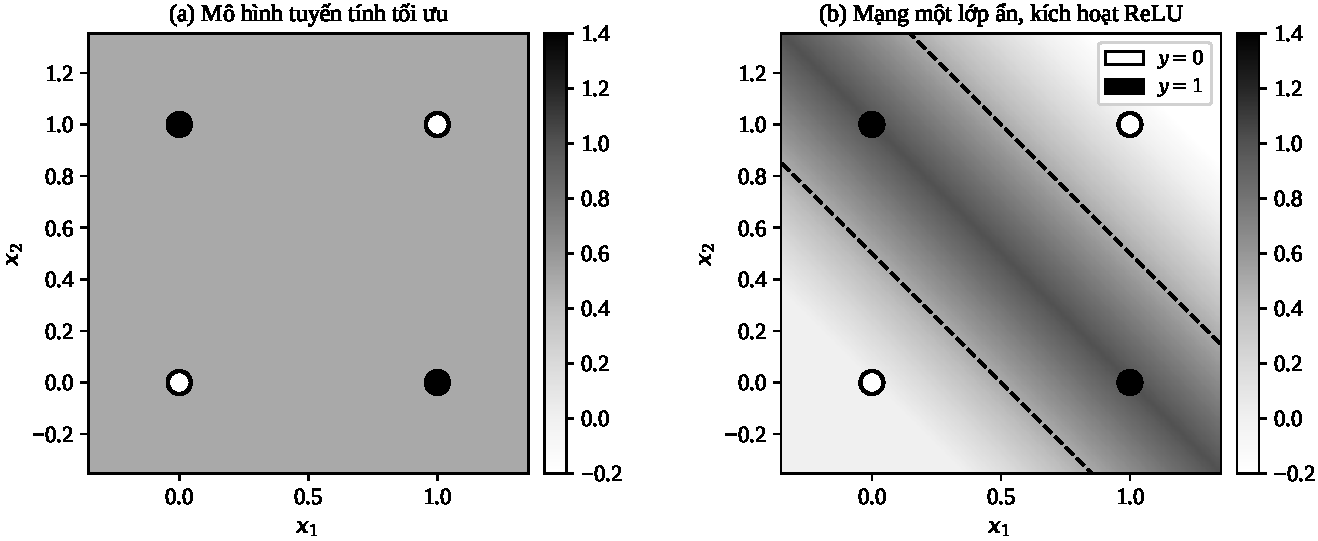
\includegraphics[width=0.95\textwidth]{Images/chap_2/hinh_xor.pdf}
\caption{Bài toán XOR. Điểm trắng ứng với $y=0$, điểm đen ứng với $y=1$; đường
đứt nét là mức $f = 0{,}5$. (a) Mô hình affine tối ưu là hằng số $0{,}5$ trên
toàn miền (Mệnh đề~\ref{md:xor-chan-duoi}), không có đường mức nào tách được dữ
liệu. (b) Mạng một lớp ẩn với tham số \eqref{eq:xor-net} tạo ra một dải giá trị
cao dọc theo đường $x_1+x_2=1$, tách đúng hai lớp.}
\label{fig:xor}
\end{figure}
 
\begin{nhanxet}
Hai điểm cần phân biệt rõ, cả hai đều sẽ tái xuất trong phần thực nghiệm.
 
Thứ nhất, Mệnh đề~\ref{md:xor-nghiem} chứng minh sự \emph{tồn tại} của bộ tham
số nghiệm, chứ không chứng minh rằng thuật toán tối ưu sẽ tìm được nó. Đây là
ranh giới giữa \emph{lý thuyết xấp xỉ} (khả năng biểu diễn) và \emph{lý thuyết
tối ưu} (khả năng học); ranh giới ấy được củng cố bởi
Mệnh đề~\ref{md:khong-loi} về tính không lồi.
 
Thứ hai, ví dụ này dùng ReLU và dùng tốt, trong khi Mục~\ref{sec:kichhoat} sẽ
loại trừ ReLU khỏi bài toán phương trình vi phân. Không có mâu thuẫn: ở đây ta
chỉ cần \emph{giá trị} của mạng khớp bốn nhãn, còn ở đó ta cần \emph{đạo hàm bậc
hai} của mạng khớp một phương trình. Tiêu chuẩn chọn hàm kích hoạt phụ thuộc vào
đại lượng nào của mạng được đưa vào hàm mục tiêu.
\end{nhanxet}
 
\subsection{Khả năng xấp xỉ phổ quát}
\label{subsec:xap-xi}
 
Ba định lý dưới đây trả lời ba câu hỏi khác nhau và thường bị gộp làm một trong
tài liệu phổ thông: mạng nơ-ron xấp xỉ được lớp hàm nào; xấp xỉ được theo
\emph{chuẩn} nào; và xấp xỉ với \emph{tốc độ} nào. Chỉ câu hỏi thứ hai và thứ ba
mới thực sự phục vụ báo cáo.
 
\begin{dinhly}[Xấp xỉ phổ quát, dạng $C^0$]
\label{dl:xap-xi}
Cho $K \subset \R^{d}$ compact và $\sigma \in C(\R)$ bị chặn địa phương. Tập các
hàm dạng
\begin{equation}
\Net(\bx) = \sum_{j=1}^{m} w_j\, \sigma\!\left( \bm{v}_j^{\top}\bx + c_j
\right),
\qquad m \in \mathbb{N}^{*},\ w_j, c_j \in \R,\ \bm{v}_j \in \R^{d},
\label{eq:xapxi}
\end{equation}
trù mật trong $C(K)$ với chuẩn hội tụ đều \emph{khi và chỉ khi} $\sigma$ không
phải là đa thức.
\end{dinhly}
 
\begin{nhanxet}[Về quy kết của Định lý~\ref{dl:xap-xi}]
\label{nx:quy-ket}
Dạng ``khi và chỉ khi $\sigma$ không phải đa thức'' ở trên là kết quả của Leshno
và cộng sự~\cite{leshno1993}, không phải của Cybenko hay Hornik. Cybenko
(\cite{cybenko1989}) chứng minh chiều thuận cho lớp hẹp hơn gồm các $\sigma$
\emph{sigmoidal}, tức liên tục với $\sigma(t)\to 1$ khi $t\to+\infty$ và
$\sigma(t)\to 0$ khi $t\to-\infty$. Việc phân biệt hai phát biểu là cần thiết
cho báo cáo: hàm $\sigma(t) = \sin t$ dùng trong một số kiến trúc PINN không
sigmoidal, nên chỉ nằm trong phạm vi của~\cite{leshno1993}. Chiều đảo của
Định lý~\ref{dl:xap-xi} chính là Mệnh đề~\ref{md:da-thuc} dưới đây, được chứng
minh đầy đủ vì lập luận sơ cấp và trực tiếp phục vụ tiêu chuẩn chọn $\sigma$.
\end{nhanxet}
 
\begin{proof}[Phác thảo chứng minh chiều thuận, theo Cybenko]
Ký hiệu $\mathcal{S}$ là bao đóng trong $C(K)$ của không gian sinh bởi các hàm
dạng \eqref{eq:xapxi}. Giả sử phản chứng $\mathcal{S} \ne C(K)$. Vì
$\mathcal{S}$ là không gian con đóng thực sự, theo định lý Hahn--Banach tồn tại
phiếm hàm tuyến tính liên tục $\Lambda \ne 0$ trên $C(K)$ triệt tiêu trên
$\mathcal{S}$. Theo định lý biểu diễn Riesz, tồn tại độ đo Borel chính quy hữu
hạn có dấu $\mu \ne 0$ sao cho $\Lambda(f) = \int_K f\,d\mu$. Khi đó
\[
\int_K \sigma(\bm{v}^{\top}\bx + c)\, d\mu(\bx) = 0
\qquad \forall\, \bm{v} \in \R^d,\ c \in \R .
\]
Bước then chốt là chứng minh rằng $\sigma$ trong lớp đang xét là \emph{phân
biệt} (discriminatory), tức đẳng thức trên buộc $\mu = 0$ -- mâu thuẫn. Ý tưởng:
dùng giả thiết về $\sigma$ để trích ra, qua phép lấy giới hạn khi tham số co
giãn tiến ra vô cùng, một hàm bậc thang; từ đó suy ra $\mu$ triệt tiêu trên mọi
nửa không gian, rồi kết luận bằng tính đầy đủ của hệ đặc trưng Fourier
$\bx\mapsto e^{i\bm{v}^{\top}\bx}$. Chi tiết đầy đủ xem~\cite{cybenko1989}; bản
sắc bén cho lớp không đa thức xem~\cite{leshno1993}.
\end{proof}
 
Đối với báo cáo này, dạng $C^0$ ở Định lý~\ref{dl:xap-xi} là \emph{chưa đủ}: nó
chỉ bảo đảm xấp xỉ giá trị hàm, không nói gì về đạo hàm. Một dãy hàm có thể hội
tụ đều tới $u$ trong khi đạo hàm của nó phân kỳ hoàn toàn; mà phần dư của phương
trình vi phân lại được xây trên đạo hàm. Dạng cần thiết là kết quả sau.
 
\begin{dinhly}[Hornik: xấp xỉ đồng thời đạo hàm]
\label{dl:sobolev}
Cho $K \subset \R^d$ compact, $k \in \mathbb{N}^{*}$, và $\sigma \in C^{k}(\R)$
không phải đa thức, với các đạo hàm tới bậc $k$ bị chặn. Khi đó tập các hàm dạng
\eqref{eq:xapxi} trù mật trong $C^{k}(K)$ theo chuẩn
\begin{equation}
\|f\|_{C^k(K)} = \max_{|\alpha| \le k}\ \sup_{\bx \in K}
  \big| \partial^{\alpha} f(\bx) \big| ,
\label{eq:chuan-ck}
\end{equation}
tức với mọi $f \in C^k(K)$ và $\varepsilon > 0$ tồn tại $\Net$ dạng
\eqref{eq:xapxi} sao cho $\|f - \Net\|_{C^k(K)} < \varepsilon$. Nói riêng, tập
ấy cũng trù mật trong không gian Sobolev $W^{k,\infty}(K)$.
\end{dinhly}
 
Định lý~\ref{dl:sobolev} (\cite{hornik1991}) là mệnh đề bảo đảm nền tảng cho
toàn bộ phương pháp: nếu nghiệm đúng $u$ của một phương trình vi phân bậc $k$
thuộc $C^k(K)$, thì tồn tại mạng nơ-ron làm nhỏ tuỳ ý cả sai số nghiệm lẫn sai
số của mọi đạo hàm tới bậc $k$, do đó làm nhỏ tuỳ ý phần dư. Hai điều kiện của
định lý đều mang tính bắt buộc và đều dẫn thẳng sang Mục~\ref{sec:kichhoat}:
$\sigma$ phải \emph{thuộc lớp $C^k$} và phải \emph{không là đa thức}.
 
Cần nhấn mạnh giới hạn của kết quả này. Nó khẳng định sự \emph{tồn tại} của một
bộ tham số tốt; nó không cho biết cần bao nhiêu nơ-ron, cũng không cho biết
thuật toán tối ưu có tìm được bộ tham số ấy hay không. Câu hỏi thứ nhất được
định lượng một phần bởi định lý sau; câu hỏi thứ hai vẫn để ngỏ trong toàn bộ
lĩnh vực.
 
\begin{dinhly}[Barron: tốc độ xấp xỉ]
\label{dl:barron}
Giả sử $f : \R^d \to \R$ có biến đổi Fourier $\hat f$ thoả mãn
\begin{equation}
C_f := \int_{\R^d} \|\bm{\omega}\|\,\big|\hat f(\bm{\omega})\big|\,
  d\bm{\omega} < \infty .
\label{eq:barron-hang-so}
\end{equation}
Khi đó với mọi $m \in \mathbb{N}^{*}$, tồn tại mạng một lớp ẩn $\Net_m$ với $m$
nơ-ron sigmoidal sao cho
\begin{equation}
\int_{K} \big( f(\bx) - \Net_m(\bx) \big)^2 \mu(d\bx)
 \;\le\; \frac{(2 r C_f)^2}{m},
\label{eq:barron}
\end{equation}
với $K$ là quả cầu bán kính $r$ và $\mu$ là độ đo xác suất tuỳ ý trên $K$.
\end{dinhly}
 
\begin{nhanxet}[Vì sao mạng nơ-ron hấp dẫn với bài toán nhiều chiều]
\label{nx:loi-nguyen}
Chặn \eqref{eq:barron} (\cite{barron1993}) có bậc $\mathcal{O}(m^{-1/2})$
\emph{không phụ thuộc số chiều $d$}; số chiều chỉ ẩn trong hằng số $C_f$. Trái
lại, các phương pháp xấp xỉ tuyến tính cổ điển -- đa thức, phần tử hữu hạn, lưới
sai phân -- trên lớp hàm trơn bậc $s$ chỉ đạt bậc $\mathcal{O}(m^{-s/d})$, suy
giảm nhanh khi $d$ tăng; đó là ``lời nguyền số chiều''. Đây là lập luận định
lượng chính biện minh cho việc dùng mạng nơ-ron thay cho lưới trong các bài toán
phương trình vi phân nhiều chiều.
 
Hai điều kiện phải đọc kèm. Thứ nhất, sự chuyển dịch phụ thuộc chiều từ
\emph{bậc} sang \emph{hằng số} không phải là sự biến mất của nó: với nhiều lớp
hàm, $C_f$ tự nó tăng theo $d$. Thứ hai, \eqref{eq:barron} là chặn theo chuẩn
$L^2$ chứ không phải chuẩn $C^k$ của Định lý~\ref{dl:sobolev}; không có kết quả
nào trong báo cáo cho phép ghép trực tiếp tốc độ của Barron với chuẩn cần thiết
cho phần dư. Ta dẫn Định lý~\ref{dl:barron} như một lập luận \emph{định hướng},
không như một chặn sai số áp dụng được cho các thí nghiệm ở
Chương~\ref{chap:thucnghiem}.
\end{nhanxet}
 
%==============================================================================
\section{Hàm kích hoạt}
\label{sec:kichhoat}
%==============================================================================
 
\subsection{Bốn điều kiện và nguồn gốc của chúng}
\label{subsec:yeu-cau}
 
Trong tài liệu học sâu, việc chọn hàm kích hoạt thường được trình bày như một
vấn đề kinh nghiệm --- xem chẳng hạn Mục 6.2.2 của Goodfellow và cộng
sự~\cite{goodfellow2016} hay phần khảo sát hàm kích hoạt
của Hammad~\cite{hammad2024}, nơi các hàm được so sánh chủ yếu theo hiệu quả
huấn luyện. Trong bài toán phương trình vi phân, phần lớn lựa chọn bị
ràng buộc bởi các kết quả đã thiết lập ở Mục~\ref{sec:cautruc}. Tổng hợp Hệ
quả~\ref{hq:suy-bien}, Hệ quả~\ref{hq:relu-hessian} và Định lý~\ref{dl:sobolev},
hàm kích hoạt $\sigma$ cần thoả mãn:
 
\begin{enumerate}[label=(\roman*), leftmargin=*]
\item \textbf{Không affine} -- điều kiện cần để mạng không suy biến thành ánh xạ
      affine (Hệ quả~\ref{hq:suy-bien}).
\item \textbf{Không đa thức} -- điều kiện cần và đủ cho tính trù mật
      (Định lý~\ref{dl:xap-xi}; chiều cần được chứng minh ở
      Mệnh đề~\ref{md:da-thuc}).
\item \textbf{Thuộc lớp $C^{k}$ với $k$ bằng bậc cao nhất của toán tử vi phân},
      và $\sigma^{(k)} \not\equiv 0$ (Hệ quả~\ref{hq:relu-hessian} và
      Nhận xét~\ref{nx:bac-cao}).
\item \textbf{Hành vi gradient lành mạnh} -- tích các $\sigma'$ dọc theo chiều
      sâu không được suy giảm hay bùng nổ quá nhanh
      (Mệnh đề~\ref{md:tich-gradient}).
\end{enumerate}
 
Ba điều kiện đầu là điều kiện \emph{cần} theo nghĩa toán học chặt chẽ: vi phạm
một trong ba thì phương pháp hỏng, không phải hoạt động kém. Điều kiện (iv) có
tính chất khác, là một yêu cầu định lượng về thang số và có thể được bù đắp một
phần bằng khởi tạo (Mục~\ref{sec:khoitao}).
 
\begin{menhde}[Hàm kích hoạt đa thức là không đủ]
\label{md:da-thuc}
Nếu $\sigma$ là đa thức bậc $p \ge 1$ thì mọi mạng theo
Định nghĩa~\ref{def:fnn} với $L$ lớp biểu diễn một đa thức bậc không quá
$p^{\,L-1}$. Do đó tập các hàm biểu diễn được nằm trong một không gian vectơ
hữu hạn chiều, là tập đóng và thực sự con của $C(K)$; nói riêng nó \emph{không}
trù mật trong $C(K)$.
\end{menhde}
 
\begin{proof}
Ta chứng minh bằng quy nạp rằng mỗi thành phần của $\ba^{(\ell)}$ là đa thức
theo $\bx$ với bậc không quá $p^{\ell}$.
 
Cơ sở $\ell = 0$: $\ba^{(0)} = \bx$ có bậc $1 = p^{0}$.
 
Bước quy nạp: theo \eqref{eq:z-k}, $z^{(\ell)}_k$ là tổ hợp tuyến tính của các
thành phần $a^{(\ell-1)}_j$ cộng hằng số, nên có bậc không quá $p^{\ell-1}$; hợp
thành với đa thức $\sigma$ bậc $p$ cho $a^{(\ell)}_k = \sigma(z^{(\ell)}_k)$ bậc
không quá $p\cdot p^{\ell-1} = p^{\ell}$.
 
Lớp ra là tổ hợp tuyến tính của $\ba^{(L-1)}$ nên $\Net_{\btheta}$ có bậc không
quá $p^{\,L-1}$.
 
Không gian các đa thức $d$ biến bậc không quá $D := p^{L-1}$ có số chiều
$\binom{D+d}{d} < \infty$. Mọi không gian con hữu hạn chiều của một không gian
định chuẩn đều đóng, và nó thực sự con vì $C(K)$ chứa các hàm không đa thức
(chẳng hạn $e^{x_1}$, với $K$ có phần trong khác rỗng). Vậy bao đóng của nó
không thể bằng $C(K)$.
\end{proof}
 
Điểm đáng chú ý: chặn $p^{L-1}$ tăng rất nhanh theo $L$, nên một mạng đa thức
sâu vẫn biểu diễn được các đa thức bậc rất cao. Sự thất bại ở đây không phải là
thất bại về \emph{dung lượng} mà về \emph{loại}: dù $L$ lớn đến đâu, lớp hàm thu
được vẫn nằm trong một không gian hữu hạn chiều đóng, và một hàm đơn giản như
$e^{x_1}$ mãi mãi nằm ngoài tầm với ở khoảng cách dương.
 
\subsection{Các hàm kích hoạt thông dụng}
 
\begin{table}[H]
\centering
\caption{So sánh các hàm kích hoạt thông dụng; $\sigma_{\mathrm{s}}$ ký hiệu
hàm sigmoid logistic. Cột cuối đối chiếu với điều kiện (iii) của
Mục~\ref{subsec:yeu-cau} cho toán tử bậc hai.}
\label{tab:kichhoat}
\small
\begin{tabular}{@{}l c c c c c@{}}
\toprule
\textbf{Tên} & \textbf{Biểu thức} & \textbf{Đạo hàm bậc nhất}
  & \textbf{Miền giá trị} & \textbf{Độ trơn} & $\sigma''\!\not\equiv\!0$ \\
\midrule
Sigmoid & $\dfrac{1}{1+e^{-z}}$
  & $\sigma_{\mathrm{s}}(1-\sigma_{\mathrm{s}})$ & $(0,1)$ & $C^{\infty}$
  & có \\[6pt]
Tanh & $\dfrac{e^{z}-e^{-z}}{e^{z}+e^{-z}}$
  & $1-\tanh^{2}z$ & $(-1,1)$ & $C^{\infty}$ & có \\[6pt]
ReLU & $\max\{0,z\}$
  & $\mathbf{1}_{\{z>0\}}$ & $[0,+\infty)$ & $C^{0}$ & \textbf{không} \\[6pt]
Leaky ReLU & $\max\{\alpha z, z\}$
  & $\mathbf{1}_{\{z>0\}} + \alpha\mathbf{1}_{\{z<0\}}$ & $\R$ & $C^{0}$
  & \textbf{không} \\[6pt]
Softplus & $\ln(1+e^{z})$
  & $\sigma_{\mathrm{s}}(z)$ & $(0,+\infty)$ & $C^{\infty}$ & có \\[6pt]
Swish (SiLU) & $z\,\sigma_{\mathrm{s}}(z)$
  & $\sigma_{\mathrm{s}} + z\sigma_{\mathrm{s}}(1-\sigma_{\mathrm{s}})$
  & $\approx[-0{,}28,+\infty)$ & $C^{\infty}$ & có \\[6pt]
Sine & $\sin z$ & $\cos z$ & $[-1,1]$ & $C^{\infty}$ & có \\
\bottomrule
\end{tabular}
\end{table}
 
\begin{figure}[H]
\centering
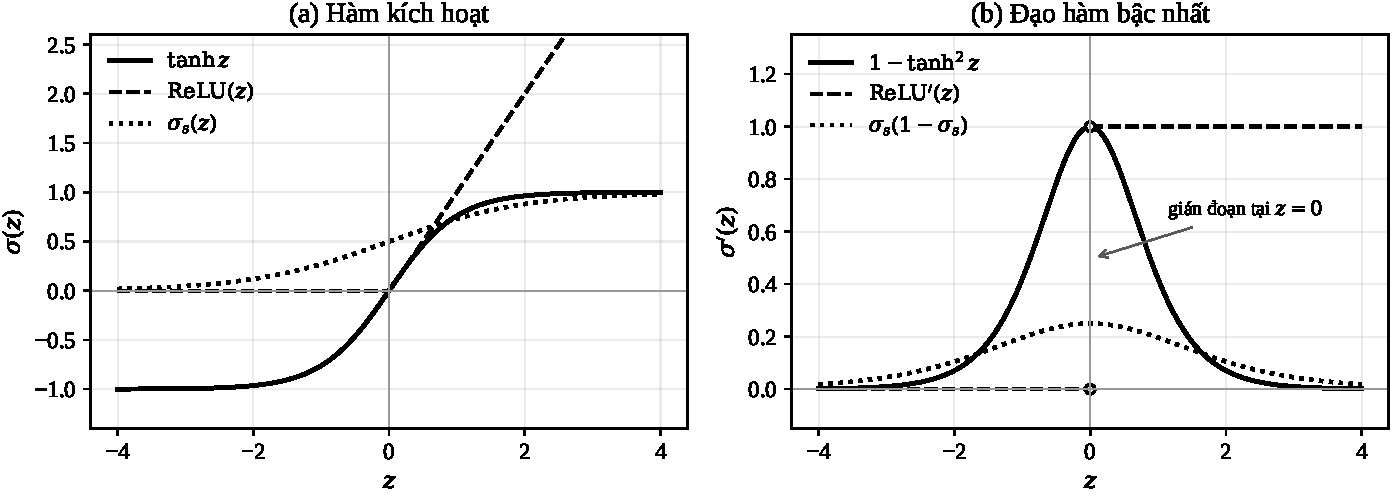
\includegraphics[width=0.98\textwidth]{Images/chap_2/hinh_kichhoat.pdf}
\caption{(a) Đồ thị ba hàm kích hoạt tiêu biểu. (b) Đạo hàm bậc nhất tương ứng.
Điểm gãy của ReLU tại $z=0$ thể hiện thành bước nhảy đơn vị của
$\mathrm{ReLU}'$. Đồng thời có thể thấy $\tanh'$ và $\sigma_{\mathrm{s}}'$ đều
tắt nhanh khi $|z| \gtrsim 3$, minh hoạ hiện tượng bão hoà được lượng hoá ở
Mệnh đề~\ref{md:tich-gradient}.}
\label{fig:kichhoat}
\end{figure}
 
\subsection{Giải tích của hàm tanh}
\label{subsec:tanh}
 
Vì $\tanh$ là hàm kích hoạt được chọn cho toàn bộ phần thực nghiệm, mục này
thiết lập ba tính chất của nó mà các chương sau sẽ dùng: cấu trúc đại số của đạo
hàm bậc cao, chặn đều cho mọi đạo hàm, và tốc độ tăng của đạo hàm tại gốc.
 
\begin{bode}[Cấu trúc đa thức của đạo hàm bậc cao]
\label{bd:tanh-dao-ham}
Đặt $\sigma(z) = \tanh z$. Tồn tại dãy đa thức $\{P_k\}_{k\ge 0}$ một biến sao
cho
\begin{equation}
\sigma^{(k)}(z) = P_k\big(\sigma(z)\big), \qquad k \ge 0,
\label{eq:tanh-Pk}
\end{equation}
xác định bởi $P_0(t) = t$ và hệ thức truy hồi
\begin{equation}
P_{k+1}(t) = \big(1 - t^2\big)\, P_k'(t).
\label{eq:tanh-truy-hoi}
\end{equation}
Hơn nữa $\deg P_k = k+1$ với mọi $k \ge 0$.
\end{bode}
 
\begin{proof}
Với $k = 0$, \eqref{eq:tanh-Pk} là định nghĩa của $P_0$. Giả sử
$\sigma^{(k)} = P_k \circ \sigma$. Lấy đạo hàm và dùng
$\sigma' = 1 - \sigma^2$ (suy trực tiếp từ
$\tanh' = \sech^2 = 1 - \tanh^2$):
\[
\sigma^{(k+1)}(z) = P_k'\big(\sigma(z)\big)\,\sigma'(z)
 = P_k'\big(\sigma(z)\big)\big(1 - \sigma(z)^2\big)
 = P_{k+1}\big(\sigma(z)\big),
\]
với $P_{k+1}$ cho bởi \eqref{eq:tanh-truy-hoi}.
 
Về bậc: $\deg P_0 = 1$ với hệ số dẫn đầu $c_0 = 1$. Nếu $\deg P_k = k+1$ với hệ
số dẫn đầu $c_k \ne 0$ thì $\deg P_k' = k$ với hệ số dẫn đầu $(k+1)c_k$, và nhân
với $(1-t^2)$ cho $\deg P_{k+1} = k+2$ với hệ số dẫn đầu $-(k+1)c_k \ne 0$. Quy
nạp kết thúc.
\end{proof}
 
Ba phần tử đầu của dãy, thu được bằng cách áp dụng
\eqref{eq:tanh-truy-hoi} hai lần:
\begin{align}
\sigma'(z)   &= 1 - \sigma^{2}, \label{eq:tanh-d1}\\
\sigma''(z)  &= -2\sigma\left(1-\sigma^{2}\right)
             = -2\sigma + 2\sigma^3, \label{eq:tanh-d2}\\
\sigma'''(z) &= -2\left(1-\sigma^{2}\right)\left(1-3\sigma^{2}\right)
             = -2 + 8\sigma^2 - 6\sigma^4. \label{eq:tanh-d3}
\end{align}
Công thức \eqref{eq:tanh-d2} là công thức được dùng ở Ví dụ~\ref{vd:dao-ham} và
ở dòng 6 của Thuật toán~\ref{alg:dao-ham}. Điểm thực hành đáng lưu ý: nhờ
\eqref{eq:tanh-Pk}, mọi đạo hàm bậc cao của $\tanh$ được tính \emph{chỉ từ giá
trị $\tanh z$ đã có}, không cần đánh giá lại hàm mũ.
 
\begin{hequa}[Chặn đều cho mọi đạo hàm]
\label{hq:tanh-chan}
Với mọi $k \ge 0$,
\begin{equation}
\sup_{z\in\R} \big|\sigma^{(k)}(z)\big|
 \;\le\; \max_{|t| \le 1} \big|P_k(t)\big| =: M_k < \infty .
\label{eq:tanh-chan}
\end{equation}
Cụ thể $M_0 = 1$, $M_1 = 1$, $M_2 = \dfrac{4}{3\sqrt{3}} \approx 0{,}7698$.
\end{hequa}
 
\begin{proof}
Vì $\sigma(\R) = (-1,1) \subset [-1,1]$, kết hợp \eqref{eq:tanh-Pk} với tính
liên tục của $P_k$ trên compact $[-1,1]$ cho \eqref{eq:tanh-chan}. Giá trị
$M_0 = \max_{|t|\le1}|t| = 1$. Giá trị $M_1 = \max_{|t|\le1}|1-t^2| = 1$, đạt
tại $t = 0$. Giá trị $M_2$: xét $h(t) = -2t + 2t^3$ trên $[-1,1]$; ta có
$h'(t) = -2 + 6t^2 = 0$ tại $t = \pm 1/\sqrt3$, cho
$|h| = 2/\sqrt3 - 2/(3\sqrt3) = 4/(3\sqrt3)$, còn tại hai đầu mút $h(\pm1) = 0$.
\end{proof}
 
Hệ quả~\ref{hq:tanh-chan} có ý nghĩa thực hành trực tiếp: nó cho phép chặn đều
mọi số hạng chứa $\sigma^{(m)}$ trong hệ truy hồi \eqref{eq:S-truy-hoi}, bảo đảm
rằng đạo hàm bậc cao của mạng $\tanh$ \emph{không thể} bùng nổ do bản thân hàm
kích hoạt. Nếu $\nabla^2_{\bx}\Net_{\btheta}$ bùng nổ trong thực nghiệm, nguyên
nhân chỉ có thể là trọng số lớn -- tức là vấn đề khởi tạo hoặc vấn đề tối ưu,
không phải vấn đề kiến trúc. Đây là một tiêu chuẩn chẩn đoán hữu ích khi gỡ lỗi
huấn luyện.
 
\begin{menhde}[Tính giải tích và bán kính hội tụ]
\label{md:tanh-giai-tich}
Hàm $\tanh$ chỉnh hình trên dải
$\{z \in \mathbb{C} : |\operatorname{Im} z| < \pi/2\}$ và có cực điểm đơn tại
$z = \pm i\pi/2$. Do đó chuỗi Taylor của $\tanh$ tại $0$ có bán kính hội tụ đúng
bằng $\pi/2$, và
\begin{equation}
\limsup_{k\to\infty}
  \left(\frac{\big|\sigma^{(k)}(0)\big|}{k!}\right)^{\!1/k}
 = \frac{2}{\pi},
\qquad\text{tức}\qquad
\forall\,\epsilon>0\ \ \exists\, C_\epsilon:\;
\big|\sigma^{(k)}(0)\big| \le C_\epsilon\, k!
  \left(\frac{2}{\pi}+\epsilon\right)^{\!k} .
\label{eq:tanh-tang}
\end{equation}
\end{menhde}
 
\begin{proof}
$\tanh z = \sinh z/\cosh z$ là thương của hai hàm nguyên; các điểm kỳ dị là
nghiệm của $\cosh z = 0$, tức $z = i\pi/2 + ik\pi$, $k \in \mathbb{Z}$. Điểm kỳ
dị gần gốc nhất cách gốc $\pi/2$, nên bán kính hội tụ bằng $\pi/2$. Đẳng thức
\eqref{eq:tanh-tang} chính là công thức Cauchy--Hadamard áp cho hệ số Taylor
$a_k = \sigma^{(k)}(0)/k!$: bán kính hội tụ $R = \big(\limsup_k
|a_k|^{1/k}\big)^{-1}$ bằng $\pi/2$. Dạng thứ hai suy ra từ định nghĩa của
$\limsup$.
\end{proof}
 
\begin{nhanxet}[Vì sao không viết được chặn với đúng cơ số $2/\pi$]
Bất đẳng thức Cauchy cho $|a_k| \le M(r)/r^{k}$ với mọi $r < \pi/2$, trong đó
$M(r) = \max_{|z|=r}|\tanh z|$; nhưng $M(r) \to \infty$ khi $r \to \pi/2^{-}$ vì
$\tanh$ có cực tại $i\pi/2$, nên \emph{không} thể chọn $r = \pi/2$ để thu được
chặn dạng $|\sigma^{(k)}(0)| \le C\,k!\,(2/\pi)^k$ chỉ bằng lập luận này. Chặn
với đúng cơ số $2/\pi$ vẫn đúng, nhưng đòi hỏi khai triển thặng dư tại cực đơn
$i\pi/2$ chứ không phải bất đẳng thức Cauchy. Vì báo cáo chỉ cần \emph{bậc}
tăng, ta dừng ở \eqref{eq:tanh-tang}.
\end{nhanxet}
 
Mệnh đề~\ref{md:tanh-giai-tich} lý giải một quan sát thực nghiệm quen thuộc: vi
phân tự động bậc cao trên mạng $\tanh$ ổn định về số, vì các đạo hàm tại gốc chỉ
tăng theo cấp giai thừa với cơ số $2/\pi < 1$, chứ không nhanh hơn. Trong thực hành, các phương
trình được xét ở báo cáo này có bậc không quá $2$, nên chỉ cần
\eqref{eq:tanh-d1}--\eqref{eq:tanh-d2}.
 
\subsection{Cấu trúc của mạng ReLU}
\label{subsec:relu}
 
Mục này giải thích, bằng hai lối lập luận độc lập, vì sao ReLU -- lựa chọn mặc
định gần như tuyệt đối trong thị giác máy tính -- lại vắng bóng hoàn toàn trong
tài liệu về phương trình vi phân.
 
\begin{dinhly}[Mạng ReLU là hàm tuyến tính từng khúc]
\label{dl:relu-tuyen-tinh}
Với $\sigma = \mathrm{ReLU}$, tồn tại một họ hữu hạn các đa diện lồi
$\{\Omega_1,\dots,\Omega_R\}$ có phần trong rời nhau, phủ $\R^{n_0}$, sao cho
$\Net_{\btheta}$ trùng với một ánh xạ affine trên mỗi $\Omega_r$.
\end{dinhly}
 
\begin{proof}
Ta chứng minh bằng quy nạp theo $\ell$ rằng tồn tại phân hoạch đa diện hữu hạn
$\mathcal{P}^{(\ell)}$ của $\R^{n_0}$ sao cho $\ba^{(\ell)}$ là affine trên mỗi
ô.
 
Cơ sở $\ell = 0$: $\ba^{(0)} = \bx$ affine trên
$\mathcal{P}^{(0)} = \{\R^{n_0}\}$.
 
Bước quy nạp: trên mỗi ô $\Omega \in \mathcal{P}^{(\ell-1)}$, $\ba^{(\ell-1)}$
affine, nên $\bz^{(\ell)} = \bW^{(\ell)}\ba^{(\ell-1)} + \bb^{(\ell)}$ cũng
affine trên $\Omega$; viết $z^{(\ell)}_k(\bx) = \bm{\alpha}_k^{\top}\bx +
\beta_k$ trên $\Omega$. Chia $\Omega$ bởi $n_\ell$ siêu phẳng
$H_k = \{\bm{\alpha}_k^{\top}\bx + \beta_k = 0\}$ thành tối đa $2^{n_\ell}$ ô
con, mỗi ô con vẫn là đa diện lồi (giao của $\Omega$ với các nửa không gian).
Trên mỗi ô con, dấu của $z^{(\ell)}_k$ không đổi với mọi $k$, nên
$a^{(\ell)}_k = \max\{0, z^{(\ell)}_k\}$ bằng $z^{(\ell)}_k$ hoặc bằng $0$ --
trong cả hai trường hợp đều affine. Lấy $\mathcal{P}^{(\ell)}$ là họ tất cả các
ô con thu được; đó là họ hữu hạn vì $\mathcal{P}^{(\ell-1)}$ hữu hạn.
 
Cuối cùng, lớp ra là ánh xạ affine của $\ba^{(L-1)}$ nên $\Net_{\btheta}$ affine
trên mỗi ô của $\mathcal{P}^{(L-1)}$.
\end{proof}
 
\begin{hequa}[Hessian triệt tiêu hầu khắp nơi]
\label{hq:relu-hkn}
Với $\sigma = \mathrm{ReLU}$,
\begin{equation}
\nabla^2_{\bx} \Net_{\btheta}(\bx) = \bm{0}
\qquad \text{với hầu khắp } \bx \in \R^{n_0}
\ (\text{theo độ đo Lebesgue}).
\label{eq:relu-hessian-zero}
\end{equation}
\end{hequa}
 
\begin{proof}
Theo Định lý~\ref{dl:relu-tuyen-tinh}, $\Net_{\btheta}$ affine trên phần trong
của mỗi $\Omega_r$, nên Hessian triệt tiêu ở đó. Phần bù
$\R^{n_0}\setminus\bigcup_r \operatorname{int}\Omega_r$ chứa trong hợp hữu hạn
các siêu phẳng, là tập có độ đo Lebesgue bằng $0$.
\end{proof}
 
Kết luận \eqref{eq:relu-hessian-zero} cũng suy được từ Hệ
quả~\ref{hq:relu-hessian} bằng cách áp dụng nó tại mỗi $\bx$ nằm ngoài tập điểm
gãy, nơi $\sigma'' = 0$ trên một lân cận. Hai lối chứng minh soi sáng hai mặt
khác nhau của cùng một hiện tượng: một mặt hình học (phân hoạch đa diện), một
mặt giải tích (truy hồi độ cong). Mệnh đề sau cho biết ``phần độ cong bị mất''
đã đi đâu.
 
\begin{menhde}[Đạo hàm bậc hai theo nghĩa phân bố, trường hợp một chiều]
\label{md:dirac}
Xét $n_0 = n_L = 1$, $L = 2$, tức
$\Net(x) = \sum_{j=1}^{m} w_j\,\mathrm{ReLU}(v_j x + c_j) + b$ với
$v_j \ne 0$. Khi đó, theo nghĩa phân bố trên $\mathcal{D}'(\R)$,
\begin{equation}
\Net'' = \sum_{j=1}^{m} w_j\, |v_j|\; \delta_{x_j},
\qquad x_j := -\,c_j/v_j .
\label{eq:dirac}
\end{equation}
Nói riêng, $\Net''$ là một tổ hợp tuyến tính hữu hạn các độ đo Dirac, có giá là
tập hữu hạn $\{x_1,\dots,x_m\}$ có độ đo Lebesgue bằng $0$.
\end{menhde}
 
\begin{proof}
Đủ xét một số hạng $u(x) = \mathrm{ReLU}(vx+c)$. Vì $u$ liên tục và tuyến tính
từng khúc, đạo hàm phân bố của nó là
$u'(x) = v\,\mathbf{1}_{\{vx+c>0\}}$. Hàm chỉ báo này là hàm bậc thang với bước
nhảy tại $x_0 = -c/v$: nếu $v > 0$ thì $\{vx+c>0\} = (x_0,\infty)$ và chỉ báo
nhảy từ $0$ lên $1$; nếu $v<0$ thì $\{vx+c>0\} = (-\infty,x_0)$ và chỉ báo nhảy
từ $1$ xuống $0$. Trong cả hai trường hợp biên độ bước nhảy là
$\operatorname{sgn}(v)$. Đạo hàm phân bố của hàm bậc thang Heaviside là $\delta$,
nên
\[
u'' = v \cdot \operatorname{sgn}(v)\,\delta_{x_0} = |v|\,\delta_{x_0}.
\]
Lấy tổ hợp tuyến tính với hệ số $w_j$ và dùng tính tuyến tính của đạo hàm phân
bố cho \eqref{eq:dirac}.
\end{proof}
 
Cần đọc \eqref{eq:dirac} cho đúng: đạo hàm bậc hai của mạng ReLU không phải là
$0$; nó là một phân bố kỳ dị. Nhưng vi phân tự động không tính phân bố, nó tính
giá trị điểm; và tại hầu khắp mọi điểm, giá trị ấy bằng $0$. Chính khoảng cách
giữa hai khái niệm đạo hàm này sinh ra hệ quả sau.
 
\subsection{Hệ quả đối với bài toán phương trình vi phân}
 
\begin{hequa}[Sụp đổ của gradient huấn luyện với kiến trúc ReLU]
\label{hq:pinn-hong}
Xét bài toán $-u''(x) = f(x)$ trên $\Omega \subset \R$ và hàm mục tiêu phần dư
\begin{equation}
J(\btheta) = \frac{1}{N_r}\sum_{i=1}^{N_r}
  \Big( -\Net''_{\btheta}(x_i) - f(x_i) \Big)^{2}.
\label{eq:J-residual}
\end{equation}
Giả sử $\sigma = \mathrm{ReLU}$ và các điểm phối trí $x_i$ được lấy mẫu từ một
phân phối liên tục tuyệt đối trên $\Omega$. Khi đó, với xác suất $1$, tồn tại
lân cận $U$ của $\btheta$ trong $\R^P$ sao cho
\begin{equation}
J(\btheta') = \frac{1}{N_r}\sum_{i=1}^{N_r} f(x_i)^2
\quad \forall\, \btheta' \in U,
\qquad\text{và do đó}\qquad
\nabla_{\btheta} J(\btheta) = \bm{0}.
\label{eq:gradient-zero}
\end{equation}
\end{hequa}
 
\begin{proof}
Theo Định lý~\ref{dl:relu-tuyen-tinh}, phân hoạch $\mathcal{P}^{(L-1)}$ của
$\R$ là hữu hạn, nên tập điểm gãy $\mathcal{K}(\btheta)$ -- hợp các biên của các
ô -- là tập hữu hạn, do đó có độ đo Lebesgue $0$. Vì phân phối lấy mẫu liên tục
tuyệt đối, $\mathbb{P}\big(\exists\, i:\ x_i \in \mathcal{K}(\btheta)\big) = 0$.
Vậy với xác suất $1$, mọi $x_i$ đều nằm trong phần trong của một ô, nơi
$\Net''_{\btheta}(x_i) = 0$ theo Hệ quả~\ref{hq:relu-hkn}.
 
Hơn nữa, điều vừa nói tương đương với $z^{(\ell)}_k(x_i) \ne 0$ với mọi
$i,\ell,k$, vì các điểm gãy đúng là nơi một tiền kích hoạt đổi dấu. Mỗi hàm
$\btheta' \mapsto z^{(\ell)}_k(x_i)$ liên tục (hợp thành của các phép affine và
ReLU, đều liên tục), và bộ ba chỉ số $(i,\ell,k)$ chạy trên một tập
\emph{hữu hạn}. Vậy tồn tại lân cận $U$ của $\btheta$ mà trên đó cả hữu hạn
đại lượng ấy đều giữ nguyên dấu, nói riêng không triệt tiêu: không một điểm gãy
nào có thể rơi trúng một $x_i$ khi $\btheta'$ còn nằm trong $U$. Trên $U$ ta có
$\Net''_{\btheta'}(x_i) = 0$ với mọi $i$; thay vào \eqref{eq:J-residual} cho
$J$ hằng trên $U$ với giá trị nêu ở \eqref{eq:gradient-zero}. Một hàm hằng địa
phương có gradient bằng $0$.
\end{proof}
 
Hệ quả~\ref{hq:pinn-hong} phát biểu chính xác điều mà tài liệu thường chỉ mô tả
định tính. Điểm cần nhấn mạnh: đây \emph{không} phải hiện tượng ``hội tụ chậm''
hay ``khó tối ưu''. Hàm mục tiêu là \emph{hằng số địa phương}, nên mọi thuật
toán dựa trên gradient -- SGD, Adam, L-BFGS~\cite{nocedal2006} -- đều đứng yên
tuyệt đối tại mọi điểm khởi tạo. Mô hình nằm ngoài không gian hàm chứa nghiệm,
và không có cách tinh chỉnh siêu tham số nào cứu vãn được.
 
\begin{nhanxet}
Lập luận trên cũng giải thích vì sao các hàm kích hoạt trơn khác -- softplus,
Swish, sine -- vẫn được xem xét trong tài liệu về phương trình vi
phân~\cite{karniadakis2021}, trong khi ReLU thì không. Với phương trình bậc nhất
($\mathcal{L} = \partial_x$), ReLU về nguyên tắc dùng được vì $\Net'$ không đồng
nhất triệt tiêu; nhưng khi ấy $\Net'$ là hàm bậc thang, không thể xấp xỉ tốt một
đạo hàm liên tục theo chuẩn đều -- đúng như Định lý~\ref{dl:sobolev} dự báo, vì
ReLU không thuộc $C^1$.
\end{nhanxet}
 
\subsection{Bão hoà và triệt tiêu gradient}
\label{subsec:bao-hoa}
 
Ưu thế về độ trơn của $\tanh$ không miễn phí. Kết quả sau lượng hoá cái giá phải
trả, và là nội dung của điều kiện (iv) ở Mục~\ref{subsec:yeu-cau}.
 
\begin{menhde}[Chặn tích gradient theo chiều sâu]
\label{md:tich-gradient}
Đặt $\bm{\delta}^{(\ell)} = \partial J/\partial\bz^{(\ell)}$. Từ quy tắc dây
chuyền, $\bm{\delta}^{(\ell-1)} = \bD^{(\ell-1)}
\big(\bW^{(\ell)}\big)^{\!\top}\bm{\delta}^{(\ell)}$, và do đó
\begin{equation}
\big\|\bm{\delta}^{(1)}\big\|_2
 \;\le\; \big\|\bm{\delta}^{(L)}\big\|_2
   \prod_{\ell=2}^{L} \big\|\bW^{(\ell)}\big\|_2
   \prod_{\ell=1}^{L-1} \big\|\bD^{(\ell)}\big\|_2 .
\label{eq:chan-gradient}
\end{equation}
Với $\sigma = \tanh$ ta có
$\|\bD^{(\ell)}\|_2 = \max_k \big(1 - \tanh^2 z^{(\ell)}_k\big) \le 1$; nếu
ngoài ra $|z^{(\ell)}_k| \ge \tau$ với mọi $k,\ell$ thì
\begin{equation}
\big\|\bm{\delta}^{(1)}\big\|_2 \;\le\;
\big\|\bm{\delta}^{(L)}\big\|_2 \left(\prod_{\ell=2}^{L}
\big\|\bW^{(\ell)}\big\|_2\right)
\sech^{2(L-1)}(\tau),
\label{eq:chan-bao-hoa}
\end{equation}
tức thừa số do bão hoà đóng góp vào chặn trên suy giảm theo cấp số nhân với cơ
số $\sech^{2}(\tau) < 1$. Cần đọc \eqref{eq:chan-bao-hoa} cho đúng: đây là chặn
\emph{trên}, và nó chỉ kéo theo gradient thực sự triệt tiêu khi tích
$\prod_{\ell=2}^{L}\|\bW^{(\ell)}\|_2$ không bù lại được sự suy giảm ấy -- điều
được bảo đảm dưới khởi tạo Xavier (Mục~\ref{sec:khoitao}), nơi mỗi
$\|\bW^{(\ell)}\|_2$ ở thang $\mathcal{O}(1)$.
\end{menhde}
 
\begin{proof}
Hệ thức truy hồi cho $\bm{\delta}$ là quy tắc dây chuyền chuẩn, được dẫn chi
tiết ở Chương~\ref{chap:autodiff}. Bất đẳng thức \eqref{eq:chan-gradient} suy từ
tính nhân dưới của chuẩn phổ, $\|\bm{A}\bu\|_2 \le \|\bm{A}\|_2\|\bu\|_2$, áp
dụng lặp. Với $\bD$ đường chéo, $\|\bD\|_2$ bằng giá trị tuyệt đối lớn nhất trên
đường chéo, ở đây là $\max_k \sech^2 z^{(\ell)}_k$. Cuối cùng,
$1 - \tanh^2 t = \sech^2 t$ là hàm chẵn, giảm ngặt trên $[0,\infty)$, nên
$|z| \ge \tau$ kéo theo $\sech^2 z \le \sech^2 \tau$.
\end{proof}
 
Ví dụ số cho thấy mức độ nghiêm trọng (lấy
$\prod_{\ell}\|\bW^{(\ell)}\|_2 = 1$ để cô lập riêng ảnh hưởng của bão hoà): với
$\tau = 3$ ta có
$\sech^2(3) \approx 0{,}00987$; qua $L-1 = 10$ lớp bão hoà, hệ số suy giảm là
$0{,}00987^{10} \approx 8{,}7\times10^{-21}$ -- gradient bị triệt tiêu hoàn toàn
trong số học dấu phẩy động độ chính xác kép, nơi epsilon máy vào cỡ
$2{,}2\times10^{-16}$. Đây chính là lý do Mục~\ref{sec:khoitao} là bắt buộc chứ
không phải tuỳ chọn: phải giữ $|z^{(\ell)}|$ nhỏ ngay từ thời điểm khởi tạo, vì
một khi mạng đã bão hoà thì không còn tín hiệu gradient để thoát ra.
 
\subsection{Kiểm chứng số}
 
Thí nghiệm TN-B kiểm chứng \eqref{eq:tanh-d1}--\eqref{eq:tanh-d3} bằng sai phân
hữu hạn trung tâm tại năm điểm rải trên $[-2;\,3]$. Sai số tối đa thu được lần
lượt là $3{,}3\times10^{-9}$, $9{,}0\times10^{-9}$ và $4{,}4\times10^{-5}$ cho
đạo hàm bậc một, hai và ba -- hoàn toàn tương thích với bậc chính xác của các
lược đồ sai phân được dùng, trong đó lược đồ bậc ba nhạy cảm nhất với sai số làm
tròn do chia cho $h^3$.
 
Cùng thí nghiệm định lượng Hệ quả~\ref{hq:relu-hkn} trên lưới $501$ điểm với
mạng ReLU $H = 32$ nơ-ron: $97{,}8\%$ số điểm cho $|\Net''_{\btheta}| < 1$ với
giá trị cực đại chỉ $5{,}0\times10^{-10}$, đúng bằng mức sai số làm tròn của
lược đồ sai phân; $11$ điểm còn lại nằm sát các điểm gãy và cho giá trị bùng nổ.
Đây là biểu hiện số của các độ đo Dirac trong \eqref{eq:dirac}: sai phân hữu hạn
với bước $h$ ``nhìn thấy'' một Dirac dưới dạng một xung biên độ
$\mathcal{O}(1/h)$ khi điểm lưới rơi gần điểm gãy.
 
%==============================================================================
\section{Khởi tạo trọng số và độ chệch}
\label{sec:khoitao}
%==============================================================================
 
Mục~\ref{sec:kichhoat} kết luận rằng phải giữ $|z^{(\ell)}|$ nhỏ tại thời điểm
bắt đầu huấn luyện. Mục này biến yêu cầu định tính ấy thành một công thức cho
phương sai của trọng số khởi tạo, qua ba bước: loại trừ khởi tạo hằng
(Mục~\ref{subsec:doi-xung}), thiết lập điều kiện bảo toàn phương sai
(Mục~\ref{subsec:phuong-sai}), và hiệu chỉnh sai lệch bậc hai giữa lý thuyết và
thực nghiệm (Mục~\ref{subsec:hieu-chinh}).
 
\subsection{Phá vỡ đối xứng}
\label{subsec:doi-xung}
 
\begin{menhde}[Khởi tạo hằng làm suy biến bề rộng]
\label{md:doi-xung}
Giả sử tại thời điểm khởi tạo, với mỗi $\ell$ tồn tại các hằng số
$c_\ell, d_\ell \in \R$ sao cho
\begin{equation}
w^{(\ell)}_{kj} = c_\ell \ \ \forall k,j,
\qquad
b^{(\ell)}_k = d_\ell \ \ \forall k .
\label{eq:khoi-tao-hang}
\end{equation}
Khi huấn luyện bằng gradient descent toàn phần, tính chất
\eqref{eq:khoi-tao-hang} được bảo toàn qua mọi bước lặp. Nói riêng, mọi nơ-ron
trong cùng một lớp luôn có cùng kích hoạt và cùng gradient, nên lớp $\ell$ hành
xử như lớp chỉ có một nơ-ron, bất kể $n_\ell$ lớn đến đâu. Trường hợp riêng
$c_\ell = d_\ell = 0$ là khởi tạo bằng không.
\end{menhde}
 
\begin{proof}
Quy nạp theo số bước lặp. Giả sử \eqref{eq:khoi-tao-hang} đúng với mọi $\ell$
tại bước hiện tại; ta chứng minh nó vẫn đúng sau một bước cập nhật.
 
\emph{Bước 1: kích hoạt hằng theo thành phần.} Từ \eqref{eq:z-k},
$z^{(1)}_k = c_1\sum_j x_j + d_1$ không phụ thuộc $k$, nên các thành phần của
$\ba^{(1)}$ bằng nhau. Quy nạp theo $\ell$: nếu các thành phần của
$\ba^{(\ell-1)}$ bằng nhau, ký hiệu chung là $\bar a^{(\ell-1)}$, thì
$z^{(\ell)}_k = c_\ell\, n_{\ell-1}\, \bar a^{(\ell-1)} + d_\ell$ không phụ
thuộc $k$. Vậy mọi $\ba^{(\ell)}$ đều có các thành phần bằng nhau, và ta ký hiệu
$\bar z^{(\ell)}, \bar a^{(\ell)}$ cho giá trị chung.
 
\emph{Bước 2: sai số ngược hằng theo thành phần.} Ta chứng minh quy nạp lùi rằng
các thành phần của $\bm{\delta}^{(\ell)}$ bằng nhau. Tại lớp ra, điều này hiển
nhiên khi $n_L = 1$; với $n_L > 1$ nó đúng khi hàm mất mát đối xứng theo các
thành phần đầu ra, điều thoả mãn với MSE. Giả sử các thành phần của
$\bm{\delta}^{(\ell+1)}$ bằng nhau và bằng $\bar\delta^{(\ell+1)}$. Từ
$\bm{\delta}^{(\ell)} = \bD^{(\ell)}\big(\bW^{(\ell+1)}\big)^{\!\top}
\bm{\delta}^{(\ell+1)}$, thành phần thứ $k$ là
\[
\delta^{(\ell)}_k
 = \sigma'\!\big(\bar z^{(\ell)}\big)
   \sum_{i=1}^{n_{\ell+1}} w^{(\ell+1)}_{ik}\,\delta^{(\ell+1)}_i
 = \sigma'\!\big(\bar z^{(\ell)}\big)\, c_{\ell+1}\, n_{\ell+1}\,
   \bar\delta^{(\ell+1)},
\]
không phụ thuộc $k$. Ở đây ta đã dùng \emph{đầy đủ} giả thiết
\eqref{eq:khoi-tao-hang}: $w^{(\ell+1)}_{ik} = c_{\ell+1}$ với mọi cặp chỉ số.
 
\emph{Bước 3: gradient là ma trận hằng.} Ta có
$\partial J/\partial w^{(\ell)}_{kj} = \delta^{(\ell)}_k\, a^{(\ell-1)}_j
 = \bar\delta^{(\ell)}\,\bar a^{(\ell-1)}$, không phụ thuộc cả $k$ lẫn $j$;
tương tự $\partial J/\partial b^{(\ell)}_k = \bar\delta^{(\ell)}$ không phụ
thuộc $k$. Vậy bước cập nhật
$\bW^{(\ell)} \gets \bW^{(\ell)} - \eta\,\partial J/\partial\bW^{(\ell)}$ trừ đi
cùng một số khỏi mọi phần tử, nên \eqref{eq:khoi-tao-hang} được bảo toàn với các
hằng số mới. Lập luận tương tự cho $\bb^{(\ell)}$.
\end{proof}
 
\begin{nhanxet}[Về một giả thiết yếu hơn và không đủ]
\label{nx:phan-vi-du}
Trong tài liệu, mệnh đề trên đôi khi được phát biểu với giả thiết yếu hơn: ``mọi
\emph{hàng} của $\bW^{(\ell)}$ bằng nhau''. Giả thiết ấy đủ cho Bước 1 nhưng
\emph{không} được bảo toàn qua bước cập nhật, nên phát biểu đó không đúng. Thật
vậy, nếu $\bW^{(\ell+1)}$ chỉ có các hàng bằng nhau, tức
$w^{(\ell+1)}_{ik} = \omega_k$ phụ thuộc $k$, thì Bước 2 cho
\[
\delta^{(\ell)}_k
 = \sigma'\!\big(\bar z^{(\ell)}\big)\,\omega_k
   \sum_{i} \delta^{(\ell+1)}_i
 = C\,\omega_k ,
\]
phụ thuộc $k$. Khi đó hàng thứ $k$ của ma trận gradient bằng
$C\,\omega_k\,\big(\ba^{(\ell-1)}\big)^{\!\top}$: các hàng chỉ \emph{tỉ lệ} với
nhau chứ không bằng nhau, và sau một bước cập nhật tính chất ``các hàng bằng
nhau'' bị phá vỡ. Nói cách khác, đối xứng thực sự được bảo toàn là đối xứng
\emph{hoán vị đầy đủ} giữa các nơ-ron trong một lớp, mà \eqref{eq:khoi-tao-hang}
là điều kiện đủ tự nhiên nhất để có nó.
\end{nhanxet}
 
Mệnh đề~\ref{md:doi-xung} loại trừ khởi tạo hằng: trọng số phải được khởi tạo
\emph{ngẫu nhiên}. Câu hỏi còn lại là với phương sai bằng bao nhiêu.
 
\subsection{Phân tích lan truyền phương sai}
\label{subsec:phuong-sai}
 
\begin{bode}[Phương sai của tổ hợp tuyến tính ngẫu nhiên]
\label{bd:phuong-sai}
Cho $W_1,\dots,W_n$ độc lập cùng phân phối với $\E W_j = 0$, $\Var W_j = v$, và
$a_1,\dots,a_n$ độc lập với $\{W_j\}$ và có $\E[a_j^2] < \infty$. Đặt
$z = \sum_{j=1}^{n} W_j a_j$. Khi đó
\begin{equation}
\E[z] = 0, \qquad
\Var(z) = \E[z^2] = v \sum_{j=1}^{n} \E\big[a_j^2\big]
        = n\, v\, \E\big[a^2\big]
\label{eq:bo-de-var}
\end{equation}
(đẳng thức cuối khi các $a_j$ cùng phân phối).
\end{bode}
 
\begin{proof}
Do độc lập, $\E[z] = \sum_j \E[W_j]\,\E[a_j] = 0$. Tiếp theo
\[
\E[z^2] = \sum_{j}\sum_{k} \E\big[W_j W_k a_j a_k\big]
        = \sum_{j}\sum_{k} \E\big[W_j W_k\big]\, \E\big[a_j a_k\big],
\]
trong đó bước thứ hai dùng tính độc lập giữa họ $\{W\}$ và họ $\{a\}$. Vì các
$W_j$ độc lập với kỳ vọng $0$, $\E[W_jW_k] = v\,\delta_{jk}$. Vậy tổng kép thu
về đường chéo và cho \eqref{eq:bo-de-var}.
\end{proof}
 
Một điểm tinh tế đáng nêu ngay, vì nó là mấu chốt phân biệt hai công thức khởi
tạo ở hai mục sau: đại lượng xuất hiện ở vế phải \eqref{eq:bo-de-var} là
\emph{mômen bậc hai} $\E[a^2]$, không phải phương sai $\Var(a)$. Hai đại lượng
chỉ trùng nhau khi $\E[a] = 0$ -- điều đúng với $\tanh$ (hàm lẻ, nên kích hoạt
đối xứng quanh $0$ khi $z$ đối xứng) nhưng \emph{sai} với ReLU và sigmoid, vốn
cho kích hoạt không âm.
 
Ta làm việc với các giả thiết sau, theo tinh thần Mục 8.4 của Goodfellow và cộng
sự~\cite{goodfellow2016}:
 
\begin{enumerate}[label=(A\arabic*), leftmargin=*]
\item Các phần tử $w^{(\ell)}_{kj}$ độc lập cùng phân phối, kỳ vọng $0$, phương
      sai $v_\ell := \Var\!\big(w^{(\ell)}\big)$.
\item $\bb^{(\ell)} = \bm{0}$.
\item Các kích hoạt $a^{(\ell-1)}_j$ độc lập với trọng số của lớp $\ell$ và độc
      lập cùng phân phối với nhau.
\item (Tuyến tính hoá) $\sigma(t) \approx \sigma'(0)\,t$ trên miền giá trị thực
      tế của $z$. Với $\tanh$, $\sigma'(0) = 1$ nên $\sigma(t)\approx t$.
\end{enumerate}
 
Cần nói thẳng rằng (A3) là một giả thiết \emph{sai} về mặt chặt chẽ: sau lớp thứ
nhất, các kích hoạt trong cùng một lớp phụ thuộc lẫn nhau vì chúng dùng chung
đầu vào. Giả thiết này được chấp nhận vì nó cho một dự đoán bậc nhất đúng và
kiểm chứng được; Mục~\ref{subsec:hieu-chinh} sẽ chỉ ra đúng chỗ mà phân tích này
lệch khỏi thực nghiệm, và bù lại phần lệch bằng một hiệu chỉnh từ (A4) chứ không
từ (A3).
 
\begin{menhde}[Truy hồi phương sai xuôi]
\label{md:var-xuoi}
Dưới (A1)--(A3),
\begin{equation}
\E\Big[\big(z^{(\ell)}\big)^2\Big]
 = n_{\ell-1}\, v_\ell\; \E\Big[\big(a^{(\ell-1)}\big)^2\Big].
\label{eq:lan-truyen-phuong-sai}
\end{equation}
Nếu thêm (A4) thì $\E[(a^{(\ell)})^2] \approx \E[(z^{(\ell)})^2]$, và do đó
\begin{equation}
\E\Big[\big(z^{(L)}\big)^2\Big]
 \;\approx\; \E\big[x^2\big] \prod_{\ell=1}^{L} n_{\ell-1}\, v_\ell .
\label{eq:tich-luy}
\end{equation}
\end{menhde}
 
\begin{proof}
Hệ thức \eqref{eq:lan-truyen-phuong-sai} là Bổ đề~\ref{bd:phuong-sai} áp dụng
cho hàng thứ $k$ của $\bW^{(\ell)}$ với $n = n_{\ell-1}$, dùng \eqref{eq:z-k} và
(A2). Áp dụng lặp qua các lớp và dùng (A4) ở mỗi lớp cho \eqref{eq:tich-luy}.
\end{proof}
 
\begin{hequa}[Tăng hoặc giảm theo cấp số nhân]
\label{hq:cap-so-nhan}
Đặt $\rho_\ell := n_{\ell-1} v_\ell$. Nếu $\rho_\ell \equiv \rho$ với mọi $\ell$
thì $\E[(z^{(L)})^2] \approx \rho^{L}\,\E[x^2]$. Do đó $\rho < 1$ kéo theo suy
giảm mũ về $0$, $\rho > 1$ kéo theo bùng nổ mũ, và chỉ $\rho = 1$ bảo toàn thang
tín hiệu.
\end{hequa}
 
Điều kiện $\rho = 1$ cho \emph{chiều xuôi} là
\begin{equation}
v_\ell = \frac{1}{n_{\ell-1}} .
\label{eq:dk-xuoi}
\end{equation}
 
Bảo toàn tín hiệu xuôi là chưa đủ: huấn luyện dùng gradient, và gradient lan
truyền theo chiều ngược với một hệ thức truy hồi khác.
 
\begin{menhde}[Truy hồi phương sai ngược]
\label{md:var-nguoc}
Với $\bm{\delta}^{(\ell)} = \partial J/\partial\bz^{(\ell)}$ và các giả thiết
tương ứng (A1)--(A4) áp cho chiều ngược,
\begin{equation}
\E\Big[\big(\delta^{(\ell-1)}\big)^2\Big]
 = n_{\ell}\, v_\ell\; \E\Big[\big(\delta^{(\ell)}\big)^2\Big]
   \cdot \big(\sigma'(0)\big)^2 ,
\label{eq:var-nguoc}
\end{equation}
nên điều kiện bảo toàn chiều ngược (với $\sigma'(0)=1$) là
\begin{equation}
v_\ell = \frac{1}{n_{\ell}} .
\label{eq:dk-nguoc}
\end{equation}
\end{menhde}
 
\begin{proof}
Từ $\bm{\delta}^{(\ell-1)} = \bD^{(\ell-1)}\big(\bW^{(\ell)}\big)^{\!\top}
\bm{\delta}^{(\ell)}$, thành phần thứ $j$ là
\[
\delta^{(\ell-1)}_j = \sigma'\!\big(z^{(\ell-1)}_j\big)
\sum_{i=1}^{n_\ell} w^{(\ell)}_{ij}\,\delta^{(\ell)}_i .
\]
Tổng có $n_\ell$ số hạng -- lưu ý sự khác biệt với \eqref{eq:z-k}, nơi tổng có
$n_{\ell-1}$ số hạng; đây chính là nguồn gốc của mâu thuẫn giữa
\eqref{eq:dk-xuoi} và \eqref{eq:dk-nguoc}. Áp dụng Bổ đề~\ref{bd:phuong-sai} với
$n = n_\ell$, rồi nhân thêm $\big(\sigma'(0)\big)^2$ theo (A4).
\end{proof}
 
\subsection{Khởi tạo Xavier (Glorot)}
\label{subsec:xavier}
 
Hai điều kiện \eqref{eq:dk-xuoi} và \eqref{eq:dk-nguoc} chỉ tương thích khi
$n_{\ell-1} = n_{\ell}$, tức khi mạng có bề rộng đều. Với kiến trúc tổng quát,
không tồn tại $v_\ell$ thoả cả hai. Glorot và Bengio~\cite{glorot2010} đề xuất
dung hoà bằng cách lấy \emph{trung bình điều hoà của hai phương sai ứng viên}
$1/n_{\ell-1}$ và $1/n_{\ell}$ -- tương đương nghịch đảo trung bình cộng của
$n_{\ell-1}$ và $n_{\ell}$:
\begin{equation}
\boxed{\;
v_\ell = \Var\!\left(w^{(\ell)}\right) = \frac{2}{n_{\ell-1} + n_{\ell}} \; }
\label{eq:xavier}
\end{equation}
Cần nhận rõ bản chất của \eqref{eq:xavier}: đó là một \emph{thoả hiệp} giữa hai
điều kiện không đồng thời thoả mãn được, không phải nghiệm của một bài toán tối
ưu nào. Khi $n_{\ell-1} = n_\ell = n$, thoả hiệp trở thành chính xác:
$v_\ell = 1/n$ và cả hai điều kiện cùng được thoả.
 
\begin{menhde}[Dạng phân phối đều của Xavier]
\label{md:xavier-deu}
Nếu $w^{(\ell)}_{kj} \sim \mathcal{U}(-\alpha,\alpha)$ thì
$v_\ell = \alpha^2/3$. Do đó \eqref{eq:xavier} tương đương với
\begin{equation}
w^{(\ell)}_{kj} \sim
\mathcal{U}\!\left( -\sqrt{\frac{6}{n_{\ell-1}+n_{\ell}}},\;
                     \sqrt{\frac{6}{n_{\ell-1}+n_{\ell}}} \right).
\label{eq:xavier-uniform}
\end{equation}
\end{menhde}
 
\begin{proof}
Với $U \sim \mathcal{U}(-\alpha,\alpha)$ ta có $\E U = 0$ và
$\Var U = \E U^2 = \frac{1}{2\alpha}\int_{-\alpha}^{\alpha} t^2\,dt
= \frac{\alpha^2}{3}$. Đặt $\alpha^2/3 = 2/(n_{\ell-1}+n_\ell)$ và giải theo
$\alpha > 0$ cho $\alpha = \sqrt{6/(n_{\ell-1}+n_\ell)}$.
\end{proof}

\begin{nhanxet}[Dạng đều và dạng chuẩn tắc là tương đương với mọi kết quả của
chương]
\label{nx:xavier-dang}
Toàn bộ phân tích ở Mục~\ref{subsec:phuong-sai} chỉ dùng ba tính chất của phân
phối khởi tạo: kỳ vọng $0$, các phần tử độc lập cùng phân phối, và phương sai
bằng $v_\ell$. Không kết quả nào phụ thuộc \emph{dạng} của phân phối. Do đó
\eqref{eq:xavier-uniform} và dạng chuẩn tắc
$w^{(\ell)}_{kj}\sim\mathcal{N}\big(0,\,2/(n_{\ell-1}+n_\ell)\big)$ đều hiện thực
hoá đúng điều kiện \eqref{eq:xavier} và đều dùng được. Ta ghi rõ điều này vì
phần thực nghiệm ở Chương~\ref{chap:thucnghiem} dùng dạng chuẩn tắc
(\texttt{xavier\_normal\_}), còn chương này nêu dạng đều làm ví dụ cụ thể.
\end{nhanxet}
 
\subsection{Khởi tạo He}
\label{subsec:he}
 
\begin{bode}[Mất một nửa mômen bậc hai qua ReLU]
\label{bd:relu-nua}
Nếu $z$ là biến ngẫu nhiên đối xứng quanh $0$ (tức $z$ và $-z$ cùng phân phối)
với $\E[z^2] < \infty$, thì
\begin{equation}
\E\Big[\big(\max\{0,z\}\big)^2\Big] = \tfrac{1}{2}\,\E\big[z^2\big].
\label{eq:relu-nua-phuong-sai}
\end{equation}
\end{bode}
 
\begin{proof}
Ta có $\big(\max\{0,z\}\big)^2 = z^2\,\mathbf{1}_{\{z>0\}}$. Do tính đối xứng,
$z^2\mathbf{1}_{\{z>0\}}$ và $z^2\mathbf{1}_{\{z<0\}}$ cùng phân phối, nên có
cùng kỳ vọng. Mặt khác
$z^2\mathbf{1}_{\{z>0\}} + z^2\mathbf{1}_{\{z<0\}} = z^2$ hầu chắc chắn (tập
$\{z=0\}$ đóng góp $0$ vào cả hai vế). Lấy kỳ vọng hai vế và chia đôi.
\end{proof}
 
Bổ đề~\ref{bd:relu-nua} nói rằng giả thiết (A4) sai đúng một hệ số $\tfrac12$
đối với ReLU: mỗi lớp làm mất một nửa mômen bậc hai. Bù lại hệ số ấy trong
\eqref{eq:dk-xuoi}, He và cộng sự~\cite{he2015} đề xuất
\begin{equation}
\boxed{\;
v_\ell = \Var\!\left(w^{(\ell)}\right) = \frac{2}{n_{\ell-1}} \; }
\label{eq:he}
\end{equation}
 
\begin{table}[H]
\centering
\caption{Đối chiếu ba chiến lược khởi tạo. LeCun là trường hợp riêng ứng với
việc chỉ áp điều kiện xuôi \eqref{eq:dk-xuoi}.}
\label{tab:khoitao}
\small
\begin{tabular}{@{}l c c c@{}}
\toprule
& \textbf{LeCun} & \textbf{Xavier (Glorot)} & \textbf{He} \\
\midrule
Giả thiết về $\sigma$ & đối xứng & đối xứng, $\sigma'(0)\approx1$
  & ReLU / Leaky ReLU \\
$\Var(w)$ & $1/n_{\text{in}}$ & $2/(n_{\text{in}}+n_{\text{out}})$
  & $2/n_{\text{in}}$ \\
Biên phân phối đều & $\sqrt{3/n_{\text{in}}}$
  & $\sqrt{6/(n_{\text{in}}+n_{\text{out}})}$ & $\sqrt{6/n_{\text{in}}}$ \\
Điều kiện được thoả & xuôi & dung hoà xuôi/ngược & xuôi, có bù $\tfrac12$ \\
Dùng trong báo cáo & không & \textbf{có} (với $\tanh$) & không \\
\bottomrule
\end{tabular}
\end{table}
 
Bảng~\ref{tab:khoitao} cho thấy lý do báo cáo chọn Xavier chứ không phải He
không nằm ở chất lượng của công thức mà ở \emph{phạm vi áp dụng}: He được suy ra
riêng cho ReLU thông qua Bổ đề~\ref{bd:relu-nua}, mà ReLU đã bị loại trừ ở
Hệ quả~\ref{hq:pinn-hong}. Dùng \eqref{eq:he} với $\tanh$ sẽ cho $\rho = 2$, tức
bùng nổ theo Hệ quả~\ref{hq:cap-so-nhan}.
 
\subsection{Hiệu chỉnh bậc hai và quy luật suy giảm điều hoà}
\label{subsec:hieu-chinh}
 
Giả thiết tuyến tính hoá (A4) dự đoán rằng với $\rho = 1$, phương sai được bảo
toàn \emph{chính xác} qua mọi lớp. Thực nghiệm (Bảng~\ref{tab:so-lieu-khoitao})
lại cho thấy phương sai suy giảm đều đặn. Đây là một sai lệch có hệ thống giữa
lý thuyết và số liệu, và nó cần được giải thích chứ không bỏ qua. Mệnh đề sau
định lượng sai lệch đó bằng cách giữ lại số hạng bậc hai mà (A4) đã bỏ.
 
\begin{menhde}[Suy giảm điều hoà của phương sai với $\tanh$]
\label{md:hieu-chinh}
Xét mạng bề rộng đều $n_\ell \equiv n$ với khởi tạo Xavier, khi đó
$\rho = n\,v = 1$. Đặt $s_\ell^2 := \E\big[(a^{(\ell)})^2\big]$ và giả sử
$z^{(\ell)} \sim \mathcal{N}(0, s_{\ell-1}^2)$. Khi đó
\begin{equation}
s_\ell^2 = s_{\ell-1}^2 - 2\,s_{\ell-1}^4 + \mathcal{O}\big(s_{\ell-1}^6\big),
\label{eq:hieu-chinh}
\end{equation}
và do đó, khi $\ell \to \infty$,
\begin{equation}
s_\ell^2 \;\sim\; \frac{1}{2\ell}.
\label{eq:dieu-hoa}
\end{equation}
\end{menhde}
 
\begin{proof}
Khai triển Taylor $\tanh t = t - \tfrac{t^3}{3} + \tfrac{2t^5}{15} -\cdots$ cho
$\tanh^2 t = t^2 - \tfrac{2}{3}t^4 + \mathcal{O}(t^6)$ khi $t \to 0$. Chuỗi này
chỉ hội tụ với $|t| < \pi/2$ (Mệnh đề~\ref{md:tanh-giai-tich}), trong khi biến
Gauss $z$ nhận giá trị trên toàn $\R$; vì vậy \emph{không} được phép lấy kỳ vọng
từng số hạng của chuỗi. Ta thay bằng một chặn phần dư đúng trên toàn trục. Đặt
\[
\psi(t) := \tanh^2 t - \Big(t^2 - \tfrac{2}{3}t^4\Big).
\]
Hàm $\psi$ liên tục, $\psi(t) = \mathcal{O}(t^6)$ khi $t\to 0$, và vì
$\tanh^2$ bị chặn bởi $1$ nên $|\psi(t)| \le 1 + t^2 + \tfrac23 t^4$ với mọi $t$.
Hai tính chất ấy cho một hằng số $C$ (không phụ thuộc $t$) sao cho
\begin{equation}
\big|\psi(t)\big| \;\le\; C\,t^{6}
\qquad\text{với mọi } t \in \R,
\label{eq:chan-phan-du-tanh}
\end{equation}
bởi trên $[-1,1]$ hàm $t \mapsto \psi(t)/t^6$ liên tục (kỳ dị tại $0$ khử được)
nên bị chặn, còn với $|t| \ge 1$ ta có $1 \le t^4$ và $t^2 \le t^4$, do đó
$|\psi(t)| \le \tfrac83 t^4 \le \tfrac83 t^6$.

Với $z \sim \mathcal{N}(0,s^2)$ ta có $\E[z^2] = s^2$, $\E[z^4] = 3s^4$ và
$\E[z^6] = 15 s^6$. Lấy kỳ vọng hai vế của
$\tanh^2 z = z^2 - \tfrac23 z^4 + \psi(z)$ rồi dùng
\eqref{eq:chan-phan-du-tanh}:
\[
\Big| \E\big[\tanh^2 z\big] - \big(s^2 - 2s^4\big) \Big|
 \;=\; \big|\E[\psi(z)]\big| \;\le\; C\,\E\big[z^6\big] \;=\; 15\,C\,s^{6},
\]
tức $s_\ell^2 = \E[\tanh^2 z^{(\ell)}] = s^2 - 2s^4 + \mathcal{O}(s^6)$ với
$s = s_{\ell-1}$, do $\rho = 1$ kéo theo $\Var(z^{(\ell)}) = s_{\ell-1}^2$
theo \eqref{eq:lan-truyen-phuong-sai}. Đó là \eqref{eq:hieu-chinh}, và số hạng
dư nay là một chặn \emph{đều} chứ không phải một khai triển hình thức.
 
Để suy ra \eqref{eq:dieu-hoa}, đặt $u_\ell := 1/s_\ell^2$. Từ
\eqref{eq:hieu-chinh},
\[
u_\ell = \frac{1}{s_{\ell-1}^2\big(1 - 2s_{\ell-1}^2 + \mathcal{O}(s^4)\big)}
       = u_{\ell-1}\Big(1 + 2s_{\ell-1}^2 + \mathcal{O}(s^4)\Big)
       = u_{\ell-1} + 2 + \mathcal{O}\big(s_{\ell-1}^2\big).
\]
Vì \eqref{eq:hieu-chinh} cho $s_\ell^2 < s_{\ell-1}^2$ khi $s_{\ell-1}$ đủ nhỏ,
dãy $(s_\ell^2)$ giảm ngặt và bị chặn dưới bởi $0$ nên hội tụ; giới hạn $s^2$
phải thoả $s^2 = s^2 - 2s^4$, tức $s = 0$. Do đó số hạng dư
$\mathcal{O}(s_{\ell-1}^2) \to 0$, và theo định lý trung bình Cesàro,
$u_\ell/\ell \to 2$, tức $u_\ell \sim 2\ell$ và $s_\ell^2 \sim 1/(2\ell)$.
\end{proof}
 
\begin{nhanxet}[Ý nghĩa thực hành]
\label{nx:y-nghia-dieu-hoa}
Kết luận \eqref{eq:dieu-hoa} quan trọng hơn vẻ ngoài kỹ thuật của nó. Nó cho
biết sự suy giảm phương sai dưới khởi tạo Xavier là \emph{đa thức} (bậc
$\ell^{-1}$), \emph{không phải cấp số nhân}. Đối chiếu với
Hệ quả~\ref{hq:cap-so-nhan}: một sai lệch dù nhỏ khỏi $\rho = 1$ gây suy giảm mũ
$\rho^\ell$, còn khi $\rho = 1$ chính xác thì phần phi tuyến của $\tanh$ chỉ gây
suy giảm điều hoà. Đó là lý do Xavier vẫn dùng tốt cho mạng vài chục lớp: sau
$30$ lớp, $s^2 \approx 1/60$, vẫn cách rất xa ngưỡng tràn số dưới. Nói cách
khác, giá trị của điều kiện $\rho = 1$ không phải là bảo toàn phương sai một
cách chính xác -- điều đó không xảy ra -- mà là \emph{đổi cơ chế suy giảm từ mũ
sang đa thức}.
\end{nhanxet}
 
\subsection{Kiểm chứng số}
 
\begin{figure}[H]
\centering
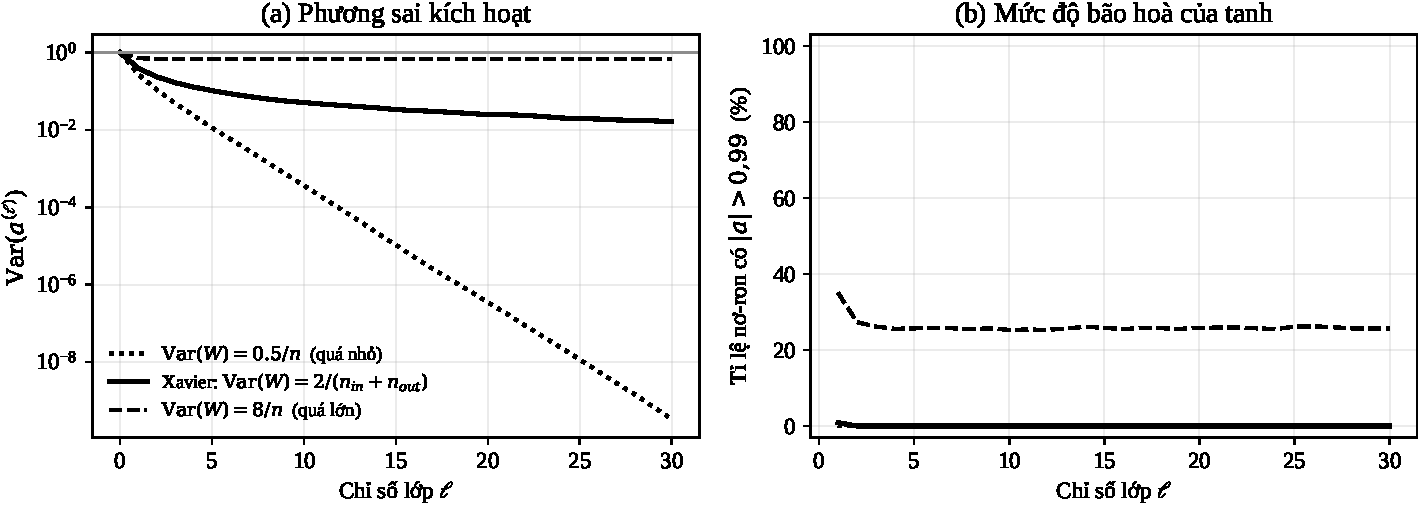
\includegraphics[width=0.98\textwidth]{Images/chap_2/hinh_khoitao.pdf}
\caption{Lan truyền tín hiệu xuôi qua $30$ lớp, mỗi lớp $256$ nơ-ron, kích hoạt
$\tanh$. (a) Phương sai kích hoạt theo thang log. Khi $\rho = 0{,}5 < 1$, phương
sai suy giảm theo cấp số nhân đúng như Hệ quả~\ref{hq:cap-so-nhan}; đường Xavier
($\rho = 1$) suy giảm chậm hơn hẳn, phù hợp quy luật điều hoà
\eqref{eq:dieu-hoa}. (b) Tỉ lệ nơ-ron bão hoà. Cấu hình $\rho = 8$ giữ được
phương sai chỉ nhờ $\tanh$ chặn giá trị, nhưng phải trả giá bằng khoảng $26\%$
nơ-ron rơi vào vùng $\sigma' \approx 0$.}
\label{fig:khoitao}
\end{figure}
 
\begin{figure}[H]
\centering
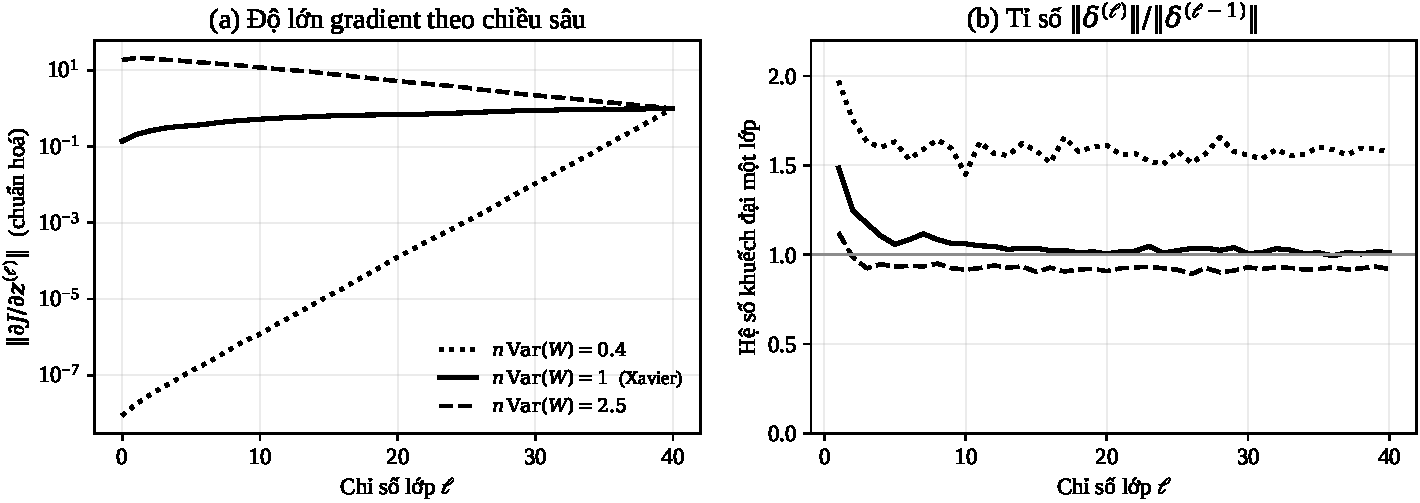
\includegraphics[width=0.98\textwidth]{Images/chap_2/hinh_gradient.pdf}
\caption{Lan truyền gradient ngược qua $40$ lớp, minh hoạ
Mệnh đề~\ref{md:tich-gradient}. (a) Chuẩn $\|\bm{\delta}^{(\ell)}\|$ theo thang
log: với $\rho = 0{,}4$, gradient tại lớp đầu nhỏ hơn tại lớp cuối khoảng $8$
bậc thập phân -- triệt tiêu gradient hoàn toàn. (b) Hệ số khuếch đại một lớp
$\|\bm{\delta}^{(\ell)}\|/\|\bm{\delta}^{(\ell-1)}\|$; đường Xavier bám sát mức
$1$, đúng như thiết kế của điều kiện \eqref{eq:dk-nguoc}.}
\label{fig:gradient}
\end{figure}
 
\begin{table}[H]
\centering
\caption{Kết quả thí nghiệm TN-C: mạng $12$ lớp, mỗi lớp $128$ nơ-ron, kích hoạt
$\tanh$, lô $N = 400$ mẫu chuẩn tắc. Cột ``bão hoà'' là tỉ lệ nơ-ron có
$|a^{(\ell)}| > 0{,}99$.}
\label{tab:so-lieu-khoitao}
\begin{tabular}{@{}c cc cc@{}}
\toprule
& \multicolumn{2}{c}{\textbf{Xavier}}
& \multicolumn{2}{c}{\textbf{Ngây thơ } $\mathcal{N}(0,1)$} \\
\cmidrule(lr){2-3}\cmidrule(lr){4-5}
$\ell$ & $\E[(a^{(\ell)})^2]$ & bão hoà & $\E[(a^{(\ell)})^2]$ & bão hoà \\
\midrule
1  & 0{,}391170 & 0{,}8\% & 0{,}929910 & 81{,}6\% \\
3  & 0{,}166306 & 0{,}0\% & 0{,}928834 & 81{,}0\% \\
5  & 0{,}105764 & 0{,}0\% & 0{,}927512 & 80{,}7\% \\
7  & 0{,}076834 & 0{,}0\% & 0{,}926659 & 80{,}8\% \\
9  & 0{,}060308 & 0{,}0\% & 0{,}928039 & 80{,}9\% \\
11 & 0{,}047046 & 0{,}0\% & 0{,}927819 & 80{,}8\% \\
\bottomrule
\end{tabular}
\end{table}
 
Bảng~\ref{tab:so-lieu-khoitao} làm rõ một điểm rất dễ bị hiểu sai. Nhìn riêng
cột phương sai, khởi tạo ngây thơ $\mathcal{N}(0,1)$ có vẻ ``ổn định'' hơn
Xavier vì $\E[(a^{(\ell)})^2]$ đứng yên quanh $0{,}93$ thay vì suy giảm. Nhưng
sự ổn định đó là giả tạo: theo Hệ quả~\ref{hq:cap-so-nhan} với
$\rho = n_{\text{in}}v = 128 \gg 1$, phương sai \emph{trước} kích hoạt bùng nổ
theo cấp số nhân, và chỉ bị $\tanh$ chặn cứng trong $(-1,1)$. Cái giá là $81\%$
nơ-ron nằm ngoài vùng $|a| \le 0{,}99$, nơi $\sigma' \approx 0$; theo
Mệnh đề~\ref{md:tich-gradient} gradient khi ấy bị triệt tiêu hoàn toàn. Bài học
phương pháp luận: \emph{phương sai kích hoạt một mình không phải chỉ báo đủ cho
sức khoẻ của mạng}; phải đọc kèm tỉ lệ bão hoà.
 
Bảng~\ref{tab:dieu-hoa} kiểm chứng trực tiếp dự đoán tiệm cận
\eqref{eq:dieu-hoa} của Mệnh đề~\ref{md:hieu-chinh}.
 
\begin{table}[H]
\centering
\caption{Kiểm chứng quy luật suy giảm điều hoà $s_\ell^2 \sim 1/(2\ell)$ cho
khởi tạo Xavier (số liệu cùng thí nghiệm TN-C).}
\label{tab:dieu-hoa}
\begin{tabular}{@{}c c c c@{}}
\toprule
$\ell$ & $s_\ell^2$ (thực nghiệm) & $1/(2\ell)$ (lý thuyết)
  & sai số tương đối \\
\midrule
1  & 0{,}391170 & 0{,}500000 & 21{,}8\% \\
3  & 0{,}166306 & 0{,}166667 & 0{,}2\% \\
5  & 0{,}105764 & 0{,}100000 & 5{,}8\% \\
7  & 0{,}076834 & 0{,}071429 & 7{,}6\% \\
9  & 0{,}060308 & 0{,}055556 & 8{,}6\% \\
11 & 0{,}047046 & 0{,}045455 & 3{,}5\% \\
\bottomrule
\end{tabular}
\end{table}
 
Sai lệch lớn tại $\ell = 1$ là điều dự kiến: \eqref{eq:dieu-hoa} là công thức
\emph{tiệm cận}, chỉ có hiệu lực khi $s_\ell^2$ đã đủ nhỏ để khai triển bậc hai
trong \eqref{eq:hieu-chinh} chiếm ưu thế. Từ $\ell \ge 3$ trở đi, sai số tương
đối giữ dưới $9\%$ trên toàn bộ dải khảo sát -- mức khớp chấp nhận được đối với
một công thức tiệm cận không chứa tham số tự do nào.

Hai dè dặt cần nêu để không đọc bảng quá mạnh. Thứ nhất, sai số tương đối
\emph{không đơn điệu} theo $\ell$ ($0{,}2\% \to 5{,}8\% \to 7{,}6\% \to 8{,}6\%
\to 3{,}5\%$), trong khi một công thức tiệm cận đúng phải cho sai số giảm dần;
dáng lên--xuống này đặc trưng cho nhiễu hữu hạn mẫu ở cỡ lô $N = 400$, và mức
khớp tại $\ell = 3$ có phần may mắn. Thứ hai, đẩy khai triển ở cuối chứng minh
thêm một bậc cho $u_\ell = 2\ell + \tfrac12\ln\ell + C + o(1)$, tức
$s_\ell^2$ phải nằm \emph{dưới} $1/(2\ell)$ với $\ell$ đủ lớn; số liệu tại
$\ell = 5,7,9$ lại nằm trên. Điều này không mâu thuẫn với
\eqref{eq:dieu-hoa} -- vốn chỉ khẳng định tỉ số tiến tới $1$ -- nhưng cho thấy
dải $\ell \le 11$ còn chịu ảnh hưởng của hằng số $C$ và của giai đoạn chuyển
tiếp. Muốn kiểm chứng chặt hơn cần tăng $N$ và mở rộng dải $\ell$.
 
\begin{nhanxet}[Giới hạn của kiểm chứng]
Cần nêu rõ phạm vi của kết luận trên. Số liệu ở Bảng~\ref{tab:dieu-hoa} thu được
từ một cấu hình duy nhất ($12$ lớp, $128$ nơ-ron, đầu vào chuẩn tắc) và tại thời
điểm khởi tạo, chưa qua huấn luyện. Nó kiểm chứng \emph{quy luật tiệm cận}
\eqref{eq:dieu-hoa}, không kiểm chứng rằng quy luật ấy còn đúng sau khi trọng số
đã được cập nhật -- điều mà không kết quả nào trong báo cáo khẳng định.
\end{nhanxet}
 
\subsection{Khởi tạo độ chệch và lựa chọn của báo cáo}
 
Độ chệch không gây vấn đề đối xứng một khi trọng số đã ngẫu nhiên: giả thiết
\eqref{eq:khoi-tao-hang} của Mệnh đề~\ref{md:doi-xung} đòi hỏi \emph{cả hai}
điều kiện đồng thời. Do đó quy ước $\bb^{(\ell)} = \bm{0}$ được sử dụng; quy ước
này cũng nhất quán với giả thiết (A2) của phân tích phương sai.
 
Tổng hợp Mục~\ref{sec:kichhoat} và Mục~\ref{sec:khoitao}, cấu hình áp dụng xuyên
suốt phần thực nghiệm của báo cáo là: hàm kích hoạt $\tanh$, khởi tạo Xavier
theo \eqref{eq:xavier}, độ chệch bằng $0$, lớp ra tuyến tính. Cấu hình
này đồng thời bảo đảm ba điều: (i) tính khả vi vô hạn cần cho toán tử vi phân
bậc hai, với mọi đạo hàm bị chặn đều (Bổ đề~\ref{bd:tanh-dao-ham} và
Hệ quả~\ref{hq:tanh-chan}); (ii) giữ $\bz^{(\ell)}$ trong vùng gần tuyến tính
của $\tanh$ tại thời điểm bắt đầu huấn luyện, tránh cái bẫy bão hoà được mô tả ở
Mệnh đề~\ref{md:tich-gradient}; (iii) cơ chế suy giảm phương sai theo chiều sâu
là đa thức chứ không phải mũ (Mệnh đề~\ref{md:hieu-chinh}).
 
%==============================================================================
\section{Lan truyền xuôi và hàm mục tiêu}
\label{sec:lantruyenxuoi}
%==============================================================================
 
\subsection{Thuật toán lan truyền xuôi}
 
\begin{algorithm}[H]
\caption{Lan truyền xuôi trên một lô dữ liệu}
\label{alg:forward}
\begin{algorithmic}[1]
\Require Lô $\bm{X} \in \R^{n_0 \times N}$; tham số
  $\btheta=\{\bW^{(\ell)},\bb^{(\ell)}\}_{\ell=1}^{L}$; hàm kích hoạt $\sigma$
\Ensure Đầu ra $\bm{Y} \in \R^{n_L \times N}$ và các kích hoạt trung gian
  $\{\bm{Z}^{(\ell)},\bm{A}^{(\ell)}\}$
\State $\bm{A}^{(0)} \gets \bm{X}$
\For{$\ell = 1$ \textbf{đến} $L$}
  \State $\bm{Z}^{(\ell)} \gets \bW^{(\ell)}\bm{A}^{(\ell-1)}
          + \bb^{(\ell)}\bm{1}_N^{\top}$
    \Comment{\eqref{eq:batch}}
  \If{$\ell < L$}
    \State $\bm{A}^{(\ell)} \gets \sigma\!\left(\bm{Z}^{(\ell)}\right)$
  \Else
    \State $\bm{A}^{(L)} \gets \bm{Z}^{(L)}$
      \Comment{lớp ra tuyến tính, theo \eqref{eq:fnn-output}}
  \EndIf
  \State lưu $\bm{Z}^{(\ell)}, \bm{A}^{(\ell)}$ vào đồ thị tính toán
\EndFor
\State \Return $\bm{Y} \gets \bm{A}^{(L)}$
\end{algorithmic}
\end{algorithm}
 
Bước lưu trữ ở dòng 9 không phải chi tiết kỹ thuật phụ: chính các giá trị trung
gian này tạo thành \emph{đồ thị tính toán} mà vi phân tự động sẽ duyệt ngược để
tính $\nabla_{\btheta} J$ (Chương~\ref{chap:autodiff}). Chi phí bộ nhớ tương ứng
đã được nêu ở Mệnh đề~\ref{md:chi-phi}, và nó là lý do vì sao trong bài toán
PINN, số điểm phối trí $N$ bị giới hạn bởi bộ nhớ chứ không bởi thời gian tính.
 
Thí nghiệm TN-A xác nhận tính đúng đắn của cài đặt trên kiến trúc $(2,4,4,1)$ với
lô $N = 5$: hình dạng tensor biến đổi theo đúng
$\bm{A}^{(0)} \in \R^{2\times5} \to \bm{A}^{(1)},\bm{A}^{(2)} \in \R^{4\times5}
\to \bm{A}^{(3)} \in \R^{1\times5}$, và số tham số đếm được đúng bằng $37$ như
\eqref{eq:so-tham-so} dự đoán (xem Hình~\ref{fig:kien-truc-fnn}).
 
\subsection{Cơ sở xác suất của hàm mục tiêu}
\label{subsec:ham-muc-tieu}
 
Theo Mục 6.2 của Goodfellow và cộng sự~\cite{goodfellow2016}, cách tiếp cận hiện
đại không định nghĩa hàm mất mát một cách tuỳ ý mà suy ra nó từ nguyên lý
\emph{hợp lý cực đại}. Giả sử mạng tham số hoá một phân phối có điều kiện
$p_{\text{model}}(\bm{y}\mid\bx;\btheta)$ và dữ liệu được lấy mẫu từ phân phối
thực nghiệm $\hat{p}_{\text{data}}$. Ước lượng hợp lý cực đại tương đương với
cực tiểu hoá đối log-hợp lý âm:
\begin{equation}
J(\btheta)
 = -\,\E_{(\bx,\bm{y}) \sim \hat{p}_{\text{data}}}
   \left[ \log p_{\text{model}}(\bm{y}\mid\bx;\btheta) \right].
\label{eq:nll}
\end{equation}
 
\begin{menhde}[Hồi quy Gauss sinh ra MSE]
\label{md:gauss-mse}
Chọn
\[
  p_{\text{model}}(\bm{y}\mid\bx;\btheta)
  = \mathcal{N}\!\big(\bm{y};\, \Net_{\btheta}(\bx),\,
    \varsigma^{2}\bI_{n_L}\big),
\]
với $\varsigma > 0$ cố định. Khi đó
\begin{equation}
J(\btheta)
 = \frac{1}{2\varsigma^{2}}\,
   \E_{\hat{p}_{\text{data}}}
   \big\| \bm{y} - \Net_{\btheta}(\bx) \big\|_2^{2}
   + \frac{n_L}{2}\log\!\big(2\pi\varsigma^2\big),
\label{eq:mse}
\end{equation}
trong đó số hạng thứ hai không phụ thuộc $\btheta$. Do đó cực tiểu hoá
\eqref{eq:nll} tương đương với cực tiểu hoá sai số bình phương trung bình.
\end{menhde}
 
\begin{proof}
Mật độ Gauss nhiều chiều với ma trận hiệp phương sai $\varsigma^2\bI$ là
\[
p(\bm{y}\mid\bx) = \big(2\pi\varsigma^2\big)^{-n_L/2}
  \exp\!\left(-\frac{\|\bm{y} - \Net_{\btheta}(\bx)\|_2^2}{2\varsigma^2}\right).
\]
Lấy logarit và đổi dấu:
$-\log p = \frac{\|\bm{y} - \Net_{\btheta}(\bx)\|_2^2}{2\varsigma^2}
+ \frac{n_L}{2}\log(2\pi\varsigma^2)$. Lấy kỳ vọng theo
$\hat p_{\text{data}}$ cho \eqref{eq:mse}. Vì $\varsigma$ cố định, hai bài toán
cực tiểu hoá có cùng tập nghiệm.
\end{proof}
 
Nói cách khác, MSE không phải một lựa chọn tuỳ tiện mà là hệ quả trực tiếp của
giả thiết nhiễu Gauss đồng phương sai. Mệnh đề sau xác định mục tiêu lý tưởng mà
việc cực tiểu hoá ấy hướng tới, và tách sai số thành hai phần có bản chất khác
nhau.
 
\begin{menhde}[Nghiệm tối ưu của MSE là kỳ vọng có điều kiện]
\label{md:ky-vong-dieu-kien}
Trong lớp mọi hàm đo được $g$ với $\E\|g(\bx)\|^2 < \infty$, phiếm hàm
$g \mapsto \E\big[\|\bm{y} - g(\bx)\|_2^2\big]$ đạt cực tiểu tại
$g^{*}(\bx) = \E[\bm{y} \mid \bx]$, và
\begin{equation}
\E\big[\|\bm{y} - g(\bx)\|^2\big]
 = \underbrace{\E\big[\|\bm{y} - g^{*}(\bx)\|^2\big]}_{\text{nhiễu không khử
   được}}
 + \E\big[\|g^{*}(\bx) - g(\bx)\|^2\big].
\label{eq:phan-tich-mse}
\end{equation}
\end{menhde}
 
\begin{proof}
Viết $\bm{y} - g(\bx) = \big(\bm{y} - g^{*}(\bx)\big) + \big(g^{*}(\bx) -
g(\bx)\big)$ và khai triển bình phương. Số hạng chéo là
\[
2\,\E\Big[\big\langle \bm{y} - g^{*}(\bx),\; g^{*}(\bx) - g(\bx)\big\rangle\Big]
= 2\,\E\Big[\big\langle \E[\bm{y} - g^{*}(\bx)\mid\bx],\;
   g^{*}(\bx) - g(\bx)\big\rangle\Big] = 0,
\]
trong đó bước đầu dùng luật kỳ vọng lặp (hợp lệ vì $g^{*}(\bx)-g(\bx)$ đo được
theo $\bx$), bước sau dùng $\E[\bm{y}\mid\bx] = g^{*}(\bx)$. Ta được
\eqref{eq:phan-tich-mse}; vế phải cực tiểu khi và chỉ khi số hạng thứ hai bằng
$0$, tức $g = g^{*}$ hầu chắc chắn.
\end{proof}
 
\begin{nhanxet}[Vì sao phân tích này thay đổi khi chuyển sang phần dư]
Trong bài toán phương trình vi phân, số hạng ``nhiễu không khử được'' trong
\eqref{eq:phan-tich-mse} biến mất: phần dư được đánh giá bằng chính phương trình
chứ không bằng dữ liệu đo có nhiễu, nên tồn tại hàm làm hàm mục tiêu bằng đúng
$0$ (chính là nghiệm đúng, nếu nó thuộc lớp hàm biểu diễn được). Hệ quả là mọi
sai số quan sát được trong thực nghiệm PINN đều thuộc về một trong ba nguồn: sai
số xấp xỉ (lớp hàm không chứa nghiệm), sai số tối ưu (thuật toán không tìm được
điểm cực tiểu), và sai số rời rạc hoá (tập điểm phối trí hữu hạn). Việc phân tách
ba nguồn này là nội dung của phần đánh giá số ở
Chương~\ref{chap:thucnghiem}.
\end{nhanxet}
 
\subsection{Tính không lồi của hàm mục tiêu}
 
\begin{menhde}[Đối xứng dấu kéo theo không lồi]
\label{md:khong-loi}
Xét mạng một lớp ẩn với $\sigma$ lẻ (chẳng hạn $\tanh$),
$\Net_{\btheta}(\bx) = \bW^{(2)}\sigma\big(\bW^{(1)}\bx + \bb^{(1)}\big)
+ \bb^{(2)}$, và $J$ là hàm mục tiêu MSE \eqref{eq:mse}. Đặt
\begin{equation}
\btheta = \big(\bW^{(1)}, \bb^{(1)}, \bW^{(2)}, \bb^{(2)}\big),
\qquad
\btheta^{-} := \big(-\bW^{(1)}, -\bb^{(1)}, -\bW^{(2)}, \bb^{(2)}\big).
\label{eq:doi-xung-dau}
\end{equation}
Khi đó $\Net_{\btheta} \equiv \Net_{\btheta^{-}}$, nên
$J(\btheta) = J(\btheta^{-})$. Nếu tồn tại $\btheta$ với
$J(\btheta) < J\big(\tfrac{1}{2}(\btheta + \btheta^{-})\big)$ thì $J$
\emph{không lồi} trên $\R^P$.
\end{menhde}
 
\begin{proof}
Vì $\sigma$ lẻ,
$\sigma\big(-\bW^{(1)}\bx - \bb^{(1)}\big)
 = -\sigma\big(\bW^{(1)}\bx + \bb^{(1)}\big)$, nên
\[
\Net_{\btheta^{-}}(\bx)
 = \big(-\bW^{(2)}\big)\Big(-\sigma\big(\bW^{(1)}\bx+\bb^{(1)}\big)\Big)
   + \bb^{(2)} = \Net_{\btheta}(\bx).
\]
Vì $J$ chỉ phụ thuộc $\btheta$ thông qua hàm $\Net_{\btheta}$, ta có
$J(\btheta) = J(\btheta^{-})$.
 
Trung điểm là $\bar{\btheta} := \tfrac12(\btheta + \btheta^{-})
 = \big(\bm{0},\bm{0},\bm{0},\bb^{(2)}\big)$, ứng với hàm hằng
$\Net_{\bar{\btheta}} \equiv \bb^{(2)}$. Nếu $J$ lồi thì
\[
J(\bar{\btheta}) \le \tfrac12 J(\btheta) + \tfrac12 J(\btheta^{-})
 = J(\btheta),
\]
mâu thuẫn với giả thiết $J(\btheta) < J(\bar\btheta)$.
\end{proof}
 
\begin{nhanxet}
\label{nx:doi-xung-hoan-vi}
Giả thiết trong Mệnh đề~\ref{md:khong-loi} hầu như luôn được thoả trong thực tế:
nó chỉ đòi hỏi tồn tại \emph{một} bộ tham số cho sai số nhỏ hơn mô hình hằng tốt
nhất -- điều hiển nhiên đúng với bất kỳ tập dữ liệu không tầm thường nào.
 
Bên cạnh đối xứng dấu, mạng còn có \emph{đối xứng hoán vị}: với mọi hoán vị
$\pi$ của $\{1,\dots,n_1\}$, việc hoán vị đồng thời các hàng của
$\bW^{(1)}, \bb^{(1)}$ và các cột của $\bW^{(2)}$ giữ nguyên hàm được biểu diễn.
Kết hợp hai loại đối xứng, mỗi điểm cực tiểu ``bản chất'' sinh ra ít nhất
$2^{n_1}\, n_1!$ điểm cực tiểu trong không gian tham số. Với $n_1 = 20$, con số
này đã vượt $10^{24}$.
 
Bức tranh này -- không lồi, đối xứng phong phú, vô số cực tiểu tương đương -- là
lý do các bảo đảm hội tụ toàn cục vắng bóng trong toàn bộ lĩnh vực, và là lý do
phương pháp luận thực nghiệm của báo cáo phải dựa trên nhiều lần chạy với hạt
giống ngẫu nhiên khác nhau, báo cáo cả trung bình lẫn độ phân tán, thay vì một
lần chạy duy nhất. Một kết quả tốt từ một hạt giống may mắn không phải là bằng
chứng về phương pháp.
\end{nhanxet}
 
\subsection{Cầu nối sang bài toán phương trình vi phân}
 
\begin{nhanxet}[Từ MSE tới phần dư]
\label{nx:cau-noi}
Trong khuôn khổ giải phương trình vi phân bằng mạng nơ-ron, ta không có sẵn cặp
$(\bx_i,\bm{y}_i)$ với $\bm{y}_i$ là nghiệm đúng. Thay vào đó, ``nhãn'' được
thay bằng \emph{phần dư} của phương trình: với toán tử vi phân $\mathcal{L}$, vế
phải $f$ và điều kiện biên $g$, ta cực tiểu hoá
\begin{equation}
J(\btheta)
 = \frac{1}{N_r}\sum_{i=1}^{N_r}
   \big| \mathcal{L}\big[\Net_{\btheta}\big](\bx_i) - f(\bx_i) \big|^{2}
 + \lambda\,\frac{1}{N_b}\sum_{j=1}^{N_b}
   \big| \Net_{\btheta}(\bx_j) - g(\bx_j) \big|^{2}.
\label{eq:pinn-loss}
\end{equation}
Cấu trúc của \eqref{eq:pinn-loss} vẫn là MSE như \eqref{eq:mse}; ba điểm khác
biệt, mỗi điểm mở ra một mục của các chương sau.
 
Thứ nhất, sự xuất hiện của $\mathcal{L}[\Net_{\btheta}]$ đòi hỏi đạo hàm của
mạng theo \emph{biến đầu vào} -- tức chính các đại lượng được cho tường minh bởi
Mệnh đề~\ref{md:jacobian} và Mệnh đề~\ref{md:hessian}, và được tính hiệu quả
bằng vi phân tự động ở Chương~\ref{chap:autodiff}.
Hệ quả~\ref{hq:pinn-hong} cho thấy điều gì xảy ra khi các đại lượng ấy đồng nhất
triệt tiêu.
 
Thứ hai, hàm mục tiêu là tổng của hai số hạng có \emph{thứ nguyên khác nhau} --
phần dư mang thứ nguyên của $\mathcal{L}u$, còn số hạng biên mang thứ nguyên của
$u$ -- nên hệ số $\lambda$ không phải một siêu tham số tuỳ chọn mà là một đại
lượng cần được xác định. Đây là bài toán cân bằng trọng số mất mát, được phân
tích ở Chương~\ref{chap:pinn}.
 
Thứ ba, tập điểm $\{\bx_i\}$ không phải dữ liệu quan sát mà do người dùng
\emph{chọn}. Số lượng và phân bố của chúng trở thành tham số thiết kế, tương tự
vai trò của lưới trong phương pháp số cổ điển, nhưng không chịu ràng buộc về
tính chính quy của lưới.
\end{nhanxet}
 
%==============================================================================
\section*{Kết luận chương}
\addcontentsline{toc}{section}{Kết luận chương}
%==============================================================================
 
Chương này đã thiết lập các kết quả nền tảng cho phần còn lại của báo cáo, được
tổng hợp trong Bảng~\ref{tab:tong-ket}. Điểm chung của chúng: mỗi lựa chọn thiết
kế trong phần thực nghiệm đều truy về được một mệnh đề cụ thể, chứ không về một
quy ước thực hành.
 
\begingroup
\small
\setlength{\LTcapwidth}{\textwidth}
\begin{longtable}{@{}l p{8.2cm}@{}}
\caption{Tổng kết các kết quả chính của chương và vai trò của chúng.}
\label{tab:tong-ket} \\
\toprule
\textbf{Kết quả} & \textbf{Nội dung và vai trò} \\
\midrule
\endfirsthead
\multicolumn{2}{@{}l}{\emph{Bảng~\thetable{} (tiếp theo)}} \\
\toprule
\textbf{Kết quả} & \textbf{Nội dung và vai trò} \\
\midrule
\endhead
\midrule
\multicolumn{2}{r@{}}{\emph{(xem tiếp trang sau)}} \\
\endfoot
\bottomrule
\endlastfoot
Bổ đề~\ref{bd:affine}, Hệ quả~\ref{hq:suy-bien}
  & Hợp thành affine vẫn affine; phi tuyến là nguồn duy nhất của sức biểu
    diễn. \\
Mệnh đề~\ref{md:chi-phi}
  & Chi phí lan truyền xuôi $2N\sum_\ell n_\ell n_{\ell-1}$: tuyến tính theo số
    điểm, bậc hai theo bề rộng. \\
Mệnh đề~\ref{md:jacobian}, \ref{md:hessian}
  & Công thức truy hồi cho Jacobian và Hessian theo biến đầu vào -- công cụ
    trung tâm cho mọi tính toán phần dư (Thuật toán~\ref{alg:dao-ham}). \\
Hệ quả~\ref{hq:relu-hessian}
  & $\sigma'' \equiv 0 \Rightarrow \nabla^2_{\bx}\Net = 0$: tiêu chuẩn loại trừ
    hàm kích hoạt. \\
Mệnh đề~\ref{md:xor-chan-duoi}
  & Chặn dưới $J \ge \tfrac14$ cho mọi mô hình affine trên XOR, chứng minh bằng
    bất biến trung điểm. \\
Định lý~\ref{dl:xap-xi}, \ref{dl:sobolev}
  & Trù mật trong $C(K)$ khi và chỉ khi $\sigma$ không đa thức; trù mật trong
    $C^k(K)$ -- cơ sở lý thuyết cho phương pháp. \\
Định lý~\ref{dl:barron}
  & Tốc độ $\mathcal{O}(m^{-1/2})$ không phụ thuộc số chiều; lập luận định
    hướng chống lời nguyền số chiều. \\
Mệnh đề~\ref{md:da-thuc}
  & Hàm kích hoạt đa thức cho lớp hàm hữu hạn chiều, không trù mật. \\
Bổ đề~\ref{bd:tanh-dao-ham}, Hệ quả~\ref{hq:tanh-chan}
  & $\tanh^{(k)} = P_k(\tanh)$ với $\deg P_k = k+1$; mọi đạo hàm bị chặn đều. \\
Định lý~\ref{dl:relu-tuyen-tinh}, Mệnh đề~\ref{md:dirac}
  & Mạng ReLU tuyến tính từng khúc; đạo hàm bậc hai là tổ hợp độ đo Dirac. \\
Hệ quả~\ref{hq:pinn-hong}
  & Với ReLU, hàm mục tiêu phần dư là \emph{hằng số địa phương}: mọi thuật toán
    gradient đứng yên tuyệt đối. \\
Mệnh đề~\ref{md:tich-gradient}
  & Chặn mũ $\sech^{2(L-1)}(\tau)$ cho gradient khi bão hoà. \\
Mệnh đề~\ref{md:doi-xung}, Nhận xét~\ref{nx:phan-vi-du}
  & Khởi tạo hằng giữ nguyên đối xứng hoán vị; giả thiết ``các hàng bằng nhau''
    là không đủ. \\
Mệnh đề~\ref{md:var-xuoi}--\ref{md:var-nguoc}, \eqref{eq:xavier}, \eqref{eq:he}
  & Điều kiện bảo toàn phương sai xuôi/ngược; công thức Xavier và He. \\
Mệnh đề~\ref{md:hieu-chinh}
  & Hiệu chỉnh bậc hai: $s_\ell^2 \sim 1/(2\ell)$, suy giảm điều hoà chứ không
    mũ; khớp thực nghiệm với sai số $< 9\%$ từ $\ell \ge 3$. \\
Mệnh đề~\ref{md:gauss-mse}, \ref{md:ky-vong-dieu-kien}
  & MSE sinh từ hợp lý cực đại; nghiệm lý tưởng là $\E[\bm{y}\mid\bx]$. \\
Mệnh đề~\ref{md:khong-loi}
  & $J$ không lồi do đối xứng dấu; ít nhất $2^{n_1}n_1!$ cực tiểu tương đương.
\end{longtable}
\endgroup
 
Cấu hình được chốt lại cho toàn bộ phần thực nghiệm: kiến trúc FNN với hàm kích
hoạt $\tanh$, khởi tạo Xavier theo \eqref{eq:xavier}, độ chệch bằng $0$,
lớp ra tuyến tính. Mỗi thành phần của cấu hình này được biện minh bởi ít nhất
một kết quả trong Bảng~\ref{tab:tong-ket}.
 
Chương này cũng đã xác định rõ biên giới của những gì đã chứng minh được. Các
định lý xấp xỉ phổ quát bảo đảm sự \emph{tồn tại} của một bộ tham số tốt;
Mệnh đề~\ref{md:khong-loi} cho thấy không có bảo đảm nào rằng thuật toán tối ưu
sẽ tìm ra nó. Khoảng cách giữa hai điều đó chính là lý do phần đánh giá số của
báo cáo là bắt buộc chứ không phải minh hoạ.
 
Chương tiếp theo trình bày cơ chế tính $\nabla_{\btheta} J$ và các đạo hàm theo
biến đầu vào bằng vi phân tự động -- công cụ hiện thực hoá các công thức truy hồi
\eqref{eq:G-truy-hoi} và \eqref{eq:S-truy-hoi} một cách hiệu quả và không cần
viết tường minh $\sigma''$ -- cùng các thuật toán tối ưu tương ứng.
 

% Chương 3
\chapter{Vi phân tự động và các thuật toán tối ưu}
\label{chap:autodiff}
 
Chương~\ref{chap:fnn} đã mô tả mạng nơ-ron truyền thẳng như một họ hàm tham số
hoá $\Net_{\btheta}$ có khả năng xấp xỉ phổ quát theo chuẩn $C^k$
(Định lý~\ref{dl:sobolev}). Nhưng một định lý xấp xỉ chỉ khẳng định \emph{sự tồn
tại} của bộ tham số tốt; nó không cho biết cách tìm ra bộ tham số đó, và
Mệnh đề~\ref{md:khong-loi} đã cho thấy không thể trông đợi một bảo đảm hội tụ
toàn cục nào. Toàn bộ khoảng cách giữa khả năng biểu diễn lý thuyết và một
nghiệm số dùng được nằm ở hai công cụ được trình bày trong chương này.
 
Công cụ thứ nhất là \emph{vi phân tự động}: một cơ chế tính đạo hàm chính xác
tới độ chính xác máy với chi phí chỉ bằng một bội số nhỏ của chi phí đánh giá
hàm, và -- điểm quyết định đối với báo cáo -- áp dụng được \emph{đệ quy lên
chính nó} để thu được đạo hàm bậc cao theo biến đầu vào. Công cụ thứ hai là
\emph{các thuật toán tối ưu} bậc nhất và tựa Newton, cho phép cực tiểu hoá hàm
mục tiêu trên không gian tham số nhiều chiều.
 
Sự phân biệt giữa hai loại đạo hàm cần được nhắc lại, vì nó là trục của chương.
Trong mạng nơ-ron thông thường, ta chỉ cần $\nabla_{\btheta} J$ để huấn luyện.
Khi giải phương trình vi phân, ta còn cần $\partial_{\bx}\Net_{\btheta}$ và
$\nabla^2_{\bx}\Net_{\btheta}$ để dựng phần dư, rồi lại lấy đạo hàm của phần dư
đó theo $\btheta$. Chương~\ref{chap:fnn} đã cho công thức truy hồi tường minh cho
hai đại lượng đầu (Mệnh đề~\ref{md:jacobian} và Mệnh đề~\ref{md:hessian}); mục
tiêu của Mục~\ref{subsec:bac-cao-ad} là chỉ ra rằng vi phân tự động tính đúng các
đại lượng ấy mà không cần lập trình tường minh $\sigma''$, và giải thích cái giá
phải trả về bộ nhớ.
 
\subsubsection*{Quy ước ký hiệu bổ sung}
 
Chương này giữ nguyên toàn bộ ký hiệu của Bảng~\ref{tab:ky-hieu}, đặc biệt là
quy ước lớp ra tuyến tính $\Net_{\btheta}(\bx) = \bz^{(L)}$ của
Định nghĩa~\ref{def:fnn}. Ba ký hiệu mới được thêm:
 
\begin{itemize}[leftmargin=*]
\item $\varrho(\hat{\bm{y}}, \bm{y})$ -- hàm mất mát \emph{tại một điểm}. Ta
      không dùng ký hiệu $\mathcal{L}$ cho đại lượng này, vì $\mathcal{L}$ được
      dành riêng cho toán tử vi phân trong toàn bộ báo cáo.
\item $\D f(\bx) \in \R^{m\times n}$ -- ma trận Jacobi của
      $f:\R^n\to\R^m$ tại $\bx$. Ta không dùng $\bm{J}_f$ để tránh nhầm với hàm
      mục tiêu $J$.
\item $\eps \approx 2{,}22\times 10^{-16}$ -- epsilon máy của số thực dấu phẩy
      động độ chính xác kép.
\end{itemize}
 
%==============================================================================
\section{Lan truyền ngược}
\label{sec:backprop}
%==============================================================================
 
\subsection{Bài toán tính gradient}
\label{subsec:bai-toan-gradient}
 
Việc huấn luyện là bài toán cực tiểu hoá không ràng buộc
\begin{equation}
\min_{\btheta \in \R^P} \; J(\btheta),
\qquad
J(\btheta) = \frac{1}{N}\sum_{i=1}^{N}
  \varrho\!\left( \Net_{\btheta}(\bx_i),\, \bm{y}_i \right),
\label{eq:erm}
\end{equation}
với $P$ cho bởi \eqref{eq:so-tham-so}. Mọi thuật toán ở Mục~\ref{sec:optimizers}
đều cần vectơ gradient $\nabla_{\btheta} J \in \R^P$. Vì $P$ thường nằm trong
khoảng $10^3$ đến $10^7$, câu hỏi cốt lõi không phải là ``tính được hay không''
mà là: \emph{chi phí tính $\nabla_{\btheta} J$ phụ thuộc thế nào vào $P$?}
 
Câu trả lời ngây thơ -- xấp xỉ từng đạo hàm riêng bằng sai phân hữu hạn -- đòi
hỏi ít nhất $2P$ lần lan truyền xuôi cho công thức trung tâm, và cho kết quả chỉ
chính xác vài chữ số (Mục~\ref{subsec:fd-fail}). Lan truyền ngược cho một câu trả
lời tốt hơn hẳn về cả hai phương diện: \emph{toàn bộ} gradient được tính chính
xác tới độ chính xác máy, với chi phí chỉ khoảng hai đến ba lần một lượt lan
truyền xuôi, \emph{độc lập với $P$}.
 
\subsection{Đồ thị tính toán}
\label{subsec:comp-graph}
 
\begin{definition}[Đồ thị tính toán]
\label{def:comp-graph}
\emph{Đồ thị tính toán} của một biểu thức là một đồ thị có hướng không chu trình
$G = (V,E)$, trong đó mỗi đỉnh $v \in V$ tương ứng với một biến trung gian, mỗi
đỉnh không phải đỉnh nguồn được gán một phép toán sơ cấp $\varphi_v$, và cung
$(u,v) \in E$ tồn tại khi và chỉ khi biến $u$ là đối số trực tiếp của
$\varphi_v$. Ta ký hiệu $\mathrm{Pa}(v)$ là tập đỉnh cha (đối số) và
$\mathrm{Ch}(v)$ là tập đỉnh con (các đỉnh nhận $v$ làm đối số) của $v$.
\end{definition}
 
Cách nhìn này, được nhấn mạnh ở Mục 6.5 của Goodfellow và cộng
sự~\cite{goodfellow2016} và được Hammad~\cite{hammad2024} minh hoạ bằng các ví
dụ tính tay, tách bạch \emph{cấu trúc} của phép tính đạo hàm khỏi \emph{nội
dung} cụ thể của mô hình. Hệ thức truy hồi
\eqref{eq:fnn-affine}--\eqref{eq:fnn-act} chỉ là một đồ thị tính toán đặc biệt có
dạng chuỗi; hoàn toàn có thể thay nó bằng mạng có kết nối tắt, mạng tuần hoàn,
hay biểu thức phần dư của một phương trình vi phân, mà cơ chế lấy đạo hàm không
thay đổi một dòng nào. Chính tính bất biến này là điều làm cho vi phân tự động
trở thành công cụ đúng cho bài toán của báo cáo: phần dư
$\mathcal{L}[\Net_{\btheta}] - f$ cũng chỉ là một đỉnh khác trong cùng đồ thị.
 
\begin{figure}[htbp]
\centering
\begin{tikzpicture}[
  >={Stealth[round]},
  node distance = 9mm and 13mm,
  op/.style   = {draw, rounded corners=2pt, minimum height=7mm,
                 minimum width=9mm, font=\small, inner sep=3pt},
  var/.style  = {draw, circle, minimum size=7mm, font=\small, inner sep=1pt},
  every path/.style = {->, thick}
]
\node[var] (x)  {$\bx$};
\node[op, right=of x]   (z1) {$\bz^{(1)}$};
\node[op, right=of z1]  (a1) {$\ba^{(1)}$};
\node[op, right=of a1]  (z2) {$\bz^{(2)}$};
\node[op, right=of z2]  (J)  {$J$};
 
\node[var, above=of z1] (W1) {$\bW^{(1)}$};
\node[var, below=of z1] (b1) {$\bb^{(1)}$};
\node[var, above=of z2] (W2) {$\bW^{(2)}$};
\node[var, below=of z2] (b2) {$\bb^{(2)}$};
\node[var, above=of J]  (y)  {$\bm{y}$};
 
\draw (x)  -- (z1);
\draw (W1) -- (z1);
\draw (b1) -- (z1);
\draw (z1) -- node[above, font=\scriptsize] {$\sigma$} (a1);
\draw (a1) -- (z2);
\draw (W2) -- (z2);
\draw (b2) -- (z2);
\draw (z2) -- node[above, font=\scriptsize] {$\varrho$} (J);
\draw (y)  -- (J);
\end{tikzpicture}
\caption{Đồ thị tính toán của một mạng truyền thẳng $L = 2$ cùng hàm mất mát.
Lớp ra tuyến tính theo quy ước \eqref{eq:fnn-output}, nên $\bz^{(2)}$ đi thẳng
vào $\varrho$ mà không qua $\sigma$. Lượt xuôi đi theo chiều cung; lan truyền
ngược đi ngược chiều cung, tích luỹ tại mỗi đỉnh đại lượng liên hợp
$\partial J/\partial v$.}
\label{fig:comp-graph}
\end{figure}
 
\subsection{Quy tắc dây chuyền trên đồ thị và tích vectơ--Jacobi}
\label{subsec:vjp}
 
Xét một đỉnh $v$ trong đồ thị. Vì $J$ phụ thuộc vào $v$ chỉ thông qua các đỉnh
con trực tiếp của nó, quy tắc dây chuyền nhiều biến cho
\begin{equation}
\frac{\partial J}{\partial v}
= \sum_{w \in \mathrm{Ch}(v)}
\left( \frac{\partial w}{\partial v} \right)^{\!\top}
\frac{\partial J}{\partial w}.
\label{eq:chain-graph}
\end{equation}
Đây chính là toàn bộ nội dung của lan truyền ngược: duyệt đồ thị theo thứ tự
tô-pô ngược và áp dụng \eqref{eq:chain-graph} tại từng đỉnh. Mọi thứ còn lại
trong mục này là hệ quả của \eqref{eq:chain-graph} áp cho cấu trúc chuỗi cụ thể.
 
Cần nhấn mạnh một điểm về cài đặt mà \eqref{eq:chain-graph} che giấu. Đại lượng
$\partial w/\partial v$ là một \emph{ma trận Jacobi}, và điều thực sự được thực
hiện trên máy không phải là dựng ma trận đó rồi nhân, mà là tính trực tiếp
\emph{tích vectơ--Jacobi} (vector--Jacobian product, VJP)
\begin{equation}
\bar{\bm{w}} \;\longmapsto\; \bar{\bm{w}}^{\top}\, \D\varphi_w(v)
\label{eq:vjp}
\end{equation}
với chi phí bằng đúng bậc chi phí đánh giá phép toán $\varphi_w$. Sự phân biệt
này không phải chi tiết kỹ thuật: Jacobi của một lớp có $n_\ell n_{\ell-1} =
10^6$ phần tử là bất khả thi về bộ nhớ nếu dựng tường minh, trong khi VJP của
cùng lớp ấy chỉ là một phép nhân với ma trận chuyển vị.
 
\subsection{Bốn phương trình của lan truyền ngược}
\label{subsec:bon-pt}

Bốn hệ thức dưới đây là dạng ma trận của thuật toán lan truyền ngược; cách trình
bày qua đồ thị tính toán ở đây theo Goodfellow và cộng sự~\cite{goodfellow2016},
còn ký hiệu $\bm{\delta}^{(\ell)}$ thì bám theo quy ước đã dùng từ
Chương~\ref{chap:fnn}.

Áp dụng \eqref{eq:chain-graph} cho cấu trúc chuỗi
\eqref{eq:fnn-input}--\eqref{eq:fnn-output}, ta thu được dạng ma trận. Đặt
\emph{sai số cục bộ} (local error, hay biến liên hợp) của lớp $\ell$ là
\begin{equation}
\bm{\delta}^{(\ell)} \coloneqq \frac{\partial J}{\partial \bz^{(\ell)}}
\in \R^{n_\ell},
\label{eq:delta-def}
\end{equation}
đúng như ký hiệu đã dùng ở Mệnh đề~\ref{md:tich-gradient} và
Mệnh đề~\ref{md:var-nguoc}.
 
\begin{menhde}[Các phương trình lan truyền ngược]
\label{md:bp}
Với mạng theo Định nghĩa~\ref{def:fnn} (lớp ra tuyến tính), $\sigma \in C^1$ và
hàm mất mát $J$ khả vi, ta có
\begin{align}
\bm{\delta}^{(L)} &= \nabla_{\bz^{(L)}} J
  \;=\; \nabla_{\Net_{\btheta}} J,
\label{eq:bp1}\\[2pt]
\bm{\delta}^{(\ell)} &= \left[ \left(\bW^{(\ell+1)}\right)^{\!\top}
  \bm{\delta}^{(\ell+1)} \right]
\odot \sigma'\!\left(\bz^{(\ell)}\right),
\qquad \ell = L-1,\dots,1,
\label{eq:bp2}\\[2pt]
\frac{\partial J}{\partial \bW^{(\ell)}}
  &= \bm{\delta}^{(\ell)} \left(\ba^{(\ell-1)}\right)^{\!\top},
\label{eq:bp3}\\[2pt]
\frac{\partial J}{\partial \bb^{(\ell)}} &= \bm{\delta}^{(\ell)},
\label{eq:bp4}
\end{align}
trong đó $\odot$ là tích Hadamard (nhân theo từng thành phần). Dạng
\eqref{eq:bp2} tương đương với dạng ma trận
$\bm{\delta}^{(\ell)} = \bD^{(\ell)}\big(\bW^{(\ell+1)}\big)^{\!\top}
\bm{\delta}^{(\ell+1)}$ đã dùng ở Chương~\ref{chap:fnn}, với
$\bD^{(\ell)} = \diag\!\big(\sigma'(\bz^{(\ell)})\big)$.
\end{menhde}
 
\begin{proof}
Với \eqref{eq:bp1}: theo \eqref{eq:fnn-output}, $\Net_{\btheta} = \bz^{(L)}$,
nên hai gradient trùng nhau theo định nghĩa. (Nếu lớp ra có kích hoạt
$\sigma^{(L)}$, công thức trở thành
$\bm{\delta}^{(L)} = \nabla_{\ba^{(L)}}J \odot \sigma'^{(L)}(\bz^{(L)})$; ta nêu
để đối chiếu, nhưng báo cáo không dùng trường hợp này.)
 
Với \eqref{eq:bp2}: biến $z^{(\ell)}_j$ ảnh hưởng đến $J$ chỉ thông qua toàn bộ
các biến $z^{(\ell+1)}_k$, $k = 1,\dots,n_{\ell+1}$. Từ \eqref{eq:z-k},
\[
z^{(\ell+1)}_k = \sum_{j} w^{(\ell+1)}_{kj}\,
  \sigma\!\left(z^{(\ell)}_j\right) + b^{(\ell+1)}_k
\quad\Longrightarrow\quad
\frac{\partial z^{(\ell+1)}_k}{\partial z^{(\ell)}_j}
= w^{(\ell+1)}_{kj}\, \sigma'\!\left(z^{(\ell)}_j\right),
\]
trong đó ta đã dùng việc $\sigma$ tác động theo từng thành phần: $z^{(\ell)}_j$
chỉ ảnh hưởng tới $a^{(\ell)}_j$, không ảnh hưởng tới $a^{(\ell)}_{j'}$ với
$j'\ne j$. Thay vào \eqref{eq:chain-graph}:
\[
\delta^{(\ell)}_j
= \sum_{k=1}^{n_{\ell+1}} \delta^{(\ell+1)}_k\, w^{(\ell+1)}_{kj}\,
  \sigma'\!\left(z^{(\ell)}_j\right)
= \left[ \left(\bW^{(\ell+1)}\right)^{\!\top}\bm{\delta}^{(\ell+1)} \right]_j
  \sigma'\!\left(z^{(\ell)}_j\right).
\]
Vì $\sigma'(z^{(\ell)}_j)$ chỉ nhân vào thành phần thứ $j$, phép nhân này đúng
là tích Hadamard, và cũng đúng là phép nhân trái với ma trận đường chéo
$\bD^{(\ell)}$.
 
Với \eqref{eq:bp3}--\eqref{eq:bp4}: từ \eqref{eq:z-k},
$\partial z^{(\ell)}_j/\partial w^{(\ell)}_{pq} = \delta_{jp}\, a^{(\ell-1)}_q$
và $\partial z^{(\ell)}_j/\partial b^{(\ell)}_p = \delta_{jp}$, với $\delta_{jp}$
là ký hiệu Kronecker. Do đó
\[
\frac{\partial J}{\partial w^{(\ell)}_{pq}}
= \sum_j \delta^{(\ell)}_j\, \delta_{jp}\, a^{(\ell-1)}_q
= \delta^{(\ell)}_p\, a^{(\ell-1)}_q,
\qquad
\frac{\partial J}{\partial b^{(\ell)}_p} = \delta^{(\ell)}_p . \qedhere
\]
\end{proof}
 
\begin{nhanxet}
\label{nx:bp-structure}
Ba đặc điểm cấu trúc đáng chú ý, mỗi đặc điểm nối với một kết quả đã có.
 
\emph{(a) Tích ngoài và chi phí bộ nhớ.} Công thức \eqref{eq:bp3} có dạng tích
ngoài: gradient đối với ma trận trọng số là tích của tín hiệu lỗi đi ngược với
tín hiệu kích hoạt đi xuôi. Đây là lý do buộc phải \emph{lưu lại} các
$\ba^{(\ell-1)}$ trong lượt xuôi, và là nguồn gốc của chi phí bộ nhớ
$\mathcal{O}(N\sum_\ell n_\ell)$ đã nêu ở Mệnh đề~\ref{md:chi-phi}.
 
\emph{(b) Tích các $\sigma'$.} Thừa số $\sigma'(\bz^{(\ell)})$ xuất hiện trong
mọi bước lùi. Tích luỹ qua $L$ lớp, nó sinh ra đúng tích ma trận đã được chặn ở
Mệnh đề~\ref{md:tich-gradient}, và chính tích này gây hiện tượng triệt tiêu hoặc
bùng nổ gradient.
 
\emph{(c) Trường hợp của báo cáo.} Với lớp ra tuyến tính và
$\varrho(\hat{\bm y},\bm y) = \tfrac12\|\hat{\bm y}-\bm y\|_2^2$,
\eqref{eq:bp1} rút gọn thành $\bm{\delta}^{(L)} = \Net_{\btheta}(\bx) - \bm{y}$,
tức đúng bằng phần dư của phép khớp. Trong bài toán PINN, vai trò của
$\bm y$ được thay bằng vế phải của phương trình và $\Net_{\btheta}$ được thay
bằng $\mathcal{L}[\Net_{\btheta}]$; cấu trúc của \eqref{eq:bp1} không đổi, chỉ
có đồ thị phía trước nó dài hơn.
\end{nhanxet}
 
\paragraph{Dạng theo lô.} Với lô $N$ mẫu và ký hiệu ma trận
$\bm{A}^{(\ell)}, \bm{Z}^{(\ell)}$ của \eqref{eq:batch}, đặt
$\bm{\Delta}^{(\ell)} = \big[\bm{\delta}^{(\ell)}_1,\dots,
\bm{\delta}^{(\ell)}_N\big] \in \R^{n_\ell\times N}$. Khi ấy
\eqref{eq:bp2}--\eqref{eq:bp4} trở thành
\begin{equation}
\begin{aligned}
\bm{\Delta}^{(\ell)} &= \left[\left(\bW^{(\ell+1)}\right)^{\!\top}
  \bm{\Delta}^{(\ell+1)}\right] \odot \sigma'\!\left(\bm{Z}^{(\ell)}\right),\\
\frac{\partial J}{\partial \bW^{(\ell)}}
 &= \frac{1}{N}\,\bm{\Delta}^{(\ell)}\big(\bm{A}^{(\ell-1)}\big)^{\!\top},
\qquad
\frac{\partial J}{\partial \bb^{(\ell)}}
 = \frac{1}{N}\,\bm{\Delta}^{(\ell)}\bm{1}_N .
\end{aligned}
\label{eq:bp-batch}
\end{equation}
Phép lấy tổng theo mẫu, vốn là một vòng lặp trong dạng \eqref{eq:bp3}, đã được
thu vào \emph{một} phép nhân ma trận. Đây là lý do kỹ thuật khiến huấn luyện theo
lô nhanh hơn nhiều lần so với xử lý từng mẫu, dù tổng số phép toán số thực là như
nhau.
 
\begin{algorithm}[htbp]
\caption{Lan truyền ngược cho mạng truyền thẳng $L$ lớp}
\label{alg:backprop}
\begin{algorithmic}[1]
\Require Đầu vào $\bx$, nhãn $\bm{y}$, tham số
  $\{\bW^{(\ell)},\bb^{(\ell)}\}_{\ell=1}^{L}$
\Ensure Gradient $\{\partial J/\partial \bW^{(\ell)},\,
  \partial J/\partial \bb^{(\ell)}\}_{\ell=1}^{L}$
\State $\ba^{(0)} \gets \bx$
\For{$\ell = 1$ \textbf{đến} $L$} \Comment{lượt xuôi, Thuật toán~\ref{alg:forward}}
  \State $\bz^{(\ell)} \gets \bW^{(\ell)}\ba^{(\ell-1)} + \bb^{(\ell)}$
  \State \textbf{nếu} $\ell < L$ \textbf{thì} $\ba^{(\ell)} \gets
    \sigma(\bz^{(\ell)})$ \textbf{ngược lại} $\ba^{(L)} \gets \bz^{(L)}$
  \State lưu $\ba^{(\ell-1)}$ và $\bz^{(\ell)}$ vào băng ghi
\EndFor
\State $\bm{\delta}^{(L)} \gets \nabla_{\bz^{(L)}} J$
  \Comment{\eqref{eq:bp1}}
\For{$\ell = L$ \textbf{xuống} $1$} \Comment{lượt ngược}
  \State $\partial J/\partial \bW^{(\ell)} \gets
    \bm{\delta}^{(\ell)}\big(\ba^{(\ell-1)}\big)^{\!\top}$
    \Comment{\eqref{eq:bp3}}
  \State $\partial J/\partial \bb^{(\ell)} \gets \bm{\delta}^{(\ell)}$
    \Comment{\eqref{eq:bp4}}
  \If{$\ell > 1$}
    \State $\bm{\delta}^{(\ell-1)} \gets
      \left[\big(\bW^{(\ell)}\big)^{\!\top}\bm{\delta}^{(\ell)}\right]
      \odot \sigma'\!\left(\bz^{(\ell-1)}\right)$
      \Comment{\eqref{eq:bp2}}
  \EndIf
\EndFor
\end{algorithmic}
\end{algorithm}
 
\subsection{Chi phí tính toán}
\label{subsec:chi-phi-bp}
 
\begin{menhde}[Chi phí của lan truyền ngược]
\label{md:chi-phi-bp}
Với mạng theo Định nghĩa~\ref{def:fnn} và lô $N$ mẫu, lượt ngược của
Thuật toán~\ref{alg:backprop} tiêu tốn
\begin{equation}
B = 4N\sum_{\ell=1}^{L} n_\ell n_{\ell-1}
  \;-\; 2N\, n_L n_{L-1}
\label{eq:bp-cost-exact}
\end{equation}
phép toán số thực, tức
$\mathrm{cost}\big(\nabla_{\btheta} J\big) \le c\cdot
\mathrm{cost}\big(J\big)$ với $c \le 3$, \emph{độc lập với số tham số $P$}, trong
đó $\mathrm{cost}(J)$ là chi phí \eqref{eq:do-phuc-tap} của lượt xuôi.
\end{menhde}
 
\begin{proof}
Ở lớp $\ell$, lượt ngược thực hiện hai phép toán có bậc $n_\ell n_{\ell-1}$.
 
Thứ nhất, tích ngoài \eqref{eq:bp3}: ma trận kết quả có $n_\ell n_{\ell-1}$ phần
tử, mỗi phần tử là một phép nhân, cộng thêm phép cộng tích luỹ theo $N$ mẫu
trong dạng \eqref{eq:bp-batch}, tổng cộng $2N n_\ell n_{\ell-1}$ phép.
 
Thứ hai, phép nhân với ma trận chuyển vị trong \eqref{eq:bp2}: theo cùng lập luận
đếm của Mệnh đề~\ref{md:chi-phi}, phép này tốn $2N n_\ell n_{\ell-1}$ phép. Phép
này không được thực hiện tại lớp cuối ($\ell = L$ chỉ cần \eqref{eq:bp1}), từ đó
có số hạng trừ trong \eqref{eq:bp-cost-exact}. Phép nhân Hadamard với
$\sigma'(\bz^{(\ell)})$ chỉ tốn $N n_\ell$ phép, thuộc bậc thấp hơn.
 
Chia \eqref{eq:bp-cost-exact} cho \eqref{eq:do-phuc-tap} được tỉ số không vượt
quá $2$; cộng thêm chính lượt xuôi (bắt buộc phải chạy trước) cho $c \le 3$. Mọi
đại lượng trong lập luận chỉ phụ thuộc kiến trúc, không phụ thuộc $P$ theo bất kỳ
cách nào khác ngoài qua chính tổng $\sum_\ell n_\ell n_{\ell-1}$ vốn đã có mặt
trong $\mathrm{cost}(J)$.
\end{proof}
 
So sánh với chi phí $\mathcal{O}(P)\cdot\mathrm{cost}(J)$ của sai phân hữu hạn,
đây là mức chênh lệch nhiều bậc độ lớn: với $P = 10^4$, lan truyền ngược nhanh
hơn khoảng ba nghìn lần. Đây là lý do kỹ thuật khiến mạng nơ-ron sâu trở nên khả
thi. Cái giá phải trả là bộ nhớ: băng ghi phải giữ toàn bộ giá trị trung gian của
lượt xuôi cho tới khi lượt ngược dùng đến chúng. Sự đánh đổi thời gian--bộ nhớ
này sẽ trở nên gay gắt hơn nhiều ở Mục~\ref{subsec:bac-cao-ad}, khi ta lấy đạo
hàm bậc hai.
 
\subsection{Ví dụ tính toán chi tiết}
\label{subsec:vd-backprop}
 
\begin{vidu}
\label{vd:backprop-numeric}
Xét mạng $(1,2,1)$ với $\sigma = \tanh$ ở lớp ẩn, lớp ra tuyến tính, và
$\varrho(\hat y, y) = \tfrac{1}{2}(\hat{y}-y)^2$. Cho
\[
\bW^{(1)} = \begin{pmatrix} 0{,}5 \\ -0{,}3 \end{pmatrix},\quad
\bb^{(1)} = \begin{pmatrix} 0{,}1 \\ 0{,}2 \end{pmatrix},\quad
\bW^{(2)} = \begin{pmatrix} 0{,}4 & 0{,}7 \end{pmatrix},\quad
b^{(2)} = -0{,}1,
\]
với mẫu dữ liệu $x = 1$, $y = 0{,}5$.
 
\smallskip
\noindent\textbf{Lượt xuôi.} Theo \eqref{eq:z-k},
\[
\bz^{(1)} = \begin{pmatrix} 0{,}6 \\ -0{,}1 \end{pmatrix},
\qquad
\ba^{(1)} = \tanh\!\left(\bz^{(1)}\right)
= \begin{pmatrix} 0{,}537050 \\ -0{,}099668 \end{pmatrix},
\]
\begin{gather*}
\hat{y} = z^{(2)} = 0{,}4 \cdot 0{,}537050 + 0{,}7 \cdot (-0{,}099668) - 0{,}1
 = 0{,}045052, \\
J = \tfrac{1}{2}\big(0{,}045052 - 0{,}5\big)^2 = 0{,}103489 .
\end{gather*}
 
\noindent\textbf{Lượt ngược.} Vì lớp ra tuyến tính, \eqref{eq:bp1} cho
\[
\delta^{(2)} = \hat{y} - y = -0{,}454948 .
\]
Từ \eqref{eq:bp3}--\eqref{eq:bp4},
\[
\frac{\partial J}{\partial \bW^{(2)}}
= \delta^{(2)} \left(\ba^{(1)}\right)^{\!\top}
= \begin{pmatrix} -0{,}244330 & 0{,}045344 \end{pmatrix},
\qquad
\frac{\partial J}{\partial b^{(2)}} = -0{,}454948 .
\]
Dùng \eqref{eq:tanh-d1}, tức $\tanh'(z) = 1 - \tanh^2 z$, ta có
$\sigma'(\bz^{(1)}) = (0{,}711578;\; 0{,}990066)^{\top}$, và \eqref{eq:bp2} cho
\[
\begin{aligned}
\bm{\delta}^{(1)}
&= \left[\left(\bW^{(2)}\right)^{\!\top}\delta^{(2)}\right]
   \odot \sigma'\!\left(\bz^{(1)}\right) \\[2pt]
&= \begin{pmatrix} -0{,}181979 \\ -0{,}318463 \end{pmatrix}
   \odot
   \begin{pmatrix} 0{,}711578 \\ 0{,}990066 \end{pmatrix}
 = \begin{pmatrix} -0{,}129492 \\ -0{,}315300 \end{pmatrix}.
\end{aligned}
\]
Cuối cùng, do $a^{(0)} = x = 1$, hai công thức
\eqref{eq:bp3}--\eqref{eq:bp4} trùng nhau:
\[
\frac{\partial J}{\partial \bW^{(1)}}
= \frac{\partial J}{\partial \bb^{(1)}}
= \begin{pmatrix} -0{,}129492 \\ -0{,}315300 \end{pmatrix}.
\]
 
\noindent\textbf{Kiểm chứng.} Sai phân trung tâm với $h = 10^{-6}$ đối với thành
phần $w^{(1)}_{11}$ cho $-0{,}1294922863$, trùng với kết quả giải tích tới chữ
số có nghĩa thứ tám. Cần đọc kết quả này cho đúng: tám chữ số là mức chính xác
\emph{tối đa} mà sai phân hữu hạn đạt được ở đây, trong khi lan truyền ngược cho
kết quả chính xác tới độ chính xác máy. Mục~\ref{subsec:fd-fail} lượng hoá chính
xác rào cản này.
\end{vidu}
 
%==============================================================================
\section{Vi phân tự động}
\label{sec:ad}
%==============================================================================
 
\subsection{Bốn cách tính đạo hàm}
\label{subsec:bon-cach}
 
Trước khi định nghĩa vi phân tự động, cần phân biệt rõ nó với ba cách tiếp cận
khác thường bị nhầm lẫn~\cite{baydin2018}.
 
\emph{Vi phân thủ công.} Người dùng tự lấy đạo hàm bằng tay rồi lập trình công
thức thu được -- đúng như Ví dụ~\ref{vd:backprop-numeric} vừa làm. Chính xác
nhưng tốn công, dễ sai, và phải làm lại mỗi khi đổi kiến trúc mô hình hoặc đổi
phương trình.
 
\emph{Vi phân ký hiệu} (symbolic). Hệ thống đại số máy tính biến đổi biểu thức
thành biểu thức đạo hàm. Chính xác, nhưng gặp hiện tượng \emph{bùng nổ biểu
thức}: đạo hàm của một hàm hợp $L$ tầng có thể dài theo hàm mũ theo $L$ nếu các
biểu thức con không được chia sẻ. Hệ truy hồi \eqref{eq:S-truy-hoi} cho một ví dụ
cụ thể: khai triển hoàn toàn $\bS^{(\ell)}_k$ theo các trọng số sinh ra một tổng
có số hạng tăng theo $\prod_\ell n_\ell$.
 
\emph{Vi phân số} (sai phân hữu hạn). Xấp xỉ
\begin{equation}
\frac{\partial f}{\partial x_i}(\bx)
\approx \frac{f(\bx+h\bm{e}_i) - f(\bx-h\bm{e}_i)}{2h}.
\label{eq:fd}
\end{equation}
Đơn giản, không xâm lấn mã nguồn, nhưng có hai khuyết điểm chí mạng được phân
tích ngay dưới đây.
 
\emph{Vi phân tự động}. Không thao tác trên biểu thức mà trên \emph{chương
trình}: mọi hàm khả vi được cài trên máy đều là hợp của một tập hữu hạn phép toán
sơ cấp có đạo hàm đã biết; vi phân tự động áp dụng quy tắc dây chuyền một cách hệ
thống lên dãy phép toán đó. Kết quả \emph{chính xác} -- không có sai số cắt cụt,
chỉ có sai số làm tròn thông thường của chính phép đánh giá hàm -- và chi phí bị
chặn bởi một bội số nhỏ của chi phí đánh giá hàm.
 
\subsection{Vì sao sai phân hữu hạn không đủ}
\label{subsec:fd-fail}
 
\begin{menhde}[Rào cản độ chính xác của sai phân trung tâm]
\label{md:fd-rao-can}
Giả sử $f \in C^3$ trong lân cận của $\bx$ và các giá trị $f(\bx\pm h\bm{e}_i)$
được tính với sai số tương đối cỡ $\eps$. Khi đó sai số của
\eqref{eq:fd} bị chặn bởi
\begin{equation}
E(h) \;\le\; \underbrace{C_1 h^2}_{\text{cắt cụt}}
 \;+\; \underbrace{\frac{C_2\,\eps}{h}}_{\text{làm tròn}},
\qquad
C_1 = \frac{1}{6}\sup\big|\partial_i^3 f\big|,
\quad
C_2 = \sup|f| ,
\label{eq:fd-sai-so}
\end{equation}
và vế phải đạt cực tiểu tại
\begin{equation}
h^{*} = \left(\frac{C_2\,\eps}{2C_1}\right)^{1/3},
\qquad
E(h^{*}) = 3\left(\frac{C_1 C_2^2}{4}\right)^{1/3} \eps^{2/3}.
\label{eq:fd-toi-uu}
\end{equation}
\end{menhde}
 
\begin{proof}
Khai triển Taylor tới bậc ba quanh $\bx$:
$f(\bx\pm h\bm{e}_i) = f \pm h\partial_i f + \tfrac{h^2}{2}\partial_i^2 f
\pm \tfrac{h^3}{6}\partial_i^3 f(\bm{\xi}_\pm)$. Lấy hiệu và chia $2h$, các số
hạng bậc chẵn triệt tiêu, còn lại sai số cắt cụt bị chặn bởi
$\tfrac{h^2}{6}\sup|\partial_i^3 f| = C_1h^2$.
 
Về sai số làm tròn: mỗi giá trị $f(\bx\pm h\bm{e}_i)$ được lưu với sai số tuyệt
đối cỡ $\eps|f|$. Hiệu của chúng do đó mang sai số cỡ $2\eps|f|$, và sau khi chia
cho $2h$ ta được $\eps|f|/h \le C_2\eps/h$. Cộng hai nguồn cho
\eqref{eq:fd-sai-so}.
 
Cực tiểu hoá $g(h) = C_1h^2 + C_2\eps/h$ trên $(0,\infty)$: $g'(h) = 2C_1 h -
C_2\eps/h^2 = 0$ cho $h^3 = C_2\eps/(2C_1)$, tức $h^*$ như trong
\eqref{eq:fd-toi-uu}; vì $g'' > 0$ đây là cực tiểu. Thay vào:
$g(h^*) = C_1 h^{*2} + C_2\eps/h^* = 3C_1h^{*2}$ (dùng
$C_2\eps = 2C_1h^{*3}$), và khai triển $h^{*2}$ cho biểu thức đã nêu.
\end{proof}
 
\begin{nhanxet}[Đọc \eqref{eq:fd-toi-uu} cho đúng]
\label{nx:fd-hang-so}
Với $C_1, C_2$ cỡ đơn vị, \eqref{eq:fd-toi-uu} cho các con số thường được trích
dẫn: $h^{*} \sim \eps^{1/3} \approx 6\times 10^{-6}$ và sai số tốt nhất
$\sim \eps^{2/3} \approx 3{,}7\times 10^{-11}$. Nhưng \emph{hai hằng số này phụ
thuộc bài toán}, và bỏ qua chúng dẫn tới mâu thuẫn với số liệu thực nghiệm ở
Bảng~\ref{tab:fd-error}, nơi sai số đáy đạt $10^{-12}$, tức tốt hơn
$\eps^{2/3}$ khoảng ba mươi lần. Không có nghịch lý ở đây: với mạng cụ thể trong
ví dụ, số liệu ở nhánh cắt cụt cho $C_1 \approx 4{,}5\times10^{-3}$ và
$|f| \approx 6{,}6\times10^{-2}$, tức cả hai hằng số đều nhỏ hơn $1$ đáng kể.
Thay vào \eqref{eq:fd-toi-uu} được $h^{*} \approx 1{,}2\times10^{-5}$ và
$E(h^{*}) \approx 1{,}9\times10^{-12}$, khớp với vị trí và độ sâu của đáy quan
sát được. Điều \eqref{eq:fd-toi-uu} khẳng định một cách vững chắc không phải là
một con số cụ thể, mà là \emph{bậc} $\eps^{2/3}$ và sự tồn tại của một đáy không
thể vượt qua bằng cách chọn $h$.
\end{nhanxet}
 
Bảng~\ref{tab:fd-error} minh hoạ hiện tượng trên với chính mạng ở
Ví dụ~\ref{vd:backprop-numeric}: ta so sánh $\mathrm{d}\hat{y}/\mathrm{d}x$ tại
$x=1$ tính bằng sai phân trung tâm với giá trị chính xác
$-0{,}065598368561$ do vi phân tự động cung cấp.
 
\begin{table}[htbp]
\centering
\caption{Sai số tuyệt đối của sai phân trung tâm khi tính
$\mathrm{d}\hat{y}/\mathrm{d}x$ tại $x=1$ cho mạng ở
Ví dụ~\ref{vd:backprop-numeric}, số học dấu phẩy động chính xác kép. Các giá trị
ở nhánh làm tròn ($h \le 10^{-6}$) phụ thuộc thứ tự thực hiện phép toán nên
không tái lập được từng chữ số giữa các nền tảng; \emph{bậc} độ lớn thì tái lập
được.}
\label{tab:fd-error}
\begin{tabular}{@{}lll@{}}
\toprule
Bước $h$ & Giá trị sai phân trung tâm & Sai số tuyệt đối \\
\midrule
$10^{-1}$  & $-0{,}065553916724$ & $4{,}45 \cdot 10^{-5}$ \\
$10^{-2}$  & $-0{,}065597923204$ & $4{,}45 \cdot 10^{-7}$ \\
$10^{-3}$  & $-0{,}065598364107$ & $4{,}45 \cdot 10^{-9}$ \\
$10^{-4}$  & $-0{,}065598368516$ & $4{,}50 \cdot 10^{-11}$ \\
$10^{-5}$  & $-0{,}065598368559$ & $1{,}17 \cdot 10^{-12}$ \\
$10^{-6}$  & $-0{,}065598368598$ & $3{,}77 \cdot 10^{-11}$ \\
$10^{-8}$  & $-0{,}065598368404$ & $1{,}57 \cdot 10^{-10}$ \\
$10^{-10}$ & $-0{,}065598498855$ & $1{,}30 \cdot 10^{-7}$ \\
$10^{-12}$ & $-0{,}065586425180$ & $1{,}19 \cdot 10^{-5}$ \\
\bottomrule
\end{tabular}
\end{table}
 
Sai số giảm theo đúng bậc $h^2$ mà Mệnh đề~\ref{md:fd-rao-can} dự đoán cho tới
$h \approx 10^{-5}$ -- mỗi lần giảm $h$ mười lần, sai số giảm một trăm lần -- rồi
đạt đáy và \emph{tăng trở lại} khi nhiễu làm tròn lấn át. Với $h = 10^{-12}$, độ
chính xác thậm chí còn tệ hơn khi $h = 10^{-1}$. Hình~\ref{fig:saiphan} biểu diễn
cùng dữ liệu đó trên thang log--log với lưới $h$ mịn hơn, cho thấy rõ hai nhánh
tiệm cận: nhánh trái có độ dốc $2$ đúng bằng bậc cắt cụt, nhánh phải có độ dốc
$-1$ đúng bằng bậc của sai số làm tròn, và điểm gãy nằm sát giá trị $h^{*}$ dự
đoán ở Nhận xét~\ref{nx:fd-hang-so}.
 
\begin{figure}[htbp]
\centering
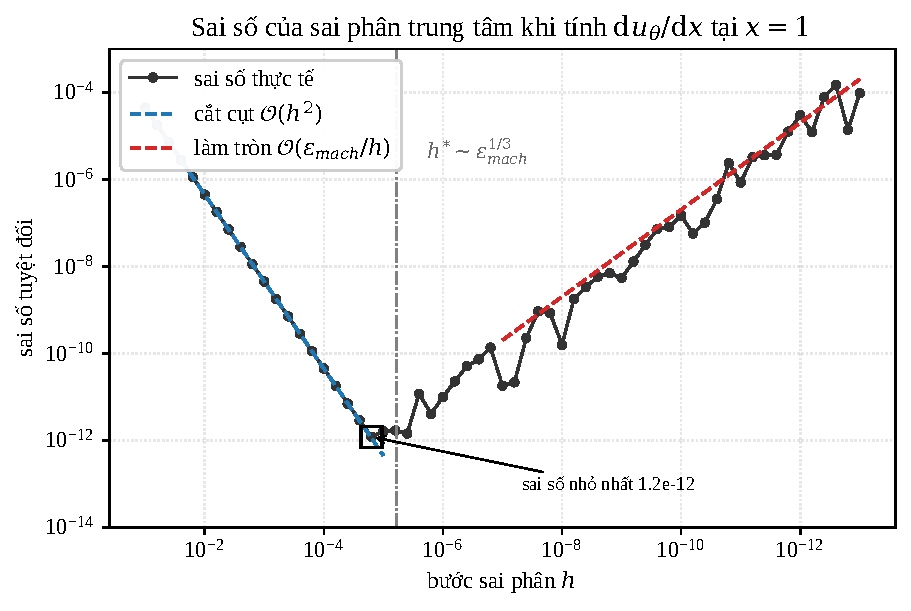
\includegraphics[width=0.82\textwidth]{Images/chap_3/hinh_saiphan.pdf}
\caption{Sai số tuyệt đối của sai phân trung tâm khi tính
$\mathrm{d}\Net_{\btheta}/\mathrm{d}x$ tại $x=1$, thang log--log, trục hoành
hướng về phía $h$ nhỏ dần. Đường gạch màu xanh là tiệm cận cắt cụt
$\mathcal{O}(h^2)$, đường gạch màu đỏ là tiệm cận làm tròn
$\mathcal{O}(\eps/h)$. Không có cách chọn $h$ nào đưa sai số xuống dưới đáy hình
chữ V; vi phân tự động cho giá trị chính xác tới độ chính xác máy.}
\label{fig:saiphan}
\end{figure}
 
\begin{nhanxet}[Hệ quả đối với bài toán phương trình vi phân]
\label{nx:fd-pde}
Bảng~\ref{tab:fd-error} mới chỉ là đạo hàm bậc nhất. Ba lý do khiến tình hình xấu
đi nhanh chóng trong bối cảnh của báo cáo.
 
Thứ nhất, với đạo hàm bậc hai, lược đồ trung tâm
$\big(f(x+h)-2f(x)+f(x-h)\big)/h^2$ có sai số cắt cụt $\mathcal{O}(h^2)$ nhưng
sai số làm tròn $\mathcal{O}(\eps|f|/h^2)$; lặp lại lập luận của
Mệnh đề~\ref{md:fd-rao-can} cho $h^{*} \sim \eps^{1/4}$ và sai số tốt nhất chỉ
còn cỡ $\eps^{1/2} \approx 10^{-8}$. Mỗi bậc đạo hàm làm mất thêm vài bậc độ
chính xác.
 
Thứ hai, với miền $n_0$ chiều, mỗi đạo hàm riêng cần thêm hai lần đánh giá mạng,
nên chi phí nhân lên tuyến tính theo $n_0$ -- trong khi vi phân tự động cho toàn
bộ gradient trong một lượt.
 
Thứ ba, và quan trọng nhất: phần dư $\mathcal{L}[\Net_{\btheta}] - f$ được đưa
\emph{trực tiếp} vào hàm mục tiêu rồi lại được lấy đạo hàm theo $\btheta$. Sai số
$10^{-8}$ ở phần dư không chỉ làm hàm mục tiêu sai lệch, nó còn tạo ra một
gradient sai lệch mà thuật toán tối ưu sẽ trung thành đi theo. Nói cách khác, sai
số xấp xỉ ở bước này không bị dập tắt mà được khuếch đại qua toàn bộ quá trình
huấn luyện, và nó đặt một sàn cứng lên độ chính xác cuối cùng của nghiệm. Đây là
lý do vì sao phương pháp PINN ở Chương~\ref{chap:pinn} bắt buộc dùng vi phân tự
động; Raissi và cộng sự~\cite{raissi2019} nêu điều này như một điều kiện của
phương pháp chứ không phải một lựa chọn cài đặt.
\end{nhanxet}
 
\subsection{Chế độ thuận}
\label{subsec:forward-mode}
 
Xét hàm $f : \R^n \to \R^m$ được tính bởi dãy phép toán sơ cấp $v_1,\dots,v_K$
theo đồ thị của Định nghĩa~\ref{def:comp-graph}. Cố định một \emph{vectơ mầm}
(seed) $\bm{r} \in \R^n$. \emph{Chế độ thuận} gắn kèm mỗi biến $v_k$ một
\emph{đạo hàm thuận} (tangent)
\begin{equation}
\dot{v}_k \coloneqq \frac{\partial v_k}{\partial \bx}\, \bm{r},
\label{eq:tangent}
\end{equation}
tức đạo hàm có hướng của $v_k$ theo hướng $\bm{r}$, rồi lan truyền $\dot{v}_k$
\emph{cùng chiều} với lượt tính giá trị, theo quy tắc dây chuyền
\begin{equation}
\dot{v}_k = \sum_{j \in \mathrm{Pa}(k)}
  \frac{\partial \varphi_k}{\partial v_j}\, \dot{v}_j ,
\qquad
\dot{\bx} = \bm{r}.
\label{eq:forward-truy-hoi}
\end{equation}
Kết thúc lượt, $\dot{\bm{y}} = \D f(\bx)\,\bm{r}$: một lượt chế độ thuận cho ta
\emph{tích Jacobi--vectơ} (Jacobian--vector product, JVP). Muốn có toàn bộ ma
trận Jacobi $m\times n$, cần $n$ lượt với $\bm{r} = \bm{e}_1,\dots,\bm{e}_n$. Vậy
chế độ thuận \emph{hiệu quả khi $n \ll m$}.
 
Cách phát biểu cô đọng nhất của \eqref{eq:forward-truy-hoi} là qua số đối ngẫu.
 
\begin{definition}[Số đối ngẫu]
\label{def:doi-ngau}
Vành số đối ngẫu là $\mathbb{D} = \{ a + b\epsilon : a,b \in \R \}$ với phép
cộng và nhân thông thường cùng quy tắc $\epsilon^2 = 0$, $\epsilon \neq 0$.
\end{definition}
 
\begin{bode}[Nguyên lý của chế độ thuận]
\label{bd:doi-ngau}
Nếu $f$ khả vi tại $a$ thì, trong $\mathbb{D}$,
\begin{equation}
f(a + b\epsilon) = f(a) + f'(a)\, b\, \epsilon .
\label{eq:doi-ngau}
\end{equation}
\end{bode}
 
\begin{proof}
Với $f$ đa thức, khai triển $(a+b\epsilon)^k = a^k + k a^{k-1}b\epsilon$ theo
nhị thức Newton: mọi số hạng chứa $\epsilon^2$ trở lên đều triệt tiêu do
$\epsilon^2 = 0$. Lấy tổ hợp tuyến tính cho \eqref{eq:doi-ngau} với $f$ đa thức.
Với $f$ tổng quát khả vi, \eqref{eq:doi-ngau} được \emph{lấy làm định nghĩa} của
phép mở rộng $f$ lên $\mathbb{D}$; định nghĩa này nhất quán với phép hợp thành,
vì
\[
(g\circ f)(a+b\epsilon) = g\big(f(a) + f'(a)b\,\epsilon\big)
 = g(f(a)) + g'(f(a))f'(a)\,b\,\epsilon,
\]
đúng bằng quy tắc dây chuyền.
\end{proof}
 
Bổ đề~\ref{bd:doi-ngau} cho một cài đặt ngắn gọn đến bất ngờ: chỉ cần \emph{nạp
chồng} các phép toán số học cho kiểu số đối ngẫu rồi đánh giá $f$ tại
$x + 1\cdot\epsilon$; phần $\epsilon$ của kết quả chính là $f'(x)$, chính xác,
không cần chọn $h$. Toàn bộ vấn đề của Mệnh đề~\ref{md:fd-rao-can} biến mất, vì
ở đây không có phép trừ hai số gần nhau nào cả.
 
\subsection{Chế độ ngược}
\label{subsec:reverse-mode}
 
Đối ngẫu với chế độ thuận, \emph{chế độ ngược} cố định một vectơ mầm
$\bm{w} \in \R^m$ ở phía đầu ra và gắn kèm mỗi biến một \emph{biến liên hợp}
(adjoint)
\begin{equation}
\bar{v}_k \coloneqq \frac{\partial \big(\bm{w}^{\top} f\big)}{\partial v_k},
\label{eq:adjoint}
\end{equation}
rồi lan truyền chúng \emph{ngược chiều} đồ thị theo \eqref{eq:chain-graph}. Kết
thúc lượt, $\bar{\bx} = \bm{w}^{\top}\D f(\bx)$: một lượt cho ta tích
vectơ--Jacobi \eqref{eq:vjp}. Cần $m$ lượt để có toàn bộ Jacobi, nên chế độ ngược
\emph{hiệu quả khi $m \ll n$}.
 
\begin{nhanxet}
\label{nx:bp-is-reverse}
Lan truyền ngược ở Mục~\ref{sec:backprop} chính là chế độ ngược áp dụng cho
trường hợp $m = 1$ (hàm mục tiêu vô hướng, $\bm{w} = 1$) và $n = P$ (số tham
số). Đây là kịch bản cực đoan nhất về tỉ lệ $m/n$, và cũng là lý do khiến chế độ
ngược thống trị trong học sâu. Mối liên hệ này giải thích vì sao mọi thư viện
hiện đại~\cite{paszke2019} chỉ cài đặt một cơ chế vi phân tự động chung, còn
``lan truyền ngược'' chỉ là tên gọi lịch sử của một trường hợp riêng. Nó cũng
giải thích vì sao Mệnh đề~\ref{md:bp}, dù được chứng minh riêng cho mạng truyền
thẳng, không cần chứng minh lại khi ta thêm phần dư phương trình vi phân vào đồ
thị.
\end{nhanxet}
 
\begin{dinhly}[Nguyên lý gradient rẻ]
\label{dl:cheap-gradient}
Với mọi hàm $f:\R^n \to \R$ được tính bởi một chương trình gồm các phép toán sơ
cấp, chế độ ngược tính $\nabla f$ với số phép toán không vượt quá một hằng số
nhân với số phép toán đánh giá $f$, và hằng số ấy \emph{không phụ thuộc $n$}.
\end{dinhly}
 
Giá trị chính xác của hằng số phụ thuộc mô hình chi phí được dùng; các chặn
thường được trích dẫn nằm trong khoảng $3$ đến $5$~\cite{griewank2008}.
Mệnh đề~\ref{md:chi-phi-bp} là trường hợp riêng của
Định lý~\ref{dl:cheap-gradient} cho mạng truyền thẳng, ở đó ta tính được hằng số
cụ thể $c \le 3$ nhờ biết rõ cấu trúc đồ thị.
 
Đánh đổi là bộ nhớ: chế độ ngược phải lưu (hoặc tính lại) mọi giá trị trung gian
của lượt thuận, nên chi phí bộ nhớ tỉ lệ với \emph{độ dài} của đồ thị tính toán.
Điều này trở nên đáng kể khi ta lấy đạo hàm bậc cao ở mục sau.
 
\begin{table}[htbp]
\centering
\caption{So sánh hai chế độ vi phân tự động cho $f:\R^n\to\R^m$.}
\label{tab:ad-modes}
\begin{tabular}{@{}lll@{}}
\toprule
 & Chế độ thuận & Chế độ ngược \\
\midrule
Đại lượng lan truyền   & tangent $\dot{v}$          & adjoint $\bar{v}$ \\
Chiều lan truyền       & cùng chiều đồ thị          & ngược chiều đồ thị \\
Một lượt cho ta        & $\D f\,\bm{r}$ (JVP)       & $\bm{w}^{\top}\D f$ (VJP) \\
Số lượt cho Jacobi đầy & $n$                        & $m$ \\
Hiệu quả khi           & $n \ll m$                  & $m \ll n$ \\
Bộ nhớ                 & $\mathcal{O}(1)$ theo độ dài đồ thị
                       & $\mathcal{O}(\text{độ dài đồ thị})$ \\
\bottomrule
\end{tabular}
\end{table}
 
\subsection{Đạo hàm theo biến đầu vào và đạo hàm bậc cao}
\label{subsec:bac-cao-ad}
 
Đây là mục có ý nghĩa quyết định đối với phần còn lại của báo cáo, và là mắt
xích nối trở lại Chương~\ref{chap:fnn}. Khi giải phương trình vi phân, mạng
$\Net_{\btheta}(\bx)$ đóng vai trò hàm thử và ta cần các đại lượng
$\partial_{x_i}\Net_{\btheta}$, $\partial^2_{x_ix_j}\Net_{\btheta}$, sau đó lại
phải lấy đạo hàm của toàn bộ biểu thức ấy theo $\btheta$.
 
Điểm mấu chốt là: \emph{đầu ra của một lượt vi phân tự động cũng là một hàm được
tính bởi một đồ thị tính toán}. Do đó có thể áp dụng vi phân tự động lên chính
nó. Mệnh đề sau làm rõ rằng cơ chế này không phải một thủ thuật lập trình mà tái
tạo đúng các hệ thức truy hồi đã được chứng minh ở Chương~\ref{chap:fnn}.
 
\begin{menhde}[Vi phân tự động tái tạo các truy hồi \eqref{eq:G-truy-hoi} và
\eqref{eq:S-truy-hoi}]
\label{md:ad-tai-tao}
Xét mạng theo Định nghĩa~\ref{def:fnn} với $\sigma \in C^2$ và $n_L = 1$.
 
\emph{(a)} Một lượt chế độ thuận trên đồ thị của lượt xuôi, với vectơ mầm
$\dot{\bx} = \bm{r}$, sinh ra dãy tangent $\dot{\ba}^{(\ell)}$ thoả đúng
\begin{equation}
\dot{\ba}^{(\ell)} = \bD^{(\ell)}\bW^{(\ell)}\dot{\ba}^{(\ell-1)},
\qquad \dot{\ba}^{(0)} = \bm{r},
\label{eq:ad-jvp}
\end{equation}
tức $\dot{\ba}^{(\ell)} = \bG^{(\ell)}\bm{r}$ với $\bG^{(\ell)}$ của
Mệnh đề~\ref{md:jacobian}. Do đó $n_0$ lượt thuận với các mầm
$\bm{e}_1,\dots,\bm{e}_{n_0}$ cho đúng ma trận $\partial_{\bx}\Net_{\btheta}$
của \eqref{eq:jacobian}.
 
\emph{(b)} Một lượt chế độ thuận với mầm $\bm{r}$ áp lên đồ thị \emph{mở rộng}
đã chứa $\dot{\ba}^{(\ell)}$ (tức chế độ thuận trên chế độ thuận) sinh ra dãy
$\ddot{\ba}^{(\ell)}$ thoả
\begin{equation}
\ddot{a}^{(\ell)}_k
 = \sigma''\!\big(z^{(\ell)}_k\big)\big(\dot{z}^{(\ell)}_k\big)^2
 + \sigma'\!\big(z^{(\ell)}_k\big)
   \sum_{j} w^{(\ell)}_{kj}\,\ddot{a}^{(\ell-1)}_j,
\qquad \ddot{\ba}^{(0)} = \bm{0},
\label{eq:ad-hvp}
\end{equation}
tức $\ddot{a}^{(\ell)}_k = \bm{r}^{\top}\bS^{(\ell)}_k\bm{r}$ với
$\bS^{(\ell)}_k$ của Mệnh đề~\ref{md:hessian}. Nói riêng, mỗi lượt như vậy cho
\emph{một dạng toàn phương} $\bm{r}^{\top}\nabla^2_{\bx}\Net_{\btheta}\,\bm{r}$
của Hessian, và với $\bm{r} = \bm{e}_i$ ta được đúng
$\partial^2_{x_i x_i}\Net_{\btheta}$.
\end{menhde}
 
\begin{proof}
\emph{(a)} Áp dụng \eqref{eq:forward-truy-hoi} cho hai phép toán sơ cấp của lớp
$\ell$. Với phép affine \eqref{eq:fnn-affine}, các đỉnh cha của $\bz^{(\ell)}$ là
$\ba^{(\ell-1)}$ (cùng $\bW^{(\ell)},\bb^{(\ell)}$, vốn có tangent bằng $0$ vì
$\btheta$ không phụ thuộc $\bx$), và
$\partial\bz^{(\ell)}/\partial\ba^{(\ell-1)} = \bW^{(\ell)}$, cho
$\dot{\bz}^{(\ell)} = \bW^{(\ell)}\dot{\ba}^{(\ell-1)}$. Với phép kích hoạt
\eqref{eq:fnn-act}, Jacobi là $\bD^{(\ell)}$, cho
$\dot{\ba}^{(\ell)} = \bD^{(\ell)}\dot{\bz}^{(\ell)}$. Ghép hai bước được
\eqref{eq:ad-jvp}, trùng với \eqref{eq:G-truy-hoi} nhân phải với $\bm{r}$. Quy
nạp theo $\ell$ với cơ sở $\dot{\ba}^{(0)} = \bm{r} = \bG^{(0)}\bm{r}$ cho
$\dot{\ba}^{(\ell)} = \bG^{(\ell)}\bm{r}$.
 
\emph{(b)} Lấy đạo hàm có hướng theo $\bm{r}$ của hai hệ thức trong \emph{(a)}.
Với phép affine, $\ddot{\bz}^{(\ell)} = \bW^{(\ell)}\ddot{\ba}^{(\ell-1)}$, tức
$\ddot{z}^{(\ell)}_k = \sum_j w^{(\ell)}_{kj}\ddot{a}^{(\ell-1)}_j$. Với phép
kích hoạt, $\dot{a}^{(\ell)}_k = \sigma'(z^{(\ell)}_k)\dot{z}^{(\ell)}_k$ là
tích của hai đại lượng cùng phụ thuộc $\bx$, nên quy tắc tích cho
\[
\ddot{a}^{(\ell)}_k
 = \sigma''\!\big(z^{(\ell)}_k\big)\big(\dot z^{(\ell)}_k\big)^2
 + \sigma'\!\big(z^{(\ell)}_k\big)\,\ddot{z}^{(\ell)}_k ,
\]
đúng bằng \eqref{eq:ad-hvp}. Để nhận ra đây là dạng toàn phương của
$\bS^{(\ell)}_k$, nhân hai vế của \eqref{eq:S-truy-hoi} với $\bm{r}^{\top}$ bên
trái và $\bm{r}$ bên phải: số hạng thứ nhất cho
$\sigma''(z^{(\ell)}_k)\big(\bm{g}^{(\ell)}_k\bm{r}\big)^2$, và
$\bm{g}^{(\ell)}_k\bm{r} = \dot z^{(\ell)}_k$ theo \emph{(a)}; số hạng thứ hai
cho $\sigma'(z^{(\ell)}_k)\sum_j w^{(\ell)}_{kj}\,
\bm{r}^{\top}\bS^{(\ell-1)}_j\bm{r}$. Hai vế thoả cùng một truy hồi với cùng điều
kiện đầu ($\bS^{(0)}_k = \bm{0}$ và $\ddot{\ba}^{(0)} = \bm{0}$), nên trùng nhau
theo quy nạp.
\end{proof}
 
\begin{nhanxet}[Ý nghĩa của Mệnh đề~\ref{md:ad-tai-tao}]
Ba kết luận thực hành.
 
Thứ nhất, người dùng \emph{không phải lập trình} $\sigma''$: thư viện chỉ biết
đạo hàm của các phép toán sơ cấp và tự sinh ra số hạng $\sigma''(z_k)\dot z_k^2$
qua quy tắc tích. Đây là điểm khác biệt căn bản với
Thuật toán~\ref{alg:dao-ham}, vốn đòi hỏi viết tường minh công thức
\eqref{eq:tanh-d2}.
 
Thứ hai, mỗi lượt cho một dạng toàn phương chứ không phải toàn bộ Hessian. Muốn
đủ $\nabla^2_{\bx}\Net_{\btheta}$ cần $\mathcal{O}(n_0)$ lượt (hoặc
$\mathcal{O}(n_0^2)$ nếu lấy từng phần tử riêng lẻ), khớp với ước lượng chi phí ở
Nhận xét~\ref{nx:chi-phi-hessian}. Với phương trình Laplace hay khuếch tán, thứ
cần thiết là \emph{vết} $\sum_i \partial^2_{x_ix_i}\Net_{\btheta}$, tức $n_0$
lượt với các mầm $\bm{e}_i$ -- không cần Hessian đầy đủ.
 
Thứ ba, đây là kết quả về \emph{tính đúng đắn}, không phải về chiến lược cài đặt
tối ưu. Trong PyTorch, cách thông dụng là dùng chế độ ngược hai lần thay vì chế
độ thuận hai lần; hai cách cho cùng kết quả nhưng khác nhau về chi phí bộ nhớ.
\end{nhanxet}
 
\paragraph{Ba lượt của một bước huấn luyện PINN.}
Với phương trình $u_t = \nu u_{xx}$, một bước huấn luyện gồm:
\begin{enumerate}[label=(\arabic*), leftmargin=*]
\item Lượt thứ nhất (chế độ ngược, \emph{giữ lại} đồ thị) cho $\partial_x
      \Net_{\btheta}$ và $\partial_t\Net_{\btheta}$ như những đỉnh mới trong đồ
      thị mở rộng.
\item Lượt thứ hai áp lên $\partial_x\Net_{\btheta}$ cho
      $\partial^2_{xx}\Net_{\btheta}$, từ đó dựng phần dư
      $\mathcal{R} = \partial_t\Net_{\btheta} - \nu\,\partial^2_{xx}
      \Net_{\btheta}$ và hàm mục tiêu $J$.
\item Lượt thứ ba lấy $\nabla_{\btheta} J$ trên toàn bộ đồ thị mở rộng, phục vụ
      bước cập nhật tối ưu.
\end{enumerate}
Trong PyTorch~\cite{paszke2019}, hai lượt đầu tương ứng với việc gọi
\texttt{torch.autograd.grad(u, x, create\_graph=True)}, trong đó cờ
\texttt{create\_graph} báo cho hệ thống rằng bản thân phép tính gradient phải được
\emph{ghi lại} vào băng ghi thay vì bị loại bỏ sau khi dùng. Bỏ sót cờ này là lỗi
cài đặt phổ biến nhất khi triển khai PINN: chương trình vẫn chạy, hàm mục tiêu
vẫn được tính, nhưng $\nabla_{\btheta} J$ bỏ mất toàn bộ đóng góp đi qua phần dư,
và mạng học ra một hàm không liên quan đến phương trình.
 
\begin{nhanxet}[Chi phí của đạo hàm bậc cao]
\label{nx:chi-phi-bac-cao}
Mỗi bậc đạo hàm nhân độ dài đồ thị lên một hằng số. Với phương trình bậc hai như
phương trình khuếch tán hay Burgers, đồ thị dùng cho lượt tối ưu hoá dài gấp
khoảng bốn đến sáu lần đồ thị của lượt xuôi thuần tuý, và bộ nhớ tăng theo cùng
tỉ lệ do Định lý~\ref{dl:cheap-gradient} đòi hỏi lưu toàn bộ giá trị trung gian.
Ước lượng ``bốn đến sáu'' ở đây là ước lượng \emph{a priori}, và phép đo ở
Mục~\ref{sec:tn9} cho thấy nó \emph{thấp}: bội số đo được là khoảng chín. Sai
lệch nằm ở chỗ ước lượng này ngầm coi hai bậc đạo hàm tốn như nhau, trong khi
lượt lấy $\partial_{xx}u$ chạy ngược trên đồ thị đã được lượt lấy
$\partial_{x}u$ nối dài; xem phần thảo luận ở Mục~\ref{sec:tn9}.
Đây là nguyên nhân chính khiến một bước huấn luyện PINN đắt hơn đáng kể so với
một bước huấn luyện mạng hồi quy cùng kích thước, và là lý do phải chọn hàm kích
hoạt trơn: với ReLU, $\sigma'' \equiv 0$ hầu khắp nơi
(Hệ quả~\ref{hq:relu-hkn}), số hạng thứ nhất của \eqref{eq:ad-hvp} triệt tiêu ở
mọi lớp, và theo Hệ quả~\ref{hq:pinn-hong} hàm mục tiêu trở thành hằng số địa
phương.
\end{nhanxet}
 
\begin{nhanxet}[Kết hợp hai chế độ]
Khi cần tích Hessian--vectơ $\nabla^2_{\btheta} J(\btheta)\,\bm{r}$ -- đại lượng
xuất hiện trong các phương pháp Newton chặt cụt -- cách hiệu quả nhất là
\emph{thuận trên ngược}: áp dụng chế độ thuận lên đồ thị của lượt ngược. Lý do
nằm ở Bảng~\ref{tab:ad-modes}: lượt ngược cho hàm
$\btheta \mapsto \nabla_{\btheta}J \in \R^P$, và ta chỉ cần JVP của hàm này theo
một hướng, tức đúng việc mà chế độ thuận làm trong một lượt. Chi phí do đó chỉ
tương đương một vài lần đánh giá $J$, thay vì $\mathcal{O}(P^2)$ nếu dựng tường
minh Hessian.
\end{nhanxet}
 
%==============================================================================
\section{Các thuật toán tối ưu}
\label{sec:optimizers}
%==============================================================================
 
\subsection{Đặc thù của bài toán}
\label{subsec:dac-thu}
 
Bài toán \eqref{eq:erm} có ba đặc điểm quy định việc lựa chọn thuật toán, và cả
ba đều đã được thiết lập ở các chương trước chứ không phải giả định.
 
\emph{Không lồi.} Mệnh đề~\ref{md:khong-loi} cho thấy $J$ không lồi do đối xứng
dấu, và Nhận xét~\ref{nx:doi-xung-hoan-vi} cho thấy mỗi cực tiểu sinh ra ít nhất
$2^{n_1}n_1!$ cực tiểu tương đương. Ta chỉ có thể kỳ vọng tìm được \emph{điểm
dừng}, không phải cực tiểu toàn cục.
 
\emph{Chiều rất lớn.} $P$ cho bởi \eqref{eq:so-tham-so} thường ở mức $10^3$ đến
$10^7$, nên mọi phương pháp cần lưu ma trận $P\times P$ đều bị loại ngay.
 
\emph{Điều kiện xấu.} Trong bối cảnh phương trình vi phân, hàm mục tiêu
\eqref{eq:pinn-loss} tổ hợp nhiều thành phần có thứ nguyên và thang độ khác nhau
-- phần dư phương trình, điều kiện biên, điều kiện ban đầu -- tạo ra một Hessian
có số điều kiện lớn.
 
Mọi thuật toán dưới đây đều thuộc lược đồ lặp chung
\begin{equation}
\btheta_{k+1} = \btheta_k + \alpha_k \bm{p}_k,
\label{eq:iter-scheme}
\end{equation}
và chỉ khác nhau ở cách chọn \emph{hướng} $\bm{p}_k$ và \emph{độ dài bước}
$\alpha_k$~\cite{nocedal2006}.
 
\subsection{Hạ gradient và hạ gradient ngẫu nhiên}
\label{subsec:sgd}
 
Lựa chọn đơn giản nhất là $\bm{p}_k = -\nabla J(\btheta_k)$, hướng giảm nhanh
nhất tại chỗ. Với $N$ lớn, việc tính đủ tổng trong \eqref{eq:erm} ở mỗi bước quá
tốn kém, nên ta thay bằng ước lượng không chệch trên một lô nhỏ
$\mathcal{B}_k \subset \{1,\dots,N\}$:
\begin{equation}
\bm{g}_k = \frac{1}{|\mathcal{B}_k|}\sum_{i \in \mathcal{B}_k}
\nabla_{\btheta}\, \varrho\!\left(\Net_{\btheta_k}(\bx_i), \bm{y}_i\right),
\qquad
\btheta_{k+1} = \btheta_k - \alpha_k \bm{g}_k .
\label{eq:sgd}
\end{equation}
Trình bày về hạ gradient ngẫu nhiên và các biến thể của nó ở mục này theo
Goodfellow và cộng sự~\cite{goodfellow2016}.
 
\begin{dinhly}[Hội tụ dưới điều kiện bước học Robbins--Monro]
\label{dl:robbins-monro}
Giả sử $J$ khả vi liên tục, bị chặn dưới, $\nabla J$ Lipschitz, ước lượng
$\bm{g}_k$ không chệch và có phương sai bị chặn. Nếu dãy bước học thoả mãn
\begin{equation}
\sum_{k=1}^{\infty} \alpha_k = \infty,
\qquad
\sum_{k=1}^{\infty} \alpha_k^2 < \infty,
\label{eq:rm}
\end{equation}
thì $J(\btheta_k)$ hội tụ hầu chắc chắn và
$\liminf_{k\to\infty}\|\nabla J(\btheta_k)\| = 0$ hầu chắc chắn.
\end{dinhly}
 
Hai điều kiện trong \eqref{eq:rm} có ý nghĩa đối lập và đều cần thiết. Điều kiện
thứ nhất bảo đảm thuật toán có thể đi được quãng đường tuỳ ý -- nếu
$\sum\alpha_k < \infty$ thì $\btheta_k$ bị nhốt trong một hình cầu quanh
$\btheta_0$ và không thể tới nghiệm nếu nghiệm nằm ngoài. Điều kiện thứ hai bảo
đảm nhiễu ngẫu nhiên bị dập tắt dần. Cặp điều kiện này xuất phát từ Robbins và
Monro trong bài toán tìm nghiệm ngẫu nhiên; phát biểu cho trường hợp không lồi
như trên thuộc về Bertsekas và Tsitsiklis~\cite{bertsekas2000}.
 
Trong thực hành, người ta hiếm khi dùng dãy $\alpha_k$ thoả \eqref{eq:rm} một
cách nghiêm ngặt, mà dùng bước học hằng số theo từng giai đoạn rồi giảm dần theo
lịch. Mệnh đề sau lượng hoá cái giá phải trả cho sự thoả hiệp đó.
 
\begin{menhde}[Sàn nhiễu của bước học hằng số]
\label{md:san-nhieu}
Xét mô hình bậc hai một chiều $J(\theta) = \tfrac{\mu}{2}\theta^2$ với $\mu > 0$,
và bước lặp \eqref{eq:sgd} với bước học hằng số $\alpha \in (0, 2/\mu)$ và
gradient nhiễu $g_k = \mu\theta_k + \xi_k$, trong đó $\xi_k$ độc lập, kỳ vọng
$0$, phương sai $\varsigma^2$. Khi đó
\begin{equation}
\lim_{k\to\infty}\E\big[\theta_k^2\big]
 = \frac{\alpha\,\varsigma^{2}}{\mu\,(2-\alpha\mu)},
\qquad
\lim_{k\to\infty}\E\big[J(\theta_k)\big]
 = \frac{\alpha\,\varsigma^{2}}{2\,(2-\alpha\mu)},
\label{eq:san-nhieu}
\end{equation}
và do đó $\lim_{k\to\infty}\E[J(\theta_k)] \sim \alpha\varsigma^{2}/4$ khi
$\alpha \to 0^{+}$.
\end{menhde}
 
\begin{proof}
Thay $g_k$ vào \eqref{eq:sgd}:
$\theta_{k+1} = (1-\alpha\mu)\theta_k - \alpha\xi_k$. Đặt
$s_k = \E[\theta_k^2]$. Vì $\xi_k$ độc lập với $\theta_k$ và có kỳ vọng $0$, số
hạng chéo triệt tiêu khi bình phương và lấy kỳ vọng:
\[
s_{k+1} = (1-\alpha\mu)^2 s_k + \alpha^2\varsigma^2 .
\]
Đây là truy hồi affine với hệ số $q := (1-\alpha\mu)^2 \in [0,1)$ khi
$\alpha \in (0,2/\mu)$, nên $s_k$ hội tụ tới điểm bất động
$s_\infty = \alpha^2\varsigma^2/(1-q)$. Khai triển
$1 - q = 2\alpha\mu - \alpha^2\mu^2 = \alpha\mu(2-\alpha\mu)$ cho
\eqref{eq:san-nhieu}. Đẳng thức thứ hai theo $J = \tfrac{\mu}{2}\theta^2$.
\end{proof}
 
\begin{nhanxet}[Sàn nhiễu]
\label{nx:noise-floor}
Mệnh đề~\ref{md:san-nhieu} cho một kết luận sắc nét: với bước học hằng số, dãy
$\btheta_k$ \emph{không} hội tụ tới điểm dừng mà chỉ dao động trong một lân cận,
và giá trị kỳ vọng của hàm mục tiêu bị chặn dưới bởi một mức tỉ lệ \emph{tuyến
tính} với $\alpha$ và với phương sai của gradient. Muốn giảm sàn nhiễu mười lần,
phải giảm bước học mười lần, và khi ấy tốc độ tiến tới lân cận cũng chậm đi
tương ứng -- hệ số co là $(1-\alpha\mu)$.
 
Hiện tượng này là giới hạn cơ bản của mọi phương pháp ngẫu nhiên bậc nhất, không
phải một khiếm khuyết cài đặt, và nó là lập luận trung tâm ở
Mục~\ref{subsec:adam-vs-lbfgs}. Cần nói rõ phạm vi: mệnh đề được chứng minh cho
mô hình bậc hai một chiều, tức là một mô hình địa phương quanh điểm cực tiểu, chứ
không phải cho hàm mục tiêu PINN đầy đủ. Nó giải thích hiện tượng chững lại quan
sát được ở Hình~\ref{fig:hoitu}, nhưng không phải là một định lý về hàm mục tiêu
ấy.
\end{nhanxet}
 
\subsection{Động lượng}
\label{subsec:momentum}
 
Hạ gradient thuần tuý tiến rất chậm trong các ``khe hẹp'' của hàm mục tiêu: nó
dao động qua lại theo hướng có độ cong lớn và bò rất chậm theo hướng có độ cong
nhỏ. Phương pháp \emph{động lượng}~\cite{goodfellow2016} khắc phục bằng cách tích
luỹ một trung bình trượt của các gradient quá khứ:
\begin{equation}
\bm{v}_k = \beta \bm{v}_{k-1} - \alpha \bm{g}_k,
\qquad
\btheta_{k+1} = \btheta_k + \bm{v}_k,
\qquad \beta \in [0,1).
\label{eq:momentum}
\end{equation}
 
\begin{bode}[Hệ số khuếch đại của động lượng]
\label{bd:momentum}
Giả sử $\bm{g}_k \equiv \bm{g}$ không đổi và $\bm{v}_0 = \bm{0}$. Khi đó
\begin{equation}
\bm{v}_k = -\alpha\,\frac{1-\beta^{k}}{1-\beta}\,\bm{g}
\;\xrightarrow[k\to\infty]{}\;
-\frac{\alpha}{1-\beta}\,\bm{g}.
\label{eq:momentum-khuech-dai}
\end{equation}
Ngược lại, nếu $\bm{g}_k$ đổi dấu luân phiên, $\bm{g}_k = (-1)^k\bm{g}$, thì
\begin{equation}
\bm{v}_k = -\alpha\,(-1)^{k}\,\frac{1-(-\beta)^{k}}{1+\beta}\,\bm{g},
\qquad\text{nên}\qquad
\norm{\bm{v}_k} \;\xrightarrow[k\to\infty]{}\;
  \frac{\alpha\,\norm{\bm{g}}}{1+\beta},
\label{eq:momentum-dao-dong}
\end{equation}
tức biên độ bị \emph{thu nhỏ} đi thừa số $1/(1+\beta)$ (bản thân $\bm{v}_k$ không
hội tụ, nó dao động đổi dấu theo $k$).
\end{bode}
 
\begin{proof}
Khai triển truy hồi \eqref{eq:momentum}:
$\bm{v}_k = -\alpha\sum_{j=0}^{k-1}\beta^{j}\bm{g}_{k-j}$. Với $\bm{g}_k \equiv
\bm{g}$, tổng là cấp số nhân $\sum_{j=0}^{k-1}\beta^j = (1-\beta^k)/(1-\beta)$,
cho \eqref{eq:momentum-khuech-dai}. Với $\bm{g}_{k-j} = (-1)^{k-j}\bm{g}
= (-1)^{k}(-1)^{j}\bm{g}$, tổng trở thành
$(-1)^k\sum_{j=0}^{k-1}(-\beta)^{j} = (-1)^k\,\dfrac{1-(-\beta)^{k}}{1+\beta}$,
cho \eqref{eq:momentum-dao-dong}; vì $|\beta| < 1$ nên $(-\beta)^k \to 0$ và
chuẩn của $\bm{v}_k$ hội tụ tới $\alpha\norm{\bm{g}}/(1+\beta)$.
\end{proof}
 
Bổ đề~\ref{bd:momentum} giải thích chính xác cơ chế của động lượng: thành phần
\emph{nhất quán} của gradient được khuếch đại lên $1/(1-\beta)$ lần, còn thành
phần \emph{dao động} bị nén xuống $1/(1+\beta)$ lần. Với $\beta = 0{,}9$, tỉ số
giữa hai hệ số là $(1+\beta)/(1-\beta) = 19$: động lượng làm tăng độ tương phản
giữa hướng có ích và hướng dao động lên gần hai mươi lần. Biến thể
\emph{Nesterov} đánh giá gradient tại điểm đã được đẩy tới trước,
$\btheta_k + \beta\bm{v}_{k-1}$, tạo hiệu ứng ``nhìn trước'' giúp giảm vọt lố khi
tới gần điểm cực tiểu.
 
\subsection{Phương pháp thích nghi và thuật toán Adam}
\label{subsec:adam}
 
Ý tưởng tiếp theo là dùng bước học \emph{riêng cho từng toạ độ}, tự động thu nhỏ
ở những hướng có gradient lớn kéo dài. AdaGrad tích luỹ toàn bộ lịch sử bình
phương gradient, nên bước học giảm đơn điệu và có thể tắt quá sớm; RMSProp thay
tổng tích luỹ bằng trung bình trượt hàm mũ, khắc phục nhược điểm
đó~\cite{goodfellow2016}. Adam kết hợp
RMSProp với động lượng, đồng thời hiệu chỉnh độ chệch của các trung bình trượt ở
những bước đầu~\cite{kingma2015}.
 
\begin{algorithm}[htbp]
\caption{Adam}
\label{alg:adam}
\begin{algorithmic}[1]
\Require Bước học $\alpha$, hệ số $\beta_1,\beta_2 \in [0,1)$, hằng số
  $\varepsilon > 0$, tham số ban đầu $\btheta_0$
\State $\bm{m}_0 \gets \bm{0}$, \quad $\bm{v}_0 \gets \bm{0}$, \quad $k \gets 0$
\While{chưa thoả tiêu chuẩn dừng}
  \State $k \gets k+1$
  \State $\bm{g}_k \gets \nabla_{\btheta} J_{\mathcal{B}_k}(\btheta_{k-1})$
  \State $\bm{m}_k \gets \beta_1 \bm{m}_{k-1} + (1-\beta_1)\bm{g}_k$
    \Comment{mô-men bậc nhất}
  \State $\bm{v}_k \gets \beta_2 \bm{v}_{k-1}
    + (1-\beta_2)\, \bm{g}_k \odot \bm{g}_k$
    \Comment{mô-men bậc hai}
  \State $\hat{\bm{m}}_k \gets \bm{m}_k / (1-\beta_1^{\,k})$
    \Comment{hiệu chỉnh độ chệch, Bổ đề~\ref{bd:adam-bias}}
  \State $\hat{\bm{v}}_k \gets \bm{v}_k / (1-\beta_2^{\,k})$
  \State $\btheta_k \gets \btheta_{k-1} - \alpha\, \hat{\bm{m}}_k \big/
    \left(\sqrt{\hat{\bm{v}}_k} + \varepsilon\right)$
\EndWhile
\State \Return $\btheta_k$
\end{algorithmic}
\end{algorithm}
 
\begin{bode}[Vì sao cần hiệu chỉnh độ chệch]
\label{bd:adam-bias}
Giả sử $\bm{g}_1,\dots,\bm{g}_k$ cùng phân phối với $\E[\bm{g}_j] = \bm{g}$. Với
$\bm{m}_0 = \bm{0}$ và truy hồi ở dòng 5 của Thuật toán~\ref{alg:adam},
\begin{equation}
\E[\bm{m}_k] = \left(1-\beta_1^{\,k}\right)\bm{g},
\label{eq:adam-bias}
\end{equation}
nên $\bm{m}_k$ là ước lượng \emph{chệch} của $\bm{g}$, và
$\hat{\bm{m}}_k = \bm{m}_k/(1-\beta_1^k)$ là ước lượng không chệch. Kết luận
tương tự cho $\bm{v}_k$ với $\beta_2$.
\end{bode}
 
\begin{proof}
Khai triển truy hồi:
$\bm{m}_k = (1-\beta_1)\sum_{j=1}^{k}\beta_1^{\,k-j}\bm{g}_j$. Lấy kỳ vọng và
dùng tổng cấp số nhân:
$\E[\bm{m}_k] = (1-\beta_1)\,\bm{g}\sum_{j=1}^{k}\beta_1^{\,k-j}
= (1-\beta_1)\,\bm{g}\,\frac{1-\beta_1^{\,k}}{1-\beta_1}$, cho
\eqref{eq:adam-bias}.
\end{proof}
 
Bổ đề~\ref{bd:adam-bias} cho thấy độ chệch chỉ đáng kể ở những bước đầu: với
$\beta_1 = 0{,}9$, thừa số $1-\beta_1^k$ bằng $0{,}1$ tại $k=1$ nhưng đã vượt
$0{,}99$ tại $k = 44$. Với $\beta_2 = 0{,}999$, thời gian ``khởi động'' dài hơn
nhiều: cần $k \approx 4600$ để đạt cùng mức. Không hiệu chỉnh, các bước đầu tiên
sẽ có $\hat{\bm v}$ quá nhỏ và bước cập nhật quá lớn -- đúng lúc mô hình còn chưa
ổn định.
 
Giá trị mặc định được dùng phổ biến là $\alpha = 10^{-3}$, $\beta_1 = 0{,}9$,
$\beta_2 = 0{,}999$, $\varepsilon = 10^{-8}$; mọi phép toán ở dòng 5--9 đều thực
hiện theo từng thành phần.
 
\begin{nhanxet}[Bản chất của mẫu số trong Adam]
\label{nx:adam-duong-cheo}
Cần hiểu đúng bản chất của Adam: mẫu số $\sqrt{\hat{\bm{v}}_k}$ là một xấp xỉ
\emph{đường chéo} của thông tin bậc hai, ước lượng từ bình phương gradient chứ
không phải từ đạo hàm bậc hai thực sự. Nó chuẩn hoá thang độ giữa các toạ độ
nhưng \emph{không} nắm bắt được tương quan giữa chúng: nếu Hessian có dạng
$\begin{psmallmatrix} 1 & \gamma \\ \gamma & 1\end{psmallmatrix}$ với
$|\gamma|$ gần $1$, mọi xấp xỉ đường chéo đều thấy một ma trận đơn vị và bỏ sót
hoàn toàn số điều kiện $(1+\gamma)/(1-\gamma)$. Khi các hướng riêng của Hessian
nghiêng chéo so với hệ trục toạ độ -- điều xảy ra thường xuyên với hàm mục tiêu
của PINN, nơi các thành phần mất mát ràng buộc lẫn nhau qua cùng bộ trọng số --
xấp xỉ đường chéo không đủ. Đó chính là chỗ để phương pháp tựa Newton phát huy
tác dụng.
\end{nhanxet}
 
\subsection{Phương pháp tựa Newton và L-BFGS}
\label{subsec:lbfgs}
 
Xuất phát từ mô hình bậc hai của $J$ quanh $\btheta_k$,
\[
J(\btheta_k + \bm{p}) \approx J(\btheta_k)
 + \nabla J(\btheta_k)^{\top}\bm{p}
 + \tfrac{1}{2}\bm{p}^{\top}\nabla^2 J(\btheta_k)\,\bm{p},
\]
bước Newton là
$\bm{p}_k = -\big[\nabla^2 J(\btheta_k)\big]^{-1}\nabla J(\btheta_k)$. Bước này
hội tụ bậc hai ở lân cận nghiệm nhưng đòi hỏi dựng và nghịch đảo ma trận
$P\times P$ -- bất khả thi theo Mục~\ref{subsec:dac-thu}.
 
Các phương pháp \emph{tựa Newton} thay $\big[\nabla^2 J\big]^{-1}$ bằng một xấp
xỉ $\bm{H}_k$ được cập nhật từ chính các gradient đã tính. Đặt
\begin{equation}
\bm{s}_k = \btheta_{k+1}-\btheta_k,
\qquad
\bm{y}_k = \nabla J(\btheta_{k+1}) - \nabla J(\btheta_k).
\label{eq:s-y}
\end{equation}
Yêu cầu tự nhiên là $\bm{H}_{k+1}$ tái tạo đúng độ cong đã quan sát dọc
$\bm{s}_k$.
 
\begin{definition}[Phương trình cát tuyến]
\label{def:secant}
$\bm{H}_{k+1}\bm{y}_k = \bm{s}_k$.
\end{definition}
 
Phương trình cát tuyến là dạng nhiều chiều của phép xấp xỉ đạo hàm bậc hai bằng
sai phân của đạo hàm bậc nhất; nó có vô số nghiệm khi $P > 1$. Trong họ nghiệm
ấy, công thức BFGS chọn $\bm{H}_{k+1}$ gần $\bm{H}_k$ nhất theo một chuẩn có
trọng, đồng thời giữ tính đối xứng xác định dương:
\begin{equation}
\bm{H}_{k+1} = \left(\bm{I}-\rho_k \bm{s}_k \bm{y}_k^{\top}\right)
\bm{H}_k
\left(\bm{I}-\rho_k \bm{y}_k \bm{s}_k^{\top}\right)
+ \rho_k \bm{s}_k\bm{s}_k^{\top},
\qquad
\rho_k = \frac{1}{\bm{y}_k^{\top}\bm{s}_k}.
\label{eq:bfgs}
\end{equation}
Tính xác định dương được bảo toàn khi và chỉ khi thoả \emph{điều kiện độ cong}
$\bm{y}_k^{\top}\bm{s}_k > 0$. Điều kiện này không tự nhiên đúng, nhưng được bảo
đảm nếu độ dài bước $\alpha_k$ thoả các \emph{điều kiện Wolfe}
\begin{align}
J(\btheta_k + \alpha_k \bm{p}_k)
  &\le J(\btheta_k) + c_1 \alpha_k \nabla J(\btheta_k)^{\top}\bm{p}_k,
\label{eq:wolfe1}\\
\nabla J(\btheta_k + \alpha_k \bm{p}_k)^{\top}\bm{p}_k
  &\ge c_2\, \nabla J(\btheta_k)^{\top}\bm{p}_k,
\label{eq:wolfe2}
\end{align}
với $0 < c_1 < c_2 < 1$; thông dụng là $c_1 = 10^{-4}$, $c_2 = 0{,}9$.
 
\begin{bode}[Wolfe kéo theo điều kiện độ cong]
\label{bd:wolfe-curvature}
Nếu $\bm{p}_k$ là hướng giảm, tức $\nabla J(\btheta_k)^{\top}\bm{p}_k < 0$, và
$\alpha_k > 0$ thoả \eqref{eq:wolfe2}, thì
$\bm{y}_k^{\top}\bm{s}_k > 0$.
\end{bode}
 
\begin{proof}
Theo \eqref{eq:s-y} và \eqref{eq:iter-scheme}, $\bm{s}_k = \alpha_k\bm{p}_k$, nên
\[
\bm{y}_k^{\top}\bm{s}_k
 = \alpha_k\Big(\nabla J(\btheta_{k+1})^{\top}\bm{p}_k
   - \nabla J(\btheta_k)^{\top}\bm{p}_k\Big)
 \ge \alpha_k\,(c_2 - 1)\,\nabla J(\btheta_k)^{\top}\bm{p}_k,
\]
trong đó bất đẳng thức dùng \eqref{eq:wolfe2}. Vì $\alpha_k > 0$, $c_2 - 1 < 0$
và $\nabla J(\btheta_k)^{\top}\bm{p}_k < 0$, tích của ba thừa số là dương.
\end{proof}
 
Bổ đề~\ref{bd:wolfe-curvature} là lý do vì sao tìm kiếm đường Wolfe không phải
một chi tiết kỹ thuật có thể bỏ qua trong L-BFGS: bỏ nó đi thì $\bm{H}_k$ có thể
mất tính xác định dương, và khi ấy $\bm{p}_k$ không còn là hướng giảm.
 
Công thức \eqref{eq:bfgs} vẫn cần lưu ma trận đầy $P\times P$. Ý tưởng của
\emph{L-BFGS} (BFGS bộ nhớ hạn chế~\cite{liu1989}) là: không bao giờ dựng
$\bm{H}_k$, chỉ lưu $m$ cặp gần nhất
$\{(\bm{s}_i,\bm{y}_i)\}_{i=k-m}^{k-1}$ (thường $m$ từ $5$ đến $20$) và tính
\emph{tích} $\bm{H}_k\nabla J(\btheta_k)$ bằng một đệ quy hai vòng.
 
\begin{algorithm}[htbp]
\caption{Đệ quy hai vòng của L-BFGS}
\label{alg:two-loop}
\begin{algorithmic}[1]
\Require Gradient $\bm{g} = \nabla J(\btheta_k)$; các cặp
  $\{(\bm{s}_i,\bm{y}_i)\}_{i=k-m}^{k-1}$ với
  $\rho_i = 1/(\bm{y}_i^{\top}\bm{s}_i)$
\Ensure Hướng $\bm{p}_k = -\bm{H}_k \bm{g}$
\State $\bm{q} \gets \bm{g}$
\For{$i = k-1$ \textbf{xuống} $k-m$}
  \State $\alpha_i \gets \rho_i\, \bm{s}_i^{\top}\bm{q}$
  \State $\bm{q} \gets \bm{q} - \alpha_i \bm{y}_i$
\EndFor
\State $\gamma_k \gets \dfrac{\bm{s}_{k-1}^{\top}\bm{y}_{k-1}}
  {\bm{y}_{k-1}^{\top}\bm{y}_{k-1}}$
  \Comment{co giãn ma trận khởi tạo}
\State $\bm{r} \gets \gamma_k\, \bm{q}$
  \Comment{tức $\bm{H}_k^{0} = \gamma_k \bm{I}$}
\For{$i = k-m$ \textbf{đến} $k-1$}
  \State $\beta \gets \rho_i\, \bm{y}_i^{\top}\bm{r}$
  \State $\bm{r} \gets \bm{r} + \bm{s}_i\left(\alpha_i - \beta\right)$
\EndFor
\State \Return $\bm{p}_k = -\bm{r}$
\end{algorithmic}
\end{algorithm}
 
\begin{menhde}[Chi phí của đệ quy hai vòng]
\label{md:two-loop-cost}
Thuật toán~\ref{alg:two-loop} cần $\mathcal{O}(mP)$ phép toán số thực và
$\mathcal{O}(mP)$ ô nhớ, tuyến tính theo số tham số $P$.
\end{menhde}
 
\begin{proof}
Mỗi vòng lặp thực hiện đúng một tích vô hướng ($2P$ phép) và một phép cộng vectơ
có hệ số ($2P$ phép) trên các vectơ độ dài $P$; có $2m$ vòng lặp cả thảy, cộng
thêm phép co giãn ở dòng 5--6 tốn $\mathcal{O}(P)$. Bộ nhớ gồm $2m$ vectơ độ dài
$P$ cùng ba vectơ làm việc.
\end{proof}
 
Với $m = 10$ và $P = 10^4$, chi phí này không đáng kể so với một lượt lan truyền
ngược. Điểm mấu chốt là ma trận $\bm{H}_k$ -- vốn \emph{đầy} và chứa thông tin
tương quan giữa các toạ độ mà Nhận xét~\ref{nx:adam-duong-cheo} chỉ ra Adam
không có -- không bao giờ được dựng ra.
 
\begin{nhanxet}[Vì sao co giãn $\gamma_k$ lại quan trọng]
Ma trận khởi tạo $\bm{H}_k^{0} = \gamma_k \bm{I}$ với
$\gamma_k = \bm{s}_{k-1}^{\top}\bm{y}_{k-1} /
\bm{y}_{k-1}^{\top}\bm{y}_{k-1}$ là một ước lượng nghịch đảo của độ cong trung
bình theo hướng vừa đi qua: nếu $J$ là hàm bậc hai với Hessian $\bm{A}$ thì
$\bm{y} = \bm{A}\bm{s}$ và $\gamma = \bm{s}^{\top}\bm{A}\bm{s} /
\|\bm{A}\bm{s}\|^2$, một trung bình có trọng của các giá trị $1/\lambda_i$. Nhờ
đó hướng $\bm{p}_k$ có độ dài đúng thang độ ngay từ đầu, và bước thử
$\alpha = 1$ thường được chấp nhận ngay ở lần đánh giá đầu tiên. Đây là một trong
những lý do chính khiến L-BFGS gần như không cần tinh chỉnh siêu tham số, trái
ngược hẳn với Adam.
\end{nhanxet}
 
\begin{nhanxet}[Tốc độ hội tụ]
\label{nx:toc-do}
Với $J$ khả vi liên tục hai lần, lồi mạnh địa phương và tìm kiếm đường thoả điều
kiện Wolfe, BFGS hội tụ \emph{siêu tuyến tính}:
$\|\btheta_{k+1}-\btheta^{\star}\| / \|\btheta_k - \btheta^{\star}\| \to 0$. L-BFGS với
bộ nhớ hữu hạn nói chung chỉ giữ được tốc độ tuyến tính, song với hệ số co rất
nhỏ trong thực hành~\cite{nocedal2006}. So sánh với tốc độ dưới tuyến tính
$\mathcal{O}(1/\sqrt{k})$ của các phương pháp ngẫu nhiên bậc nhất, khoảng cách ở
giai đoạn cuối là rất lớn. Cần lưu ý giả thiết ``lồi mạnh địa phương'': nó không
đúng trên toàn không gian tham số (Mệnh đề~\ref{md:khong-loi}), chỉ đúng trong
lòng chảo hút quanh một cực tiểu -- và đó chính là lý do L-BFGS được dùng ở
\emph{giai đoạn cuối} chứ không phải từ đầu.
\end{nhanxet}
 
\subsection{So sánh Adam và L-BFGS: chiến lược hai giai đoạn}
\label{subsec:adam-vs-lbfgs}
 
Bảng~\ref{tab:opt-compare} tóm tắt các đặc tính đối lập của hai thuật toán.
 
\begin{table}[htbp]
\centering
\caption{So sánh Adam và L-BFGS trong bối cảnh giải phương trình vi phân bằng
mạng nơ-ron.}
\label{tab:opt-compare}
\begin{tabular}{@{}lll@{}}
\toprule
Tiêu chí & Adam & L-BFGS \\
\midrule
Bậc thông tin        & bậc nhất, đường chéo          & tựa Newton, độ cong đầy đủ \\
Kiểu gradient        & ngẫu nhiên (lô nhỏ)           & tất định (toàn bộ lô) \\
Bộ nhớ               & $2P$                          & $2mP$ \\
Chi phí mỗi bước     & $\mathcal{O}(P)$              & $\mathcal{O}(mP)$ + tìm kiếm đường \\
Nhạy siêu tham số    & cao (bước học)                & thấp \\
Giai đoạn mạnh       & đầu, khi còn xa nghiệm        & cuối, khi đã ở lòng chảo \\
Sai số cuối đạt được & giới hạn bởi sàn nhiễu        & tới gần độ chính xác máy \\
Rủi ro               & dừng ở sàn nhiễu              & kẹt ở cực tiểu địa phương \\
\bottomrule
\end{tabular}
\end{table}
 
Hình~\ref{fig:quydao} minh hoạ sự khác biệt trên một bài toán chuẩn có điều kiện
xấu: hàm Rosenbrock
$J(\btheta)=(1-\theta_1)^2+100(\theta_2-\theta_1^2)^2$, xuất phát từ
$\btheta_0=(-1{,}2;\,1)$. Cả bốn thuật toán đều đi theo cùng một khe hẹp hình
parabol, nhưng tốc độ giảm hàm mục tiêu chênh nhau rất xa: sau $4000$ bước, hạ
gradient mới đạt $J \approx 2\cdot 10^{-3}$, Adam đạt $3\cdot 10^{-13}$, trong
khi L-BFGS với bộ nhớ $m=10$ chỉ cần $38$ bước để đạt $3\cdot 10^{-22}$, tức gần
giới hạn của số học dấu phẩy động.
 
\begin{figure}[htbp]
\centering
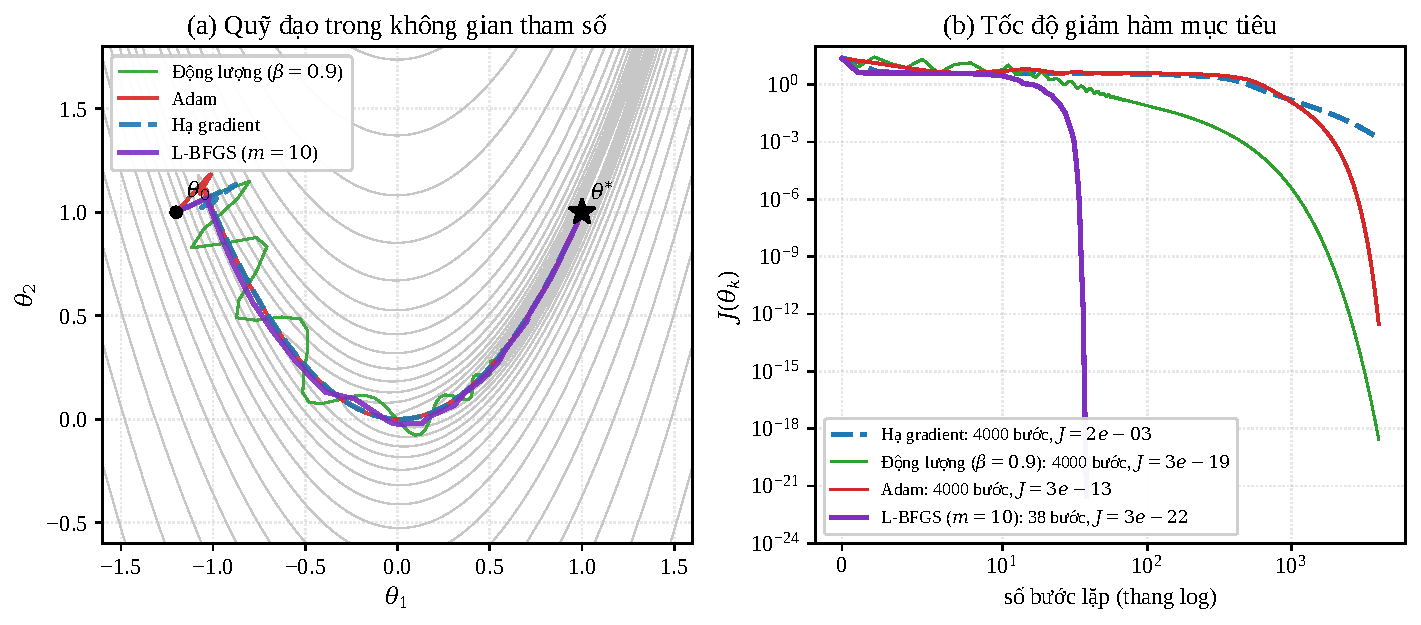
\includegraphics[width=\textwidth]{Images/chap_3/hinh_quydao.pdf}
\caption{So sánh bốn thuật toán tối ưu trên hàm Rosenbrock, cùng điểm xuất phát
$\btheta_0 = (-1{,}2;\,1)$ và cùng nghiệm $\btheta^{\star}=(1;\,1)$. (a) Quỹ đạo
trên nền đường mức; (b) giá trị hàm mục tiêu theo số bước lặp, cả hai trục đều ở
thang lô-ga-rít. Đường L-BFGS dốc đứng ở phía trái phản ánh tốc độ hội tụ siêu
tuyến tính của phương pháp tựa Newton (Nhận xét~\ref{nx:toc-do}).}
\label{fig:quydao}
\end{figure}
 
Cần đọc Hình~\ref{fig:quydao} với một dè dặt: hàm Rosenbrock là hàm hai biến, tất
định, và có nghiệm duy nhất -- không mang ba đặc điểm khó của
Mục~\ref{subsec:dac-thu}. Nó minh hoạ \emph{cơ chế} (thông tin độ cong giúp duỗi
thẳng khe hẹp), không chứng minh điều gì về hàm mục tiêu PINN. Ba lập luận sau
mới là lý do thực chất khiến L-BFGS vượt trội ở giai đoạn cuối trong bối cảnh của
báo cáo.
 
\emph{Thứ nhất, tính tất định.} Trong bài toán PINN, hàm mục tiêu được tính trên
một tập điểm phối trí \emph{cố định}, nên $J(\btheta)$ là hàm tất định và
$\nabla J$ là gradient chính xác chứ không phải ước lượng ngẫu nhiên. Điều kiện
tiên quyết để dùng phương pháp tựa Newton -- các cặp $(\bm{s}_k,\bm{y}_k)$ phản
ánh đúng độ cong -- do đó được thoả mãn. Với gradient nhiễu, hiệu
$\bm{y}_k = \nabla J(\btheta_{k+1}) - \nabla J(\btheta_k)$ là hiệu của hai đại
lượng gần nhau cộng nhiễu, nên phương trình cát tuyến bị bóp méo và xấp xỉ
Hessian nhanh chóng vô nghĩa. Đó là lý do L-BFGS ít được dùng trong học sâu quy
mô lớn với dữ liệu khổng lồ, nhưng lại rất phù hợp ở đây.
 
\emph{Thứ hai, sàn nhiễu.} Theo Mệnh đề~\ref{md:san-nhieu} và
Nhận xét~\ref{nx:noise-floor}, Adam với bước học hằng số chỉ tiệm cận tới một lân
cận của điểm dừng, với mức sàn tỉ lệ tuyến tính theo $\alpha$. Muốn giảm sai số
thêm một bậc, phải giảm bước học một bậc, và tốc độ tiến triển chậm dần tương
ứng. Ngược lại, L-BFGS với tìm kiếm đường Wolfe không có sàn như vậy: nó tiếp tục
giảm $J$ cho tới khi gặp giới hạn của chính số học dấu phẩy động.
 
\emph{Thứ ba, điều kiện xấu.} Hàm mục tiêu \eqref{eq:pinn-loss} là tổng có trọng
của nhiều thành phần có thang độ khác nhau, tạo ra một Hessian có số điều kiện
lớn với các hướng riêng không song song với hệ trục toạ độ. Theo
Nhận xét~\ref{nx:adam-duong-cheo}, xấp xỉ đường chéo của Adam bất lực trước cấu
trúc này, trong khi $\bm{H}_k$ đầy của L-BFGS nắm bắt được tương quan giữa các
toạ độ.
 
Điều ngược lại cũng đúng ở giai đoạn đầu. Khi $\btheta_0$ còn xa nghiệm, mô hình
bậc hai không đáng tin, giả thiết lồi mạnh địa phương của
Nhận xét~\ref{nx:toc-do} không thoả, tìm kiếm đường tốn nhiều lần đánh giá hàm,
và L-BFGS dễ lao thẳng vào cực tiểu địa phương gần nhất -- mà theo
Nhận xét~\ref{nx:doi-xung-hoan-vi}, số lượng cực tiểu như vậy là khổng lồ. Nhiễu
ngẫu nhiên của Adam khi đó lại là một ưu điểm, giúp thoát khỏi các vùng phẳng và
cực tiểu nông.
 
Từ hai nhận định đối lập này, chiến lược chuẩn -- và cũng là chiến lược sẽ áp
dụng ở Chương~\ref{chap:thucnghiem} -- là \emph{huấn luyện hai giai đoạn}.
 
\begin{algorithm}[htbp]
\caption{Chiến lược huấn luyện hai giai đoạn Adam $\to$ L-BFGS}
\label{alg:two-stage}
\begin{algorithmic}[1]
\Require Tham số khởi tạo $\btheta_0$ theo Xavier \eqref{eq:xavier}, số
  vòng $K_{\text{Adam}}$, ngưỡng $\tau$, bộ nhớ $m$
\State \textbf{Giai đoạn 1 (thăm dò).} Chạy Adam
  (Thuật toán~\ref{alg:adam}) với $\alpha = 10^{-3}$ trong $K_{\text{Adam}}$
  vòng lặp, thu $\btheta^{\dagger}$
\State \textbf{Giai đoạn 2 (tinh chỉnh).} Khởi động L-BFGS từ
  $\btheta^{\dagger}$ với tìm kiếm đường Wolfe
  \eqref{eq:wolfe1}--\eqref{eq:wolfe2}, bộ nhớ $m$
\State Dừng khi $\|\nabla J\| < \tau$ hoặc khi tìm kiếm đường thất bại
\State \Return $\btheta^{\star}$
\end{algorithmic}
\end{algorithm}
 
Giai đoạn Adam đưa tham số vào đúng lòng chảo hút của một nghiệm tốt; giai đoạn
L-BFGS khai thác thông tin độ cong để hạ sai số xuống mức mà một bộ giải số
truyền thống có thể so sánh được. Điểm chuyển giao $K_{\text{Adam}}$ là siêu tham
số duy nhất thực sự cần cân nhắc của phác đồ: quá sớm thì L-BFGS chưa ở trong
lòng chảo, quá muộn thì lãng phí vòng lặp ở vùng sàn nhiễu.
 
Hiệu quả của phác đồ được kiểm chứng ở Hình~\ref{fig:hoitu} trên một bài toán
khớp hàm mẫu $u(x)=\sin(3x)\,e^{-x^2/2}$ bằng mạng $(1,16,16,1)$ với hàm kích
hoạt $\tanh$, khởi tạo Xavier, dùng $201$ điểm phân bố đều trên $[-3,3]$. Cài đặt
hoàn toàn bằng NumPy với lan truyền ngược viết tay theo đúng
\eqref{eq:bp1}--\eqref{eq:bp4}, nên hình vẽ phản ánh chính xác lý thuyết đã trình
bày chứ không phải hành vi của một thư viện. Kết quả rõ rệt: Adam chạy đơn thuần
$20\,000$ vòng chững lại ở $J \approx 7{,}7\cdot 10^{-7}$ và dao động quanh mức
đó -- đúng hiện tượng sàn nhiễu của Mệnh đề~\ref{md:san-nhieu} -- trong khi chỉ
cần $2000$ vòng Adam rồi chuyển sang L-BFGS, hàm mục tiêu tiếp tục giảm đều đặn
xuống $J \approx 9{,}1\cdot 10^{-10}$, tốt hơn khoảng $850$ lần với tổng số vòng
lặp tương đương.
 
\begin{figure}[htbp]
\centering
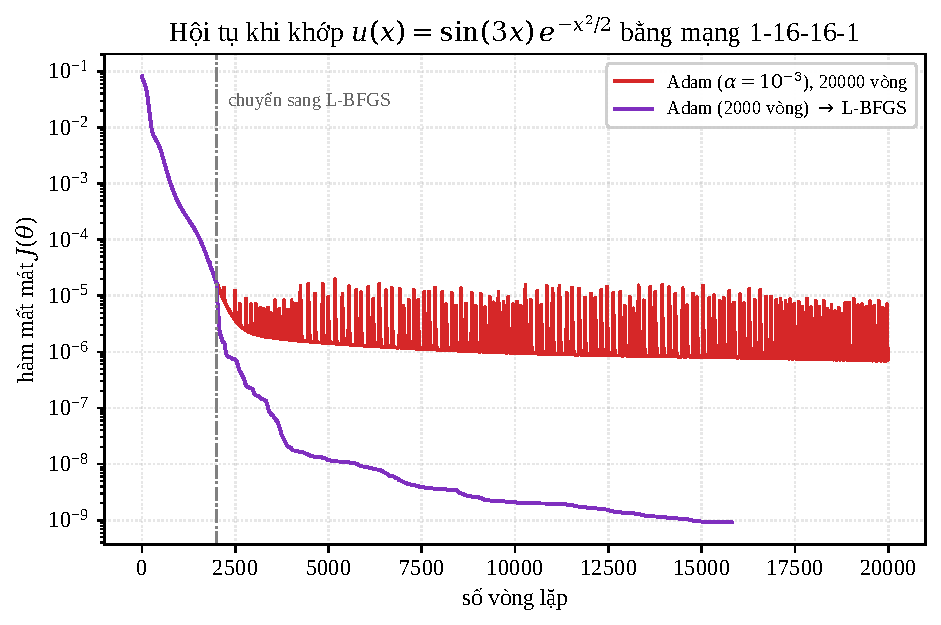
\includegraphics[width=0.86\textwidth]{Images/chap_3/hinh_hoitu.pdf}
\caption{Đường cong hội tụ khi khớp $u(x)=\sin(3x)\,e^{-x^2/2}$ bằng mạng
$(1,16,16,1)$. Đường màu đỏ: Adam với $\alpha=10^{-3}$ chạy liên tục. Đường màu
tím: chiến lược hai giai đoạn, chuyển sang L-BFGS ($m=20$) tại vòng $2000$ (vạch
đứt dọc). Trục tung ở thang lô-ga-rít.}
\label{fig:hoitu}
\end{figure}
 
\begin{nhanxet}[Phạm vi của kết luận]
Thí nghiệm ở Hình~\ref{fig:hoitu} là bài toán \emph{khớp hàm} có nhãn, không phải
bài toán phần dư. Nó kiểm chứng cơ chế sàn nhiễu và lợi ích của giai đoạn tinh
chỉnh trên một hàm mục tiêu tất định, nhưng chưa nói gì về hàm mục tiêu
\eqref{eq:pinn-loss} với nhiều thành phần cạnh tranh. Kết quả định lượng của
chiến lược này trên các bài toán đạo hàm riêng sẽ được trình bày ở
Chương~\ref{chap:thucnghiem}, và cần được đọc như phần kiểm chứng thực sự của
Mục này. Ngoài ra, con số ``$850$ lần'' đến từ một hạt giống ngẫu nhiên; theo
Nhận xét~\ref{nx:doi-xung-hoan-vi}, mọi so sánh giữa hai phác đồ huấn luyện phải
được lặp lại trên nhiều hạt giống trước khi rút kết luận.
\end{nhanxet}
 
%==============================================================================
\section*{Kết luận chương}
\addcontentsline{toc}{section}{Kết luận chương}
%==============================================================================
 
Chương này đã thiết lập bộ công cụ tính toán cho phần còn lại của báo cáo; các
kết quả chính được tổng hợp ở Bảng~\ref{tab:tong-ket-3}.
 
Lan truyền ngược được trình bày như một trường hợp riêng của quy tắc dây chuyền
trên đồ thị tính toán \eqref{eq:chain-graph}, dẫn tới bốn phương trình
\eqref{eq:bp1}--\eqref{eq:bp4} và kết quả then chốt của
Mệnh đề~\ref{md:chi-phi-bp}: chi phí tính gradient chỉ bằng một bội số nhỏ của
chi phí đánh giá hàm, độc lập với số tham số.
 
Vi phân tự động được phân biệt rạch ròi với vi phân ký hiệu và vi phân số.
Mệnh đề~\ref{md:fd-rao-can} chứng minh rằng sai phân hữu hạn bị chặn ở bậc
$\eps^{2/3}$ do xung đột giữa sai số cắt cụt và sai số làm tròn, và
Bảng~\ref{tab:fd-error} xác nhận cả hai nhánh tiệm cận. Quan trọng hơn,
Mệnh đề~\ref{md:ad-tai-tao} khép lại mắt xích còn để ngỏ ở cuối
Chương~\ref{chap:fnn}: cơ chế thuận-trên-thuận của vi phân tự động tái tạo
\emph{đúng} hai hệ thức truy hồi \eqref{eq:G-truy-hoi} và \eqref{eq:S-truy-hoi},
mà không đòi hỏi lập trình tường minh $\sigma''$.
 
Về tối ưu hoá, hai thuật toán đại diện cho hai triết lý đã được phân tích cùng
với chứng minh cho những khẳng định mà tài liệu thường chỉ nêu định tính: sàn
nhiễu của bước học hằng số (Mệnh đề~\ref{md:san-nhieu}), hệ số khuếch đại
$1/(1-\beta)$ của động lượng (Bổ đề~\ref{bd:momentum}), tính cần thiết của hiệu
chỉnh độ chệch trong Adam (Bổ đề~\ref{bd:adam-bias}), và việc điều kiện Wolfe kéo
theo điều kiện độ cong (Bổ đề~\ref{bd:wolfe-curvature}). Chiến lược hai giai đoạn
Adam $\to$ L-BFGS được biện minh bằng ba lập luận -- tính tất định của gradient,
sàn nhiễu, và điều kiện xấu -- chứ không bằng kinh nghiệm thực hành.
 
\begin{table}[htbp]
\centering
\caption{Tổng kết các kết quả chính của Chương~\ref{chap:autodiff}.}
\label{tab:tong-ket-3}
\small
\begin{tabular}{@{}l p{8.2cm}@{}}
\toprule
\textbf{Kết quả} & \textbf{Nội dung và vai trò} \\
\midrule
Mệnh đề~\ref{md:bp}
  & Bốn phương trình lan truyền ngược cho mạng lớp ra tuyến tính; dạng lô
    \eqref{eq:bp-batch}. \\
Mệnh đề~\ref{md:chi-phi-bp}
  & $\mathrm{cost}(\nabla_{\btheta}J) \le 3\,\mathrm{cost}(J)$, độc lập $P$;
    trường hợp riêng có hằng số cụ thể của Định lý~\ref{dl:cheap-gradient}. \\
Mệnh đề~\ref{md:fd-rao-can}
  & Sai phân trung tâm có đáy sai số bậc $\eps^{2/3}$ tại
    $h^{*}\sim\eps^{1/3}$; hằng số phụ thuộc bài toán
    (Nhận xét~\ref{nx:fd-hang-so}). \\
Bổ đề~\ref{bd:doi-ngau}
  & Số đối ngẫu: $f(a+b\epsilon) = f(a)+f'(a)b\epsilon$ -- nguyên lý của chế độ
    thuận. \\
Định lý~\ref{dl:cheap-gradient}
  & Nguyên lý gradient rẻ: hằng số không phụ thuộc số biến. \\
\textbf{Mệnh đề~\ref{md:ad-tai-tao}}
  & \textbf{Vi phân tự động tái tạo đúng các truy hồi
    \eqref{eq:G-truy-hoi}, \eqref{eq:S-truy-hoi} của Chương~\ref{chap:fnn}};
    mỗi lượt cho một dạng toàn phương của Hessian. \\
Mệnh đề~\ref{md:san-nhieu}
  & Sàn nhiễu: $\E[J] \to \alpha\varsigma^2/\big(2(2-\alpha\mu)\big)$, tuyến
    tính theo bước học. \\
Bổ đề~\ref{bd:momentum}
  & Động lượng khuếch đại thành phần nhất quán $1/(1-\beta)$ lần và nén thành
    phần dao động $1/(1+\beta)$ lần. \\
Bổ đề~\ref{bd:adam-bias}
  & $\E[\bm{m}_k] = (1-\beta_1^k)\bm{g}$: hiệu chỉnh độ chệch là cần thiết ở
    các bước đầu. \\
Bổ đề~\ref{bd:wolfe-curvature}
  & Điều kiện Wolfe kéo theo $\bm{y}_k^{\top}\bm{s}_k > 0$, bảo toàn tính xác
    định dương của $\bm{H}_k$. \\
Mệnh đề~\ref{md:two-loop-cost}
  & Đệ quy hai vòng: $\mathcal{O}(mP)$ thời gian và bộ nhớ, không dựng
    $\bm{H}_k$. \\
\bottomrule
\end{tabular}
\end{table}
 
Với nền tảng này, Chương~\ref{chap:pinn} có thể tập trung vào nội dung riêng của
phương pháp: cách xây dựng hàm mục tiêu từ phần dư phương trình vi phân, cách áp
đặt điều kiện đầu và điều kiện biên -- hoặc bằng ràng buộc mềm qua trọng số
$\lambda$ trong \eqref{eq:pinn-loss}, hoặc bằng ràng buộc cứng qua nghiệm thử --
và các đặc tính hội tụ của mạng nơ-ron thông tin vật lý.
 

% Chương 4
\input{Sections/4_}

% Chương 5
\chapter{Triển khai bằng PyTorch và đánh giá số}
\label{chap:thucnghiem}
 
Chương~\ref{chap:pinn} đã thiết lập bằng chứng minh một loạt phát biểu về hành vi
của mạng nơ-ron thông tin vật lý: điều kiện chính quy bắt buộc lên hàm kích hoạt,
chặn ổn định nối phần dư với sai số, cơ chế khuếch đại phổ của toán tử vi phân, và
tính không khả thi của việc học trọng số cân bằng bằng hạ gradient. Mọi phát biểu
ấy đều là những khẳng định \emph{kiểm chứng được}. Chương này thực hiện việc kiểm
chứng đó.
 
Mục tiêu không dừng ở chỗ trình bày một cài đặt chạy được. Mỗi thí nghiệm dưới
đây được thiết kế để trả lời một câu hỏi cụ thể do Chương~\ref{chap:pinn} đặt ra,
với tiêu chí thành công hoặc thất bại xác định \emph{trước} khi chạy. Ta báo cáo
đầy đủ cả những chỗ khớp lẫn những chỗ không khớp: trong chín hạng mục đối chiếu
ở Mục~\ref{sec:doi-chieu}, năm khớp trọn vẹn, một khớp về hướng nhưng không về
độ lớn, một buộc phải siết lại cách phát biểu, một chỉ là tương quan chưa giải
thích được, và một cho kết quả trái với kỳ vọng.
Phần điều chỉnh được ghi rõ thay vì bỏ qua; theo quan điểm của luận văn, một kết
quả tiêu cực được phân tích đúng nguyên nhân có giá trị ngang một kết quả khớp.
 
Cấu trúc chương: Mục~\ref{sec:trienkhai} mô tả kiến trúc cài đặt trên
PyTorch~\cite{paszke2019} và cấu hình chung. Các
Mục~\ref{sec:tn1}--\ref{sec:tn6} trình bày sáu thí nghiệm.
Mục~\ref{sec:doi-chieu} đối chiếu toàn bộ lý thuyết với số liệu, và
Mục~\ref{sec:hanche} nêu thẳng những hạn chế của thiết kế thực nghiệm này.
 
%==============================================================================
\section{Kiến trúc triển khai}
\label{sec:trienkhai}
%==============================================================================
 
\subsection{Đồ thị tính toán động và vi phân tự động lồng nhau}
\label{ssec:ad-pytorch}
 
Đặc điểm khiến PyTorch phù hợp với PINNs là cơ chế \emph{đồ thị tính toán động}
(define-by-run): đồ thị theo Định nghĩa~\ref{def:comp-graph} được dựng lại ở mỗi
lượt xuôi, do đó bản thân \emph{đạo hàm} cũng là một đỉnh trong đồ thị và có thể
tiếp tục vi phân được~\cite{paszke2019}.
 
Theo Mệnh đề~\ref{md:ad-tai-tao}, việc tính $\nabla_{\btheta}r_{\btheta}$ đòi hỏi
vi phân một biểu thức vốn đã chứa $\partial_{\bxi}u_{\btheta}$. Điều kiện kỹ thuật
để thực hiện được là truyền cờ \texttt{create\_graph=True} vào
\texttt{torch.autograd.grad}: cờ này yêu cầu giữ lại đồ thị của phép tính đạo hàm
thay vì giải phóng nó. Nếu thiếu cờ, lời gọi \texttt{backward()} tiếp theo sẽ báo
lỗi hoặc -- nguy hiểm hơn -- trả về gradient bằng không mà không cảnh báo, đúng
tình huống đã nêu ở cuối Mục~\ref{subsec:bac-cao-ad}.
 
\begin{lstlisting}[caption={Toán tử đạo hàm lồng nhau theo biến đầu vào.},label={lst:grad}]
def grad(y, x, order=1):
    """Dao ham cap `order` cua y theo x, giu lai do thi de vi phan tiep."""
    for _ in range(order):
        y = torch.autograd.grad(y, x, torch.ones_like(y),
                                create_graph=True)[0]
    return y
\end{lstlisting}
 
Hàm ở Đoạn mã~\ref{lst:grad} là hiện thực trực tiếp của các công thức truy hồi
\eqref{eq:G-truy-hoi} và \eqref{eq:S-truy-hoi}: mỗi lần lặp trong vòng
\texttt{for} tương ứng với một bậc trong truy hồi Jacobi--Hessian
(Mệnh đề~\ref{md:jacobian} và \ref{md:hessian}), và chi phí nhân lên theo hệ số
hằng đúng như Nhận xét~\ref{nx:chi-phi-bac-cao} dự báo. Cần lưu ý rằng vectơ
$\texttt{torch.ones\_like(y)}$ ở đối số thứ ba chính là vectơ mầm $\bm{w}$ trong
định nghĩa biến liên hợp \eqref{eq:adjoint}: hàm này thực hiện một tích
vectơ--Jacobi \eqref{eq:vjp}, không dựng ma trận Jacobi.
 
\subsection{Mạng nơ-ron và khởi tạo}
 
\begin{lstlisting}[caption={Mạng truyền thẳng với khởi tạo Xavier và nhúng đặc trưng Fourier tuỳ chọn.},label={lst:fnn}]
class FNN(nn.Module):
    def __init__(self, layers, act="tanh", fourier_m=0, fourier_s=1.0):
        super().__init__()
        self.fourier_m = fourier_m
        if fourier_m > 0:                      # nhung dac trung Fourier
            B = torch.randn(fourier_m, layers[0]) * fourier_s
            self.register_buffer("B", B)       # B co dinh, khong hoc
            layers = [2 * fourier_m] + layers[1:]
        self.lins = nn.ModuleList(
            [nn.Linear(layers[i], layers[i+1]) for i in range(len(layers)-1)])
        for lin in self.lins:                  # khoi tao Xavier (Muc 2.3)
            nn.init.xavier_normal_(lin.weight)
            nn.init.zeros_(lin.bias)
        self.act = {"tanh": torch.tanh, "relu": torch.relu}[act]
 
    def forward(self, x):
        if self.fourier_m > 0:
            p = 2 * math.pi * x @ self.B.T
            x = torch.cat([torch.cos(p), torch.sin(p)], dim=1)
        for lin in self.lins[:-1]:
            x = self.act(lin(x))
        return self.lins[-1](x)
\end{lstlisting}
 
Ba lựa chọn trong Đoạn mã~\ref{lst:fnn} tương ứng trực tiếp với ba kết luận của
Chương~\ref{chap:fnn}. Khởi tạo Xavier là \eqref{eq:xavier} với độ chệch bằng
$\bm{0}$, đúng quy ước (A2) của Mục~\ref{subsec:phuong-sai}; ta dùng dạng
\emph{chuẩn tắc} (\texttt{xavier\_normal\_}) chứ không phải dạng đều
\eqref{eq:xavier-uniform}, và theo Nhận xét~\ref{nx:xavier-dang} hai dạng cho
cùng phương sai nên mọi kết quả của Chương~\ref{chap:fnn} áp dụng như nhau. Vòng lặp
\texttt{for lin in self.lins[:-1]} bỏ hàm kích hoạt ở lớp cuối, hiện thực quy ước
lớp ra tuyến tính \eqref{eq:fnn-output}. Ma trận $B$ của nhúng Fourier được đăng
ký bằng \texttt{register\_buffer} chứ không phải \texttt{Parameter}: nó cố định,
không tham gia tối ưu -- một quyết định thiết kế sẽ được kiểm chứng ở
Thí nghiệm~\ref{tn:pho}.
 
Toàn bộ tính toán dùng \texttt{float64}. Lựa chọn này không tuỳ tiện. Ở giai đoạn
L-BFGS, $J_r$ cần đạt tới bậc $10^{-8}$ hoặc nhỏ hơn, trong khi \texttt{float32}
chỉ có khoảng bảy chữ số thập phân có nghĩa. Quan trọng hơn, theo
Nhận xét~\ref{nx:fd-pde}, sai số ở phần dư không bị dập tắt mà được khuếch đại
qua toàn bộ quá trình huấn luyện; độ chính xác kép là điều kiện cần để phân biệt
sai số xấp xỉ với sai số làm tròn, tức để các con số trong chương này có nghĩa.
 
\subsection{Phần dư và quy trình huấn luyện hai giai đoạn}
 
\begin{lstlisting}[caption={Phần dư của phương trình Burgers và vòng huấn luyện.},label={lst:train}]
def residual(net, X):                 # X = (x, t), yeu cau requires_grad_(True)
    u  = net(X)
    g  = grad(u, X)                   # [du/dx, du/dt]
    ut, ux = g[:, 1:2], g[:, 0:1]
    uxx = grad(ux, X)[:, 0:1]         # dao ham bac hai -> can create_graph
    return ut + u * ux - NU * uxx
 
# --- Giai doan 1: Adam ---
opt = torch.optim.Adam(net.parameters(), lr=1e-3)
for it in range(adam_iters + 1):
    Jr = (residual(net, Xr) ** 2).mean()
    Jb = (net(Xb) ** 2).mean()        # hop le vi g == 0 tren bien
    J0 = ((net(X0) - u0) ** 2).mean()
    J  = Jr + lam_b * Jb + lam_0 * J0
    opt.zero_grad(); J.backward(); opt.step()
 
# --- Giai doan 2: L-BFGS voi tim kiem duong Wolfe manh ---
opt2 = torch.optim.LBFGS(net.parameters(), max_iter=800, history_size=50,
                         line_search_fn="strong_wolfe")
opt2.step(closure)
\end{lstlisting}
 
Quy trình hai giai đoạn ở Đoạn mã~\ref{lst:train} hiện thực đúng
Thuật toán~\ref{alg:two-stage}, được lập luận ở Mục~\ref{subsec:adam-vs-lbfgs}
bằng ba lý do: tính tất định của gradient, sàn nhiễu
(Mệnh đề~\ref{md:san-nhieu}), và điều kiện xấu. Tham số
\texttt{line\_search\_fn="strong\_wolfe"} không phải tuỳ chọn: theo
Bổ đề~\ref{bd:wolfe-curvature}, nó là điều kiện để $\bm{H}_k$ giữ tính xác định
dương. Hiệu quả định lượng của bước chuyển được đo ở Mục~\ref{sec:tn4}.
 
Một chi tiết cài đặt đáng nêu: dòng \texttt{Jb = (net(Xb) ** 2).mean()} chỉ đúng
vì mọi bài toán trong chương có điều kiện biên thuần nhất $g \equiv 0$. Với
$g \not\equiv 0$ phải viết \texttt{((net(Xb) - g\_b) ** 2).mean()}. Ta nêu vì đây
là lỗi im lặng: chương trình vẫn chạy và hàm mục tiêu vẫn giảm.
 
\subsection{Công cụ đo: chỉ số mất cân bằng gradient}
\label{ssec:rho}
 
Để đo bệnh lý gradient ở Mục~\ref{sec:gradient-pathology} một cách định lượng, ta
dùng chính đại lượng xuất hiện trong quy tắc \eqref{eq:lambda-hat} của
Thuật toán~\ref{alg:annealing}.
 
\begin{definition}[Chỉ số mất cân bằng gradient]
\label{dn:rho}
Với hàm mục tiêu ở dạng \eqref{eq:loss-compact}, \emph{chỉ số mất cân bằng} của
thành phần thứ $i$ tại tham số $\btheta$ là
\begin{equation}
\rho_i(\btheta)
 := \frac{\norm{\nabla_{\btheta} J_r(\btheta)}_{\infty}}
         {\tfrac{1}{P}\norm{\nabla_{\btheta} J_i(\btheta)}_{1}} .
\label{eq:rho}
\end{equation}
Ta nói bài toán \emph{mắc bệnh lý gradient} đối với thành phần $i$ nếu
$\rho_i \gg 1$ \emph{và} $\rho_i$ tăng theo số vòng lặp huấn luyện.
\end{definition}
 
Điều kiện thứ hai trong Định nghĩa~\ref{dn:rho} là điều kiện thực chất và cần
được nhấn mạnh, vì bài toán khuếch tán ở Mục~\ref{sec:tn4} sẽ cho thấy một
bài toán có
$\rho_b = 25{,}4$ tại khởi tạo nhưng \emph{giảm} sau đó, và việc can thiệp vào bài
toán ấy phản tác dụng. Giá trị tuyệt đối của $\rho_i$ tại một thời điểm không đủ
để chẩn đoán; xu hướng mới đủ.
 
\begin{lstlisting}[caption={Đo chỉ số mất cân bằng $\rho_i$ theo \eqref{eq:rho}.},label={lst:rho}]
def imbalance(loss_r, loss_i, params):
    """rho_i = max|grad J_r| / mean|grad J_i|   (Dinh nghia 5.1)."""
    gr = flat_grad(loss_r, params)     # can retain_graph=True
    gi = flat_grad(loss_i, params)
    return gr.abs().max().item() / gi.abs().mean().item()
\end{lstlisting}
 
Theo Mệnh đề~\ref{md:chi-phi-bp}, mỗi lượt ngược riêng rẽ tốn xấp xỉ chi phí một
lượt xuôi, nên việc đo $\rho_i$ đắt gấp $M+1$ lần một bước huấn luyện thường. Ta
chỉ đo mỗi $100$ vòng lặp.
 
\subsection{Cấu hình thí nghiệm và chỉ tiêu đánh giá}
\label{ssec:cauhinh}
 
\begin{table}[H]
\centering
\caption{Cấu hình chung của các thí nghiệm. Mọi lần chạy dùng hạt giống cố định
để tái lập được; hạn chế của lựa chọn này được nêu ở Mục~\ref{sec:hanche}.}
\label{tab:cauhinh}
\small
\begin{tabular}{@{}p{4.3cm}p{9.2cm}@{}}
\toprule
\textbf{Hạng mục} & \textbf{Thiết lập} \\
\midrule
Thư viện & PyTorch, NumPy; độ chính xác \texttt{float64} \\
Phần cứng & 1 lõi CPU, không dùng GPU \\
Hàm kích hoạt & $\tanh$ (trừ thí nghiệm đối chứng ReLU ở Mục~\ref{sec:tn1}) \\
Khởi tạo & Xavier dạng chuẩn tắc, $\Var(w^{(\ell)}) = 2/(n_{\ell-1}+n_{\ell})$
  theo \eqref{eq:xavier}; $\bb^{(\ell)} = \bm{0}$ \\
Kiến trúc bài toán 1D & $(1,32,32,32,1)$, $2\,209$ tham số \\
Kiến trúc bài toán 2D & $(2,32,32,32,32,1)$, $3\,297$ tham số \\
Kiến trúc bài toán đa tần số & $(1,64,64,64,1)$, $8\,513$ tham số \\
Tối ưu giai đoạn 1 & Adam, $\eta = 10^{-3}$, $\beta = (0{,}9;\,0{,}999)$ \\
Tối ưu giai đoạn 2 & L-BFGS, \texttt{history\_size}${}=50$, Wolfe mạnh \\
Lấy mẫu điểm phối trí & Lưới đều (1D) hoặc lấy mẫu đều ngẫu nhiên (2D) \\
\bottomrule
\end{tabular}
\end{table}
 
Số tham số trong Bảng~\ref{tab:cauhinh} khớp với công thức \eqref{eq:so-tham-so}:
với kiến trúc $(1,32,32,32,1)$ ta có
$P = (1\cdot32+32) + 2\times(32\cdot32+32) + (32\cdot1+1) = 64 + 2112 + 33
= 2\,209$.
 
\begin{definition}[Chỉ tiêu sai số]
\label{dn:chi-tieu}
Gọi $\{\bxi_j\}_{j=1}^{M}$ là lưới đánh giá, \emph{khác} với tập điểm phối trí
huấn luyện, và $u^{\star}$ là nghiệm đúng hoặc nghiệm tham chiếu. Ta dùng
\begin{equation}
\varepsilon_{L^2}
 := \frac{\Big(\sum_{j}\abs{u_{\btheta}(\bxi_j)
      - u^{\star}(\bxi_j)}^2\Big)^{1/2}}
         {\Big(\sum_{j}\abs{u^{\star}(\bxi_j)}^2\Big)^{1/2}},
\qquad
\varepsilon_{L^{\infty}}
 := \max_{j}\abs{u_{\btheta}(\bxi_j) - u^{\star}(\bxi_j)}.
\label{eq:chi-tieu}
\end{equation}
\end{definition}
 
Việc đánh giá trên lưới \emph{khác} tập huấn luyện là bắt buộc chứ không phải cẩn
trọng thừa. Nhận xét~\ref{rem:monte-carlo} đã lập luận rằng $J_r$ mất tính không
chệch ngay khi $\btheta$ được tối ưu trên chính tập mẫu sinh ra nó: giá trị $J_r$
cuối cùng là ước lượng chệch xuống của $\norm{r_{\btheta}}^2_{L^2}$. Sai số đo
trên lưới độc lập mới phản ánh chất lượng nội suy thực sự.
 
%==============================================================================
\section{Thí nghiệm 1: hàm kích hoạt và sự suy biến của ReLU}
\label{sec:tn1}
%==============================================================================
 
\begin{thinghiem}[Kiểm chứng Hệ quả~\ref{hq:pinn-hong}]
\label{tn:relu}
Hệ quả~\ref{hq:pinn-hong} khẳng định mạng ReLU cho
$\partial_{xx}u_{\btheta} = 0$ hầu khắp nơi
(Hệ quả~\ref{hq:relu-hkn}), dẫn tới $J_r$ hằng địa phương với giá trị
$\overline{f^2}$ và $\nabla_{\btheta}J_r \equiv \bm{0}$. Đây là khẳng định về
\emph{đẳng thức chính xác}, không phải về ``hội tụ chậm'', nên có thể kiểm chứng
tới từng chữ số máy.
\end{thinghiem}
 
\textbf{Thiết lập.} Bài toán Poisson một chiều với nghiệm chế tạo:
\begin{equation}
-u''(x) = f(x) \ \text{ trên } (0,1),
\qquad u(0) = u(1) = 0,
\qquad u^{\star}(x) = \sin(2\pi x),
\label{eq:poisson-tn1}
\end{equation}
do đó $f(x) = 4\pi^2\sin(2\pi x)$. Đây chính là bài toán của
Mệnh đề~\ref{md:chan-on-dinh}, nên ta có sẵn chặn ổn định
$\norm{e_{\btheta}}_{L^2} \le \pi^{-2}\norm{r_{\btheta}}_{L^2}$ để đối chiếu.
Huấn luyện $4\,000$ vòng Adam với $256$ điểm phối trí đều, $\lambda_b = 100$, hai
hàm kích hoạt $\tanh$ và ReLU trên cùng kiến trúc và cùng hạt giống.
 
\begin{table}[H]
\centering
\caption{So sánh hai hàm kích hoạt trên bài toán Poisson \eqref{eq:poisson-tn1}.}
\label{tab:tn1}
\small
\begin{tabular}{@{}lrrrr@{}}
\toprule
\textbf{Hàm kích hoạt} & $\varepsilon_{L^2}$ & $\varepsilon_{L^{\infty}}$
& $J_r$ cuối & $\norm{\nabla_{\btheta}J_r}_{\infty}$ \\
\midrule
$\tanh$ & $5{,}977\times10^{-5}$ & $8{,}701\times10^{-5}$
        & $2{,}463\times10^{-3}$ & --- \\
ReLU    & $9{,}991\times10^{-1}$ & $1{,}004\times10^{0}$
        & $7{,}762\times10^{2}$  & $0{,}0$ \\
\bottomrule
\end{tabular}
\end{table}
 
\textbf{Kết quả.} Ba con số dưới đây là bằng chứng trực tiếp cho từng khẳng định
của Hệ quả~\ref{hq:pinn-hong}.
 
\begin{enumerate}[label=(\alph*),leftmargin=2.2em,itemsep=3pt]
\item \emph{Đạo hàm bậc hai triệt tiêu.} Đo trực tiếp trên mạng ReLU tại khởi tạo
cho $\max_{x}\abs{\partial_{xx}u_{\btheta}(x)} = 0{,}0$ \emph{chính xác} -- không
phải một số nhỏ -- vì \texttt{autograd} truyền $\sigma'' \equiv 0$ qua toàn bộ đồ
thị, đúng theo truy hồi \eqref{eq:ad-hvp}: số hạng thứ nhất triệt tiêu ở mọi lớp,
số hạng thứ hai không có gì để truyền.
 
\item \emph{Hàm mục tiêu hằng.} Giá trị đo được $J_r = 776{,}229$. Đối chiếu:
giá trị liên tục là
$\overline{f^2} = \int_0^1 16\pi^4\sin^2(2\pi x)\,dx = 8\pi^4 = 779{,}273$, còn
trung bình của $f^2$ \emph{trên đúng lưới đánh giá $1\,001$ điểm} là
$778{,}494$. Sai lệch giữa $776{,}229$ và $778{,}494$ là $0{,}29\%$, do hai lưới
cầu phương khác nhau ($256$ điểm huấn luyện so với $1\,001$ điểm đánh giá) chứ
không do mạng. Ta nêu cả hai giá trị tham chiếu vì việc chỉ nêu một trong hai dễ
gây hiểu nhầm về nguồn sai lệch.
 
\item \emph{Gradient triệt tiêu.} $\norm{\nabla_{\btheta}J_r}_{\infty} = 0{,}0$
và $\norm{\nabla_{\btheta}J_r}_{2} = 0{,}0$, đúng bằng không trong số học dấu
phẩy động -- không phải nhỏ dưới một ngưỡng.
\end{enumerate}
 
Sai số $\varepsilon_{L^2} = 0{,}9991 \approx 1$ của mạng ReLU có nghĩa hình học
rõ ràng: mạng hội tụ về $u_{\btheta} \approx 0$. Nó chỉ học được điều kiện biên --
thành phần duy nhất còn gradient -- và hoàn toàn mù trước phương trình. Chênh lệch
độ chính xác giữa hai hàm kích hoạt là $1{,}67\times 10^{4}$ lần.
 
\begin{figure}[H]
\centering
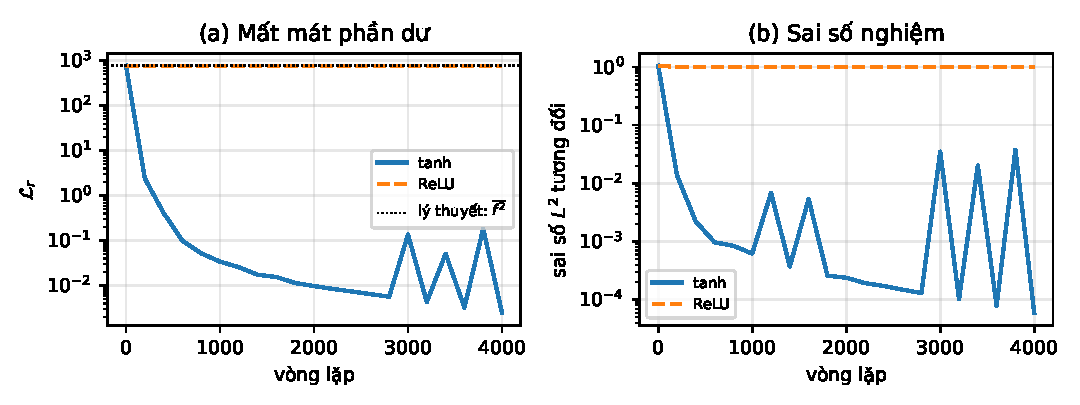
\includegraphics[width=\textwidth]{Images/chap_5/fig51_relu.pdf}
\caption{Bài toán Poisson \eqref{eq:poisson-tn1} với hai hàm kích hoạt. (a) Mất
mát phần dư của mạng ReLU nằm đúng trên đường lý thuyết $\overline{f^2}$ và không
hề giảm suốt $4\,000$ vòng lặp. (b) Sai số $L^2$ tương ứng.}
\label{fig:tn1}
\end{figure}
 
\begin{nhanxet}[Dấu hiệu chẩn đoán]
Hình~\ref{fig:tn1}(a) cho một quy tắc thực dụng: nếu $J_r$ của một PINN nằm phẳng
tuyệt đối \emph{ngay từ vòng lặp đầu tiên}, nguyên nhân gần như chắc chắn là bậc
khả vi của hàm kích hoạt thấp hơn bậc của toán tử vi phân, chứ không phải tốc độ
học hay khởi tạo. Dấu hiệu phân biệt là chữ ``ngay từ đầu'': một bài toán khó
nhưng đúng kiến trúc vẫn giảm $J_r$ ở những vòng đầu rồi mới chững lại theo cơ chế
sàn nhiễu (Mệnh đề~\ref{md:san-nhieu}).
\end{nhanxet}
 
%==============================================================================
\section{Thí nghiệm 2: cái giá của ràng buộc mềm}
\label{sec:tn2}
%==============================================================================
 
Nhận xét~\ref{rem:soft-constraint} đã nêu rằng ràng buộc mềm không được thoả
chính xác, nhưng chưa lượng hoá mức vi phạm. Mệnh đề sau lấp chỗ trống đó; nó là
dạng chuyên biệt hoá của kết quả cổ điển về phương pháp phạt toàn
phương~\cite{nocedal2006}.
 
\begin{menhde}[Sai số biên của phương pháp phạt]
\label{md:phat-bien-phat}
Xét $J_{\lambda}(\btheta) = J_r(\btheta) + \lambda\, c(\btheta)^2$ với
$J_r, c \in C^1$, và giả sử $\btheta_{\lambda}$ là một điểm dừng của
$J_{\lambda}$. Nếu tồn tại các hằng số $0 < a \le A$ và $G$ sao cho
$a \le \norm{\nabla c(\btheta_{\lambda})} \le A$ và
$\norm{\nabla J_r(\btheta_{\lambda})} \le G$ với mọi $\lambda$ đủ lớn, thì
\begin{equation}
\abs{c(\btheta_{\lambda})} \;\le\; \frac{G}{2a}\cdot\frac{1}{\lambda}
 \;=\; \mathcal{O}\!\left(\lambda^{-1}\right).
\label{eq:phat-bac-nhat}
\end{equation}
\end{menhde}
 
\begin{proof}
Điều kiện dừng $\nabla J_{\lambda}(\btheta_{\lambda}) = \bm{0}$ cho
\[
\nabla J_r(\btheta_{\lambda})
 + 2\lambda\, c(\btheta_{\lambda})\,\nabla c(\btheta_{\lambda}) = \bm{0}
\quad\Longrightarrow\quad
2\lambda\,\abs{c(\btheta_{\lambda})}\,\norm{\nabla c(\btheta_{\lambda})}
 = \norm{\nabla J_r(\btheta_{\lambda})} .
\]
Thay chặn dưới $\norm{\nabla c} \ge a$ và chặn trên
$\norm{\nabla J_r} \le G$, rồi chia hai vế cho $2\lambda a$.
\end{proof}
 
Hai giả thiết của Mệnh đề~\ref{md:phat-bien-phat} đáng chú ý. Giả thiết
$\norm{\nabla c} \ge a > 0$ là điều kiện chính quy của ràng buộc; nếu nó hỏng,
quan hệ $\lambda^{-1}$ hỏng theo. Giả thiết $\norm{\nabla J_r} \le G$ nói rằng
gradient phần dư không bùng nổ khi $\lambda$ tăng -- một giả thiết mà chính thí
nghiệm dưới đây sẽ cho thấy bị vi phạm ở đầu $\lambda_b$ lớn.
 
\begin{thinghiem}[Kiểm chứng Mệnh đề~\ref{md:phat-bien-phat}]
\label{tn:lambda}
Quy luật $\lambda_b^{-1}$ được chứng minh cho một điểm dừng chính xác của một mô
hình một ràng buộc. Câu hỏi: nó có sống sót trên bài toán phi tuyến thật, với
$2\,209$ tham số và tối ưu chưa hội tụ hoàn toàn hay không?
\end{thinghiem}
 
\textbf{Thiết lập.} Vẫn bài toán \eqref{eq:poisson-tn1}, cố định
$\lambda_r = 1$ và quét $\lambda_b$ qua sáu bậc độ lớn. Đại lượng đo là
$\max\{\abs{u_{\btheta}(0)}, \abs{u_{\btheta}(1)}\}$.
 
\begin{table}[H]
\centering
\caption{Ảnh hưởng của trọng số biên $\lambda_b$ (bài toán Poisson, $4\,000$ vòng
Adam). Giá trị tốt nhất của mỗi cột được in đậm.}
\label{tab:tn2}
\small
\begin{tabular}{@{}rrrrr@{}}
\toprule
$\lambda_b$ & sai số biên & $\varepsilon_{L^2}$ & $\varepsilon_{L^{\infty}}$
& $J_r$ \\
\midrule
$0{,}01$ & $9{,}117\times10^{-1}$ & $7{,}455\times10^{-1}$
         & $9{,}117\times10^{-1}$ & $2{,}933\times10^{-3}$ \\
$0{,}1$  & $1{,}743\times10^{-2}$ & $1{,}422\times10^{-2}$
         & $1{,}743\times10^{-2}$ & $2{,}415\times10^{-3}$ \\
$1$      & $8{,}033\times10^{-4}$ & $5{,}488\times10^{-4}$
         & $8{,}033\times10^{-4}$ & $2{,}171\times10^{-4}$ \\
$10$     & $1{,}858\times10^{-4}$ & $1{,}437\times10^{-4}$
         & $2{,}053\times10^{-4}$ & $9{,}301\times10^{-4}$ \\
$100$    & $2{,}697\times10^{-5}$ & $\mathbf{5{,}977\times10^{-5}}$
         & $8{,}701\times10^{-5}$ & $2{,}463\times10^{-3}$ \\
$1\,000$ & $\mathbf{1{,}180\times10^{-5}}$ & $3{,}300\times10^{-4}$
         & $3{,}313\times10^{-4}$ & $1{,}028\times10^{-2}$ \\
\bottomrule
\end{tabular}
\end{table}
 
\textbf{Kết quả.} Hồi quy tuyến tính trên thang log--log trong dải
$\lambda_b \in [0{,}1;\,100]$ cho
\begin{equation}
\text{sai số biên} \;\propto\; \lambda_b^{-0{,}907},
\label{eq:do-doc-do}
\end{equation}
so với số mũ $-1$ của Mệnh đề~\ref{md:phat-bien-phat}. Sai lệch $9\%$ ở số mũ là
mức phù hợp tốt, xét rằng mệnh đề được chứng minh tại một \emph{điểm dừng chính
xác} của mô hình một ràng buộc, còn thực nghiệm chạy trên mạng phi tuyến
$2\,209$ tham số sau $4\,000$ vòng Adam -- tức tại một điểm mà theo
Mệnh đề~\ref{md:san-nhieu}, gradient chưa triệt tiêu mà chỉ dao động quanh sàn
nhiễu.
 
Ở đầu $\lambda_b = 0{,}01$, sai số biên bão hoà ở mức $0{,}91$: đúng kịch bản
Nhận xét~\ref{rem:ill-posedness} mô tả. Nghiệm thu được thoả phương trình khá tốt
-- $J_r$ thậm chí nhỏ nhất trong bảng -- nhưng sai hoàn toàn ở biên, tức mạng đã
trôi trên tập $\mathcal{M}_r$ của \eqref{eq:manifold-r} và hội tụ về \emph{một
nghiệm khác} của cùng phương trình vi phân. Đây cũng là minh hoạ cụ thể cho việc
vì sao Mệnh đề~\ref{md:chan-on-dinh} phải giả thiết điều kiện biên thoả chính
xác: ở dòng này, phần dư nhỏ mà sai số lớn.
 
\begin{figure}[H]
\centering
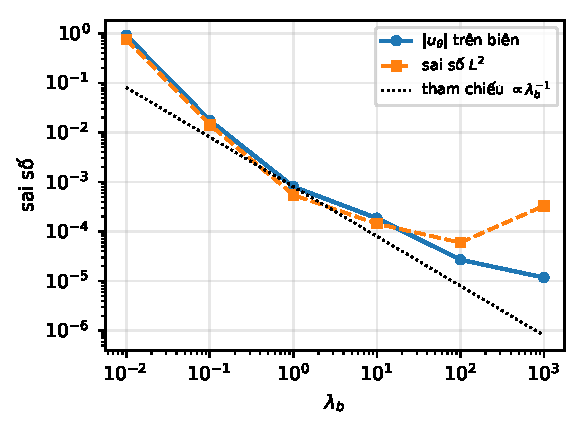
\includegraphics[width=0.55\textwidth]{Images/chap_5/fig52_lambda.pdf}
\caption{Sai số biên và sai số $L^2$ theo $\lambda_b$. Đường chấm là tham chiếu
$\propto \lambda_b^{-1}$ của Mệnh đề~\ref{md:phat-bien-phat}.}
\label{fig:tn2}
\end{figure}
 
\begin{nhanxet}[Đánh đổi mà Mệnh đề~\ref{md:phat-bien-phat} không nắm bắt]
\label{nx:danh-doi}
Cột $\varepsilon_{L^2}$ của Bảng~\ref{tab:tn2} bộc lộ một hiện tượng nằm ngoài
phạm vi mệnh đề. Khi $\lambda_b$ tăng từ $100$ lên $1\,000$, sai số biên tiếp tục
giảm ($2{,}70\times10^{-5} \to 1{,}18\times10^{-5}$) đúng như dự báo, nhưng sai số
$L^2$ \emph{toàn cục lại xấu đi} $5{,}5$ lần
($5{,}98\times10^{-5} \to 3{,}30\times10^{-4}$), đồng thời $J_r$ tăng $4{,}2$
lần.
 
Lý do là Mệnh đề~\ref{md:phat-bien-phat} chỉ theo dõi \emph{một} trong hai mục
tiêu cạnh tranh, và giả thiết $\norm{\nabla J_r} \le G$ của nó bị vi phạm: cột
$J_r$ cho thấy phần dư tăng đơn điệu từ $\lambda_b = 1$ trở đi. Khi $\lambda_b$
quá lớn, điểm tối ưu bị đẩy về đầu kia của đường đánh đổi: điều kiện biên gần như
chính xác, nhưng phần dư trong miền bị hy sinh.
 
Kết luận thực hành: $\lambda_b$ tối ưu theo nghĩa sai số toàn cục là một giá trị
\emph{hữu hạn} -- ở đây $\lambda_b \approx 100$ -- chứ không phải càng lớn càng
tốt. Đây là bổ sung của thực nghiệm cho phân tích lý thuyết ở
Mục~\ref{sec:gradient-pathology}, và nó sẽ tái xuất ở
Mục~\ref{sec:tn4}--\ref{sec:tn5} dưới dạng nguyên nhân khiến thuật toán ủ trọng
số phản tác dụng.
\end{nhanxet}
 
%==============================================================================
\section{Thí nghiệm 3: thiên kiến phổ và sự đảo chiều do toán tử vi phân}
\label{sec:tn3}
%==============================================================================
 
Đây là thí nghiệm quan trọng nhất của chương, vì nó buộc phải siết lại một kết
luận của Chương~\ref{chap:pinn}.
 
\paragraph{Giả thuyết làm việc.}
Chương~\ref{chap:pinn} cho hai thừa số tác động lên tốc độ học của một mode tần
số $\bk$, nhưng chưa ghép chúng thành một công thức. Một mặt,
Nhận xét~\ref{rem:ntk-view} cho tốc độ phân rã của mode thứ $j$ trong bài toán
hồi quy là trị riêng $\varkappa_j$ của nhân tiếp tuyến; viết
$\widehat{\varkappa}(\bk)$ cho ký hiệu phổ của nhân. Mặt khác,
Mệnh đề~\ref{md:khuech-dai} cho biết hàm mục tiêu phần dư nhìn thấy sai số qua ký
hiệu chính $P(\bk)$ của toán tử, với biên độ bị nhân lên $\abs{P(\bk)}$. Vì hàm mục tiêu là bình phương, ta \emph{giả thuyết} rằng tốc độ hiệu dụng là
\begin{equation}
\mu(\bk) \;=\; \abs{P(\bk)}^{2}\,\widehat{\varkappa}(\bk).
\label{eq:pho-hieu-dung}
\end{equation}
Cần nói thẳng: \eqref{eq:pho-hieu-dung} \emph{không} phải một mệnh đề đã chứng
minh trong luận văn. Nó là giả thuyết làm việc ghép từ hai kết quả nói trên, và
mục đích của thí nghiệm này là kiểm tra dự báo định tính của nó.
 
Dự báo ấy như sau. Với toán tử Poisson trong $\R^1$, $P(k) = 4\pi^2k^2$, nên
$\abs{P(k)}^{2} \propto k^{4}$. Nếu $\widehat{\varkappa}(k)$ suy giảm chậm hơn
$k^{-4}$ thì $\mu(k)$ \emph{tăng} theo $k$: hàm mục tiêu phần dư sẽ \emph{ưu tiên
tần số cao} -- ngược hẳn với thiên kiến phổ cổ điển của
Định lý~\ref{dl:spectral-decay}.
 
\begin{thinghiem}[Kiểm tra giả thuyết \eqref{eq:pho-hieu-dung}]
\label{tn:pho}
Đo thứ tự học các mode tần số trên cùng một nghiệm đích, dưới hai hàm mục tiêu
khác nhau: hồi quy ($P \equiv 1$) và phần dư ($P(k) = 4\pi^2k^2$). Nếu
\eqref{eq:pho-hieu-dung} đúng về hướng, hai chế độ phải cho thứ tự học
\emph{ngược nhau}.
\end{thinghiem}
 
\textbf{Thiết lập.} Nghiệm chế tạo đa tần số với biên độ bằng nhau trên $(0,1)$:
\begin{equation}
u^{\star}(x) = \sum_{k \in \{1,4,8\}} \sin(2\pi k x),
\qquad
f(x) = \sum_{k \in \{1,4,8\}} 4\pi^2 k^2 \sin(2\pi k x).
\label{eq:da-tan-so}
\end{equation}
Biên độ bằng nhau là điều kiện thiết kế then chốt: nó bảo đảm mọi khác biệt về
thứ tự học đến từ hàm mục tiêu chứ không từ trọng số ban đầu của các mode. Ba chế
độ huấn luyện trên \emph{cùng} mục tiêu, cùng kiến trúc, cùng hạt giống:
 
\begin{enumerate}[label=(\alph*),leftmargin=2.2em,itemsep=2pt]
\item \textbf{Hồi quy}: $J = \overline{\abs{u_{\btheta} - u^{\star}}^2}$, tức
$P \equiv 1$ và $\mu(k) = \widehat{\varkappa}(k)$. Đây là nhóm đối chứng, đo
thiên kiến phổ \emph{thuần tuý của mạng}.
\item \textbf{Phần dư}: $J = \overline{\abs{-u_{\btheta}'' - f}^2} + 100\,J_b$,
tức $\mu(k) = \abs{P(k)}^2\widehat{\varkappa}(k)$ theo
\eqref{eq:pho-hieu-dung}.
\item \textbf{Phần dư kèm đặc trưng Fourier}: như (b) nhưng thêm nhúng của
Bảng~\ref{tab:remedies} với $M = 32$, $s = 6$.
\end{enumerate}
 
Đại lượng theo dõi là hệ số sai số theo từng mode,
\begin{equation}
c_k(n) = 2\int_0^1 \big(u_{\btheta_n} - u^{\star}\big)\sin(2\pi k x)\,dx,
\label{eq:he-so-mode}
\end{equation}
hợp lệ vì $\int_0^1\sin^2(2\pi kx)\,dx = \tfrac12$, cùng
$t_{10}(k) :=$ số vòng lặp đầu tiên để $\abs{c_k}$ giảm còn $10\%$ giá trị ban
đầu.
 
\begin{table}[H]
\centering
\caption[Thứ tự học các mode tần số]{Thứ tự học các mode tần số. Dấu ``---''
nghĩa là không đạt ngưỡng trong $8\,000$ vòng lặp. \textbf{Cảnh báo khi đọc:}
$t_{10}$ là thời điểm $\abs{c_k}$ chạm ngưỡng $10\%$ \emph{lần đầu}, và đại
lượng này \emph{không đơn điệu} -- một mode có thể đạt ngưỡng rồi bị đẩy ra xa
trở lại. Ở chế độ (b), mode $k=1$ chạm ngưỡng tại vòng $200$ nhưng sau đó phân
kỳ tới $\abs{c_1} = 6{,}605$ tại vòng $40\,000$ theo \eqref{eq:c-plateau}. Vì
vậy cột $t_{10}$ \emph{không} phản ánh thứ tự học của chế độ (b); căn cứ đúng là
\eqref{eq:c-plateau}.}
\label{tab:tn3}
\small
\begin{tabular}{@{}lrrrr@{}}
\toprule
\textbf{Chế độ} & $t_{10}(k{=}1)$ & $t_{10}(k{=}4)$ & $t_{10}(k{=}8)$
& $\varepsilon_{L^2}$ \\
\midrule
(a) Hồi quy trực tiếp   & $700$    & $1\,100$ & $2\,100$
                        & $7{,}105\times10^{-3}$ \\
(b) Mất mát phần dư     & $200$    & ---      & ---
                        & $5{,}465\times10^{0}$ \\
(c) Phần dư + Fourier   & $4\,200$ & $100$    & $100$
                        & $3{,}393\times10^{-2}$ \\
\bottomrule
\end{tabular}
\end{table}
 
\begin{figure}[H]
\centering
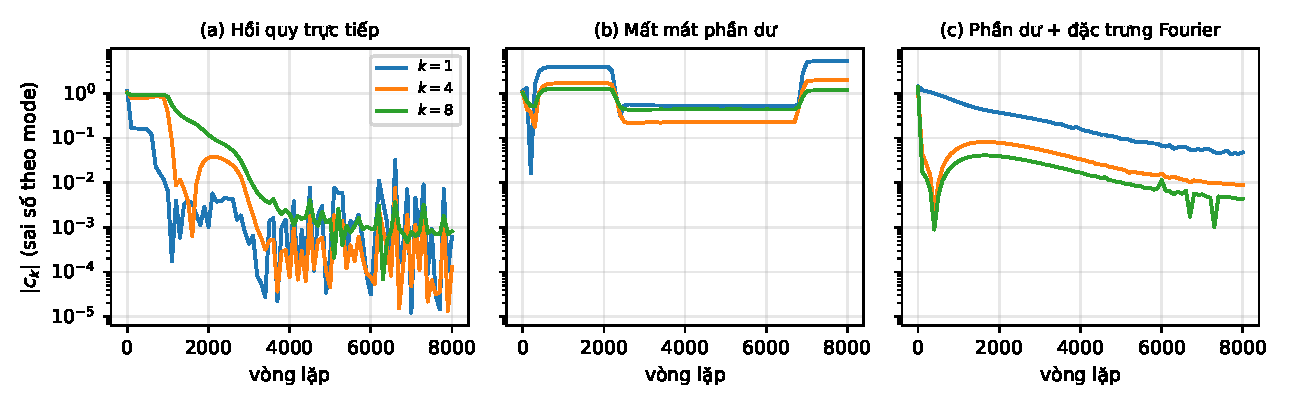
\includegraphics[width=\textwidth]{Images/chap_5/fig53_spectral.pdf}
\caption{Sai số theo từng mode tần số $\abs{c_k}$ trong ba chế độ huấn luyện trên
cùng nghiệm đích \eqref{eq:da-tan-so}.}
\label{fig:tn3}
\end{figure}
 
\textbf{Kết quả và phân tích.}
 
\emph{(a) Thiên kiến phổ cổ điển được xác nhận.} Chế độ hồi quy cho thứ tự học
đơn điệu theo tần số: $700 < 1\,100 < 2\,100$ vòng lặp cho $k = 1, 4, 8$, với tỉ
lệ $t_{10}(8)/t_{10}(1) = 3{,}0$. Đây đúng là nội dung của
Nhận xét~\ref{rem:ntk-view} với $\widehat{\varkappa}$ suy giảm theo tần số, và là
biểu hiện động lực học của Hệ quả~\ref{hq:parameter-cost}.
 
\emph{(b) Toán tử vi phân đảo ngược thứ tự ưu tiên.} Chế độ phần dư thất bại:
$\varepsilon_{L^2} = 5{,}465$, tức sai số lớn hơn cả biên độ nghiệm. Điều đáng nói
là \emph{cấu trúc} của sai số. Một lần chạy đối chứng kéo dài tới $40\,000$ vòng
cho thấy quá trình dừng hẳn từ vòng $20\,000$ (giá trị $\varepsilon_{L^2}$ tại các
mốc $20\,000$, $30\,000$, $40\,000$ lần lượt là $5{,}474$, $5{,}475$, $5{,}475$),
và phân tích theo mode tại vòng $40\,000$ cho
\begin{equation}
\abs{c_1} = 6{,}605,
\qquad
\abs{c_4} = 0{,}821,
\qquad
\abs{c_8} = 0{,}171 .
\label{eq:c-plateau}
\end{equation}
Trong ba mode được theo dõi, sai số tập trung ở mode \emph{tần số thấp nhất}, còn
mode tần số cao nhất được học tốt nhất, với tỉ lệ
$\abs{c_1}/\abs{c_8} = 38{,}6$. Đây đúng là hướng mà \eqref{eq:pho-hieu-dung} dự
báo.

Kết luận này \emph{mâu thuẫn bề ngoài} với cột $t_{10}$ của
Bảng~\ref{tab:tn3}, nơi chế độ (b) cho $t_{10}(k{=}1) = 200$ -- nhanh nhất trong
ba mode -- còn $k = 4$ và $k = 8$ không đạt ngưỡng. Cần giải thích rõ chỗ này vì
nó dễ dẫn tới kết luận ngược. Hai cột đo hai thứ khác nhau: $t_{10}$ là thời
điểm \emph{chạm ngưỡng lần đầu}, còn \eqref{eq:c-plateau} là sai số \emph{tại
điểm dừng}. Với hàm mục tiêu phần dư, quỹ đạo của $\abs{c_1}$ không đơn điệu --
nó giảm qua ngưỡng $10\%$ ở vòng $200$ rồi \emph{bị đẩy ngược trở ra} và ổn định
ở $6{,}605$, tức lớn gấp hơn sáu lần biên độ ban đầu của chính mode đó. Trong
khi ấy $\abs{c_4} = 0{,}821$ và $\abs{c_8} = 0{,}171$ tuy chưa bao giờ chạm
ngưỡng $10\%$ nhưng dừng ở mức thấp hơn hẳn. Vì mục tiêu của thí nghiệm là so
sánh thứ tự \emph{ưu tiên} chứ không phải tốc độ chạm một ngưỡng tuỳ chọn, căn
cứ đúng là \eqref{eq:c-plateau}; cột $t_{10}$ chỉ đọc được như một chỉ báo thứ
tự ở chế độ (a) và (c), nơi nó nhất quán với sai số cuối cùng.
 
Về độ lớn, cần tách hai con số thường bị lẫn. Thừa số $\abs{P(k)}^2 \propto k^4$
\emph{một mình} ưu tiên mode $k=8$ hơn mode $k=1$ một hệ số $8^4 = 4\,096$. Nhưng
$\mu(k)$ trong \eqref{eq:pho-hieu-dung} còn chứa $\widehat{\varkappa}(k)$, vốn suy
giảm theo $k$; với ước lượng thô $\widehat{\varkappa}(k)\sim k^{-2}$ ta được
$\mu(k) \sim k^{2}$ và hệ số ưu tiên chỉ còn $8^2 = 64$. Tỉ lệ đo được $38{,}6$
nằm gần con số thứ hai hơn -- nhưng ta không rút kết luận định lượng từ đối chiếu
này, vì $\abs{c_k}$ tại điểm dừng không phải một hàm đơn giản của $\mu(k)$, và vì
ước lượng $\widehat{\varkappa}(k)\sim k^{-2}$ chưa được chứng minh ở đâu trong
luận văn.
 
\begin{nhanxet}[Ba mode được theo dõi không chiếm hết sai số]
\label{nx:nang-luong}
Một đối chiếu nhất quán nội tại đáng làm. Vì
$\norm{u^{\star}}^2_{L^2(0,1)} = 3/2$, sai số tương đối $5{,}465$ tương ứng
$\norm{e_{\btheta}}^2_{L^2} = 5{,}465^2\times 1{,}5 = 44{,}80$. Trong khi đó ba
mode ở \eqref{eq:c-plateau} chỉ đóng góp
$\tfrac12(6{,}605^2 + 0{,}821^2 + 0{,}171^2) = 22{,}16$, tức $49{,}5\%$ tổng năng
lượng sai số.
 
Vậy khoảng một nửa sai số nằm ở các thành phần \emph{ngoài} ba mode được theo dõi
-- nhiều khả năng là thành phần hằng và các mode tần số thấp khác, những thành
phần mà toán tử $-\partial_{xx}$ nhìn thấy yếu nhất (với hằng số thì
$P(0) = 0$ và toán tử hoàn toàn mù). Điều này củng cố thêm kết luận định tính,
nhưng nó cũng có nghĩa là phát biểu ``toàn bộ sai số nằm ở mode tần số thấp nhất''
sẽ là quá mạnh; phát biểu đúng là ``trong ba mode được theo dõi, sai số tập trung
ở mode thấp nhất''.
\end{nhanxet}
 
Hiện tượng dừng hẳn ở vòng $20\,000$ cũng nhất quán với
Mệnh đề~\ref{md:san-nhieu}: khi độ trải phổ hiệu dụng $\kappa_{\mathrm{eff}}$ lớn,
hướng tần số thấp gần như phẳng ($\mu$ nhỏ), nên bước cập nhật theo hướng đó bị
sàn nhiễu lấn át và không tiến thêm được.
 
\emph{(c) Nhúng Fourier khôi phục khả năng học.} Sai số $L^2$ giảm từ $5{,}465$
xuống $3{,}393\times10^{-2}$, tức cải thiện $161$ lần. Cột $t_{10}$ giải thích cơ
chế: với $s = 6$, dải thông của nhúng đặt trọng tâm ở tần số cao, nên $k = 4$ và
$k = 8$ được học chỉ sau $100$ vòng, còn $k = 1$ trở thành mode chậm nhất
($4\,200$ vòng). Nhúng Fourier không \emph{xoá bỏ} thiên kiến phổ mà \emph{dịch
chuyển} nó, đúng như Bảng~\ref{tab:remedies} đã phân loại. Hệ quả thực hành: tham
số $s$ phải được chọn theo dải tần số của nghiệm cần tìm, và chọn $s$ quá lớn sẽ
đánh mất tần số thấp -- một đòi hỏi khó chịu, vì nó giả thiết ta đã biết trước
thang độ dài của nghiệm chưa biết.
 
\begin{nhanxet}[Siết lại kết luận của Mục~\ref{subsec:he-qua-pinn}]
\label{nx:hieu-chinh}
Mục~\ref{subsec:he-qua-pinn} kết luận rằng ``bài toán đòi hỏi độ chính xác cao
nhất ở đúng những tần số mà mô hình học chậm nhất''.
Thí nghiệm~\ref{tn:pho} cho thấy phát biểu này \emph{không đúng phổ quát}: với
toán tử elliptic thuần tuý, hàm mục tiêu phần dư ưu tiên tần số cao và chính tần
số thấp mới bị bỏ rơi.
 
Không có mâu thuẫn logic giữa hai kết quả, vì \eqref{eq:pho-hieu-dung} có
\emph{hai} thừa số cạnh tranh và dấu của xu hướng phụ thuộc thừa số nào thắng.
Chương~\ref{chap:pinn} chỉ lập luận về thừa số $\abs{P}^2$ tăng
(Mệnh đề~\ref{md:khuech-dai}) và thừa số $\widehat{\varkappa}$ giảm
(Nhận xét~\ref{rem:ntk-view}) một cách riêng rẽ, rồi ngầm giả định thừa số thứ hai
thắng. Thí nghiệm này cho thấy trong dải tần số vừa phải, thừa số thứ nhất mới
thắng.
 
Vì vậy khi ghép hai chương, câu kết luận cần được siết lại thành: \emph{thành phần học chậm nhất là thành phần cực tiểu hoá $\abs{P(\bk)}^{2} \widehat{\varkappa}(\bk)$; với các bài toán có lớp biên trong dải tần số rất cao, nơi $\widehat{\varkappa}$ suy giảm nhanh, đó thường là thành phần tần số cao -- nhưng không phải luôn luôn.} Ta nhấn mạnh rằng đây là điều chỉnh cách \emph{diễn đạt} một suy luận tiệm cận, không phải bác bỏ một mệnh đề đã chứng minh: Mệnh đề~\ref{md:khuech-dai} và Hệ quả~\ref{hq:parameter-cost} đều đứng vững, chỉ có việc ghép chúng thành một dự báo về thứ tự học là đã đi quá xa.
\end{nhanxet}
 
\section{Thí nghiệm 4: phương trình khuếch tán với nghiệm giải tích}
\label{sec:tn4}
 
\textbf{Thiết lập.} Bài toán có nghiệm đóng, dùng để đo độ chính xác tuyệt đối và
đánh giá hiệu quả của giai đoạn L-BFGS:
\begin{equation}
\left\{
\begin{aligned}
&\partial_t u = \nu\, \partial_{xx} u,
  && (x,t) \in (0,1)\times(0,1], \ \ \nu = 0{,}1,\\
&u(x,0) = \sin(\pi x), \quad u(0,t) = u(1,t) = 0,
\end{aligned}
\right.
\label{eq:heat}
\end{equation}
với nghiệm đúng $u^{\star}(x,t) = \sin(\pi x)\,e^{-\nu\pi^2 t}$. Ta dùng
$N_r = 2\,000$, $N_b = 300$, $N_0 = 200$ điểm lấy mẫu đều ngẫu nhiên; $8\,000$
vòng Adam rồi $500$ vòng L-BFGS; lưới đánh giá $101\times101$.
 
Bài toán này được chọn làm đối chứng ``lành mạnh'': hệ số khuếch tán
$\nu = 0{,}1$ không nhỏ, nên theo Mệnh đề~\ref{md:chan-suy-bien} hằng số ổn
định vẫn ở thang $\mathcal{O}(1)$, và nghiệm chỉ chứa một mode Fourier duy nhất
$k=1$ nên không có vấn đề thiên kiến phổ. Mọi khó khăn quan sát được ở đây, nếu
có, phải đến từ tầng tối ưu chứ không từ hai tầng kia của
Bảng~\ref{tab:ba-nguyen-nhan}.
 
\begin{table}[H]
\centering
\caption{Phương trình khuếch tán \eqref{eq:heat}: hiệu quả của L-BFGS và của thuật
toán ủ trọng số.}
\label{tab:tn4}
\small
\setlength{\tabcolsep}{4pt}   % bảng 6 cột, thu khoảng cách cột cho vừa khổ chữ
\begin{tabular}{@{}lrrrrr@{}}
\toprule
\multirow{2}{*}{\textbf{Chiến lược}}
& \multicolumn{1}{c}{sau Adam} & \multicolumn{2}{c}{sau L-BFGS}
& \multirow{2}{*}{$\lambda_b$ cuối} & \multirow{2}{*}{$\max \rho_b$} \\
\cmidrule(lr){2-2}\cmidrule(lr){3-4}
& $\varepsilon_{L^2}$ & $\varepsilon_{L^2}$ & $\varepsilon_{L^{\infty}}$ & & \\
\midrule
Trọng số cố định ($\lambda_i = 1$)
& $7{,}060\times10^{-3}$ & $\mathbf{2{,}467\times10^{-4}}$
& $1{,}152\times10^{-3}$ & $1{,}00$ & $25{,}4$ \\
Ủ trọng số (Thuật toán~\ref{alg:annealing})
& $2{,}374\times10^{-2}$ & $8{,}791\times10^{-3}$
& $1{,}287\times10^{-2}$ & $3{,}55\times10^{3}$ & $6{,}43\times10^{3}$ \\
\bottomrule
\end{tabular}
\end{table}
 
\textbf{Kết quả 1: L-BFGS xác nhận lập luận về điều kiện số.} Với trọng số cố
định, chuyển từ Adam sang L-BFGS đưa sai số từ $7{,}06\times10^{-3}$ xuống
$2{,}47\times10^{-4}$, tức cải thiện $28{,}6$ lần chỉ với $500$ vòng lặp bổ sung.
Con số này minh hoạ cụ thể ba lập luận của Mục~\ref{subsec:adam-vs-lbfgs}: hàm
mục tiêu tất định nên phương trình cát tuyến không bị nhiễu bóp méo; L-BFGS không
có sàn nhiễu của Mệnh đề~\ref{md:san-nhieu}; và $\bm{H}_k$ đầy nắm được tương
quan mà xấp xỉ đường chéo của Adam bỏ sót
(Nhận xét~\ref{nx:adam-duong-cheo}). Cần lưu ý tỉ lệ chi phí: $500$ vòng L-BFGS
với $m = 50$ đắt hơn $500$ vòng Adam, nhưng vẫn rẻ hơn nhiều so với việc chạy
thêm $8\,000$ vòng Adam -- vốn theo Mệnh đề~\ref{md:san-nhieu} cũng không hạ được
sàn nhiễu.
 
\textbf{Kết quả 2: ủ trọng số phản tác dụng trên bài toán không cứng.} Đây là kết
quả trái với kỳ vọng ban đầu, nên cần phân tích cẩn thận. Ủ trọng số làm sai số
\emph{xấu đi} $35{,}6$ lần ($2{,}47\times10^{-4} \to 8{,}79\times10^{-3}$).
 
Nguyên nhân đo được nằm ở cột cuối Bảng~\ref{tab:tn4}. Với trọng số cố định,
$\rho_b$ đạt cực đại chỉ $25{,}4$ \emph{ngay tại khởi tạo} rồi \emph{giảm} đơn
điệu xuống khoảng $7$ trong quá trình huấn luyện (Hình~\ref{fig:tn4}b). Theo
Định nghĩa~\ref{dn:rho}, điều kiện thứ hai -- $\rho_b$ tăng theo số vòng lặp -- bị
vi phạm. Nói cách khác, \textbf{bài toán khuếch tán với $\nu = 0{,}1$ không
mắc bệnh lý gradient}. Áp Thuật toán~\ref{alg:annealing} lên một bài toán lành
mạnh đẩy $\lambda_b$ lên $3{,}55\times10^3$ một cách không cần thiết, và theo đúng
Nhận xét~\ref{nx:danh-doi}, trọng số biên quá lớn làm hy sinh phần dư trong miền.
 
\begin{figure}[H]
\centering
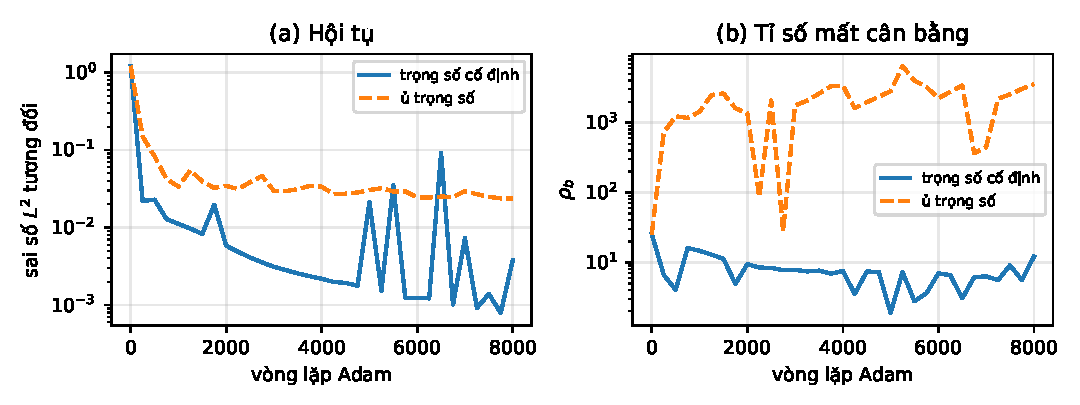
\includegraphics[width=\textwidth]{Images/chap_5/fig54_heat.pdf}
\caption{Phương trình khuếch tán. (a) Hội tụ sai số $L^2$ trong giai đoạn Adam.
(b) Chỉ số mất cân bằng $\rho_b$: với trọng số cố định, $\rho_b$ giảm dần -- theo
Định nghĩa~\ref{dn:rho}, đây là dấu hiệu không có bệnh lý gradient.}
\label{fig:tn4}
\end{figure}
 
\begin{nhanxet}[Điều kiện áp dụng của Thuật toán~\ref{alg:annealing}]
\label{nx:dieu-kien-anneal}
Kết quả trên không bác bỏ Thuật toán~\ref{alg:annealing} mà \emph{xác định phạm vi
áp dụng} của nó. Quy tắc \eqref{eq:lambda-hat} chỉ nhằm làm cân bằng biên độ
gradient; không có kết quả nào trong Chương~\ref{chap:pinn} khẳng định việc cân
bằng ấy luôn cải thiện độ chính xác, và Nhận xét~\ref{nx:danh-doi} đã cho một cơ
chế cụ thể khiến nó có thể làm xấu đi.
 
Khuyến nghị rút ra: \emph{đo $\rho_b$ trước, bật ủ trọng số sau}. Nếu $\rho_b$ nhỏ
hoặc có xu hướng giảm, giữ trọng số cố định. Chi phí của phép đo này, theo
Mục~\ref{ssec:rho}, là không đáng kể so với việc chạy hỏng cả một phiên huấn
luyện.
\end{nhanxet}
 
%==============================================================================
\section{Thí nghiệm 5: phương trình Burgers độ nhớt nhỏ}
\label{sec:tn5}
%==============================================================================
 
\begin{equation}
\left\{
\begin{aligned}
&\partial_t u + u\,\partial_x u - \nu\,\partial_{xx} u = 0,
  && (x,t) \in (-1,1)\times(0,1], \quad \nu = \tfrac{0{,}01}{\pi},\\
&u(x,0) = -\sin(\pi x), \quad u(-1,t) = u(1,t) = 0.
\end{aligned}
\right.
\label{eq:burgers-tn5}
\end{equation}
 
Đây là bài toán mà cả ba tầng của Bảng~\ref{tab:ba-nguyen-nhan} cùng bất lợi: hằng
số ổn định cỡ $1/(\pi^2\nu) \approx 31{,}8$, lớp trong đòi hỏi tần số
$\abs{k}\sim 77$, và toán tử bậc hai khuếch đại phổ theo $\norm{k}^2$.
 
\textbf{Nghiệm tham chiếu.} Bài toán \eqref{eq:burgers-tn5} không có nghiệm đóng
dạng sơ cấp, nên ta dựng nghiệm tham chiếu bằng sai phân hữu hạn bậc hai kết hợp
Runge--Kutta bậc bốn tường minh: dạng bảo toàn $\big(u^2/2\big)_x$ sai phân trung
tâm, khuếch tán sai phân trung tâm ba điểm, $N_x = 2\,047$ điểm trong,
$\Delta t = 5\times10^{-5}$. Số Péclet lưới
$\mathrm{Pe} = \max\abs{u}\,\Delta x/\nu \approx 0{,}31 < 2$ bảo đảm sai phân
trung tâm không dao động. Kiểm chứng hội tụ lưới bằng cách so với lần chạy
$N_x = 1\,023$ cho sai lệch $L^2$ tương đối $2{,}31\times10^{-4}$, nhỏ hơn hai bậc
so với sai số PINN cần đo, nên nghiệm tham chiếu đủ chính xác để làm chuẩn.
 
Nghiệm tham chiếu cho $\max_x\abs{\partial_x u} = 150{,}1$ tại $t = 0{,}5$, xác
nhận sự tồn tại của lớp trong sắc nét mà Mục~\ref{subsec:thang-do-dai} dự báo. Thời
điểm hình thành khớp với giá trị lý thuyết cho phương trình Burgers không nhớt,
$t_b = 1/\max\abs{u_0'} = 1/\pi \approx 0{,}318$.
 
\begin{nhanxet}[Cần thống nhất một nghiệm tham chiếu duy nhất]
\label{nx:hai-nghiem-tham-chieu}
Mục~\ref{subsec:thang-do-dai} trích $\max\abs{u_x} \approx 151$ tại
$t \approx 0{,}51$ từ một nghiệm giả phổ Fourier với $2\,048$ chế độ, còn mục này
trích $150{,}1$ tại $t = 0{,}5$ từ nghiệm sai phân hữu hạn. Hai con số nhất quán
với nhau trong phạm vi sai số của cả hai lược đồ, nhưng chúng đến từ \emph{hai
nghiệm tham chiếu khác nhau}. Khi hoàn thiện luận văn, cần chọn một nghiệm tham
chiếu duy nhất và dùng nó ở cả hai chương, đồng thời nêu rõ lược đồ và tham số rời
rạc hoá đúng một lần.
\end{nhanxet}
 
\textbf{Thiết lập PINN.} $N_r = 2\,500$, $N_b = 300$, $N_0 = 300$; $6\,000$ vòng
Adam rồi L-BFGS.
 
\begin{table}[H]
\centering
\caption{Phương trình Burgers \eqref{eq:burgers-tn5} so với nghiệm tham chiếu sai
phân hữu hạn.}
\label{tab:tn5}
\small
\begin{tabular}{@{}lrrrr@{}}
\toprule
\textbf{Chiến lược} & $\varepsilon_{L^2}$ (Adam) & $\varepsilon_{L^2}$ (cuối)
& $\varepsilon_{L^{\infty}}$ & $\lambda_b$ cuối \\
\midrule
Trọng số cố định
& $4{,}525\times10^{-2}$ & $\mathbf{2{,}837\times10^{-2}}$
& $4{,}348\times10^{-1}$ & $1{,}00$ \\
Ủ trọng số, $\alpha = 0{,}9$
& $6{,}230\times10^{-1}$ & $4{,}512\times10^{-1}$
& $1{,}008\times10^{0}$ & $6{,}01\times10^{4}$ \\
Ủ trọng số, $\alpha = 0{,}1$
& $5{,}959\times10^{-1}$ & $4{,}489\times10^{-1}$
& $1{,}037\times10^{0}$ & $1{,}45\times10^{5}$ \\
\bottomrule
\end{tabular}
\end{table}
 
\begin{figure}[H]
\centering
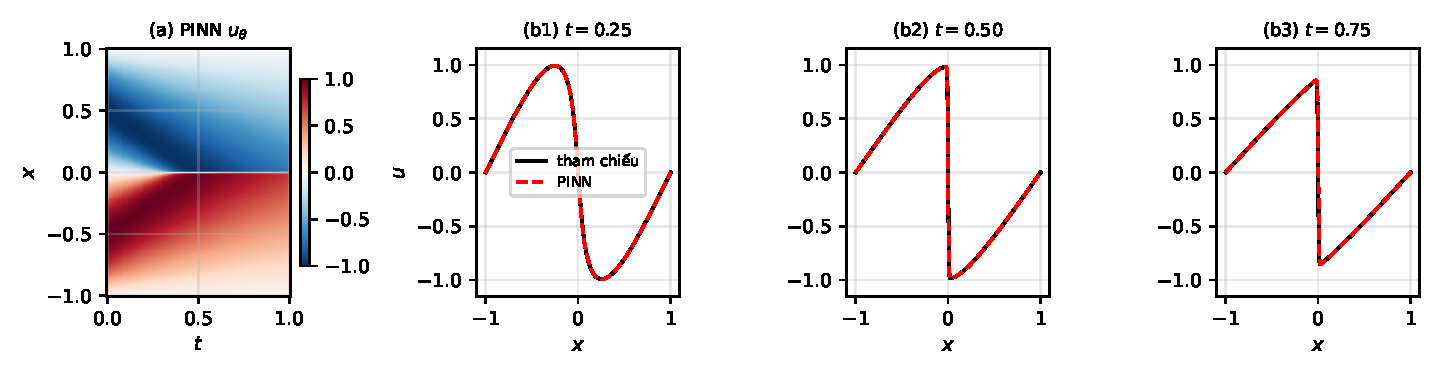
\includegraphics[width=\textwidth]{Images/chap_5/fig55_burgers.pdf}
\caption{Nghiệm PINN cho phương trình Burgers với $\nu = 0{,}01/\pi$. (a) Trường
nghiệm $u_{\btheta}(x,t)$. (b1)--(b3) Lát cắt theo thời gian so với nghiệm tham
chiếu.}
\label{fig:tn5}
\end{figure}
 
\textbf{Kết quả 1: bệnh lý gradient xuất hiện đúng như dự báo.}
Hình~\ref{fig:tn6}(a) cho phép so sánh trực tiếp hai bài toán:
\begin{equation}
\max\rho_b\big|_{\text{Burgers}} = 1\,758{,}2
\qquad\text{so với}\qquad
\max\rho_b\big|_{\text{khuếch tán}} = 25{,}4,
\label{eq:so-sanh-rho}
\end{equation}
tức chênh nhau $69{,}2$ lần. Quan trọng hơn con số tuyệt đối là \emph{xu hướng}:
với Burgers, $\rho_b$ \emph{tăng} từ $14{,}4$ tại khởi tạo lên $1\,758{,}2$ sau
$6\,000$ vòng, trong khi với khuếch tán nó giảm. Đây đúng là điều kiện thứ hai
trong Định nghĩa~\ref{dn:rho}, và nó chỉ xuất hiện ở bài toán cứng -- kết quả này
xác nhận bệnh lý gradient là hiện tượng \emph{phụ thuộc bài toán}, không phải đặc
tính cố hữu của mọi PINN.
 
\textbf{Kết quả 2: cơ chế khuếch đại -- quan sát chưa có chứng minh.} Ta đo
$\norm{\bW^{(1)}}_F$ tăng từ $1{,}83$ lên $3{,}68$, tức
$\norm{\bW^{(1)}}_F^2$ tăng $4{,}04$ lần, trong khi $\rho_b$ tăng $122$ lần. Hai
đại lượng cùng tăng đơn điệu và cùng lúc (Hình~\ref{fig:tn6}b), gợi ý một mối liên
hệ giữa chuẩn trọng số lớp vào và mức mất cân bằng gradient.
 
Cần nói rõ giới hạn của quan sát này. Luận văn \emph{không} có mệnh đề nào chứng
minh $\rho_b \sim \norm{\bW^{(1)}}^2$; đây là một tương quan quan sát được trên
một lần chạy, không phải một dự báo được kiểm chứng. Hệ số $4{,}04$ cũng không
giải thích được hệ số $122$, nên nếu có một quan hệ luỹ thừa thì số mũ phải lớn
hơn $1$ đáng kể. Một hướng giải thích khả dĩ, phù hợp với
Mệnh đề~\ref{md:jacobian}: $\partial_{xx}u_{\btheta}$ theo truy hồi
\eqref{eq:S-truy-hoi} chứa tích của các $\bW^{(\ell)}$ ở \emph{mọi} lớp, không chỉ
lớp đầu, nên chuẩn của một lớp không đủ để giải thích. Ta ghi nhận đây là câu hỏi
để ngỏ chứ không kết luận.
 
\begin{figure}[H]
\centering
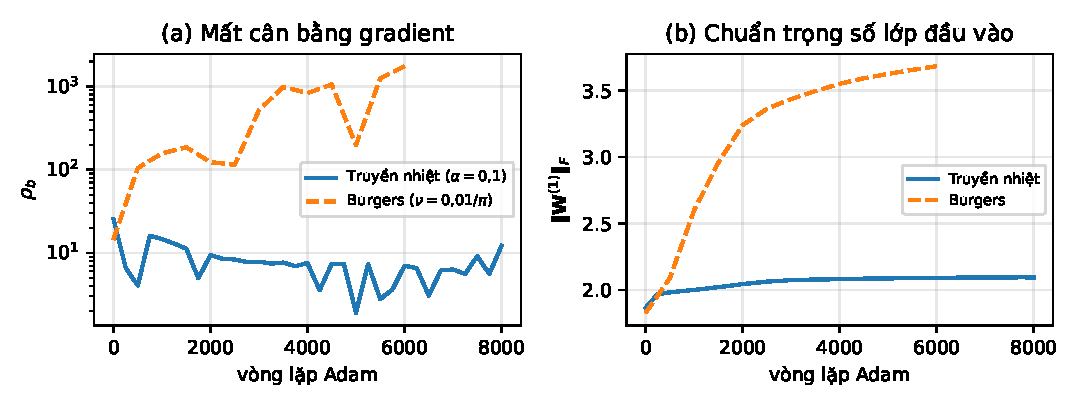
\includegraphics[width=\textwidth]{Images/chap_5/fig56_rho.pdf}
\caption{So sánh hai bài toán. (a) $\rho_b$ tăng đơn điệu với Burgers, giảm với
khuếch tán. (b) Chuẩn Frobenius của ma trận trọng số lớp vào.}
\label{fig:tn6}
\end{figure}
 
\textbf{Kết quả 3: ủ trọng số thất bại cả trên bài toán cứng.} Đây là kết quả cần
thận trọng nhất trong chương. Ủ trọng số làm sai số xấu đi $15{,}9$ lần
($2{,}84\times10^{-2} \to 4{,}51\times10^{-1}$), với $\lambda_b$ chạy tới
$6{,}01\times10^4$. Vì bài toán này \emph{thực sự} có bệnh lý gradient theo
\eqref{eq:so-sanh-rho}, không thể giải thích bằng
Nhận xét~\ref{nx:dieu-kien-anneal}.
 
Trước khi kết luận, ta loại trừ hai giả thuyết cạnh tranh.
 
\emph{(i) Sai công thức?} Công thức cài đặt trùng với \eqref{eq:lambda-hat} của
Chương~\ref{chap:pinn}, vốn được đối chiếu trực tiếp với Thuật toán 2.1
của~\cite{wang2021}.
 
\emph{(ii) Sai hệ số làm trơn?} Với quy tắc \eqref{eq:lambda-update}, giá trị
$\alpha$ nhỏ làm trơn mạnh còn $\alpha$ gần $1$ nghiêng hẳn về ước lượng mới; bài
báo gốc khuyến nghị $\alpha = 0{,}1$. (Ký hiệu $\alpha$ ở đây là hệ số làm trơn
của \eqref{eq:lambda-update}, không liên quan tới hệ số khuếch tán $\nu$ của
\eqref{eq:heat}.) Ta chạy lại với cả hai giá trị. Hai dòng cuối
Bảng~\ref{tab:tn5} cho kết quả gần như nhau ($4{,}51\times10^{-1}$ so với
$4{,}49\times10^{-1}$), nên kết luận không nhạy với lựa chọn này.
 
Nguyên nhân thực sự là một \emph{bất ổn định phản hồi dương} nằm ngay trong cấu
trúc của quy tắc \eqref{eq:lambda-hat}, và có thể chứng minh được.
 
\begin{bode}[Phản hồi dương của quy tắc cân bằng trọng số]
\label{bd:phan-hoi-duong}
Giả sử thành phần thứ $i$ có dạng
$J_i(\btheta) = \frac{1}{N_i}\sum_{j=1}^{N_i} g_j(\btheta)^2$ với
$g_j \in C^1$ và $\norm{\nabla g_j(\btheta)} \le G_i$ trên miền đang xét. Khi đó
\begin{equation}
\norm{\nabla_{\btheta} J_i(\btheta)}_{1}
 \;\le\; 2\,G_i\,\sqrt{P}\;\sqrt{J_i(\btheta)} ,
\label{eq:grad-le-sqrt}
\end{equation}
và do đó, với $\hat\lambda_i$ cho bởi \eqref{eq:lambda-hat},
\begin{equation}
\hat{\lambda}_i(\btheta)
 \;\ge\; \frac{\sqrt{P}\;\norm{\nabla_{\btheta}J_r(\btheta)}_{\infty}}
              {2G_i}\cdot\frac{1}{\sqrt{J_i(\btheta)}}
 \;\xrightarrow[\;J_i \to 0\;]{}\; +\infty ,
\label{eq:lambda-phan-ky}
\end{equation}
miễn là $\norm{\nabla_{\btheta}J_r}_{\infty}$ bị chặn dưới bởi một hằng số dương.
\end{bode}
 
\begin{proof}
Ta có $\nabla J_i = \frac{2}{N_i}\sum_j g_j \nabla g_j$, nên theo bất đẳng thức
tam giác rồi Cauchy--Schwarz trên chỉ số $j$,
\begin{align*}
\norm{\nabla J_i}_{2}
 &\le \frac{2}{N_i}\sum_j \abs{g_j}\,\norm{\nabla g_j}_2
  \le \frac{2G_i}{N_i}\sum_j \abs{g_j}
  \le \frac{2G_i}{N_i}\sqrt{N_i}\Big(\sum_j g_j^2\Big)^{1/2}\\
 &= \frac{2G_i}{N_i}\sqrt{N_i}\cdot\sqrt{N_i J_i}
  = 2G_i\sqrt{J_i},
\end{align*}
trong đó bước cuối dùng $\sum_j g_j^2 = N_i J_i$ theo định nghĩa của $J_i$.
Chuyển sang chuẩn $L^1$ trên $\R^P$ bằng
$\norm{\bm{v}}_1 \le \sqrt{P}\,\norm{\bm{v}}_2$ cho
\eqref{eq:grad-le-sqrt}. Thay vào mẫu số của \eqref{eq:lambda-hat}, vốn bằng
$\tfrac{1}{P}\norm{\nabla J_i}_1$, được \eqref{eq:lambda-phan-ky}.
\end{proof}
 
Bổ đề~\ref{bd:phan-hoi-duong} cho chính xác cơ chế hỏng. Khi $J_i$ giảm, mẫu số
của \eqref{eq:lambda-hat} giảm ít nhất theo $\sqrt{J_i}$, làm $\hat{\lambda}_i$
tăng, khiến thành phần $i$ được ưu tiên hơn nữa và $J_i$ giảm nhanh hơn nữa. Vòng
phản hồi này \emph{không có cơ chế tự hãm}: cận dưới \eqref{eq:lambda-phan-ky}
phân kỳ như $J_i^{-1/2}$.
 
Số liệu khớp với dự báo. Trong lần chạy có ủ, $\rho_b$ đạt $1{,}69\times10^5$, tức
cao gấp $96$ lần lần chạy không ủ -- thuật toán nhằm \emph{giảm} mất cân bằng lại
làm nó trầm trọng hơn hai bậc độ lớn. Và theo
Nhận xét~\ref{nx:danh-doi}, $\lambda_b$ ở thang $10^4$--$10^5$ nằm xa quá mức giá
trị hữu hạn tối ưu, nên phần dư trong miền bị hy sinh hoàn toàn.
 
\begin{nhanxet}[Kết luận thực hành về ủ trọng số]
\label{nx:ket-luan-anneal}
Trên cả hai bài toán khảo sát, Thuật toán~\ref{alg:annealing} ở dạng nguyên bản
đều làm giảm độ chính xác, và Bổ đề~\ref{bd:phan-hoi-duong} cho thấy đây không
phải trùng hợp mà là hệ quả cấu trúc của quy tắc \eqref{eq:lambda-hat} khi
$J_i \to 0$. Hai hướng khắc phục theo đúng cơ chế vừa chứng minh: đặt chặn trên
cho $\lambda_i$, hoặc thay mẫu số bằng một đại lượng không triệt tiêu cùng $J_i$
-- chẳng hạn vết của nhân tiếp tuyến thay cho chuẩn gradient.
 
Với phạm vi luận văn này, khuyến nghị là dùng trọng số cố định kèm dò tìm
$\lambda_b$ theo Bảng~\ref{tab:tn2}, và xem việc ủ trọng số như một hướng cần khảo
sát thêm. Cần nêu rõ rằng kết luận này \emph{không} bác bỏ kết quả
của~\cite{wang2021}, vốn báo cáo cải thiện hơn một bậc độ lớn trên bài toán
Helmholtz: sự khác biệt có thể nằm ở bài toán, ở ngân sách huấn luyện, hoặc ở chi
tiết cài đặt mà ta chưa tái lập được. Điều Bổ đề~\ref{bd:phan-hoi-duong} khẳng
định là quy tắc có một chế độ hỏng xác định, không phải là nó luôn hỏng.
\end{nhanxet}
 
\textbf{Kết quả 4: chất lượng nghiệm.} Với trọng số cố định, PINN đạt
$\varepsilon_{L^2} = 2{,}84\times10^{-2}$.
Hình~\ref{fig:tn5}(b2)--(b3) cho thấy lớp trong tại $x = 0$ được tái tạo. Chênh
lệch lớn giữa $\varepsilon_{L^2} = 2{,}84\times10^{-2}$ và
$\varepsilon_{L^{\infty}} = 4{,}35\times10^{-1}$ -- hệ số $15$ lần -- có ý nghĩa
cấu trúc: sai số hầu như tập trung toàn bộ vào một dải hẹp quanh $x = 0$, đúng như
phân tích ba tầng ở Bảng~\ref{tab:ba-nguyen-nhan} dự báo. Bậc sai số trung bình
vẫn chấp nhận được, nhưng đúng chỗ quan trọng nhất về mặt vật lý thì sai số lớn
nhất.
 
%==============================================================================
\section{Thí nghiệm 6: kiểm chứng chặn ổn định}
\label{sec:tn6}
%==============================================================================

\begin{thinghiem}[Kiểm chứng Mệnh đề~\ref{md:chan-on-dinh}]
\label{tn:chan}
Mệnh đề~\ref{md:chan-on-dinh} là mắt xích biện minh cho toàn bộ phương pháp: nó
nói rằng cực tiểu hoá một đại lượng \emph{tính được} ($\norm{r_{\btheta}}$) khống
chế được đại lượng \emph{quan tâm} ($\norm{e_{\btheta}}$). Nhưng chặn ấy có một
giả thiết dễ bị bỏ qua: điều kiện biên phải được thoả \emph{chính xác}. Câu hỏi:
chặn có đúng trong thực tế không, nó chặt đến đâu, và điều gì xảy ra khi giả
thiết bị vi phạm?
\end{thinghiem}

\textbf{Thiết lập.} Vẫn bài toán Poisson \eqref{eq:poisson-tn1}. Ta đo đồng thời
$\norm{r_{\btheta}}_{L^2}$, $\norm{e_{\btheta}}_{L^2}$ và
$\norm{e_{\btheta}'}_{L^2}$ trên lưới đánh giá $20\,001$ điểm bằng quy tắc hình
thang, tại sáu mốc trải suốt quá trình huấn luyện để quét được bốn bậc độ lớn
của phần dư. Ba cấu hình tách bạch vai trò của giả thiết:

\begin{enumerate}[label=(\alph*),leftmargin=2.2em,itemsep=2pt]
\item \textbf{Ràng buộc cứng} $\hat u_{\btheta}(x) = x(1-x)\,u_{\btheta}(x)$ theo
Bổ đề~\ref{bd:rang-buoc-cung}, với $D(x) = x(1-x)$ đúng như dạng được đề nghị ở
Mục~\ref{subsec:rang-buoc}. Điều kiện biên thoả chính xác với mọi $\btheta$, tức
giả thiết của mệnh đề được \emph{thoả theo cấu trúc}.
\item \textbf{Ràng buộc mềm, $\lambda_b = 100$} -- giá trị tốt nhất theo
Bảng~\ref{tab:tn2}. Giả thiết chỉ thoả gần đúng.
\item \textbf{Ràng buộc mềm, $\lambda_b = 0{,}01$} -- giá trị mà
Bảng~\ref{tab:tn2} cho thấy sai số biên bão hoà ở mức $0{,}91$. Giả thiết bị vi
phạm nặng.
\end{enumerate}

\begin{table}[H]
\centering
\caption[Kiểm chứng chặn ổn định của Mệnh đề~\ref{md:chan-on-dinh}]{Kiểm chứng
chặn $\norm{e_{\btheta}}_{L^2} \le \pi^{-2}\norm{r_{\btheta}}_{L^2}$. Cột
``tỉ số'' là $\norm{e_{\btheta}}_{L^2}/\norm{r_{\btheta}}_{L^2}$; chặn được thoả
khi tỉ số này không vượt $\pi^{-2} \approx 0{,}1013$.}
\label{tab:tn6}
\small
\setlength{\tabcolsep}{4pt}
\begin{tabular}{@{}l rrr r c@{}}
\toprule
\textbf{Mốc} & $\norm{r_{\btheta}}_{L^2}$ & $\norm{e_{\btheta}}_{L^2}$
& sai số biên & tỉ số & thoả chặn? \\
\midrule
\multicolumn{6}{@{}l}{\emph{(a) Ràng buộc cứng --- giả thiết thoả chính xác}}\\
Khởi tạo   & $2{,}809\times10^{1}$ & $7{,}115\times10^{-1}$ & $0$ & $0{,}0253$ & có \\
Adam $200$ & $5{,}735\times10^{0}$ & $3{,}705\times10^{-2}$ & $0$ & $0{,}0065$ & có \\
Adam $1000$& $1{,}511\times10^{-1}$& $4{,}173\times10^{-4}$ & $0$ & $0{,}0028$ & có \\
Adam $4000$& $2{,}526\times10^{-2}$& $6{,}109\times10^{-5}$ & $0$ & $0{,}0024$ & có \\
$+$ L-BFGS & $2{,}599\times10^{-3}$& $1{,}815\times10^{-6}$ & $0$ & $0{,}0007$ & có \\
\addlinespace
\multicolumn{6}{@{}l}{\emph{(b) Ràng buộc mềm, $\lambda_b = 100$}}\\
Adam $1000$& $1{,}663\times10^{-1}$& $7{,}820\times10^{-3}$ & $1{,}7\times10^{-2}$ & $0{,}0470$ & có \\
$+$ L-BFGS & $4{,}214\times10^{-3}$& $5{,}029\times10^{-6}$ & $9{,}9\times10^{-6}$ & $0{,}0012$ & có \\
\addlinespace
\multicolumn{6}{@{}l}{\emph{(c) Ràng buộc mềm, $\lambda_b = 0{,}01$}}\\
Adam $200$ & $4{,}033\times10^{0}$ & $2{,}923\times10^{0}$  & $5{,}21$ & $0{,}7248$ & \textbf{không} \\
Adam $1000$& $9{,}087\times10^{-2}$& $8{,}736\times10^{-1}$ & $1{,}52$ & $\mathbf{9{,}614}$ & \textbf{không} \\
Adam $4000$& $2{,}976\times10^{-2}$& $2{,}906\times10^{-1}$ & $0{,}503$& $\mathbf{9{,}763}$ & \textbf{không} \\
$+$ L-BFGS & $4{,}304\times10^{-3}$& $1{,}127\times10^{-3}$ & $2{,}1\times10^{-3}$ & $0{,}2618$ & \textbf{không} \\
\bottomrule
\end{tabular}
\end{table}

\textbf{Kết quả.} Ba kết luận, mỗi kết luận trả lời một phần của câu hỏi đặt ra.

\emph{(a) Chặn đúng, và đúng trên toàn dải.} Với ràng buộc cứng, tỉ số
$\norm{e_{\btheta}}/\norm{r_{\btheta}}$ nằm dưới $\pi^{-2}$ tại \emph{mọi} mốc,
trong khi $\norm{r_{\btheta}}$ quét bốn bậc độ lớn từ $2{,}81\times10^{1}$ xuống
$2{,}60\times10^{-3}$. Chặn cho đạo hàm cũng đúng: tỉ số
$\norm{e_{\btheta}'}/\norm{r_{\btheta}}$ cao nhất là $0{,}159$, dưới
$\pi^{-1}\approx 0{,}318$.

\emph{(b) Chặn không chặt.} Tỉ số quan sát được nằm trong khoảng
$0{,}0007$--$0{,}0261$, tức nhỏ hơn hằng số $\pi^{-2}$ từ $4$ đến $145$ lần. Điều
này không mâu thuẫn với mệnh đề: hằng số $\pi^{-2}$ là tối ưu trên \emph{toàn bộ}
lớp hàm $H^1_0(0,1)$, đạt được khi sai số trùng hàm riêng $\sin \pi x$ ứng với
trị riêng nhỏ nhất. Sai số của mạng nơ-ron ở đây không có dạng ấy, nên chặn còn
dư địa. Hệ quả thực hành: chặn dùng được như một \emph{bảo đảm}, không dùng được
như một \emph{ước lượng} sai số.

\emph{(c) Giả thiết điều kiện biên là thiết yếu, không phải trang trí.} Với
$\lambda_b = 0{,}01$, chặn bị vi phạm ở mọi mốc sau khởi tạo, và mức vi phạm lên
tới $9{,}76$ so với $0{,}1013$ --- tức \emph{gấp $96$ lần}. Đọc dòng
``Adam $4000$'' cho thấy rõ cơ chế: phần dư đã nhỏ
($\norm{r_{\btheta}} = 2{,}98\times10^{-2}$) trong khi sai số vẫn lớn
($\norm{e_{\btheta}} = 2{,}91\times10^{-1}$, gấp mười lần phần dư). Đây chính là
kịch bản mà Nhận xét~\ref{rem:ill-posedness} mô tả: mạng trôi trên tập
$\mathcal{M}_r$ của \eqref{eq:manifold-r} và hội tụ về \emph{một nghiệm khác} của
cùng phương trình vi phân.

\begin{nhanxet}[Vì sao thí nghiệm này đáng làm]
\label{nx:y-nghia-tn6}
Đây là thí nghiệm duy nhất trong chương kiểm chứng trực tiếp mắt xích
\emph{logic} của phương pháp chứ không phải một hiện tượng của mô hình. Nó cho
một quy tắc thực hành cụ thể: chỉ khi điều kiện biên được thoả (chính xác bằng
ràng buộc cứng, hoặc tới độ chính xác cao bằng $\lambda_b$ đủ lớn) thì việc theo
dõi $J_r$ mới là chỉ báo hợp lệ cho sai số. Ở chế độ $\lambda_b$ nhỏ, một giá trị
$J_r$ nhỏ \emph{không} nói gì về chất lượng nghiệm --- và đó là chế độ mà bệnh lý
gradient (Mục~\ref{sec:gradient-pathology}) tự động đẩy bài toán vào khi
$\lambda_b$ không được chọn cẩn thận.
\end{nhanxet}

%==============================================================================
\section{Đối chiếu lý thuyết và thực nghiệm}
\label{sec:doi-chieu}
%==============================================================================
 
\begin{table}[H]
\centering
\caption{Đối chiếu giữa các kết quả lý thuyết và số liệu đo được.}
\label{tab:doi-chieu}
\small
\begin{tabular}{@{}p{2.9cm}p{3.7cm}p{3.9cm}p{3.0cm}@{}}
\toprule
\textbf{Kết quả} & \textbf{Dự báo} & \textbf{Đo được} & \textbf{Kết luận} \\
\midrule
Hệ quả~\ref{hq:pinn-hong}
& $\nabla_{\btheta}J_r \equiv \bm{0}$ với ReLU
& $\norm{\nabla J_r}_\infty = 0{,}0$; $J_r = 776{,}23$ so với $778{,}49$ trên
  lưới đánh giá
& \textbf{Khớp chính xác} \\[4pt]
Mệnh đề~\ref{md:phat-bien-phat}
& sai số biên $\propto \lambda_b^{-1}$
& số mũ đo được $-0{,}907$; bão hoà ở hai đầu
& \textbf{Khớp}, lệch $9\%$ ở số mũ \\[4pt]
Mục~\ref{subsec:adam-vs-lbfgs}
& tựa Newton vượt điều kiện số xấu và sàn nhiễu
& cải thiện $28{,}6$ lần sau $500$ vòng
& \textbf{Khớp} \\[4pt]
Định nghĩa~\ref{dn:rho}
& bệnh lý chỉ ở bài toán cứng
& $\rho_b$: $1\,758$ (Burgers) so với $25{,}4$ (khuếch tán); xu hướng ngược nhau
& \textbf{Khớp} \\[4pt]
Giả thuyết \eqref{eq:pho-hieu-dung}
& phần dư ưu tiên $k$ cao
& $\abs{c_1}/\abs{c_8} = 38{,}6$; thứ tự học đảo chiều so với hồi quy
& \textbf{Khớp về hướng} \\[4pt]
Mục~\ref{subsec:he-qua-pinn}
& lớp sốc học chậm nhất
& với Poisson thì ngược lại
& \textbf{Cần siết lại} (Nhận xét~\ref{nx:hieu-chinh}) \\[4pt]
Quan hệ $\rho_b$--$\norm{\bW^{(1)}}^2$
& (không có mệnh đề)
& $\norm{\bW^{(1)}}^2$ tăng $4{,}04$ lần, $\rho_b$ tăng $122$ lần
& \textbf{Tương quan}, chưa giải thích \\[4pt]
Thuật toán~\ref{alg:annealing}
& cân bằng biên độ gradient
& làm xấu $35{,}6$ lần (khuếch tán), $15{,}9$ lần (Burgers)
& \textbf{Có chế độ hỏng} (Bổ đề~\ref{bd:phan-hoi-duong}) \\[4pt]
Mệnh đề~\ref{md:chan-on-dinh}
& $\norm{e}_{L^2}\le \pi^{-2}\norm{r}_{L^2}$ khi điều kiện biên thoả chính xác
& tỉ số $\le 0{,}026$ trên bốn bậc độ lớn của $\norm{r}$; vi phạm $96$ lần khi
  $\lambda_b = 0{,}01$
& \textbf{Khớp}, và giả thiết biên tỏ ra thiết yếu \\
\bottomrule
\end{tabular}
\end{table}
 
Trong chín hạng mục: năm khớp trọn vẹn, một khớp về hướng nhưng không rút được
kết luận định lượng, một cần siết lại cách phát biểu, một chỉ là tương quan chưa
giải thích được, và một cho kết quả tiêu cực nhưng đã truy được nguyên nhân.
 
Mức khớp này ủng hộ khung lý thuyết của Chương~\ref{chap:pinn} một cách
\emph{có điều kiện}, và điều kiện ấy đáng được nêu rõ: bốn trong năm hạng mục
khớp trọn vẹn tương ứng với một mệnh đề \emph{đã được chứng minh}
(Hệ quả~\ref{hq:pinn-hong}, Mệnh đề~\ref{md:phat-bien-phat},
Mệnh đề~\ref{md:san-nhieu}, Mệnh đề~\ref{md:chan-on-dinh}); hạng mục còn lại dựa trên
Định nghĩa~\ref{dn:rho}, vốn là một \emph{tiêu chí chẩn đoán} do luận văn đặt ra
chứ không phải một mệnh đề, nên nó kiểm chứng tính hữu dụng của tiêu chí chứ
không kiểm chứng một dự báo lý thuyết. Ngược lại, cả ba hạng mục có vấn đề đều
tương ứng với những chỗ luận văn dùng \emph{suy luận tiệm cận} hoặc \emph{ghép
hai kết quả rời rạc}:
giả thuyết \eqref{eq:pho-hieu-dung} ghép $\abs{P}^2$ với
$\widehat{\varkappa}$; kết luận ở Mục~\ref{subsec:he-qua-pinn} ngầm giả định thừa
số nào thắng; quan hệ $\rho_b$--$\norm{\bW^{(1)}}^2$ không có chứng minh nào cả.
 
Đây là bài học phương pháp luận của chương, và nó nhất quán với ranh giới mà
Chương~\ref{chap:fnn} đã vạch giữa lý thuyết xấp xỉ và lý thuyết tối ưu: những gì
được chứng minh thì đứng vững, những gì được suy đoán thì cần kiểm chứng trước khi
dùng.
 
%==============================================================================
\section{Hạn chế của thiết kế thực nghiệm}
\label{sec:hanche}
%==============================================================================
 
Để các kết luận trên được đọc đúng phạm vi, cần nêu rõ những hạn chế sau.
 
\begin{enumerate}[label=(\arabic*),leftmargin=2.2em,itemsep=4pt]
\item \emph{Một hạt giống ngẫu nhiên duy nhất.} Mọi lần chạy dùng một hạt giống cố
định để tái lập được, nên không có ước lượng độ phân tán giữa các lần khởi tạo.
Đây là vi phạm trực tiếp nguyên tắc đã nêu ở Nhận xét~\ref{nx:doi-xung-hoan-vi}:
với ít nhất $2^{n_1}n_1!$ cực tiểu tương đương, một kết quả tốt từ một hạt giống
may mắn không phải bằng chứng về phương pháp. Hệ quả thực hành cho việc đọc chương
này: các chênh lệch dưới hai lần trong bảng số liệu \emph{không nên} được coi là
có ý nghĩa; mọi kết luận ở Mục~\ref{sec:doi-chieu} đều dựa trên chênh lệch từ một
bậc độ lớn trở lên. Khắc phục đúng cách là lặp mỗi cấu hình trên $5$--$10$ hạt
giống và báo cáo trung vị cùng khoảng phân vị.
 
\item \emph{Ngân sách huấn luyện hạn chế.} Toàn bộ thí nghiệm chạy trên một lõi
CPU, với $4\,000$--$8\,000$ vòng Adam, so với bậc $10^5$ vòng thường dùng trong
các công trình gốc~\cite{raissi2019}. Sai số Burgers $2{,}84\times10^{-2}$ vì vậy
\emph{không} phản ánh giới hạn của phương pháp PINN mà phản ánh giới hạn của ngân
sách; các công trình gốc báo cáo bậc $10^{-3}$--$10^{-4}$ trên cùng bài toán với
mạng lớn hơn và huấn luyện lâu hơn.
 
\item \emph{Mạng nhỏ.} Kiến trúc $2\,209$--$8\,513$ tham số nhỏ hơn đáng kể so với
chuẩn mực trong tài liệu. Nói riêng, lập luận NTK ở Nhận xét~\ref{rem:ntk-view}
giả thiết chế độ nhân tiếp tuyến \emph{hằng} (mạng vô hạn rộng); với mạng cỡ này
giả thiết ấy chỉ đúng gần đúng, nên Thí nghiệm~\ref{tn:pho} phải được hiểu là kiểm
chứng \emph{định tính} về thứ tự học, không phải kiểm chứng định lượng phổ NTK.
Đây cũng là lý do ta không rút kết luận số từ đối chiếu $38{,}6$ với $64$ ở
Mục~\ref{sec:tn3}.
 
\item \emph{Chưa khảo sát độ nhạy theo cách lấy mẫu.} Cả lấy mẫu siêu khối Latin
lẫn lấy mẫu thích nghi RAR ở Bảng~\ref{tab:remedies} đều chưa được kiểm chứng.
Riêng với bài toán Burgers ở Mục~\ref{sec:tn5}, nơi sai số tập trung vào một
dải hẹp quanh
$x = 0$, RAR là kỹ thuật có khả năng cải thiện rõ nhất và đáng được thử trước
tiên.
 
\item \emph{Nghiệm tham chiếu cho Burgers là nghiệm số.} Dù đã kiểm chứng hội tụ
lưới ($2{,}31\times10^{-4}$), đây vẫn không phải nghiệm giải tích, nên kết luận về
Burgers có thêm một tầng sai số so với bài toán khuếch tán ở
Mục~\ref{sec:tn4}. Thêm vào đó,
Nhận xét~\ref{nx:hai-nghiem-tham-chieu} đã nêu việc hai chương hiện dùng hai nghiệm
tham chiếu khác nhau.
 
\item \emph{Chặn ổn định mới được kiểm chứng ở trường hợp đơn giản nhất.}
Mục~\ref{sec:tn6} đã kiểm chứng Mệnh đề~\ref{md:chan-on-dinh} trên bài toán
Poisson. Nhưng Mệnh đề~\ref{md:chan-suy-bien} --- vốn mới là tầng thứ nhất của
Bảng~\ref{tab:ba-nguyen-nhan} --- thì chưa: sự suy biến của hằng số ổn định theo
$1/\nu$ đòi hỏi quét $\nu$ trên bài toán đối lưu--khuếch tán, và phép quét ấy
chưa được thực hiện. Đây là bổ sung có giá trị nhất còn lại cho chương này.
\end{enumerate}
 
%==============================================================================
\section*{Kết luận chương}
\addcontentsline{toc}{section}{Kết luận chương}
%==============================================================================
 
Chương này đã hiện thực hoá khung lý thuyết của Chương~\ref{chap:pinn} trên
PyTorch và đưa ra số liệu kiểm chứng cho từng phát biểu chính.
 
Về mặt \emph{kỹ thuật}, cơ chế đồ thị động cùng cờ \texttt{create\_graph=True} đủ
để hiện thực trực tiếp các truy hồi \eqref{eq:G-truy-hoi} và
\eqref{eq:S-truy-hoi} mà không cần lập trình tường minh $\sigma''$, đúng như
Mệnh đề~\ref{md:ad-tai-tao} bảo đảm; độ chính xác kép là điều kiện cần để phân
biệt sai số xấp xỉ với sai số làm tròn.
 
Về mặt \emph{kiểm chứng}, ba kết quả nổi bật. Thứ nhất,
Hệ quả~\ref{hq:pinn-hong} được xác nhận tới từng chữ số máy: mạng ReLU cho
gradient bằng đúng không, chứng tỏ điều kiện $\sigma \in C^m$ là bắt buộc chứ
không phải khuyến nghị. Thứ hai, bệnh lý gradient được chứng minh là hiện tượng
\emph{phụ thuộc bài toán}: $\rho_b$ chênh nhau $69$ lần giữa Burgers và khuếch
tán, và quan trọng hơn là ngược chiều xu hướng -- nên việc chẩn đoán trước khi can
thiệp là bắt buộc. Thứ ba, giả thuyết \eqref{eq:pho-hieu-dung} được xác nhận theo
cách bất ngờ nhất: toán tử vi phân \emph{đảo ngược} thiên kiến phổ, khiến sai số
dồn về mode tần số thấp; phát hiện này buộc phải siết lại cách phát biểu ở
Mục~\ref{subsec:he-qua-pinn}.
 
Về mặt \emph{phương pháp}, hai kết quả tiêu cực có giá trị riêng. Việc tăng
$\lambda_b$ vô hạn không phải chiến lược tốt, vì sai số $L^2$ toàn cục đạt cực
tiểu tại một giá trị hữu hạn -- điều mà Mệnh đề~\ref{md:phat-bien-phat}, vốn chỉ
theo dõi sai số biên, không thể tiên đoán. Và thuật toán ủ trọng số ở dạng nguyên
bản làm giảm độ chính xác trên cả hai bài toán; ở đây thực nghiệm không chỉ phát
hiện vấn đề mà còn dẫn tới một kết quả lý thuyết mới:
Bổ đề~\ref{bd:phan-hoi-duong} chứng minh rằng quy tắc \eqref{eq:lambda-hat} có một
chế độ phản hồi dương với tốc độ phân kỳ $\hat\lambda_i \sim J_i^{-1/2}$ và không
có cơ chế tự hãm.
 
Kết quả cuối cùng ấy minh hoạ đúng vai trò của chương: bước kiểm chứng số không
chỉ xác nhận hay bác bỏ lý thuyết đã có, mà còn chỉ ra chỗ lý thuyết cần được bổ
sung.
 


%==============================================================
% TÀI LIỆU THAM KHẢO
%==============================================================

\printbibliography[
    heading=bibintoc,
    title={Tài liệu tham khảo}
]

%==============================================================
% PHỤ LỤC
%==============================================================
% Chưa bật vì hiện tại chưa có file phụ lục trong File Tree.

\end{document}